%%%%%%%%%%%%%%%%%%%% book.tex %%%%%%%%%%%%%%%%%%%%%%%%%%%%%
%
% sample root file for	 the chapters of your "monograph"
%
% Use this file as a template for your own input.
%
%%%%%%%%%%%%%%%% Springer-Verlag %%%%%%%%%%%%%%%%%%%%%%%%%%


% RECOMMENDED %%%%%%%%%%%%%%%%%%%%%%%%%%%%%%%%%%%%%%%%%%%%%%%%%%%
\documentclass[graybox,envcountchap,sectrefs]{svmono}

% choose options for [] as required from the list
% in the Reference Guide

\usepackage{mathptmx}
\usepackage{helvet}
\usepackage{courier}
\usepackage{amsmath}
\usepackage{txfonts}            % Allows bold greek letters; compatible with Springer styles.
\usepackage{type1cm}         
\usepackage{framed}
\usepackage{lscape}
\usepackage{booktabs}
\usepackage{multirow}
\usepackage{booktabs}
\usepackage[sectionbib,compress]{natbib}% provides a bibliography for each chapter
\usepackage{chapterbib}
\usepackage{makeidx}           % allows index generation
\usepackage[noprefix]{nomencl} % allows nomenclature generation
\usepackage{graphicx}          % standard LaTeX graphics tool
                               % when including figure files
\usepackage{tablefootnote}
\usepackage{scrextend}         % provides the \footref script
\usepackage{multicol}          % used for the two-column index
\usepackage[bottom]{footmisc}  % places footnotes at page bottom
\usepackage{mathtools}
\usepackage{outlines}
\usepackage{enumitem}
\usepackage[normalem]{ulem}
\usepackage{hyperref}          % Needs to come last in the list of loaded packages.

\setenumerate[1]{label=\Roman*.}
\setenumerate[2]{label=\Alph*.}
\setenumerate[3]{label=\roman*.}
\setenumerate[4]{label=\alph*.}

% Provides round-trip syncing from pdf viewer to text editor
% \usepackage{pdfsync} % Unnecessary, because pdflatex supports synctex automatically.
\synctex=1

% see the list of further useful packages
% in the Reference Guide

\makeindex{}           % used for the subject index
                       % please use the style svind.ist with
                       % your makeindex program
\makenomenclature{}    % generates the nomenclature table
\renewcommand{\nomname}{List of Symbols} % Changes the name of the nomenclature section.


%%%%%%%%%%%%%%%%%%%%%%%%%%%%%%%%%%%%%%%%%%%%%%%%%%%%%%%%%%%%%%%%%%%%%

\begin{document}

\author{Matthew Kuperus Heun, Michael Carbajales-Dale, Becky Roselius Haney}
\title{The metabolic economy}
\subtitle{A dynamic framework for material, energy, and value accounting}
\maketitle{}

\frontmatter%%%%%%%%%%%%%%%%%%%%%%%%%%%%%%%%%%%%%%%%%%%%%%%%%%%%%%

%\include{dedic}
%\include{foreword}
%\include{preface}
%\include{acknow}

\tableofcontents{}
\listoffigures{}
\listoftables{}
\printnomenclature{}   % Put the nomenclature section here.

%\include{acronym}


\mainmatter%%%%%%%%%%%%%%%%%%%%%%%%%%%%%%%%%%%%%%%%%%%%%%%%%%%%%%%

%!TEX root = ../../Heun_Dale_Haney_A_dynamic_approach_to_input_output_modeling.tex
%%%%%%%%%%%%%%%%%%%%% chapter.tex %%%%%%%%%%%%%%%%%%%%%%%%%%%%%%%%%
%
% sample chapter
%
% Use this file as a template for your own input.
%
%%%%%%%%%%%%%%%%%%%%%%%% Springer-Verlag %%%%%%%%%%%%%%%%%%%%%%%%%%
%\motto{Use the template \emph{chapter.tex} to style the various elements of your chapter content.}
\motto{Where there is no reliable accounting 
and therefore no competent knowledge
of the economic and ecological effects of our lives,
we cannot live lives that are economically
and ecologically responsible. 
It is futile to plead and protest and lobby 
in favor of public ecological responsibility while, 
in virtually every act of our private lives, 
we endorse and support an economic system 
that is by intention, 
and perhaps by necessity, 
ecologically irresponsible.~\emph{\cite[p.~26]{Berry1998}}

\hfill---\emph{Wendell Berry}}


%%%%%%%%%%%%%%%%%%%%%%%%%%%%%%%%%%
%%%%%%%%%% Introduction %%%%%%%%%%
%%%%%%%%%%%%%%%%%%%%%%%%%%%%%%%%%%
\chapter{Introduction}
% Always give a unique label
\label{chap:intro}
% use \chaptermark{}
% to alter or adjust the chapter heading in the running head
\chaptermark{Introduction}
%%%%%%%%%%%%%%%%%%%%%%%%%%%%%%%%%%
%%%%%%%%%%%%%%%%%%%%%%%%%%%%%%%%%%
%%%%%%%%%%%%%%%%%%%%%%%%%%%%%%%%%%


%% \abstract{Each chapter should be preceded by an abstract (10--15 lines long) that summarizes the content. The abstract will appear \textit{online} at \url{www.SpringerLink.com} and be available with unrestricted access. This allows unregistered users to read the abstract as a teaser for the complete chapter. As a general rule the abstracts will not appear in the printed version of your book unless it is the style of your particular book or that of the series to which your book belongs.\newline\indent
%% Please use the 'starred' version of the new Springer \texttt{abstract} command for typesetting the text of the online abstracts (cf. source file of this chapter template \texttt{abstract}) and include them with the source files of your manuscript. Use the plain \texttt{abstract} command if the abstract is also to appear in the printed version of the book.}

%% Use the template \emph{chapter.tex} together with the Springer document class SVMono (monograph-type books) or SVMult (edited books) to style the various elements of your chapter content in the Springer layout.

\abstract*{**** Re-write the abstract. ****
In this chapter we give our motivation for writing this book. 
We outline some of the models and subsequent metaphors 
that have been used to describe the economy---clockwork, 
machine, engine---and suggest a new metaphor---the 
metabolism of an organism.
We give an overview of Leontief Input-Output methods
and their extension to include energy and material inputs
and waste flows out of the economy.
We then propose a new Input-Output analysis method,
fitting to the new metaphor of the metabolic economy;
a dynamic accounting framework that includes accumulation of stocks
within economic sectors.}



This book presents a new approach that  
incorporates the accumulation of manufactured capital and use of natural capital
into the economic activities tracked by input-output accounting.
Because input-output accounting is central to 
measures of economic activity and economic impact analysis, \cite{Lawson1997}
we believe
managing our capital \emph{stocks} as well as
measuring the \emph{flows} of economic activity (GDP) are vital to 
manage the transition toward renewable energy that is upon us. 

%BRH commented out the following on 6.06.2014
%Economies are in constant flux;
%they respond quickly to changes in human behavior
%and evolve in  
%response to changes in 
%the technological and environmental landscape. 
%Economic evolution often occurs in discrete
%jumps rather then smoothly and consistently. 
%In part, this is due to the capital upon which the
%economy relies.

The manufactured and natural capital in existance at a point in time in an
economy represents the physical infrastructure, natural resources, and
ecosystem services available to satisfy the demands of today's producers and consumers. 
They are a bequest from previous generations.
Power plants, for example,
 as well as the roads and rails that carry inputs to them and the grid that connects
them to the end-user, were built for decades ago. Current users of their services
simply expend what is necessary to maintain them. The amount of 
coal reserves available for power are what previous generations
chose not to use.


The existing manufactured and natural capital therefore represents 
the current 
\emph{wealth} of an economy. However, it also
represents a constaint to economic activity. It
reduces the flexibility of the economy to respond nimbly to change.
The power plant, and the roads, rails, and grid associated with it, were also 
designed decades ago. The decision to use coal, for example, and the choices over 
the type of  technology used to clean the production waste, the plant location, 
and the scale of  operation, were made in the past as well.
And, they were likely made with different ecological information,
 assumptions, and values, in mind. 

Similarly, research and development choices 
made by today's industries will affect the economy for many generations
forward. Those decisions are best made in light of a broad array of relevant data.
Identifying where and to what extent current industries are dependent on 
key categories of capital infrastructure is necessary to understanding the
implications of today's technological decisions. For example, as 
automobile manufacturing shifts towards the production of electric vehicles,
it is necessary to understand the extent to which the robotic assemblies used
to produce electric vehicles are dependent on fossil fuel-intensive production
processes. 

% **** MCD - I feel like we need another statement here ****
% Maybe this one? ****
% We must account for this dynamic nature if we are to
% manage our economies more effectively.
% **** Or maybe this one: 
%Like all real-world systems, 
%economies are messy and chaotic;
%they do not march orderly from one state to the next. To fully understand our economies,
%we must appreciate their dynamic nature.

This book also utilizes a new metaphor for the economy
to more easily incorporate manufactured and natural capital
into economic models.
The prevailing machine metaphor that informs 
 economic imagination and policies has run its course.\cite{Liu2012}
The model presented in this book is informed by a new metaphor for the economy: metabolism.
We believe an organic metaphor, one that acknowledges that 
the economy eats, depletes, and excretes as part of its fundamental processes, will
stimulate creative solutions to navigate the challenging landscape that lays ahead.

It is important to talk explicitly about the metaphor for the economy
as it relates to input-output accounting. 
We use metaphors to simplify and make sense of the world around us.
They influence us as stories we tell ourselves to convey meaning,
to teach ourselves about the world.
Metaphors particularly inform 
the mental and empirical models we construct of the economy.
And, as we collect data
to assess the validity of those models,
our perception of the world is molded and shaped
by our accounting;
the very accounting that was initially informed
by the stories we told ourselves about the economy.
%They tell us what aspects of the world
%are important to value 
%(in the literal sense of making measurements),
%and also, by extension, 
%which parts of the world (literally) have no value.
%This process has a deeper normative consequence: 
%the aspects of the world to which our models ascribe
%value become \emph{valuable},
%and those ascribed no value become \emph{worthless}.


We believe that traditional  models of the economy
based on a machine metaphor ascribe insufficient value 
to important drivers of real economic growth,
including the extant manufactured and natural capital. 
This book illustrates what a metabolic metaphor for 
the economy provides. It highlights manufactured and natural capital stock maintenance
as key activity of the economy. The following 
sections reveal the urgency of including economic-environmental
transactions as part of 
economic activity and the severity of the problems that
have resulted from relying on envisioning the economy as
a perpetual motion machine for too long.


%%%%%%%%%% Limits %%%%%%%%%%
\section{Limits: Extraction, substitution, and assimilation}
\label{sec:limits}
%%%%%%%%%%

As metaphors give rise to models, 
economic models lead to accounting systems that organize data
to affirm or deny model predictions.
National accounts, 
particularly in the US, 
were established to measure the things that 
an economic model based on a machine metaphor values most: 
output. The US system of national accounts measures output (Gross 
Domestic Output) and anything that increases output counts
as an increase in economic growth. In the macroeconomy, \emph{output}
to one sector is \emph{input} to another. National accounting systems easily capture changes in \emph{income}, 
but do not so easily capture changes to the source of a nation's income: its \emph{wealth}.
National accounts do measure investment and depreciation of manufactured capital, but in a very limited way, 
and not in a way that 
allows analysis of the capital dependencies between economic sectors.\cite{Streitwieser:2011aa}

Natural capital is not captured at all in national accounts in the US (although
most other developed countries have some form of accounting for natural capital). 
The US does not even have the ability to track the important categories of materials and energy,\footnote{Note that
	income is counted as a monetary rate (e.g.\ \$/year), 
	not a physical rate (e.g.\ kg of material per year)
	or an energy rate (e.g.\ kJ of energy per year).} 
in a way that can inform meaningful economic discussion or
lead to enlightened natural resource and energy policies.
Whether you think this is a problem depends, in part, on:
whether you think the world's economies are approaching 
	natural resource extraction limits;
whether you think the materials and energy upon which our economies currently depend
	can be easily substituted by other, readily-available, inexpensive resources; and
whether you think that the world's economies have exceeded 
	the biosphere's waste assimilation capacity.


%+++++++++ Natural resource extraction limits ++++++++++
\subsection{Natural resource extraction limits}
\label{sub:natural_resource_extraction_limits}
%+++++++++

For many commodities, 
supply is becoming scarce relative to demand, 
with oil providing, arguably, the most important example. 
Both economic and physical arguments can be used to show that the world is facing
natural resource extraction limits.

Economic theory predicts that as demand for a product increases,
the increased profitability of rising prices 
will induce current producers to increase supply, 
entice new producers to enter the market,
and encourage other producers to offer close substitutes. 
In the case of natural resources, if that does not occur
there is evidence that resource extraction limits are being reached.
This is happening today in the oil market.
For much of the twentieth century, the price of oil remained below \$20 per barrel.
However, in the 2001--2008 timeframe,
the inflation-adjusted price of oil increased 260\%,
from around \$35 to a peak of \$126 per barrel 
(in constant 2010 USD).
During the same period,
world oil production rose from 
78~million barrels per day to 86~million barrels per day,
an increase of only 10\%.\cite{EIA2014}
Since 2010, the price of oil has remained over \$80 per barrel,
suggesting that production cannot increase quickly enough to bring prices
back down to historical levels.
Persistently high prices for such an important commodity
suggest very real limits to production; 
that supply is constrained relative to demand. 
We are reaching natural resource extraction limits.

On a physical basis, 
it is evident that easier-to-reach resources are extracted first. 
After the easier-to-reach resources are depleted (such as oil in West Texas),
more difficult-to-extract resources must be pursued,
further offshore,
in harsher environments, and
with enhanced techniques 
(such as steam flooding or hydraulic fracturing).
Sometimes, new, energy-intensive techniques are required 
for difficult deposits, such as oil sands.
Turning to materials extraction, the production of finer-grade ores
requires the processing of greater amounts of raw material, 
resulting in increasing mining tailings.\footnote{Mining tailings
	are the unwanted materials that remain after mining processes
	have removed economically valuable materials.\cite{Mudd2007}
	}
The processing of extra raw material takes more energy, and 
the energetic cost of extracting many materials is certainly increasing.\cite{Hall1986, Mudd2010, Hall2011}
This process has been labeled the ``Red Queen'' effect, 
where we must extract increasingly more resources to achieve the same
level of production---run faster and faster just to stay in 
the same place.\cite{Lees1975, Ross1988, Murray2013, Murphy2014}
The facts that (a) producers continue to reach deeper and farther 
and (b) energetic costs of production continue to rise
are further evidence that the world is reaching natural resource extraction limits.


%+++++++++ Substituion ++++++++++
\subsection{Substitutability of natural resources}
%+++++++++

The ability to substitute human-made capital for natural resources
or one natural resource for another 
may alleviate the problem of natural resource scarcity relative to demand,
at least temporarily.
There are many historical examples of this sort of substitution occurring,
particularly in the energy sector.
Deforestation within Europe,
primarily for fuel to smelt iron,~\cite{Smil1994}
prompted the switch from wood to coal.
Whale oil was replaced by petroleum-based kerosene for lighting and
coal has also been replaced by oil for other uses, 
especially transportation.\cite{Weissenbacher2009}
More recently, natural gas has begun to replace oil in many applications.
Therefore, goes the argument, 
substitution may continually stave off resource scarcity.
But, there is evidence both at the macroeconomic level and 
at a technical level that there are limits to energy substitution.

Pelli, in a study of 21 countries 
found that clean\footnote{Nuclear, 
	conventional hydroelectric power, wood and waste biomass, 
	geothermal, solar/photovoltaic, and wind
	}
and dirty\footnote{Coal, 
	petroleum, natural gas, and other gasses
	}
inputs to electricity production
are complementary (as opposed to substitutable).\cite{Pelli:2012wv}
His conclusion is dire:

\begin{quote}
	On the one hand, according to the model, 
	if we keep producing electricity using dirty inputs, 
	we head toward an environmental disaster. 
	On the other hand, looking at the empirical results, 
	it seems impossible to stop producing electricity with polluting resources. 
	The policy implication of this paper thus, 
	seems to be that we need more important subsidies to research, 
	as fast as possible, 
	and high carbon taxes combined with a complete halt 
	of the growth rate of the production of electricity. 
	In this way, according to the model, 
	we may be able to avoid an environmental disaster.\cite[p.~25]{Pelli:2012wv}
\end{quote}

In a meta-analysis of 15 papers that studied 
the economic evidence for macro-substitutability
among factors of production (materials, capital, labor, and energy), 
de Wit et.\ al.~\cite{de-Wit:2013aa} found that the elasticity of substitution was 
below unity for all combinations of factors of production.
Furthermore, they argue that, 

\begin{quote}
	[because all of the] results show elasticity of substitution below unity, 
	none of the factor inputs are perfectly substitutable and 
	all tend toward complementarity in varying degrees. 
	Such results suggest that transitions 
	from one production or consumption structure to another 
	can be disruptive and that the transitions 
	need to be modeled dynamically to the extent possible.\cite[p.~8]{de-Wit:2013aa}
\end{quote}

There are limits to substitution from a technical point of view, as well.
For example, there are no known substitutes for oil 
in many sectors of the economy.\cite{Hirsch2005}
Biofuels were hailed by many as a viable alternative to fossil fuels, but
there is not enough land for biofuels to meet current liquid fuel demand
without displacing food production.
These realities highlight the fact that within tightly coupled, 
complex systems (such as the energy--food system), %chktex 8
changes in one part of the system often have unintended consequences elsewhere.
For example, 
the US obtains 13 billion gallons of bio-ethanol 
(less than 10\% of the 134 billion gallons of domestic fuel consumption in 2012)
by diverting approximately 40\%
of domestic corn production for biofuel.\cite{EIA2014, USDA2014}
This policy has had dramatic impacts on global food security,
with each billion gallon increase of biofuel production believed to cause
a 2--3\% increase in corn prices.\cite{Kemick2013} 
%**** Mik, \$2--3 increase PER WHAT? MKH ****
%**** MCD - \$2--3 increase in corn price per billion gallon increase in ethanol production.
%Would you prefer to have it that way round? ****
%**** MCD - sorry my bad, it was 2-3% ****

Often, the substitution of manufactured resources for natural resources
requires the use of greater amounts of energy.
For example, the production of fresh water from recycled or seawater
can be particularly energy intensive.
Thus, the substitution of a manufactured resource (desalinated water)
for a natural resource (fresh water)
requires greater inputs of natural resources (in this case, free energy) to achieve.
Whereas material resources can, at least in theory,
be recycled indefinitely,
free energy is the ultimate limiting resource, 
because energy cannot be 100\% recycled.

For many commodities today, limited or negligible substitution is possible,
and the complex, highly-coupled nature of modern economies
often leads to unintended consequences (usually involving increased energy consumption)
when substitution is technically possible.
We are reaching limits of substitutability for many important 
materials and energy sources for our 
economies.\footnote{The issues of resource scarcity and substitution
	will be revisited in 
	the Materials chapter~(\ref{chap:materials}) and
	the Energy chapter~(\ref{chap:direct_energy}).}


%+++++++++ Overloading assimilative capacity ++++++++++
\subsection{Overloading the biosphere's assimilative capacity}
%+++++++++

%**** Mik: I've taken a 3rd (4th?) run at this. 
%What do you think now? MKH ****

There are many examples of society locally exceeding 
the assimilation capacity of the biosphere.
In 1952, London city experienced a lethal smog cloud,
due to coal-burning power stations,
that, according to some, 
claimed as many as 12,000 lives.\cite{Davis2002,Bell2004}
Many Chinese cities are currently experiencing similar problems.
Such point-source, localized environmental problems can often be overcome
by regulations.
In Britain, two Clean Air Acts regulated emissions from both
industrial and domestic sources.\cite{Brimblecombe2006}	
In the US, emissions regulations in California have 
significantly reduced Los Angeles' legendary smog problem.

However, there is mounting evidence that systemic ecosystem
damage occurs due to the externalized costs
of growing economies.
Of course, the perspective of \emph{external} and \emph{internal} is subjective.
A cost externalized by one agent
must be internalized by another.\cite{MEA2005,Ewing2008}
So, natural systems often bear the burden of human production.
So-called ``free'' natural resources are exploited,
land-use is altered to better suit society's needs,
and other species are marginalized by the encroachment of human activity.\cite{schnaiberg1980}
In many cases, as more waste is deposited into ecosystems,
and as the structures of ecosystems are permanently altered for human desires,
the assimilation capacity of the biosphere declines.
When the assimilation capacity of the biosphere is exceeded, 
services provided by the biosphere may be disrupted.\cite{UNMEA2005}

Many wastes are either emitted from multiple locations or have 
significant non-local effects. 
Examples include:
algal blooms and so-called ``dead zones'' due to over-use of agricultural fertilizers;
over-use of agricultural pesticides;
build-up of persistent organic pollutants, especially endocrine disruptors, such as PCBs 
	and BPAs;\footnote{Polychlorinated biphenyl (PCB) 
		is a synthetic organic chemical often used as 
		a dielectric or coolant in electrical equipment.
		It is a known carcinogen.
		Bisphenol (BP) A is a carbon-based synthetic compound used in the production
		of plastics and epoxy resins. It exhibits hormone-like properties at high doses.
		}
bio-accumulation of heavy metals released due to mineral extraction and industrial processing;
ozone depletion due to release of chlorinated gases (primarily halocarbons);
acid rain due to release of sulfur dioxides;
release of radioactive materials;
detergents in sewage;
invasive species;
oil spills;
and, of course, greenhouse gas emissions.\cite{UNMEA2005, Butler1978, Walker2012}
In each case, human economic activity has increased the concentration
of wastes to the point where the biosphere can no longer maintain 
previous levels of ecosystem service.
We are reaching assimilation limits.


%+++++++++ Material and energy transformation ++++++++++
\section{Material and energy transformation}
%+++++++++

Because the world is facing natural resource extraction limits
(especially for some forms of energy)
and because we are exceeding the assimilative capacity of the biosphere,
it follows that a structural transformation of the economy is imminent.
Society cannot accelerate rates of material extraction
and waste production indefinitely.

Because substitutability is finite, 
it follows that reaching the extraction and assimilation limits 
of the biosphere will bring significant societal challenges.
The question is: how will this transformation unfold?
How will our economies cope with the challenges?

We contend that materials and energy transformations will either  
\emph{happen to} us, or we will \emph{plan for} them.
At present,
transitions are happening \emph{to} us:
very little materials or energy planning occurs
at the industry-wide or government level.\footnote{On the world stage, 
	notable exceptions include the UN Environment Programme's 
	International Resource Panel~\cite{UNEP-IRP:aa}
	and the United Nations System of Environmental-Economic Accounting.\cite{UNSEEAWeb}
	}
Because it is likely that unplanned transformations will be rocky and difficult,
we believe that some type of planning is needed.

Clearly, the first step for effective planning 
is knowledge of the current state of affairs.
We need to know the existing materials and energy structure of our economies. 
This implies that we should know the rates at which 
the world's economies consume raw materials and emit wastes back to the biosphere.
We need to understand the connections between the biosphere and the economies of the world.
But, we also need to know how materials and energy consumption 
are likely to evolve in the future.
We should know where and at what rate 
materials and embodied energy accumulate 
in economic infrastructure. 
We should know the material and energy costs of maintaining the
increasingly-complex infrastructure of society.
We should have a sense of the transient and variable nature of economies
and the materials and energy flows that sustain them.
In short, we need to be \emph{accounting for the environment}!\footnote{The title 
	of this book is a \emph{triple entendre}.
	First, we should take the environment ``into \emph{account}''
		when developing our system of national accounts.
		As discussed in the Preface, at present, we are not.
	Second, we should be maintaining and disseminating
		records or accounts of environmental assets. 
		In this usage, \emph{account} is a noun
		referring to our endowment of natural resources.
	Third, we should develop our system of national accounts 
		\emph{for the benefit of} the environment, 
		with the understanding 
		that a healthy environment sustains a healthy economy.
		In this sense, \emph{accounting} is used as a verb with a telos.
}
Despite this need, we (i.e., society at large) 
are not accounting in a way that helps us plan 
for the economic challenges that will accompany 
the impending materials and energy transformation.
All of which leads to a burning question,
one with significant consequences for the future:

\begin{quote}
{\normalsize{How can you maintain a system of national accounts without 
accounting for natural assets?}}
\end{quote}

\noindent{}With that in mind, the purpose of this book is to 
develop a dynamic model to help us
``account for the environment''
with the objective of planning for impending materials and energy transformations.

%%%%%%%%%% Metaphors and Models %%%%%%%%%%
\section{Metaphors and models}
\label{sec:metaphors_and_models}
%%%%%%%%%%

Before moving ahead with the work of developing our dynamic model,
it is useful to consider how society has come to this point.
How is it that we don't account for the environment when 
considering materials and energy flows into, within, and out of the economy?
The classical economists certainly appreciated the dependence of
economic activity on bio-physical processes.\cite{Cleveland1987, Hall2011, Dale2012}
However, somewhere between William Stanley Jevons' 1865
assessment that
``the very existence of Britain, as a great nation''~\cite[IV.3]{Jevons1865}
was tied to a continued supply of low-cost coal 
and Julian Simon's 1998 statement that
``natural resources are not finite in any economic sense,''~\cite[p.~54]{Simon1998} %chktex 38
the importance of the biosphere was lost.

%*** BRH isn't this quote supposed to indicate that running out of coal from over production
%and the recursive need for coal to produce more coal
%was threatening GB? That quote doesn't seem to make that very clear ***
%**** MCD - no, I simply wanted a statement from an eminent economist on the importance of natural resources.
%It doesn't have to be from Jevons and I'm certainly open to a different quote ****
%**** Matt says: The entire paragraph from Jevons (\url{http://www.econlib.org/library/YPDBooks/Jevons/jvnCQ4.html}) is
%\begin{quote}
%	Now, in coal-mining, we must discriminate the physical and commercial possibility. 
%	The second presupposes the first, but does not follow from it. 
%	The question is a twofold one:
%	Firstly, is it physically possible to drive our coal-mines 
%	to the depth of 4,000, 5,000, or 6,000 feet? 
%	and, secondly, is it commercially possible when 
%	in other parts of the world coal is yet being worked in the light of day? 
%	The very existence of Britain, as a great nation, is bound up in these questions.
%\end{quote}
%It doesn't seem like it was coal production, per-se that Jevons was tying
%to Britain's greatness.
%Rather, it was \emph{continued} coal production and the ability to mine deeper
%at low cost that was tied to Britain's greatness.
%
%Perhaps the sentence can be modified to say:
%However, somewhere between William Stanley Jevons' 1865
%assessment that
%``the very existence of Britain, as a great nation''~\cite[IV.3]{Jevons1865}
%was tied to continued low-cost coal production% from deepening mines
%and Julian Simon's 1998 statement that
%``natural resources are not finite in any economic sense,''~\cite[p.~54]{Simon1998} %chktex 38
%the importance of the biosphere was lost.



%+++++++++ The clockwork metaphor ++++++++++
\subsection{The clockwork metaphor}
\label{sec:clockwork_metaphor}
%+++++++++

Indeed, most economics textbooks today depict the economy 
as in Figure~\ref{fig:perp_motion_1}.
Goods and services flow from the production sector
to the household sector~(consumption)
in exchange for payments.
The factors of production (labor and capital)
flow from the household sector to the
production sector in exchange for wages and rents.
Attention is primarily focused on the circular flow
of money~(dashed line).


\begin{figure}[!ht]
\centering\
\includegraphics[width=\linewidth]{Part_0/Chapter_Introduction/images/Perpetual_motion_1.pdf}
\caption[The traditional model]{In the traditional model, the economy 
is represented as a circular flow of goods and services between two sectors. 
The producers manufacture goods and services 
by taking in labor and capital. 
Consumers exchange labor for wages 
which are used to purchase 
the goods and services of the producers.}
\label{fig:perp_motion_1}
\end{figure}

This traditional model of the economy~(Figure~\ref{fig:perp_motion_1}) 
is unashamedly mechanistic.
General equilibrium models of the economy
~\cite{Walras1892, Walras1993}
were borrowed directly from classical physics' models of 
mechanical equilibrium which, in turn, arose from the 
``clockwork universe'' metaphor.\cite{Ingrao1990}
As discussed above, 
the clockwork metaphor is an example  
of a simplification that helps us make sense of the world around us.
Metaphors inform our thinking about the real world,
but consequently,
they also constrain our ability to frame reality.
We mistake the model-metaphor for reality, and
we interact with reality in the same manner 
as we interact with the abstract objects of our
models.\footnote{This fallacious process is called
	\emph{reification}; the making (\emph{facere}, Latin) real of
	something (\emph{res}, Latin) that is merely an idea.
	Alfred Whitehead refers to this as
	\emph{the fallacy of misplaced concreteness}.\cite{Whitehead2011}
	}
Classical physics told us the universe is
\emph{like} clockwork, 
so we began to interact with the universe
as if it \emph{really were} clockwork.
It then became easy to collect data that confirmed the clockwork model,
because the model told us which data to collect.

The clockwork metaphor and the traditional model of the economy
preclude any sort of connection 
between the economy and the biosphere.
Thus, only the internal dynamics of the economy are important. 
They tell us that natural resources are unimportant, 
effectively assuming that the biosphere will always provide.
If a particular resource becomes scarce, 
substitution to a different, more-readily-available resource will be made.
They tell us that wastes are quantitatively unimportant, 
effectively assuming that the biosphere has infinite assimilative capacity.
Finally, the clockwork metaphor and traditional model of the economy 
tell us that economic forces 
(through prices and the market mechanism) 
are sufficient to efficiently guide any necessary transition
within the economy.
Any physical constraints that the biosphere places on 
the allocation of resources, distribution of outputs, and 
scale of an economy 
are outside the scope of neoclassical economic discussion.\cite{Daly1995}
%``Natural resources are not finite in any economic sense.''~\cite[p.~54]{Simon1998} %chktex 38
In short, the clockwork metaphor and the traditional model of the economy 
tell us that the clockwork-economy can and will carry on.

Because Figure~\ref{fig:perp_motion_1} has no flow of energy
into the economy,
we may consider it a perpetual motion machine
of the \emph{first kind}:
the economy works without the input of energy, thus violating
the First Law of Thermodynamics---the 
law of conservation of energy.\cite{Rao2004}
However, thermodynamics tells us that all physical processes 
require a transfer of energy.


%%%%%%%%%% Resource metaphors %%%%%%%%%%
\subsection{The machine metaphor}
\label{sec:machine_metaphor}
%%%%%%%%%% 

%The real circulatory system is connected to the lungs,
%from where it takes in oxygen,
%and to the digestive system, 
%where it takes in processed food,
%which are passed to the cells throughout the body.
%This is a major function of the blood:
%to act as an intermediary between the input of energy
%and material resources,
%the food we eat and air we breathe,
%and the internal working of the body.
%The circulatory system is necessarily connected 
%to its environment and circulates energy and materials
%that have been extracted from it.


%Current economic models assume
%continued economic growth is possible, 
%necessary, and good. Thus, questions about
%the appropriate scale for the economy 
%are not asked. Even if they were, those questions
%could not be answered because the
%required data are not collected. 
%As the population of the world grows, will we 
%be able to create enough cars to satisfy the growing demand?
%Can we meet the increasing demand for steel, rubber, glass,
%and fuel without considering the consequences? 
%Will there be enough energy to power the 
%automobile factories as 
%well as the increasing number of cars? Will the 
%environment be able to assimilate an ever-increasing 
%amount of pollution?
%
%The mainstream response to those questions
%has been to assume that over a long enough
%time period, economies are not bound by physical 
%limits because of \emph{factor substitutability}.
%A particular energy resource (oil) may be in short supply,
%but our technological expertise---which expands
%as the economy grows---will allow us to substitute
%another resource (coal) for it.
%Substitution may continue indefinitely thus, so
%goes the story,
%the only limiting resource is
%human ingenuity.\cite{Simon1981, Simon1998}
%
%This assumption was thrown into stark relief following the oil
%shocks of the Seventies.
%Suddenly the global economy was thrown
%into reverse for lack of one fundamental resource.
%The necessity of including,
%at the very least,
%energy resources into the economic picture
%spurred the efforts of early (net) energy 
%analysts.\cite{Gilliland1975, Chapman1976}


The limits of the clockwork metaphor and traditional model of the economy were 
exposed by the oil shocks of the 1970s.
Suddenly the global economy
``stalled'' due to lack of 
% was thrown into reverse by 
a single, highly-constrained resource:
fuel.
Many came to realize that energy input is required
for successful operation of an economic ``engine.''
Thus, a machine metaphor and 
accompanying engine model for the economy 
rose to prominence
in the late 1970s and early 1980s.
The need to include energy resources
in the economic picture
spurred the efforts of early (net) energy 
analysts.\cite{Gilliland1975, Chapman1976}

The engine model accounts for energy flows from the biosphere 
to the economy and is shown in Figure~\ref{fig:perp_motion_2}.
With the new metaphor, the economy changed from 
an \emph{isolated} system~(Figure~\ref{fig:perp_motion_1}) to 
a \emph{closed} system~(Figure~\ref{fig:perp_motion_2}). 
The importance of input energy is acknowledged, 
but wastes are absent.
And, the biosphere is relegated to the position
of provider of energy resources;
the gas station of the economy.\cite{Norgaard2010}

\begin{figure}[H]
\centering\
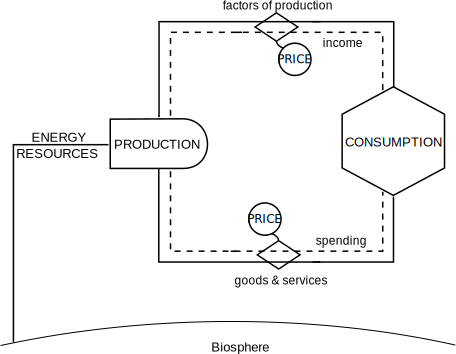
\includegraphics[width=\linewidth]{Part_0/Chapter_Introduction/images/Perpetual_motion_2.pdf}
\caption[The machine model]{The machine model of the economy includes
flows of energy into the economy from the biosphere.
This may be considered a perpetual motion machine 
of the second kind.}
\label{fig:perp_motion_2}
\end{figure}

The machine metaphor and engine model are still very much mechanistic.
Much like the engines of the Industrial Revolution,
the economic engine is assumed to be well-behaved and amenable to control.
Even today, machine metaphors abound in our economic discussions.
We speak of ``fueling'' the ``economic engine'' 
lest it should ``stall.''~\cite{Liu2012}
Like a well-running engine, the economy is assumed 
to be resilient to small or even quite large perturbations.  
It can either self-correct, 
or be corrected with adjustments to
a few predictable policy levers.

But, in light of the challenges discussed above,
how accurate is the engine model?

According to the Second Law of Thermodynamics,
all real-world processes involve the degradation
of material and especially energy resources
and the creation of entropy.
High quality (low entropy) material and energy come in;
low quality (high entropy) material and energy go out.
The depiction in Figure~\ref{fig:perp_motion_2} 
can be classified as a perpetual motion machine
of the \emph{second kind}:
it perfectly converts energy resources into 
work~(useful services) without generating
any entropy,
in violation of the Second Law of Thermodynamics.
Because the generation of high entropy~(low quality)
output is a \emph{necessary} feature of \emph{all} processes 
(including economic processes)
then the generation of wastes is a \emph{normal} feature of
economic processes,
not an anomaly.
Within a closed system, such as the earth,
these wastes soon accumulate,
necessitating the change to a ``spaceship'' economy,
wherein account is made of the waste outflows from
the economy.

We need a different model.


%%%%%%%%%% A new metaphor %%%%%%%%%%
\subsection{A new metaphor}
\label{sec:new_metaphor}
%%%%%%%%%% 

When our collective imagination is stuck on a metaphor that 
informs models in which the economy is isolated from or closed to the biosphere,
the suggestion to ``account for the environment'' is unconvincing, and 
the challenges cited earlier (natural resource extraction limits,
difficulty of material and energy substitutions, and 
exceeding the biosphere's waste assimilation capacity)
seem unimportant. 

Mounting evidence shows otherwise.

Thus, we need to find a new way to understand the complex, 
messy dynamics of real-world economies;
we need a new way to make sense of real-world events;
we need a new way to learn where and how economies can go wrong; and
we need to plan for the impending materials and energy transformations.
To do so, we had better be counting data to assess \emph{dynamic} models
guided by metaphors that tell us \emph{more} than ``the world is an orderly place.''
Our counting needs to be informed by metaphors and models that are
able to cope with rapid transience and transformation,
not just ordered stability.

We need a new metaphor.


%%%%%%%%%% An Apt Metaphor %%%%%%%%%%
\section{An apt metaphor for the economy}
\label{sec:apt_metaphor}
%%%%%%%%%%

If the clockwork and machine metaphors are unsuitable, 
what might an apt metaphor for the economy be?
And, if we find an apt metaphor, what types of models would it inform?
Furthermore, what data would the models tell us to collect?
That is, how should we go about accounting for the environment?
From here to Section~\ref{sec:our_new_model}, we answer the above questions
and, in the process, sketch the outline of our new approach 
to thinking about and accounting for materials, energy, and the economy.
Later chapters will flesh out this sketch.

To begin the search for an apt metaphor, 
we might first ask the question, 
what characteristics should the metaphor possess?
In our opinion, an apt metaphor should account for the facts 
that a real economy:

\begin{enumerate}
	\item{\label{itm:intake}intakes material and energy from the biosphere}
	\item{\label{itm:internal_exchange}exchanges materials, energy, and information internally}
	\item{\label{itm:discharge}discharges material and energy wastes to the biosphere}
	\item{\label{itm:energetic_costs}is affected by energetic costs}
	\item{\label{itm:scarcity}is affected non-linearly by scarcity 
			in the face of low substitutibility}
	\item{\label{itm:non-linear}can change non-linearly or in discrete steps with the potential 
			for structural transformation}
	\item{\label{itm:embodies}embodies energy in material stocks, and}
	\item{\label{itm:robust}maintains organizational structure despite changes 
			in the environment.\footnote{We note that 
				several areas of the literature speak to the items in this list.
				Material Flow Analysis~(MFA) and 
				Economy-Wide Material Flow Analys~(EW-MFA)
				stress the importance of
				material intake by the economy. 
				(See Section~\ref{sec:materials_auto}.)
				The Input-Output~(I-O) method highlights the effects of internal exchanges
				of material and information with economies. 
				(See Chapter~\ref{chap:intensity}.)
				Life-Cycle Assessment~(LCA) techniques focus attention 
				on otherwise-neglected wastes. 
				(See Section~\ref{sec:intensity_auto}.)
				Net Energy Analysis~(NEA) predicts that energy resource 
				scarcity reduces Energy Return on Investment~(EROI)
				and increases energy prices.
				(See Sections~\ref{sec:B_energy} 
				and~\ref{sec:resource_quality_and_irreversibility}.)
				The Energy Input-Output~(EI-O) method gives prominence to energetic costs
				for internal material and energy flows.
				(See Chapter~\ref{chap:intensity}.)
				And, thermodynamic control-volume modeling describes
				transient behavior and system transformations.
				(See Chapters~\ref{chap:materials}--\ref{chap:value}.)
			}}
\end{enumerate}

Living metabolisms\footnote{The 
	Greek root of metabolism 
	(\emph{metabol$\bar{e}$}) means ``change.''}
exhibit the characteristics in the list above.
Metabolisms and the organisms they support
are intimately connected with the biosphere:
they withdraw materials and energy from the biosphere~(\ref{itm:intake}), 
transfer materials and energy internally via metabolic processes~(\ref{itm:internal_exchange}),
and discharge wastes back to the biosphere~(\ref{itm:discharge});
in fact, their very survival depends on these processes.
Extending Figures~\ref{fig:perp_motion_1} and~\ref{fig:perp_motion_2}
to include the facts in items~(\ref{itm:intake})--(\ref{itm:discharge}), % chktex 36
we obtain Figure~\ref{fig:metabolic_economy}.
Metabolisms are affected by energetic costs~(\ref{itm:energetic_costs}): 
an organism that obtains less energy than it expends is doomed.
Withholding life-sustaining resources brings drastic, non-linear
consequences for any metabolism~(\ref{itm:scarcity}).
Metabolisms enable non-linear, structural transformations
in their host organisms (e.g., metamorphosis, puberty, and evolution)~(\ref{itm:non-linear}).
And, energy absorbed into a metabolism is considered to be ``embodied''
in the cells of the organism~(\ref{itm:embodies}).
Metabolisms exist in a state of dynamic stability~(\ref{itm:robust}),
adjusting and readjusting to maintain their internal conditions
despite changes in the environment;
for a metabolism, equilibrium means death!

The economy is society's metabolism.\cite{F-K1998, Giampietro2000, Giampietro2013}

\begin{figure}[!ht]
\centering\
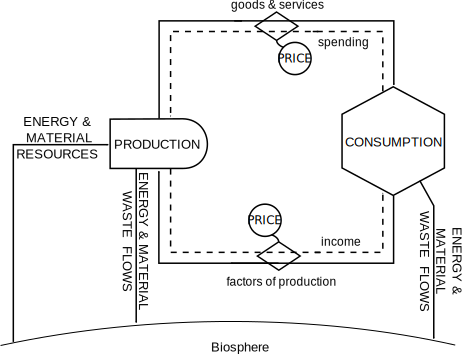
\includegraphics[width=\linewidth]{Part_0/Chapter_Introduction/images/PERKS.pdf}
\caption[The metabolism model]{The metabolism model provides a comprehensive view 
of the economy, fully consistent with the laws of thermodynamics, 
including degraded resources (waste) expelled 
to the environment as a necessary consequence of economic activity.}
\label{fig:metabolic_economy}
\end{figure}


%%%%%%%%%% Apt Models %%%%%%%%%%
\section{An apt material, energy, and economy model}
\label{sec:apt_models}
%%%%%%%%%%

As discussed in Section~\ref{sec:metaphors_and_models}, 
metaphors give rise to models.
So, a natural question is: 
``what types of models does the metabolism metaphor inform?''

In our opinion, apt models should have the following characteristics:

\begin{enumerate}
	\item{\label{itm:flows}account for flows of materials and energy 
			into, within, and out of the economy,}
	\item{\label{itm:accumulation}account for accumulation of materials and energy 
			within the economy,}
	\item{\label{itm:metrics}provide metrics that relate energy demands and economic value, and}
	\item{\label{itm:accounting}provide results that are comparable against existing 
			(or expanded) national accounting.}
\end{enumerate}

Material and energy flow balance equations, 
often employed by thermodynamicists, 
can account for both flows~(\ref{itm:flows}) and accumulation~(\ref{itm:accumulation}) 
of materials and energy within systems.
We will adapt an existing Input-Output~(I-O)
energy analysis method to develop a 
technique for obtaining metrics 
of energy and economic value~(\ref{itm:metrics}).\footnote{See Chapter~\ref{chap:intensity}
for details of the I-O method.}
Finally, we note that systems of national accounts use the economic sector
as their level of analysis. 
Thus, apt models should be also implemented at the economic sector level
so that model results can be 
compared against existing (or expanded) national accounting~(\ref{itm:accounting}).


%%%%%%%%%% Our new model %%%%%%%%%%
\section{Our new model}
\label{sec:our_new_model}
%%%%%%%%%%

%**** Add a discussion of the "system" and "boundaries". Discuss levels of disaggregation as a proxy for area of interest ****
%
%**** Emphasize the greater understanding that comes from explicitly modeling accumulation of (embodied) energy and materials within the economy. ****
%
%**** You have to draw boundaries somewhere.****
%
%**** We disaggregate the economy, because that the is the locus of our interest. An ecologist, in contrast, may choose to disaggregated the biosphere to answer questions such as biodiversity, etc. The biosphere is a container with which our system of interest is interacting. Why? An area of interest is the impact of energy transitions on the economy. ****

We contend that society is not accounting materials and energy adequately 
to prepare for the coming material and energy transformations 
**** MCD - metamorphosis? ****.
In Sections~\ref{sec:apt_metaphor} and~\ref{sec:apt_models} above,
we identified a metabolism as an apt metaphor and model for the economy 
to assist the process of developing the knowledge and analysis approaches
necessary to plan for the upcoming transitions.
Some elements of our approach are not new.
We're not the first to claim that a metabolism is an apt metaphor for the economy
(Section~\ref{sec:apt_metaphor}).~\cite{Barradas1936, F-K1998, Giampietro2000, Haberl2001, Daniels2001}
Nor are we the first to claim that an apt model for the economy 
involves material and energy flow equations 
applied at the level of economic sectors using an Input-Output framework.~\cite{G-R1975 ,G-R1979a, Lenzen1998, Hendrickson2006}

But, we are the first to comprehensively include accumulation
of materials and embodied energy in an accounting framework
based on existing systems of national accounts.
We contend that accounting for accumulation 
of materials and embodied energy in economic sectors is essential
for several reasons:

**** Mik, can you have a look at this list? Matt ****

\begin{itemize}
	\item{real economies convert raw materials extracted from the biosphere
		 	into engineered objects that accumulate,  
			embodied as the infrastructure of the economy;}
	\item{accumulated materials and infrastructure require further material and energy flows
			for their operation and maintenance,
			thereby placing additional material and energy demands on the biosphere;}
	\item{accumulated materials and infrastructure depreciate and need to be replaced,
		 	leading to additional material and energy demands on the biosphere,}
	\item{rapidly growing economies have large accumulation rates, 
			and accounting only for non-accumulating,
			consumptive (through-put) flows of material and energy 
			underestimates the energy demands of those economies.}
\end{itemize}

To include this accumulation of materials and embodied energy, 
we had to re-think the I-O framework starting from fundamental assumptions
and then re-derive the I-O accounting equations
to allow for accumulation, as shown in the following chapters. 
Thus, to our knowledge, we are the first 
to systematically derive the I-O equations to account for accumulation
in a thermodynamically-consistent manner.

To complete the outline and scope for our new model, 
the following subsections address
questions of system boundary and what must be counted.


%%%%%%%%%% System boundary %%%%%%%%%%
\subsection{System boundary}
\label{sec:system_boundary}
%%%%%%%%%% 

In Figure~\ref{fig:biosphere_economy},
the economy is shown as embedded within the surrounding environment,
the biosphere.
Materials and energy (yellow arrows) flow around the biosphere,
many of which do not interact with the economy.
Some of the flows are extracted from the biosphere for human purposes.
These flow around (and accumulate within) the economy,
before ultimately being emitted back into the biosphere as waste.
Processes within the biosphere are then able to regenerate some of these
flows making them available again for human use,
for example the conversion of carbon dioxide into oxygen by photosynthesis.

We have chosen to draw the system boundary of this new model around the economy
and focus only on those flows that pass through the economy.\footnote{An ecologist
	is likely have a different focus 
	and study material and energy flows that never enter the economy.
	}
This is the same system boundary used by the
systems of national accounts (SNA),
although the types of flows accounted are different.
As will be seen in later chapters,
the economy (as our main locus of interest) is further disaggregated 
to the level of industrial sectors.
Our primary interest in doing this is that it is important 
to know where materials and energy accumulate in understanding
the structure of our economies.
This will provide us a better model of the economy and
enable greater understanding of the structural transformation that lies ahead.

The biosphere is included in the model, but only at an aggregated level;
it is the container for the economy. 
We ignore material and energy flows that occur only within the biosphere,
but do not enter the economy.
This means that many important issues lie outside the scope of our new model. 
For example, questions of species loss and
bio-diversity remain outside of this system. 

**** MCD - WHICH VERSION OF THE FIGURE DO WE PREFER?? ****


\begin{figure}[!ht]
\centering\
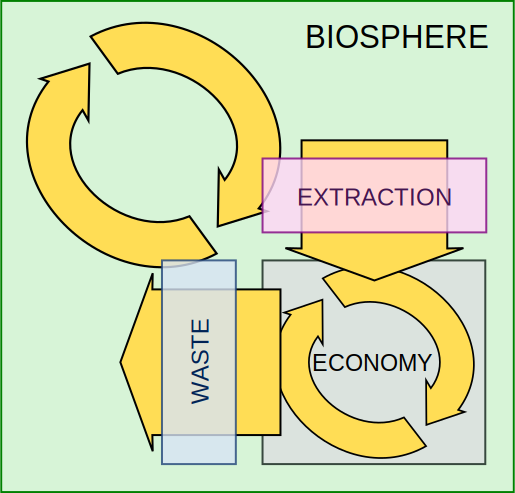
\includegraphics[width=\linewidth]{Part_0/Chapter_Introduction/images/Biosphere_economy.pdf}
\caption[The biosphere and the economy **** MCD - NEED A BETTER FIGURE TITLE ****]
				{The interaction of the economy with the biosphere.
				Materials and energy (yellow arrows) flow around the biosphere.
				Some flows are extracted for human use and enter the economy.
				The materials and energy flow around the economy 
				(as well as accumulating in capital stocks)
				before being emitted as wastes back into the biosphere.
				The size of the arrows does not indicate magnitude of flows.}
\label{fig:biosphere_economy}
\end{figure}

\begin{figure}[!ht]
\centering\
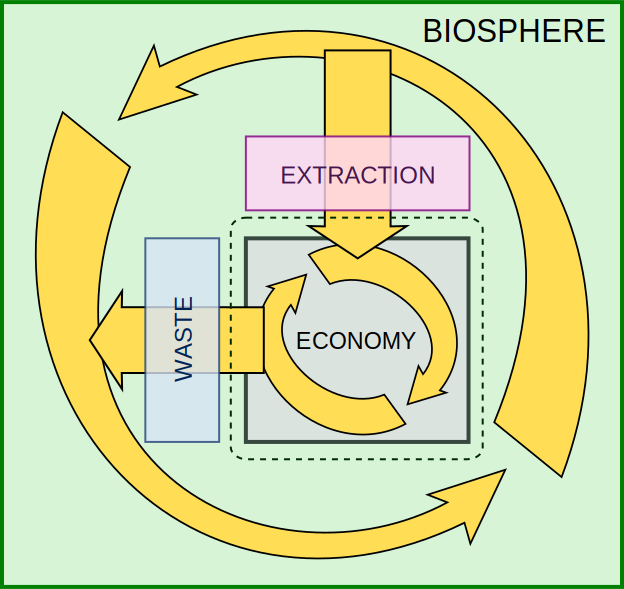
\includegraphics[width=\linewidth]{Part_0/Chapter_Introduction/images/Biosphere_economy_v2.pdf}
\caption[The biosphere and the economy **** MCD - NEED A BETTER FIGURE TITLE ****]
				{The interaction of the economy with the biosphere.
				Materials and energy (yellow arrows) flow around the biosphere.
				Some flows are extracted for human use and enter the economy.
				The materials and energy flow around the economy 
				(as well as accumulating in capital stocks)
				before being emitted as wastes back into the biosphere.
				The size of the arrows does not indicate magnitude of flows.}
\label{fig:biosphere_economy}
\end{figure}


%%%%%%%%%% What to count %%%%%%%%%%
\subsection{What to count}
\label{sec:what_to_count}
%%%%%%%%%% 

We believe the key to understanding how energy transformations will unfold
involves specifically understanding how

\begin{itemize}
	\item{materials,}
	\item{energy,}
	\item{embodied energy, and}
	\item{economic value}
\end{itemize}

\noindent{}each flow and accumulate within society's metabolism, the economy.
Of course, each of the above items interacts with the others 
and the biosphere dynamically.
If we can begin to carefully track these items, 
we will be on our way to gathering the information required to 
assist planning for upcoming materials and energy transformations.

A model informed by the metabolism metaphor may allow consumers, producers,
and policy-makers to answer critical questions that are not
answerable today. Example questions include:

\begin{enumerate}
	\item{What might be the optimal scale of an economy in terms of GDP 
			and what are the impacts of an optimally-sized economy on natural capital?}
    \item{How is fossil fuel dependency embedded in the interlocking fabric of the economy?} 
    \item{How will economies that are dependent on coal, oil, 
 			and other forms of non-renewable energy transition 
			to renewable forms of energy?}
	\item{How might an economy be affected as an increasing share of production
			is directed toward replacing 
			degraded ecosystem services?~\cite[p.~221]{kummel2011}​}
\end{enumerate}

To summarize Sections~\ref{sec:apt_metaphor}--\ref{sec:what_to_count}, 
our approach is to:

\begin{svgraybox}
	develop a dynamic model 
	by applying rigorous thermodynamics 
	to materials and energy flows into, among, 
	and out of economic sectors,
	informed by the metabolism metaphor,
	in a manner that is verifiable against 
	the existing (or expanded) 
	national accounts.
\end{svgraybox}

\noindent{}If successful, we will have developed an analysis framework 
that allows us to \emph{account for the environment}.


%%%%%%%%%% Structure %%%%%%%%%%
\section{Structure of the book}
\label{sec:structure}
%%%%%%%%%%

The bulleted list in Section~\ref{sec:what_to_count} 
provides the beginning of the structure for the rest of this book.

Part~\ref{part:matter} addresses flows of physical matter and energy
through the economy.
Chapter~\ref{chap:materials} discusses material flows and accumulation.
Flows of energy are covered in Chapter~\ref{chap:direct_energy}, 
and a rigorous, thermodynamics-based definition of and accounting for 
embodied energy is presented in Chapter~\ref{chap:embodied_energy}.

In Part~\ref{part:values}, we turn to flow and accumulation of 
non-physical entities through the economy. 
Flows and accumulation of economic value are discussed in Chapter~\ref{chap:value}.
In Chapter~\ref{chap:intensity}, we combine the results from 
Chapters~\ref{chap:embodied_energy} and~\ref{chap:value} to
calculate an important indicator of economic activity:
the energy intensity of economic production.

Part~\ref{part:implications} gives context to the framework developed in
Parts~\ref{part:matter}~and~\ref{part:values}.
Chapter~\ref{chap:implications} draws out some of the direct implications
of our framework.
Chapter~\ref{chap:unfinished_business} looks at 
unfinished business: practical, conceptual, and theoretical issues
that arise in the development of this framework.
And, we end with a summary in Chapter~\ref{chap:summary}.

\begin{table}
\caption[Examples used throughout this book]{Examples
used throughout this book.}
\begin{center}
  \begin{tabular}{c @{\hspace{1.5em}} c @{\hspace{1.5em}} c @{\hspace{1.5em}} c @{\hspace{1.5em}} c}
    \toprule
    Example & Sector 0 & Sector 1 & Sector 2 & Sector 3 \\ 
	\midrule
    A & Biosphere	&	Society            & NA         & NA                 \\
    B & Biosphere	&	Final Consumption  & Production & NA                 \\
    C & Biosphere	&	Final Consumption  & Energy     & Goods \& Services  \\
  \bottomrule
  \end{tabular}
\end{center}
\label{tab:examplesABC}
\end{table}
 
Throughout the methodological chapters~(\ref{chap:materials}--\ref{chap:intensity}),
our accounting framework is developed
through a series of increasingly-disaggregated
models of the economy~(Table~\ref{tab:examplesABC}),
and we use the US auto industry 
as a running example for application and discussion.

**** The next two paragraphs are duplicated from 
Section 2.5 (Materials in the US Auto Industry).
We duplicated them here temporarily so that the editors can 
see the purpose of and justification for the auto industry example. ****

The running example of the US auto industry demonstrates that our dynamic model 
can be tied into national accounts.
The US auto industry example shows where data are available 
(e.g., economic value, Chapter~\ref{chap:value}), 
where it is old (e.g., energy intensity, Chapter~\ref{chap:intensity}), 
and where it has never been available 
(e.g., accumulated embodied energy, Chapter~\ref{chap:embodied_energy}).  
The US auto industry is, therefore, 
illustrative of the challenges inherent 
in obtaining data that would feed the model.

The auto industry 
has been used previously
in the literature in both 
process-based~\cite{Berry:1973vo, Sullivan1995, Stodolsky1995, 
							Sullivan1998, McCleese2002, Sullivan2010, Hawkins2012}
and Input-Output~\cite{Bullard:1978vd, MacLean1998, MacLean2003}
analysis methods,
Furthermore, the industry
remains a large portion of many industrialized economies, 
is very resource intensive, 
has obvious links with energy because
its health is sensitive to disruptions in energy supplies, and
the industry also shows evidence of 
post-industrial decline (shrinking profit margins, etc.).

\bibliographystyle{unsrt}
\bibliography{../../Metabolic}


% Always give a unique label
% and use \ref{<label>} for cross-references
% and \cite{<label>} for bibliographic references
% use \sectionmark{}
% to alter or adjust the section heading in the running head
%% Instead of simply listing headings of different levels we recommend to let every heading be followed by at least a short passage of text. Furtheron please use the \LaTeX\ automatism for all your cross-references and citations.

%% Please note that the first line of text that follows a heading is not indented, whereas the first lines of all sequent paragraphs are.

%% Use the standard \verb|equation| environment to typeset your equations, e.g.
%
%% \begin{equation}
%% a \times b = c\;,
%% \end{equation}
%
%% however, for multiline equations we recommend to use the \verb|eqnarray|
%% environment\footnote{In physics texts please activate the class option \texttt{vecphys} to depict your vectors in \textbf{\itshape boldface-italic} type - as is customary for a wide range of physical jects.}.
%% \begin{eqnarray}
%% a \times b = c \nonumber\\
%% \vec{a} \cdot \vec{b}=\vec{c}
%% \label{eq:01}
%% \end{eqnarray}

%% \section{section Heading}
%% \label{sec:2}
%% Instead of simply listing headings of different levels we recommend to let every heading be followed by at least a short passage of text. Furtheron please use the \LaTeX\ automatism for all your cross-references\index{cross-references} and citations\index{citations} as has already been described in Sect.~\ref{sec:2}.

%% \begin{quotation}
%% Please do not use quotation marks when quoting texts! Simply use the \verb|quotation| environment -- it will automatically render Springer's preferred layout.
%% \end{quotation}


%% \section{section Heading}
%% Instead of simply listing headings of different levels we recommend to let every heading be followed by at least a short passage of text. Furtheron please use the \LaTeX\ automatism for all your cross-references and citations as has already been described in Sect.~\ref{sec:2}, see also Fig.~\ref{fig:1}\footnote{If you copy text passages, figures, or tables from other works, you must obtain \textit{permission} from the copyright holder (usually the original publisher). Please enclose the signed permission with the manucript. The sources\index{permission to print} must be acknowledged either in the captions, as footnotes or in a separate section of the book.}

%% Please note that the first line of text that follows a heading is not indented, whereas the first lines of all sequent paragraphs are.

% For figures use
%
%% \begin{figure}[b]
%% \sidecaption
% Use the relevant command for your figure-insertion program
% to insert the figure file.
% For example, with the option graphics use
%% \includegraphics[scale=.65]{figure}
%
% If not, use
%\picplace{5cm}{2cm} % Give the correct figure height and width in cm
%
%% \caption{If the width of the figure is less than 7.8 cm use the \texttt{sidecapion} command to flush the caption on the left side of the page. If the figure is positioned at the top of the page, align the sidecaption with the top of the figure -- to achieve this you simply need to use the optional argument \texttt{[t]} with the \texttt{sidecaption} command}
%% \label{fig:1}       % Give a unique label
%% \end{figure}


%% \paragraph{Paragraph Heading} %
%% Instead of simply listing headings of different levels we recommend to let every heading be followed by at least a short passage of text. Furtheron please use the \LaTeX\ automatism for all your cross-references and citations as has already been described in Sect.~\ref{sec:2}.

%% Please note that the first line of text that follows a heading is not indented, whereas the first lines of all sequent paragraphs are.

%% For typesetting numbered lists we recommend to use the \verb|enumerate| environment -- it will automatically render Springer's preferred layout.

%% \begin{enumerate}
%% \item{Livelihood and survival mobility are oftentimes coutcomes of uneven socioeconomic development.}
%% \begin{enumerate}
%% \item{Livelihood and survival mobility are oftentimes coutcomes of uneven socioeconomic development.}
%% \item{Livelihood and survival mobility are oftentimes coutcomes of uneven socioeconomic development.}
%% \end{enumerate}
%% \item{Livelihood and survival mobility are oftentimes coutcomes of uneven socioeconomic development.}
%% \end{enumerate}


%% \paragraph{paragraph Heading} In order to avoid simply listing headings of different levels we recommend to let every heading be followed by at least a short passage of text. Use the \LaTeX\ automatism for all your cross-references and citations as has already been described in Sect.~\ref{sec:2}, see also Fig.~\ref{fig:2}.

%% Please note that the first line of text that follows a heading is not indented, whereas the first lines of all sequent paragraphs are.

%% For unnumbered list we recommend to use the \verb|itemize| environment -- it will automatically render Springer's preferred layout.

%% \begin{itemize}
%% \item{Livelihood and survival mobility are oftentimes coutcomes of uneven socioeconomic development, cf. Table~\ref{tab:1}.}
%% \begin{itemize}
%% \item{Livelihood and survival mobility are oftentimes coutcomes of uneven socioeconomic development.}
%% \item{Livelihood and survival mobility are oftentimes coutcomes of uneven socioeconomic development.}
%% \end{itemize}
%% \item{Livelihood and survival mobility are oftentimes coutcomes of uneven socioeconomic development.}
%% \end{itemize}

%% \begin{figure}[t]
%% \sidecaption[t]
% Use the relevant command for your figure-insertion program
% to insert the figure file.
% For example, with the option graphics use
%% \includegraphics[scale=.65]{figure}
%
% If not, use
%\picplace{5cm}{2cm} % Give the correct figure height and width in cm
%
%% \caption{Please write your figure caption here}
%% \label{fig:2}       % Give a unique label
%% \end{figure}

%% \runinhead{Run-in Heading Boldface Version} Use the \LaTeX\ automatism for all your cross-references and citations as has already been described in Sect.~\ref{sec:2}.

%% \runinhead{Run-in Heading Italic Version} Use the \LaTeX\ automatism for all your cross-refer\-ences and citations as has already been described in Sect.~\ref{sec:2}\index{paragraph}.
% Use the \index{} command to code your index words
%
% For tables use
%
%% \begin{table}
%% \caption{Please write your table caption here}
%% \label{tab:1}       % Give a unique label
%
% For LaTeX tables use
%
%% \begin{tabular}{p{2cm}p{2.4cm}p{2cm}p{4.9cm}}
%% \hline\noalign{\smallskip}
%% Classes & class & Length & Action Mechanism  \\
%% \noalign{\smallskip}\svhline\noalign{\smallskip}
%% Translation & mRNA$^a$  & 22 (19--25) & Translation repression, mRNA cleavage\\
%% Translation & mRNA cleavage & 21 & mRNA cleavage\\
%% Translation & mRNA  & 21--22 & mRNA cleavage\\
%%Translation & mRNA  & 24--26 & Histone and DNA Modification\\
%%\noalign{\smallskip}\hline\noalign{\smallskip}
%%\end{tabular}
%%$^a$ Table foot note (with superscript)
%%\end{table}
%
%% \section{Section Heading}
%%\label{sec:3}
% Always give a unique label
% and use \ref{<label>} for cross-references
% and \cite{<label>} for bibliographic references
% use \sectionmark{}
% to alter or adjust the section heading in the running head
%% Instead of simply listing headings of different levels we recommend to let every heading be followed by at least a short passage of text. Furtheron please use the \LaTeX\ automatism for all your cross-references and citations as has already been described in Sect.~\ref{sec:2}.

%% Please note that the first line of text that follows a heading is not indented, whereas the first lines of all sequent paragraphs are.

%%If you want to list definitions or the like we recommend to use the Springer-enhanced \verb|description| environment -- it will automatically render Springer's preferred layout.

%%\begin{description}[Type 1]
%%\item[Type 1]{That addresses central themes pertainng to migration, health, and disease. In Sect.~\ref{sec:1}, Wilson discusses the role of human migration in infectious disease distributions and patterns.}
%%\item[Type 2]{That addresses central themes pertainng to migration, health, and disease. In Sect.~\ref{sec:2}, Wilson discusses the role of human migration in infectious disease distributions and patterns.}
%%\end{description}

%%\section{section Heading} %
%% In order to avoid simply listing headings of different levels we recommend to let every heading be followed by at least a short passage of text. Use the \LaTeX\ automatism for all your cross-references and citations citations as has already been described in Sect.~\ref{sec:2}.

%% Please note that the first line of text that follows a heading is not indented, whereas the first lines of all sequent paragraphs are.

%% \begin{svgraybox}
%% If you want to emphasize complete paragraphs of texts we recommend to use the newly defined Springer class option \verb|graybox| and the newly defined environment \verb|svgraybox|. This will produce a 15 percent screened box 'behind' your text.

%% If you want to emphasize complete paragraphs of texts we recommend to use the newly defined Springer class option and environment \verb|svgraybox|. This will produce a 15 percent screened box 'behind' your text.
%% \end{svgraybox}


%% \section{section Heading}
%%Instead of simply listing headings of different levels we recommend to let every heading be followed by at least a short passage of text. Furtheron please use the \LaTeX\ automatism for all your cross-references and citations as has already been described in Sect.~\ref{sec:2}.

%% Please note that the first line of text that follows a heading is not indented, whereas the first lines of all sequent paragraphs are.

%% \begin{theorem}
%% Theorem text goes here.
%% \end{theorem}
%
% or
%
%% \begin{definition}
%% Definition text goes here.
%% \end{definition}

%% \begin{proof}
%\smartqed
%% Proof text goes here.
%% \qed
%% \end{proof}

%%\paragraph{Paragraph Heading} %
%% Instead of simply listing headings of different levels we recommend to let every heading be followed by at least a short passage of text. Furtheron please use the \LaTeX\ automatism for all your cross-references and citations as has already been described in Sect.~\ref{sec:2}.

%% Note that the first line of text that follows a heading is not indented, whereas the first lines of all subsequent paragraphs are.
%
% For built-in environments use
%
%%\begin{theorem}
%%Theorem text goes here.
%%\end{theorem}
%
%%\begin{definition}
%%Definition text goes here.
%%\end{definition}
%
%%\begin{proof}
%%\smartqed
%% Proof text goes here.
%%\qed
%%\end{proof}
%
%% \begin{acknowledgement}
%% If you want to include acknowledgments of assistance and the like at the end of an individual chapter please use the \verb|acknowledgement| environment -- it will automatically render Springer's preferred layout.
%% \end{acknowledgement}
%
%% \section*{Appendix}
%% \addcontentsline{toc}{section}{Appendix}
%
%% When placed at the end of a chapter or contribution (as opposed to at the end of the book), the numbering of tables, figures, and equations in the appendix section continues on from that in the main text. Hence please \textit{do not} use the \verb|appendix| command when writing an appendix at the end of your chapter or contribution. If there is only one the appendix is designated ``Appendix'', or ``Appendix 1'', or ``Appendix 2'', etc. if there is more than one.

%% \begin{equation}
%% a \times b = c
%% \end{equation}
% Problems or Exercises should be sorted chapterwise
%% \section*{Problems}
%% \addcontentsline{toc}{section}{Problems}
%
% Use the following environment.
% Don't forget to label each problem;
% the label is needed for the solutions' environment
%% \begin{prob}
%% \label{prob1}
%% A given problem or Excercise is described here. The
%% problem is described here. The problem is described here.
%% \end{prob}

%% \begin{prob}
%% \label{prob2}
%% \textbf{Problem Heading}\\
%% (a) The first part of the problem is described here.\\
%% (b) The second part of the problem is described here.
%% \end{prob}




\part{Material and Energy Flows}
\label{part:matter}

%!TEX root = ../../Heun_Dale_Haney_A_dynamic_approach_to_input_output_modeling.tex
%%%%%%%%%%%%%%%%%%%%% chapter.tex %%%%%%%%%%%%%%%%%%%%%%%%%%%%%%%%%
%
% sample chapter
%
% Use this file as a template for your own input.
%
%%%%%%%%%%%%%%%%%%%%%%%% Springer-Verlag %%%%%%%%%%%%%%%%%%%%%%%%%%
%\motto{Use the template \emph{chapter.tex} to style the various elements of your chapter content.}
\chapter{Material flows}
% use \chaptermark{}
% to alter or adjust the chapter heading in the running head
\chaptermark{Materials}
% Always give a unique label
\label{chap:materials} 

\abstract*{[NEED TO ADD ABSTRACT HERE]}

%% \abstract{Each chapter should be preceded by an abstract (10--15 lines long) that summarizes the content. The abstract will appear \textit{online} at \url{www.SpringerLink.com} and be available with unrestricted access. This allows unregistered users to read the abstract as a teaser for the complete chapter. As a general rule the abstracts will not appear in the printed version of your book unless it is the style of your particular book or that of the series to which your book belongs.\newline\indent
%% Please use the 'starred' version of the new Springer \texttt{abstract} command for typesetting the text of the online abstracts (cf. source file of this chapter template \texttt{abstract}) and include them with the source files of your manuscript. Use the plain \texttt{abstract} command if the abstract is also to appear in the printed version of the book.}

%% Use the template \emph{chapter.tex} together with the Springer document class SVMono (monograph-type books) or SVMult (edited books) to style the various elements of your chapter content in the Springer layout.

In the Introduction, we introduced the idea that economies are like organisms. 
This chapter explores
this idea further by observing the interchange of materials \emph{within}
an economy, as well as exchanges of materials between an economy and 
surrounding environment---the biosphere. 

% [THE FOLLOWING PARAGRAPH CONNECTS MORE WITH THE METABOLISM METAPHOR,
% NEED TO DECIDE BETWEEN THAT AND THE ONE AFTER OR MAYBE MIX THE TWO]

% Just as a living organism takes
% in food, water and air, so too an
% economy must take in raw materials from its environment. To a large extent,
% the major exchanges of materials between industrial economies and their 
% environment mirror those of an animal. Large inputs of fresh water, hydrocarbons
% and oxygen with the emission of carbon dioxide and polluted water [REF BRANDT]
% dioxide and hydro-carbons These
% materials are then used for a number of different purposes. Some
% become the building blocks from which the physical structures within the 
% economy---buildings, roads, even people---are composed. These materials
% must be extracted from the environment and processed, transported and then
% manufactured into final goods. Such activities require energy resources. In
% an economy primarily dependent on the combustion of fossil fuels, energy conversion
% of energy necessarily requires the presence of oxygen in the atmosphere and
% the emission of carbon dioxide. Many processes also require flows of materials, 
% especially fresh water, that are not directly embodied in the final product.
 

There are many easily observable instances of material flow within an
economy. I look around my office at my computer screen and coffee cup
and myriad other items. I look out my window to the street and building
opposite. All of these goods came originally from natural resources, be it paper or
petroleum or rock. They were extracted and processed, transported and
transformed requiring yet more materials and energy inputs in the form of
electricity or fuels. 

There are also inumerable material flows caused by an economy that we do not observe.
The extraction of raw materials generates additional overburden---earth that must be
extracted and processed and ultimately discarded without ever entering the economy
proper. Other flows occur around us unseen. The cars outside my window suck in nitrogen
and oxygen (without which the engine would not work) and emit water, carbon dioxide and
other more harmful substances. 

Even services which we tend to think of as non-material, require at least some material
infrastructure. The hairdresser requires scissors (and to a greater or lesser extent 
some hair) with which to work. Even the internet, often lauded as the exemplar of
dematerialization of the economic process, requires a whole host of computer
infrastructure including electricity, data servers, telephone networks and a
computer by which to access it.

In this chapter, we will define a mathematical framework by which to track the flow of
materials within an economy, building from a one-sector economy up to examples of both a
two- and three-sector economy. We will finally apply this framework to the illustrative
example of the US automobile industry that runs through the whole book. First let us
outline the basic methodology.

\section{Methodology}
\label{sec:Materials_Methodology}

% Everyone is familiar with the notion of accounting of material (and even non-material)
% things. In order to be rigorous, the first step requires the definition of what we
% will be counting as well as the place (defined in both time and space) for which we will
% be counting. Engineers often call this a \emph{control volume}. For example, I may wish
% to account the number of apples in my home over a week-long period. In which case,
% I would count the number of apples that enter  and leave my home, as well as any apples
% that are eaten and, just in case I happen to have an apple tree, any apples that grow
% inside my home. Our accounting equation would look something like:

%**** The idea that we are "counting money" does not seem exactly 
%right to me. Isn't it that we are accounting for value and energy flows? 
%Later on we will use currency flows to approximate the value flows? BRH ****


This book is about tracking (accounting) flows through the 
economy with a focus on counting materials, energy and value.
That an entire academic discipline and industry are focused on counting money (accounting)
is evidence of its importance in today's economies.
That energy is required to do \emph{anything} is evidence 
of its importance in the economic activity of our daily lives.
And, we believe that the interplay between money and energy
has shaped the past and will continue to influence the future.
In this section, we define rigorous ``counting'' methods that will be applied
to money and energy throughout this book.

Everyone counts material (and even non-material) things. 
Rigorous counting requires precise definition of both 
what we will be counting
and the place (defined in both time and space) in which we will be counting. 
Engineers often call this definition a ``control volume.'' Another way to think of
control volume is drawing a boundary. What gets counted is 
what passes through the boundary.
For example, I may wish to count (or ``make an accounting of") 
what happens to the stock  of apples in my home over a week-long period. 
I've drawn a boundary around my home and around a week-long time period.
I  count the apples that enter and leave my home, 
apples that are eaten (consumed),
and, if I own an apple tree, apples that I grow (produce) during a week. 
A rigorous apple accounting equation is:

\begin{equation}
	\Delta\textrm{apples} 
	= \textrm{apples in} 
	- \textrm{apples out} 
	+ \textrm{apples grown} 
	- \textrm{apples eaten}.
\end{equation}

\noindent More generally, we may say:

\begin{equation}
	\textrm{Accumulation}
	= \textrm{Transfers in} 
	- \textrm{Transfers out}
	+ \textrm{Production}
	- \textrm{Consumption}.
\end{equation}

Notice that, when discussing apples we use the specific terms, ``grown'' and
``eaten'' instead of the more general terms, ``produced'' and ``consumed''.
Later, in Chapter \ref{chap:value}, when discussing value, we will use the terms
``generated'' and ``destroyed''. In reality, these terms all have the equivalent
sets of meaning and we use them inter-changeably.

Once I account for how much the stock of apples changes in a weekly period,
I can reframe my question to ask, "how fast does the stock of
apples change." That is, I can examine the rate of
change of the apple stock per time unit in relation to the flow of apples per time unit ($\dot{a}$), 
e.g. in units of apples per day, 
in which case our accounting equation would become:

\begin{equation} \label{eq:apple_rate_accounting}
	\frac{\mathrm{d}a}{\mathrm{d}t}
	= \dot{a}_{in}
	- \dot{a}_{out}
	+ \dot{a}_{grown}
	- \dot{a}_{eaten}
\end{equation}

\noindent where the dot above the variable indicates the flow rate per unit time and
the time derivative $\left( \frac{\mathrm{d}a}{\mathrm{d}t} \right)$ 
is the rate of change of the stock per time unit, or more simply,
 the accumulation rate.
 
% ***** Take a moment to tie apples to mass or material. 
% Clearly note that material is measured kg rather than dollars.
% Note the distinction between material and mass.
% We are doing material accounting in units of mass.
% We will later do material accounting in units of energy.
% Even later, we will do material accouting in units of dollars. ****

Notice, that instead of focusing on apples as our unit of accounting, we
could track the mass flow, measured in kg, of the main chemical elements
within the apples. From this perspective, although an apple may be consumed,
the elements within the apple---hydrogen, oxygen (coupled together as water
for the overwhelming majority of the mass) and carbon (which, bonded with
hydrogen as carbohydrates make up most of the remaining mass)---will not be
consumed. They will instead be subsumed within my body, or leave my house as
waste or via the air.

**** Auto industry example here? Perhaps steel? ****

Throughout this book, we will illustrate theoretical concepts with
a running example of the auto industry. We choose the auto industry,
because it remains a large portion of most industrialized economies, 
because is very resource intensive,
because it has been used in the literature (Reference Bullard and Herendeen here)
to illustrate input-output accounting methods, 
because its links with energy are obvious,
because its health is sensitive to disruptions in energy supplies, and
because it shows evidence of post-industrial decline (shrinking profit margins, etc.).

If we want to account for steel in the auto industry, 
we might write an equation like this:
% I changed this to iron, since steel is produced within some
% sectors of the economy

\begin{equation}
	\Delta\textrm{steel} 
	= \textrm{steel in} 
	- \textrm{steel out} 
\end{equation}

Note that the production and consumption terms are zero
since steel is not created or destroyed within the automobile
sector. Tracking the rate flows of steel, $\dot{s}$, we would write the following 
equation:

\begin{equation}
	\frac{\mathrm{d}s}{\mathrm{d}t}
	= \dot{s}_{in}
	- \dot{s}_{out}
\end{equation}

Again, the last two terms are zero. This is in direct contrast with the apple 
accounting equation outlined in equation \ref{eq:apple_rate_accounting}. Despite 
the fact that steel is not produced or consumed within the automobile sector, 
there are sectors of the economy that produce steel. They do this by mixing molten
iron with varying amounts of carbon. This illustrates that while certain material
products, e.g. steel, may be produced or, in some circumstances, destroyed, the
\emph{mass} of iron, and other chemical elements, cannot be created or distroyed,
though it may change form through the process.\footnote{For the sake of
absolute rigor, we must point out that, in actuality, iron is created within
the core of silicon-burning stars. However, for the purposes of terrestrial
processes, the amount of iron is constant. There are, additionally, some economic
processes, within nuclear reactors, that change the atomic structure of elements
and thus violate the accounting law presented here. Since the mass flows involved
with these nuclear plants is negligible compared with total materials flows, we
shall assume that the law holds.} 


% **** Discuss the steel industry. 
% Show how steel is actually formed from other materials.
% Show that \emph{mass} is neither created nor destroyed, 
% but it may change form. ****

This conservation of mass is a statement of the First Law of Thermodynamics, 
which says that \emph{mass}, i.e. materials, and \emph{energy}
can neither be created nor destroyed. 

% **** Tie to the First Law below. ****

In the discussion that follows, we will make great use 
of this law.
If I eat an apple, it is no longer an apple, 
but the materials (i.e. chemical elements) and energy contained
within the apple can still be traced via their mass and energy,
even if they change form (apples into compost or 
chemical potential energy to thermal energy).
Thus, the apple accounting equation
(Equation~\ref{eq:apple_rate_accounting}) can include
terms accounting for the production and consumption of apples, 
but mass and energy equations applied to 
sectors of economies will \emph{not} include terms for the 
production or destruction of materials and energy. 
Rather, any addition of material or energy \emph{to} the economy
or waste of material or energy \emph{from} the economy
will occur as an interaction between the economy and the biosphere.



% **** I tried to clear up potential confusion in the paragraph above. 
% Apples can be eaten and rotted.
% However, mass and energy cannot. 
% I'm not entirely convinced that I succeeded. 
% If Mik wants to take another crack at this, 
% I'll be pleased. 
% Also: perhaps we should follow the apple example with 
% an auto sector example. 
% Thereafter, discuss generalities.
% Doing so might bring greater clarity to the consumption/production
% issues here.
% --Matt ****

% ***BRH says, This now makes sense to me. It think 
% the paragraph above is clear. I retract what
% I said earlier in our meeting...that is, I would not
% add an equation that illustrates the difference between
% accounting for apples vs. accounting for 
% mass and energy. AFter adding in the auto or steel industry
% examples we can double check, though. ***

When applying accounting equations to economic sectors,
we distinguish between four different types of
materials flowing into or out of a production sector: 
products ($P$) \nomenclature{$P$}{products}, 
resources ($\dot{R}$)\nomenclature{$R$}{resources},
short-lived goods ($\dot{S}$)\nomenclature{$S$}{short-lived goods},
and capital goods ($\dot{K}$)\nomenclature{$K$}{capital goods}, 
as shown in Figure \ref{fig:PERKS_materials}.

\begin{figure}[h!]
\centering
\includegraphics[width=0.8\linewidth]{Part_1/Chapter_Materials/images/PERKS_basic_unit_materials.pdf}
\caption[Material flows into and out of a single sector of the economy.]{Material flows into and out of a single sector of the economy. Resource flows ($\dot{R}$) enter the sector from the left and are embodied in products ($\dot{P}$) which leave from the right. Some waste resources are leave the sector at the bottom and are returned to the biosphere. Short-lived material flows ($\dot{S}$) enter the sector from above and leave from below to return to the biosphere.  Only capital flows ($\dot{K}$) may accumulate within the sector, depicted by the storage tank. These also enter the sector from above. Depreciated capital leaves the sector from below and is returned to the biosphere.}
\label{fig:PERKS_materials}
\end{figure}

Resource materials ($\dot{R}$)\nomenclature{$\dot{R}$}{resource flow rate} 
enter the sector on the left 
and comprise those materials that are destined to be \emph{embodied} 
in the goods produced by the sector ($\dot{P}$)\nomenclature{$\dot{P}$}{product flow rate} , 
except for some proportion that are wasted.
Wastes depart from the bottom of the sector and are
returned to the biosphere. 
For example, sheet metal, rubber, and glass
(as well as many other materials) 
enter the automobile sector as resources 
and end up as material parts of the cars that are produced. 
Some fraction of these resources ($\dot{R}$) may not make it into the final product, 
such as trimming scrap from metal parts stamping, 
and may be either recycled internally, 
or wasted to the biosphere. 
Resource materials are not accumulated within a sector.

Short-lived goods ($\dot{S}$)\nomenclature{$\dot{S}$}{short-lived goods flow rate}  
include those materials 
that are necessary for the production processes of a sector, 
but are neither accumulated within the sector, 
nor destined to be materially part of the product of the sector. 
They enter the sector from above and leave the sector from
below and return to the biosphere. 
Examples of these short-lived flows include energy resources, such as
the electricity needed to run automobile factories,
including any contribution from labor, 
and water used by the sector. 

A number of material flows, such as production equipment,
are necessary for the continued operation of a sector 
but are not counted as short-lived goods, 
because the operation of the sector is dependent 
upon the accumulation of these materials within the sector. 
Such flows are counted as capital goods ($\dot{K}$)
\nomenclature{$\dot{K}$}{capital goods flow rate} . Capital flows also enter from above, 
but are stored within the sector (represented by storage tanks) 
and are returned to the biosphere as capital depreciation from below.
Examples of these capital flows would be the factory and office buildings or
manufacturing equipment within the automobile industry.

All products ($\dot{P}$) leave the right of the sector. 
Some of this $\dot{P}$ flow is returned to the sector as self-consumption 
counted as resources ($\dot{R}$), 
short-lived ($\dot{S}$), or 
capital goods ($\dot{K}$); 
the remainder flows to other sectors within the economy or final demand. 
Within this view, focussing solely on material flows, energy may be accounted
as either an $\dot{R}$ flow, when the energy inflow is \emph{literally} embodied
within the outflowing product $\dot{P}$, such as crude oil converted into
gasoline within a refinery, or as an $\dot{S}$ flow, when the inflowing energy
is not literally embodied within the product. Examples include the electricity
use by an automobile factor, but also the coal or natural gas flowing into a
power plant, since the incoming chemical elements (carbon and hydrogen) \emph{do
not} travel through the electricity transmission lines.

% ****BRH says, we should say something
% about Energy here.****




%%%%%%%%%% Materials: Example A %%%%%%%%%%
\section{Example A: one sector economy}
\label{sec:A_materials}
%%%%%%%%%%

Our first example looks at the case where all processes within the economy occur within
one sector---society (1)---which exchanges materials with the biosphere (0) as depicted in
Figure \ref{fig:A_materials}.  We do not distinguish between production and consumption.



\begin{figure}[h!]
\centering
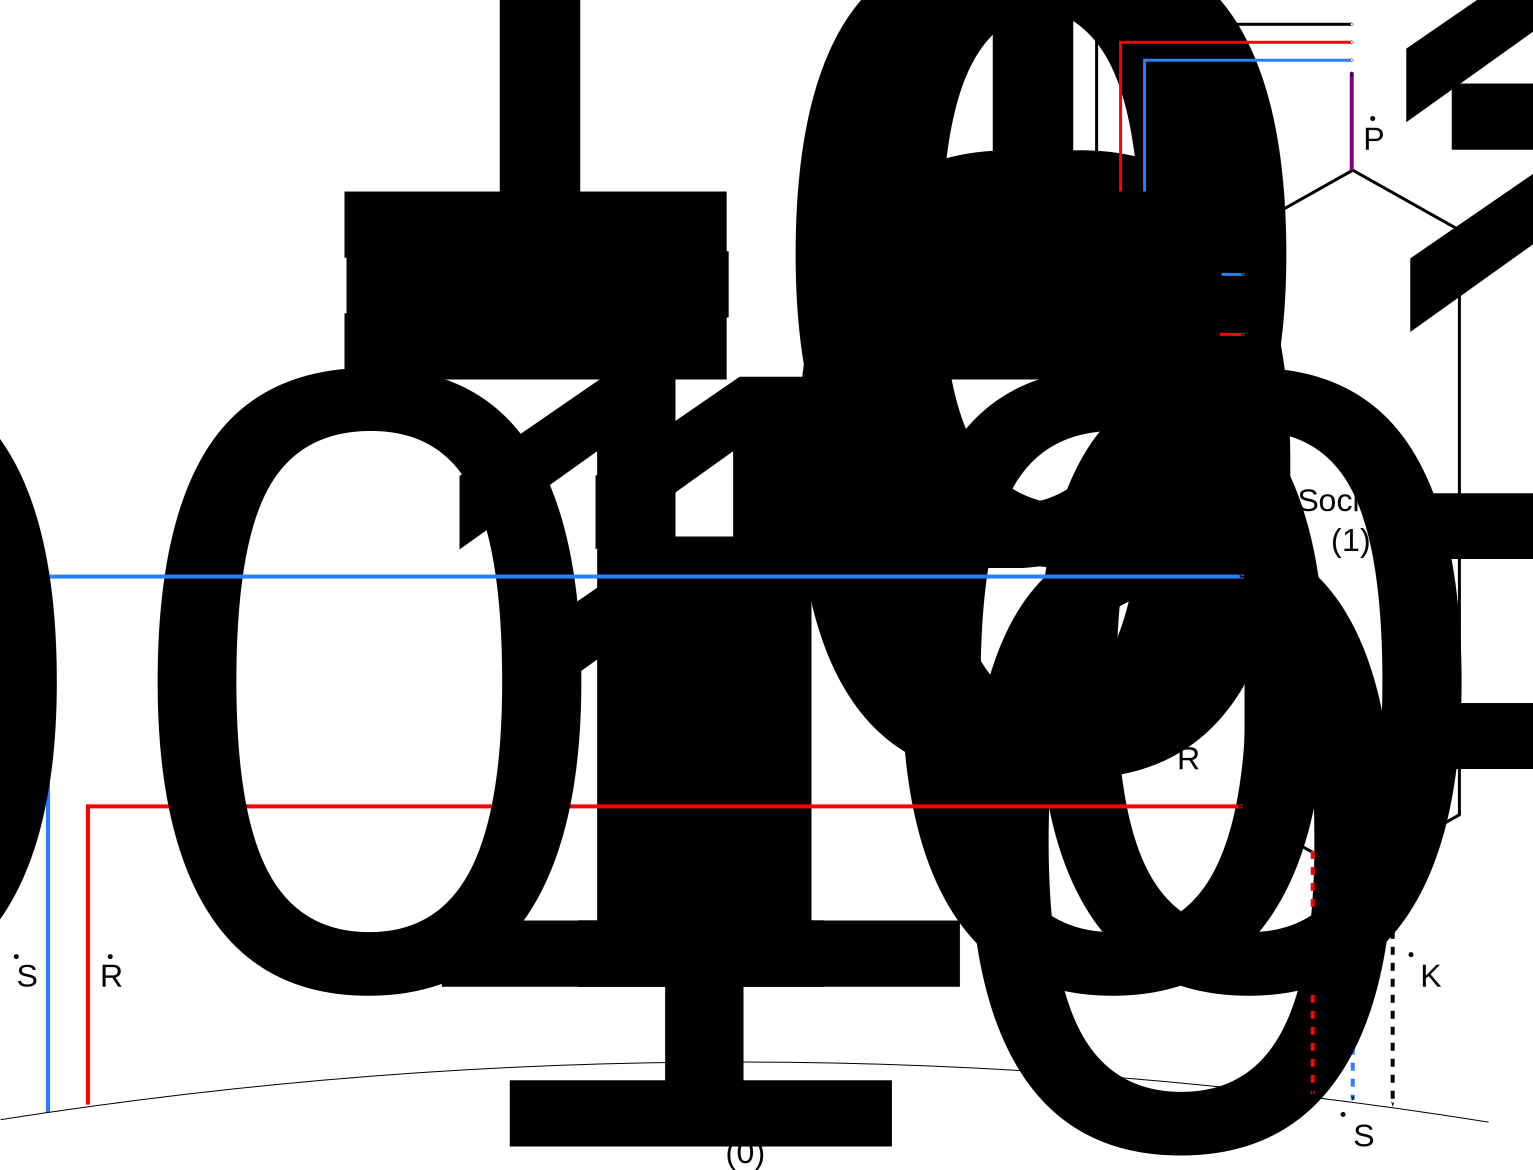
\includegraphics[width=0.8\linewidth]{Part_1/Chapter_Materials/images/1_sector_materials.pdf}
\caption{Flows of materials for a one-sector economy}{Flows of materials for a one-sector economy. 
Resources ($\dot{R}_{01}$) and short-lived materials ($\dot{S}_{01}$) flow into the economy (1) 
from the biosphere (0). Waste resources ($\dot{R}_{10}$) short-lived materials/goods 
($\dot{S}_{10}$) and capital goods ($\dot{K}_{10}$) are returned to the biosphere.}
\label{fig:A_materials}
\end{figure}

Resources, or perhaps more accurately raw materials, ($\dot{R}_{01}$), such as crude oil or iron ore, 
and short-lived materials ($\dot{S}_{01}$), such as oxygen or water that flow \emph{through} economic
processes but are not embodied in the product output, flow into the economy (1) from the biosphere (0). 
These materials are processed within the economy into resource goods, short-lived goods and
capital goods ($\dot{K}$) which are able to be accumulated at some rate $\frac{\mathrm{d}K_{1}}{\mathrm{d}t}$.
Waste resources ($\dot{R}_{10}$) and used short-lived materials/goods ($\dot{S}_{10}$)
are returned to the biosphere without accumulating. Capital goods ($\dot{K}_{10}$) are returned
to the biosphere upon depreciation.

Drawing control volumes around both the biosphere (0) and the economy (1), we can consruct
our material accounting equations, such that:

\begin{align}
\label{eq:A_CV_0_to_1}
	\frac{\mathrm{d}R_0}{\mathrm{d}t}		
	+	\frac{\mathrm{d}S_0}{\mathrm{d}t}
	+	\frac{\mathrm{d}K_0}{\mathrm{d}t}		&	
	=	\dot{R}_{10}		
	+	\dot{S}_{10}	
	+	\dot{K}_{10}											
	-	\dot{R}_{0}											
	-	\dot{S}_{0}								\\
\label{eq:A_CV_0_to_1a}
	\frac{\mathrm{d}R_{1}}{\mathrm{d}t}
	+ \frac{\mathrm{d}S_{1}}{\mathrm{d}t}
	+ \frac{\mathrm{d}K_{1}}{\mathrm{d}t}		&
	= \dot{R}_{01} 
	+ \dot{S}_{01} + \dot{S}_{11}
	- \dot{S}_{1}				
	- \dot{R}_{10}				
	- \dot{S}_{10}				
	- \dot{K}_{10}											
\end{align}

\noindent Remembering that neither resources nor short-lived goods accumulate within economic sectors, tells us that:

\begin{equation}\label{eq:A-dS_1/dt_zero}
	\frac{\mathrm{d}S_1}{\mathrm{d}t}
	= \frac{\mathrm{d}R_1}{\mathrm{d}t}
	= 0.
\end{equation}

\noindent Additionally, we may also say that:

\begin{equation}\label{eq:A_S11}
	\dot{S}_{11} = \dot{S}_{1},
\end{equation}

\noindent such that our material balance equations \ref{eq:A_CV_0_to_1} and \ref{eq:A_CV_0_to_1a} 
become:

%****BRH says, shouldn't this word be
%"accounting" -- not accumulation -- given that is what we
%called it in the sentence introducing eq. 2.4. Or, should we change "accounting" above to accumulation?
%Or, are they synonyms? And, aren't there two of these equations? 2.4 and 2.5? I added a separate
%label for eqn. 2.5**** MIK - Agreed, changed to 'material balance'

\begin{align}\label{eq:A_CV_0_to_1_b}
	\frac{\mathrm{d}R_0}{\mathrm{d}t}		
	+	\frac{\mathrm{d}S_0}{\mathrm{d}t}
	+	\frac{\mathrm{d}K_0}{\mathrm{d}t}		&	
	=	\dot{R}_{10}		
	+	\dot{S}_{10}	
	+	\dot{K}_{10}											
	-	\dot{R}_{0}											
	-	\dot{S}_{0}								\\
	\frac{\mathrm{d}K_{1}}{\mathrm{d}t}		&
	= \dot{R}_{01} 
	+ \dot{S}_{01} 
	- \dot{R}_{10}				
	- \dot{S}_{10}				
	- \dot{K}_{10}											
\end{align}

\noindent Because the only "capital" that accumulates in the biosphere is that which is a waste flow (capital depreciation)
from the economy, e.g. worn-out machines in the scrap yard, we may say that:

\begin{equation} \label{eq:A_K0_balance}
	\frac{\mathrm{d}K_{0}}{\mathrm{d}t}		
	= \dot{K}_{10}
\end{equation}


%%%%%%%%%% Materials: Example B %%%%%%%%%%
\newpage
\section{Example B: two sector economy}
\label{sec:B_materials}
%%%%%%%%%%

In our second example B, we split society into two sectors: production and consumption as depicted in Figure \ref{fig:B_materials}. 

\begin{figure}[h!]
\centering
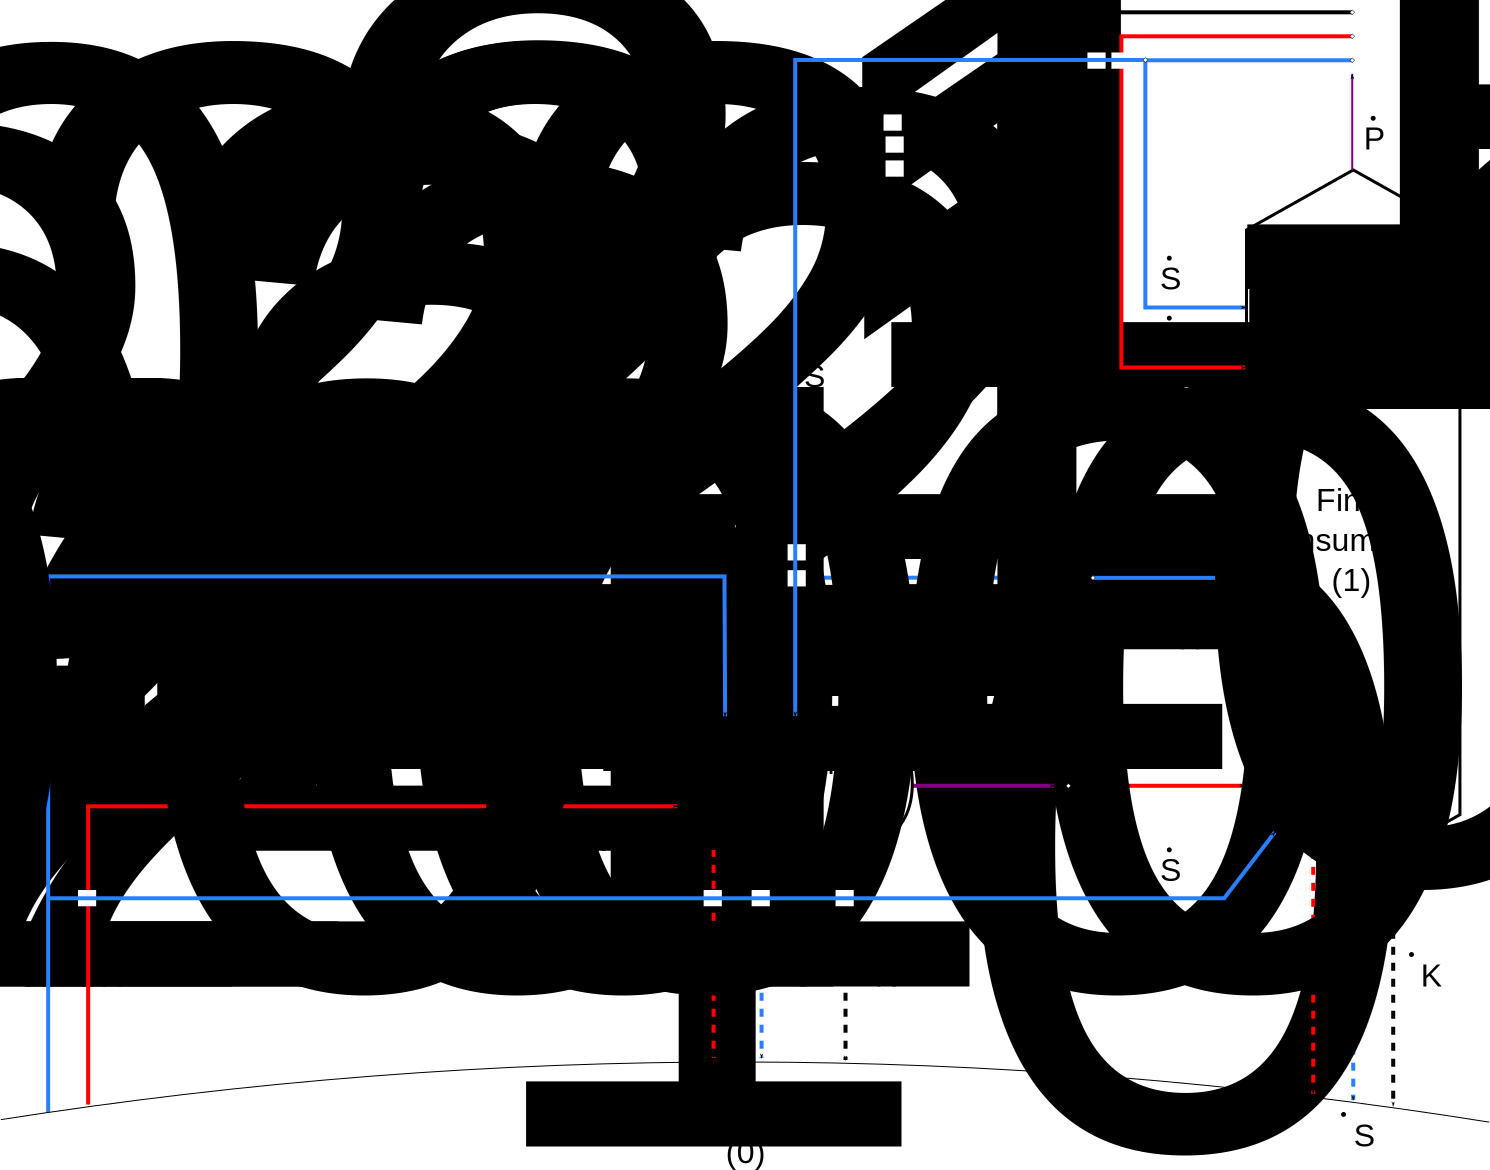
\includegraphics[width=0.8\linewidth]{Part_1/Chapter_Materials/images/2_sector_materials.pdf}
\caption{Flows of materials for a two-sector economy}{Flows of materials for a two-sector economy}
\label{fig:B_materials}
\end{figure}

Sector 2 produces goods and services for consumption in society (1). Again, setting control volumes around the biosphere and our two sectors, our accumulation equations are now written:

\begin{align} \label{eq:B_CV_0_to_2}
	\frac{\mathrm{d}R_{0}}{\mathrm{d}t} 
	+ \frac{\mathrm{d}S_{0}}{\mathrm{d}t}	
	+ \frac{\mathrm{d}K_0}{\mathrm{d}t}		&
	=  \dot{R}_{10} + \dot{R}_{20} 
	+ \dot{S}_{10} + \dot{S}_{20} 
	+ \dot{K}_{10} + \dot{K}_{20} 
	- \dot{R}_{0} 
	- \dot{S}_{0} 							\\
	\frac{\mathrm{d}R_{1}}{\mathrm{d}t} 
	+ \frac{\mathrm{d}S_{1}}{\mathrm{d}t}	
	+ \frac{\mathrm{d}K_{1}}{\mathrm{d}t}	&
	=  \dot{R}_{21} 
	+ \dot{S}_{01} 
	+ \dot{S}_{11} 
	+ \dot{S}_{21}
	+ \dot{K}_{21}
	- \dot{S}_{1} 
	- \dot{R}_{10} 
	- \dot{S}_{10} 
	- \dot{K}_{10},							\\
	\frac{\mathrm{d}R_{2}}{\mathrm{d}t} 
	+ \frac{\mathrm{d}S_{2}}{\mathrm{d}t}
	+ \frac{\mathrm{d}K_{2}}{\mathrm{d}t}	&
	=  \dot{R}_{02} 
	+ \dot{R}_{22} 
	+ \dot{S}_{02} 
	+ \dot{S}_{12} 
	+ \dot{S}_{22} 
	+ \dot{K}_{22}
	- \dot{P}_{2}
	- \dot{R}_{20} 
	- \dot{S}_{20} 
	- \dot{K}_{20},
\end{align}

\begin{equation}
	\dot{R}_{0} = \dot{R}_{02}
\end{equation}

\begin{align}\label{eq:B_S_def}
	\dot{S}_{0} = 
	& \dot{S}_{01} + \dot{S}_{02};
	& \dot{S}_{1} = 
	\dot{S}_{11} + \dot{S}_{12}
\end{align}

Since only capital flows ($\dot{K}$) may be accumulated and are dependent only on flows of capital in and depreciation of capital, we may define capital balance equations:

\begin{equation} \label{eq:B_K1_balance}
	\frac{\mathrm{d}K_{1}}{\mathrm{d}t}
	=  \dot{K}_{12} - \dot{K}_{20},
\end{equation}

[NOT SURE IF THIS IS TRUE IF WE THINK OF $\dot{R}_{12}$ AS FOOD AND $K_{1}$ AS INCLUDING HUMANS... YES, I THINK $\dot{R}_{12}$ CAN BE TURNED INTO  $\dot{K}_{1}$ INTERNALLY, AS THE ACCUMULATION OF (LITERAL) HUMAN CAPITAL, I.E. POPULATION]

\begin{equation} \label{eq:B_K2_balance}
	\frac{\mathrm{d}K_{2}}{\mathrm{d}t}
	=  \dot{K}_{22} - \dot{K}_{20},
\end{equation}

\begin{equation} \label{eq:B_P_def}
	\dot{P}_{2}
	= \dot{R}_{21}
	+ \dot{R}_{22}
	+ \dot{S}_{21}
	+ \dot{S}_{22}
	+ \dot{K}_{21}	 
	+ \dot{K}_{22},
\end{equation}


\noindent Again, remembering that resources and short-lived
goods do not accumulate within sectors of the economy:

\begin{equation}\label{eq:dR_and_dS_zero}
	\frac{\mathrm{d}R_{1}}{\mathrm{d}t}
	= \frac{\mathrm{d}R_{2}}{\mathrm{d}t} 
	= \frac{\mathrm{d}S_{1}}{\mathrm{d}t} 
	= \frac{\mathrm{d}S_{2}}{\mathrm{d}t} 
	= 0,
\end{equation}

\noindent and substituting equations \ref{eq:B_S_def},
\ref{eq:B_K2_balance}  and \ref{eq:B_P_def}, our balance 
equations may now be written:


\begin{align} \label{eq:B_CV_0_to_2_b}
	\frac{\mathrm{d}R_{0}}{\mathrm{d}t} 
	+ \frac{\mathrm{d}S_{0}}{\mathrm{d}t}	
	+ \frac{\mathrm{d}K_0}{\mathrm{d}t}		
	& = \dot{R}_{10} + \dot{R}_{20} 
	+ \dot{S}_{10} + \dot{S}_{20} 
	+ \dot{K}_{10} + \dot{K}_{20} 
	- \dot{R}_{0} 
	- \dot{S}_{0} 							\\
	\frac{\mathrm{d}K_{1}}{\mathrm{d}t}	
	& = \dot{R}_{21} 
	+ \dot{S}_{01} 
	+ \dot{S}_{21}
	+ \dot{K}_{21}
	- \dot{S}_{12} 
	- \dot{R}_{10} 
	- \dot{S}_{10} 
	- \dot{K}_{10},							\\
	\dot{K}_{22} - \dot{K}_{20}	
	& = \dot{R}_{02} 
	+ \dot{S}_{02} 
	+ \dot{S}_{12} 
	- \dot{R}_{21}
	- \dot{S}_{21}
	- \dot{K}_{21}
	- \dot{R}_{20} 
	- \dot{S}_{20} 
	- \dot{K}_{20}							\\
\end{align}





%%%%%%%%%% Materials: Example C %%%%%%%%%%
\newpage
\section{Example C: three sector economy}
\label{sec:C_materials}
%%%%%%%%%%

In example C, we differentiate between two production sectors, one produces energy products and one produces other goods and services.

\begin{figure}[h!]
\centering
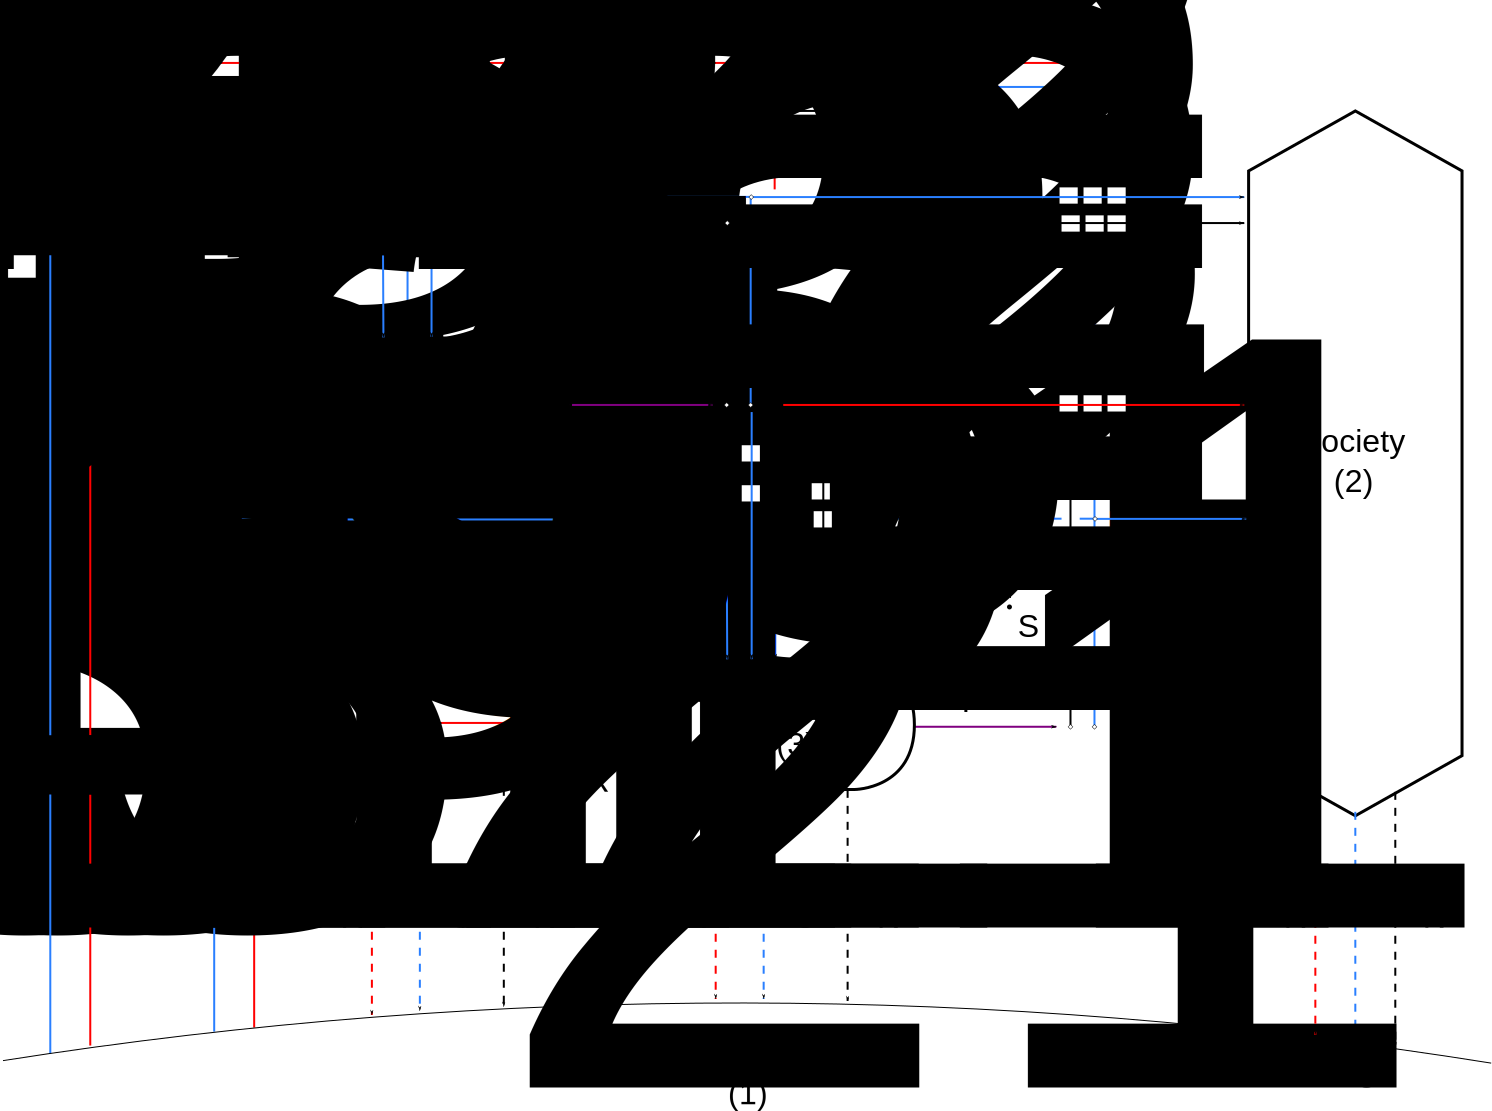
\includegraphics[width=0.8\linewidth]{Part_1/Chapter_Materials/images/3_sector_materials.pdf}
\caption{Flows of materials for a three-sector economy}{Flows of materials for a three-sector economy}
\label{fig:C_materials}
\end{figure}

Accounting for the material flows into and out of the biosphere (sector 0) gives the following equation:

\begin{align} \label{eq:C_CV_0}
	\frac{\mathrm{d}R_{0}}{\mathrm{d}t} 
	+ \frac{\mathrm{d}S_{0}}{\mathrm{d}t}	
	+ \frac{\mathrm{d}K_0}{\mathrm{d}t}		
	& =  \dot{R}_{10} + \dot{R}_{20} + \dot{R}_{30}
	+ \dot{S}_{10} + \dot{S}_{20} + \dot{S}_{30}
	+ \dot{K}_{10} + \dot{K}_{20} + \dot{K}_{30}
	- \dot{R}_{0} 
	- \dot{S}_{0},
\end{align}

\noindent which may be rewritten as:

\begin{align} \label{eq:C_CV_0_b}
	\frac{\mathrm{d}R_{0}}{\mathrm{d}t} 
	+ \frac{\mathrm{d}S_{0}}{\mathrm{d}t}	
	+ \frac{\mathrm{d}K_0}{\mathrm{d}t}		
	& =  \sum_{i = 1}^{3}\dot{R}_{i0}
	+ \sum_{i = 1}^{3}\dot{S}_{i0}
	+ \sum_{i = 1}^{3}\dot{K}_{i0}
	- \dot{R}_{0} 
	- \dot{S}_{0},
\end{align}

Similarly, flows for the other sectors may be written:

\begin{align} \label{eq:C_CV_1_to_3}
	\frac{\mathrm{d}K_{1}}{\mathrm{d}t}		
	& =  \dot{R}_{01} 
	+ \dot{S}_{01}
	+ \sum_{i = 1}^{3}\dot{R}_{i1}
	+ \sum_{i = 1}^{3}\dot{S}_{i1}
	+ \sum_{i = 1}^{3}\dot{K}_{i1}
	- \dot{P}_{1}
	- \dot{R}_{10} 
	- \dot{S}_{10}
	- \dot{K}_{10},										\\
	\frac{\mathrm{d}K_{2}}{\mathrm{d}t}		
	& =  \dot{R}_{02} 
	+ \dot{S}_{02}
	+ \sum_{i = 1}^{3}\dot{R}_{i2}
	+ \sum_{i = 1}^{3}\dot{S}_{i2}
	+ \sum_{i = 1}^{3}\dot{K}_{i2}
	- \dot{P}_{2}
	- \dot{R}_{20} 
	- \dot{S}_{20}
	- \dot{K}_{20},										\\	
	\frac{\mathrm{d}K_{3}}{\mathrm{d}t}		
	& =  \dot{R}_{03} 
	+ \dot{S}_{03}
	+ \sum_{i = 1}^{3}\dot{R}_{i3}
	+ \sum_{i = 1}^{3}\dot{S}_{i3}
	+ \sum_{i = 1}^{3}\dot{K}_{i3}
	- \dot{P}_{3}
	- \dot{R}_{30} 
	- \dot{S}_{30}
	- \dot{K}_{30}.										
\end{align}

These equations may be summarized in one single equation as:

\begin{align} \label{eq:C_CV_1_to_3_b}
	\frac{\mathrm{d}K_{j}}{\mathrm{d}t}		
	& =  \dot{R}_{0j} 
	+ \dot{S}_{0j}
	+ \sum_{i = 1}^{3}\dot{R}_{ij}
	+ \sum_{i = 1}^{3}\dot{S}_{ij}
	+ \sum_{i = 1}^{3}\dot{K}_{ij}
	- \dot{P}_{j}
	- \dot{R}_{j0} 
	- \dot{S}_{j0}
	- \dot{K}_{j0};
	& j \in \left[1,3\right].
\end{align}

Again, we can say that:

\begin{align} \label{eq:C_CV_K_balance}
	\frac{\mathrm{d}K_{j}}{\mathrm{d}t}		
	& =  \sum_{i = 1}^{3}\dot{K}_{ij}
	- \dot{K}_{j0};
\end{align}

\noindent hence we may say that:

\begin{align} \label{eq:C_CV_1_to_3_b}
	\dot{R}_{0j} 
	+ \dot{S}_{0j}
	+ \sum_{i = 1}^{3}\dot{R}_{ij}
	+ \sum_{i = 1}^{3}\dot{S}_{ij}
	& = \dot{P}_{j}
	- \dot{R}_{j0} 
	- \dot{S}_{j0}.
\end{align}



\begin{figure}[h!]
\centering
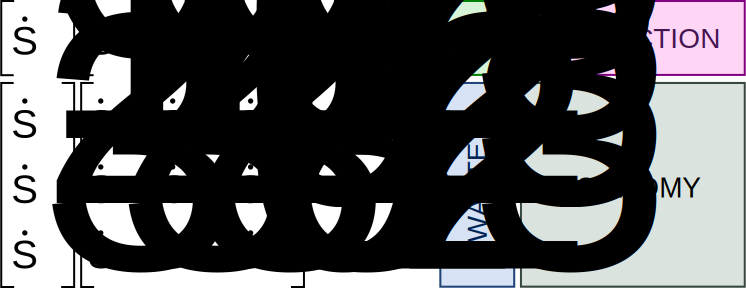
\includegraphics[width=0.8\linewidth]{Part_1/Chapter_Materials/images/Matrix.pdf}
\caption{The matrix of biosphere-economy flows}{The matrix of biosphere-economy flows}
\label{fig:C_mat_matrix}
\end{figure}

%%%%%%%%%% Materials: Auto industry example %%%%%%%%%%
\section{Materials in the auto industry}
\label{sec:materials_auto}
%%%%%%%%%%

%%%%%%%%%% Materials: Summary %%%%%%%%%%
\section{Summary}
\label{sec:materials_summary}
%%%%%%%%%%

\bibliography{../../EROI_review_v2}
\bibliographystyle{unsrt}


% Always give a unique label
% and use \ref{<label>} for cross-references
% and \cite{<label>} for bibliographic references
% use \sectionmark{}
% to alter or adjust the section heading in the running head
%% Instead of simply listing headings of different levels we recommend to let every heading be followed by at least a short passage of text. Furtheron please use the \LaTeX\ automatism for all your cross-references and citations.

%% Please note that the first line of text that follows a heading is not indented, whereas the first lines of all sequent paragraphs are.

%% Use the standard \verb|equation| environment to typeset your equations, e.g.
%
%% \begin{equation}
%% a \times b = c\;,
%% \end{equation}
%
%% however, for multiline equations we recommend to use the \verb|eqnarray|
%% environment\footnote{In physics texts please activate the class option \texttt{vecphys} to depict your vectors in \textbf{\itshape boldface-italic} type - as is customary for a wide range of physical jects.}.
%%\begin{eqnarray}
%%a \times b = c \nonumber\\
%% \vec{a} \cdot \vec{b}=\vec{c}
%% \label{eq:01}
%%\end{eqnarray}

%% \section{section Heading}
%% \label{sec:2}
%% Instead of simply listing headings of different levels we recommend to let every heading be followed by at least a short passage of text. Furtheron please use the \LaTeX\ automatism for all your cross-references\index{cross-references} and citations\index{citations} as has already been described in Sect.~\ref{sec:2}.

%% \begin{quotation}
%% Please do not use quotation marks when quoting texts! Simply use the \verb|quotation| environment -- it will automatically render Springer's preferred layout.
%% \end{quotation}


%% \section{section Heading}
%% Instead of simply listing headings of different levels we recommend to let every heading be followed by at least a short passage of text. Furtheron please use the \LaTeX\ automatism for all your cross-references and citations as has already been described in Sect.~\ref{sec:2}, see also Fig.~\ref{fig:1}\footnote{If you copy text passages, figures, or tables from other works, you must obtain \textit{permission} from the copyright holder (usually the original publisher). Please enclose the signed permission with the manucript. The sources\index{permission to print} must be acknowledged either in the captions, as footnotes or in a separate section of the book.}

%% Please note that the first line of text that follows a heading is not indented, whereas the first lines of all sequent paragraphs are.

% For figures use
%
%% \begin{figure}[b]
%% \sidecaption
% Use the relevant command for your figure-insertion program
% to insert the figure file.
% For example, with the option graphics use
%% \includegraphics[scale=.65]{figure}
%
% If not, use
%\picplace{5cm}{2cm} % Give the correct figure height and width in cm
%
%% \caption{If the width of the figure is less than 7.8 cm use the \texttt{sidecapion} command to flush the caption on the left side of the page. If the figure is positioned at the top of the page, align the sidecaption with the top of the figure -- to achieve this you simply need to use the optional argument \texttt{[t]} with the \texttt{sidecaption} command}
%% \label{fig:1}       % Give a unique label
%% \end{figure}


%% \paragraph{Paragraph Heading} %
%% Instead of simply listing headings of different levels we recommend to let every heading be followed by at least a short passage of text. Furtheron please use the \LaTeX\ automatism for all your cross-references and citations as has already been described in Sect.~\ref{sec:2}.

%% Please note that the first line of text that follows a heading is not indented, whereas the first lines of all sequent paragraphs are.

%% For typesetting numbered lists we recommend to use the \verb|enumerate| environment -- it will automatically render Springer's preferred layout.

%% \begin{enumerate}
%% \item{Livelihood and survival mobility are oftentimes coutcomes of uneven socioeconomic development.}
%% \begin{enumerate}
%% \item{Livelihood and survival mobility are oftentimes coutcomes of uneven socioeconomic development.}
%% \item{Livelihood and survival mobility are oftentimes coutcomes of uneven socioeconomic development.}
%% \end{enumerate}
%% \item{Livelihood and survival mobility are oftentimes coutcomes of uneven socioeconomic development.}
%% \end{enumerate}


%% \paragraph{paragraph Heading} In order to avoid simply listing headings of different levels we recommend to let every heading be followed by at least a short passage of text. Use the \LaTeX\ automatism for all your cross-references and citations as has already been described in Sect.~\ref{sec:2}, see also Fig.~\ref{fig:2}.

%% Please note that the first line of text that follows a heading is not indented, whereas the first lines of all sequent paragraphs are.

%% For unnumbered list we recommend to use the \verb|itemize| environment -- it will automatically render Springer's preferred layout.

%% \begin{itemize}
%% \item{Livelihood and survival mobility are oftentimes coutcomes of uneven socioeconomic development, cf. Table~\ref{tab:1}.}
%% \begin{itemize}
%% \item{Livelihood and survival mobility are oftentimes coutcomes of uneven socioeconomic development.}
%% \item{Livelihood and survival mobility are oftentimes coutcomes of uneven socioeconomic development.}
%% \end{itemize}
%% \item{Livelihood and survival mobility are oftentimes coutcomes of uneven socioeconomic development.}
%% \end{itemize}

%% \begin{figure}[t]
%% \sidecaption[t]
% Use the relevant command for your figure-insertion program
% to insert the figure file.
% For example, with the option graphics use
%% \includegraphics[scale=.65]{figure}
%
% If not, use
%\picplace{5cm}{2cm} % Give the correct figure height and width in cm
%
%% \caption{Please write your figure caption here}
%% \label{fig:2}       % Give a unique label
%% \end{figure}

%% \runinhead{Run-in Heading Boldface Version} Use the \LaTeX\ automatism for all your cross-references and citations as has already been described in Sect.~\ref{sec:2}.

%% \runinhead{Run-in Heading Italic Version} Use the \LaTeX\ automatism for all your cross-refer\-ences and citations as has already been described in Sect.~\ref{sec:2}\index{paragraph}.
% Use the \index{} command to code your index words
%
% For tables use
%
%% \begin{table}
%% \caption{Please write your table caption here}
%% \label{tab:1}       % Give a unique label
%
% For LaTeX tables use
%
%% \begin{tabular}{p{2cm}p{2.4cm}p{2cm}p{4.9cm}}
%% \hline\noalign{\smallskip}
%% Classes & class & Length & Action Mechanism  \\
%% \noalign{\smallskip}\svhline\noalign{\smallskip}
%% Translation & mRNA$^a$  & 22 (19--25) & Translation repression, mRNA cleavage\\
%% Translation & mRNA cleavage & 21 & mRNA cleavage\\
%% Translation & mRNA  & 21--22 & mRNA cleavage\\
%%Translation & mRNA  & 24--26 & Histone and DNA Modification\\
%%\noalign{\smallskip}\hline\noalign{\smallskip}
%%\end{tabular}
%%$^a$ Table foot note (with superscript)
%%\end{table}
%
%% \section{Section Heading}
%%\label{sec:3}
% Always give a unique label
% and use \ref{<label>} for cross-references
% and \cite{<label>} for bibliographic references
% use \sectionmark{}
% to alter or adjust the section heading in the running head
%% Instead of simply listing headings of different levels we recommend to let every heading be followed by at least a short passage of text. Furtheron please use the \LaTeX\ automatism for all your cross-references and citations as has already been described in Sect.~\ref{sec:2}.

%% Please note that the first line of text that follows a heading is not indented, whereas the first lines of all sequent paragraphs are.

%%If you want to list definitions or the like we recommend to use the Springer-enhanced \verb|description| environment -- it will automatically render Springer's preferred layout.

%%\begin{description}[Type 1]
%%\item[Type 1]{That addresses central themes pertainng to migration, health, and disease. In Sect.~\ref{sec:1}, Wilson discusses the role of human migration in infectious disease distributions and patterns.}
%%\item[Type 2]{That addresses central themes pertainng to migration, health, and disease. In Sect.~\ref{sec:2}, Wilson discusses the role of human migration in infectious disease distributions and patterns.}
%%\end{description}

%%\section{section Heading} %
%% In order to avoid simply listing headings of different levels we recommend to let every heading be followed by at least a short passage of text. Use the \LaTeX\ automatism for all your cross-references and citations citations as has already been described in Sect.~\ref{sec:2}.

%% Please note that the first line of text that follows a heading is not indented, whereas the first lines of all sequent paragraphs are.

%% \begin{svgraybox}
%% If you want to emphasize complete paragraphs of texts we recommend to use the newly defined Springer class option \verb|graybox| and the newly defined environment \verb|svgraybox|. This will produce a 15 percent screened box 'behind' your text.

%% If you want to emphasize complete paragraphs of texts we recommend to use the newly defined Springer class option and environment \verb|svgraybox|. This will produce a 15 percent screened box 'behind' your text.
%% \end{svgraybox}


%% \section{section Heading}
%%Instead of simply listing headings of different levels we recommend to let every heading be followed by at least a short passage of text. Furtheron please use the \LaTeX\ automatism for all your cross-references and citations as has already been described in Sect.~\ref{sec:2}.

%% Please note that the first line of text that follows a heading is not indented, whereas the first lines of all sequent paragraphs are.

%% \begin{theorem}
%% Theorem text goes here.
%% \end{theorem}
%
% or
%
%% \begin{definition}
%% Definition text goes here.
%% \end{definition}

%% \begin{proof}
%\smartqed
%% Proof text goes here.
%% \qed
%% \end{proof}

%%\paragraph{Paragraph Heading} %
%% Instead of simply listing headings of different levels we recommend to let every heading be followed by at least a short passage of text. Furtheron please use the \LaTeX\ automatism for all your cross-references and citations as has already been described in Sect.~\ref{sec:2}.

%% Note that the first line of text that follows a heading is not indented, whereas the first lines of all subsequent paragraphs are.
%
% For built-in environments use
%
%%\begin{theorem}
%%Theorem text goes here.
%%\end{theorem}
%
%%\begin{definition}
%%Definition text goes here.
%%\end{definition}
%
%%\begin{proof}
%%\smartqed
%% Proof text goes here.
%%\qed
%%\end{proof}
%
%% \begin{acknowledgement}
%% If you want to include acknowledgments of assistance and the like at the end of an individual chapter please use the \verb|acknowledgement| environment -- it will automatically render Springer's preferred layout.
%% \end{acknowledgement}
%
%% \section*{Appendix}
%% \addcontentsline{toc}{section}{Appendix}
%
%% When placed at the end of a chapter or contribution (as opposed to at the end of the book), the numbering of tables, figures, and equations in the appendix section continues on from that in the main text. Hence please \textit{do not} use the \verb|appendix| command when writing an appendix at the end of your chapter or contribution. If there is only one the appendix is designated ``Appendix'', or ``Appendix 1'', or ``Appendix 2'', etc. if there is more than one.

%% \begin{equation}
%% a \times b = c
%% \end{equation}
% Problems or Exercises should be sorted chapterwise
%% \section*{Problems}
%% \addcontentsline{toc}{section}{Problems}
%
% Use the following environment.
% Don't forget to label each problem;
% the label is needed for the solutions' environment
%% \begin{prob}
%% \label{prob1}
%% A given problem or Excercise is described here. The
%% problem is described here. The problem is described here.
%% \end{prob}

%% \begin{prob}
%% \label{prob2}
%% \textbf{Problem Heading}\\
%% (a) The first part of the problem is described here.\\
%% (b) The second part of the problem is described here.
%% \end{prob}




%!TEX root = ../../Heun_Dale_Haney_A_dynamic_approach_to_input_output_modeling.tex
%%%%%%%%%%%%%%%%%%%%% chapter.tex %%%%%%%%%%%%%%%%%%%%%%%%%%%%%%%%%
%
% sample chapter
%
% Use this file as a template for your own input.
%
%%%%%%%%%%%%%%%%%%%%%%%% Springer-Verlag %%%%%%%%%%%%%%%%%%%%%%%%%%
%\motto{Use the template \emph{chapter.tex} to style the various elements of your chapter content.}
\motto{Living organisms need to be open 
to a constant flow of resources~(energy and matter) 
to stay alive; \\
human organizations need to be open 
to a flow of mental resources~(information and ideas), 
as well as to the flows of energy and materials 
that are part of the production \\
of goods or services.~\emph{\cite[p.117]{Capra2004}}

\hfill---\emph{Fritjof Capra}}

%%%%%%%%%%%%%%%%%%%%%%%%%%%%%%%%%%%%%%%%%
%%%%%%%%%% Direct Energy Flows %%%%%%%%%%
%%%%%%%%%%%%%%%%%%%%%%%%%%%%%%%%%%%%%%%%%
\chapter{Direct energy flows}
% Always give a unique label
\label{chap:direct_energy} 
% use \chaptermark{} to alter or adjust the chapter heading in the running head
\chaptermark{Direct energy}
%%%%%%%%%%%%%%%%%%%%%%%%%%%%%%%%%%%%%%%%%
%%%%%%%%%%%%%%%%%%%%%%%%%%%%%%%%%%%%%%%%%
%%%%%%%%%%%%%%%%%%%%%%%%%%%%%%%%%%%%%%%%%

%% \abstract{Each chapter should be preceded by an abstract (10--15 lines long) that summarizes the content. The abstract will appear \textit{online} at \url{www.SpringerLink.com} and be available with unrestricted access. This allows unregistered users to read the abstract as a teaser for the complete chapter. As a general rule the abstracts will not appear in the printed version of your book unless it is the style of your particular book or that of the series to which your book belongs.\newline\indent
%% Please use the 'starred' version of the new Springer \texttt{abstract} command for typesetting the text of the online abstracts (cf. source file of this chapter template \texttt{abstract}) and include them with the source files of your manuscript. Use the plain \texttt{abstract} command if the abstract is also to appear in the printed version of the book.}

%% Use the template \emph{chapter.tex} together with the Springer document class SVMono (monograph-type books) or SVMult (edited books) to style the various elements of your chapter content in the Springer layout.

\abstract*{In this chapter, we develop equations, 
assisted by the First Law of Thermodynamics,
that describe the flow of 
direct energy through economies.
The equations are applied to
example economies with increasing levels of disaggregation. 
Finally, the energy flows for our running example, the US auto industry,
are discussed.}

In Chapter~\ref{chap:intro}, we formulated a model of economies
consisting of producers and consumers who exchange
goods and services and factors of production 
while extracting resources and disposing of wastes. 
In Chapter~\ref{chap:materials}, we established the material basis of economies: 
economies are analogous to organisms with metabolisms that processes
raw resources for the benefit of producers and consumers 
while generating unavoidable wastes.
In this chapter, we describe and analyze the 
direct energy
that is associated with material flows
through an economy.

All forms of energy provide the potential to do mechanical work.\footnote{The 
quantification of the mechanical work potential of energy is \emph{exergy}.
When energy is ``consumed'' by an economy, exergy (work potential) is destroyed.
These topics are discussed in greater detail in Section~\ref{sec:material_quality}.}
Energy (as mechanical work) 
is an essential aspect of the metabolic economy;
with it, materials are refined, shaped, and assembled
into useful intermediate and final products; 
food is made available to people in society; 
jobs are made easier for workers;
human ingenuity is multiplied;
and complex systems and civilizations are possible.
In the absence of high rates of energy availablity at low cost,
life becomes much more difficult, even impossible, for many people.

The analogy for this chapter is this: 
energy is to thermodynamics as money is to financial accounting.
Or, energy is the \emph{currency of thermodynamics}.
Just as an accountant understands a firm by watching how and where
currency flows through it, so we can understand an economy by watching
how and where energy flows through it.
Accounting for energy flows through an economy
is essential for developing a dynamic picture 
of its metabolism.

The purpose of this chapter is to develop 
a framework for accounting energy flows within economies.
With an energy model in hand, we will be positioned 
to assess the rate at which
consumed direct energy becomes embodied within the products and 
services that an economy provides
(Chapter~\ref{chap:embodied_energy}).


%%%%%%%%%% Energy: Methodology %%%%%%%%%%
\section{Methodology}
\label{sec:energy_methodology}
%%%%%%%%%%

We begin by noting that direct energy travels 
with material through an economy.
``Direct'' energy refers to forms of energy accounted by the 
First Law of Thermodynamics,
including chemical potential energy, 
nuclear potential energy, 
gravitational potential energy,
thermal energy, 
and kinetic energy.
We use the term ``direct'' energy distinct from ``embodied'' energy, 
which will be discussed in Chapter~\ref{chap:embodied_energy}.
Examples of direct energy flows include 
the chemical potential energy of coal inflows to an energy sector, 
the thermal energy of process steam into a textile plant, and
the thermal energy of CO$_2$ automobile exhaust.
Each of these example flows is an example of a ``transfer in''
or a ``transfer out,'' in the language % chktex 38
of Section~\ref{sec:accounting_in_everyday_life}.
In each case, the material (coal, steam, and CO$_2$) 
carries direct energy with it.
Figure~\ref{fig:PERKS_energy_content} shows a corresponding 
direct energy flow for each material flow of Figure~\ref{fig:PERKS_materials}.

\begin{figure}[!ht]
\centering\
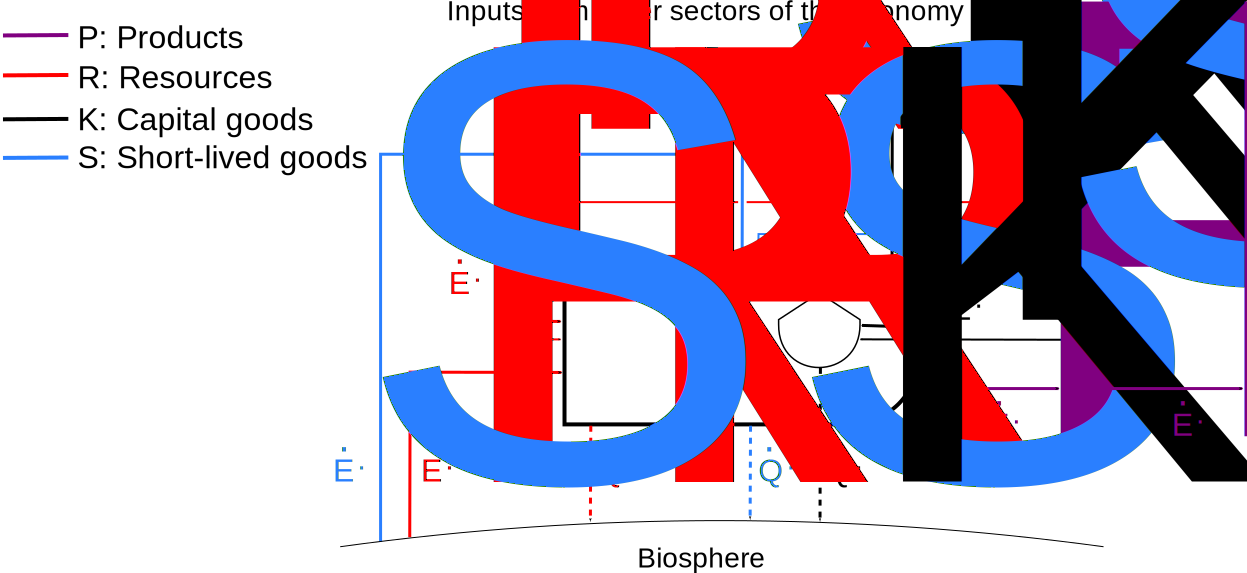
\includegraphics[width=0.8\linewidth]{Part_1/Chapter_Energy/images/PERKS_basic_unit_energy_content.pdf}
\caption[Energy content of material flows for a single sector]{Energy content ($\dot{E}$) of material flows 
($\dot{R}$, $\dot{S}$, and $\dot{K}$) 
from Figure~\ref{fig:PERKS_materials}.}
\label{fig:PERKS_energy_content}
\end{figure}

For any boundary (around, say, a machine, a plant,
a sector of the economy, or the entire economy itself), 
the First Law of Thermodynamics says that 
the accumulation rate 
of direct energy within the 
boundary $\left( \frac{\mathrm{d}E}{\mathrm{d}t} \right)$
is equal to the sum of the incoming and outgoing direct energy transfer 
rates ($\dot{E}$)
less outflowing energy carried by wastes 
($\dot{Q}_{out}$). 
Energy is conserved: it be neither created nor destroyed.

\begin{equation} \label{eq:First_Law_with_accumulation}
	\frac{\mathrm{d}E}{\mathrm{d}t} = \sum \dot{E} - \sum \dot{Q}_{out}
\end{equation}

When there is no accumulation of direct energy within the boundary
$\left( \frac{\mathrm{d}E}{\mathrm{d}t} = 0 \right)$, the sum of all 
signed direct energy flow rates ($\dot{E}$) 
and waste heats ($\dot{Q}_{out}$) will be zero.

\begin{equation} \label{eq:First_Law_no_accumulation}
	0 = \sum \dot{E} - \sum \dot{Q}_{out}
\end{equation}

It is important to note that the direct energy associated with some material flows can
be so small as to be negligible compared to other direct energy flows in the economy.
For example, there is a small amount of chemical energy in steel that could be
released upon combustion. 
However, the direct energy associated flows of steel within the economy
is almost negligible. (The \emph{embodied} energy of the steel is most certainly
\emph{not} negligible, as will be discussed in Chapter~\ref{chap:embodied_energy}.)
On the other hand, the direct energy flow rates for 
fossil fuels
(coal, oil, and natural gas)
are typically orders of magnitude larger than any other 
material flows due to large chemical potential energy content.

To simplify the direct energy analysis, 
we can aggregate the direct energy flows of Figure~\ref{fig:PERKS_energy_content}
into single arrows when appropriate. 
For example, the direct energy inputs from other sectors of the economy
(labeled as $\dot{E}_{\dot{R}}$, $\dot{E}_{\dot{S}}$, and $\dot{E}_{\dot{K}}$ 
at the top of Figure~\ref{fig:PERKS_energy_content}) can be summed to $\dot{E}$ 
(in Figure~\ref{fig:PERKS_energy}) such that

\begin{equation} \label{eq:direct_energy_aggregation}
	\dot{E} 
	= \dot{E}_{\dot{R}} 
	+ \dot{E}_{\dot{S}} 
	+ \dot{E}_{\dot{K}}.
\end{equation}

\begin{figure}[!ht]
\centering
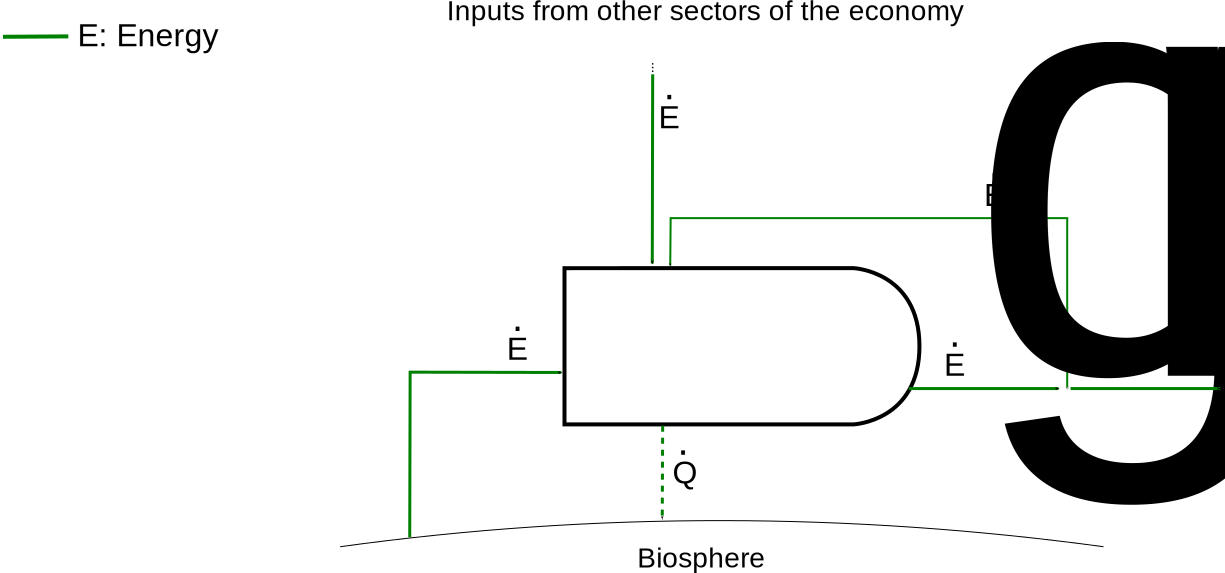
\includegraphics[width=0.8\linewidth]{Part_1/Chapter_Energy/images/PERKS_basic_unit_energy.pdf}
\caption[Aggregated direct energy flows for a single sector]{Aggregated direct energy flows ($\dot{E}$) around 
the producer of Figure~\ref{fig:PERKS_energy_content}.}
\label{fig:PERKS_energy}
\end{figure}


%%%%%%%%%% Energy: Example A %%%%%%%%%%
\section{Example A: single-sector economy} % chktex 13
\label{sec:A_energy}
%%%%%%%%%%

Aggregated direct energy flows are now applied to Example A, 
the single-sector economy shown in Figure~\ref{fig:A_materials}.
By summing the direct energy flows associated with
each material flow of Figure~\ref{fig:A_materials}, we obtain
a simplified picture of direct energy flows in the economy,
as shown in Figure~\ref{fig:A_energy}.

\begin{figure}[!ht]
\centering
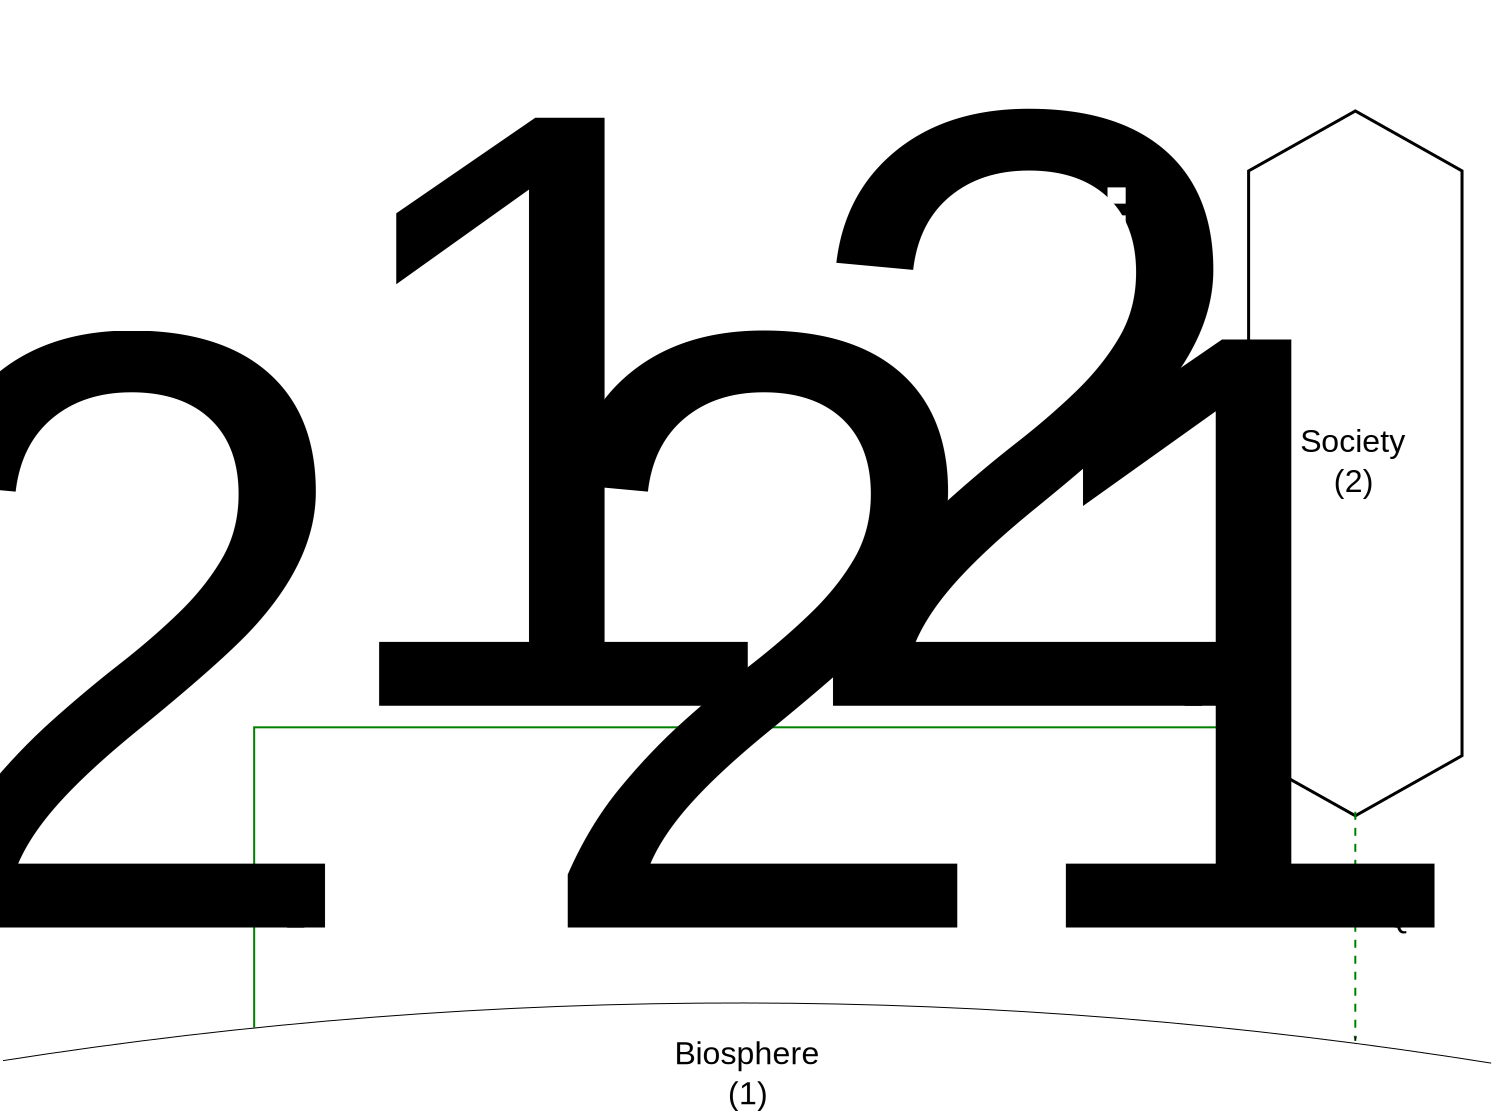
\includegraphics[width=0.8\linewidth]{Part_1/Chapter_Energy/images/1_sector_direct_energy.pdf}
\caption[Direct energy flows a one-sector economy]{Direct energy flows ($\dot{E}$) a one-sector economy.}
\label{fig:A_energy}
\end{figure}

We distinguish useful direct energy inputs to a sector of the economy
($\dot{E}_{01}$ in Figure~\ref{fig:A_energy}) from wasteful direct energy flows 
($\dot{Q}_{10}$ in Figure~\ref{fig:A_energy}), 
because $\dot{Q}$ typically denotes thermal energy, 
and most waste energy is in the form of thermal
energy, i.e., waste heat. In Figure~\ref{fig:A_energy}, direct energy input to the 
economy ($\dot{E}_{01}$) is shown as being extracted from the biosphere, because
the vast majority of direct energy today is derived from fossil fuels.
Waste heat from the economy ($\dot{Q}_{10}$) is shown as returning 
to the biosphere.

As discussed in Section~\ref{sec:energy_methodology}, 
both direct energy ($\dot{E}$), and waste heat ($\dot{Q}$) 
are accounted by the First Law of Thermodynamics. 
Accounting for possible accumulation of direct energy, 
the First Law of Thermodynamics for Example~A indicates that

\begin{equation} \label{eq:dE_0/dt_single_sector}
	\frac{\mathrm{d}E_0}{\mathrm{d}t} 
	= \dot{Q}_{10} 
	- \dot{E}_{01}
\end{equation}

\noindent and

\begin{equation} \label{eq:dE_1/dt_single_sector}
	\frac{\mathrm{d}E_{1}}{\mathrm{d}t} 
	= \dot{E}_{01} 
	+ \dot{E}_{11}
	- \dot{E}_{1}
	- \dot{Q}_{10}.
\end{equation}

Note that $\dot{E}_{1}$ is the gross direct energy production rate
of society. 
For example, firms extract crude oil (a component of $\dot{E}_{01}$) 
and refine it into petroleum products (a component of $\dot{E}_{1}$)
that are consumed by society.
The direct energy consumption of extraction and refining firms 
is a component of $\dot{E}_{11}$.

Aside from, for example, the US 
Strategic Petroleum Reserve, 
we are not stockpiling oil and coal at any meaningful rate, 
i.e.\ we consume fossil fuels at a rate equal to their extraction rate. 
Thus, the world is not accumulating direct energy 
in the economy.\footnote{A counter-example could be made 
for nuclear fuels where ``spent'' fuel represents a large exergetic stockpile. 
However, this reserve is not (presently) economically useful.} 
(The world \emph{is}, however, 
accumulating \emph{embodied} energy
in the economy as we shall see 
in Chapter~\ref{chap:embodied_energy}.) 
Thus, the accumulation rates for direct energy 
$\left( \frac{\mathrm{d}E}{\mathrm{d}t} \right)$ in the above equations 
could be set to zero as follows:

\begin{equation} \label{eq:biosphere_direct_energy_steady_state}
	0 
	= \dot{Q}_{10} 
	- \dot{E}_{01}
\end{equation}

\noindent and

\begin{equation} \label{eq:single_sector_direct_energy_steady_state}
	0 
	= \dot{E}_{01} 
	+ \dot{E}_{11}
	- \dot{E}_{1} 
	- \dot{Q}_{10}.
\end{equation}

\noindent{}However, we shall see later (in Chapter~\ref{chap:direct_energy}) 
that keeping direct energy accumulation terms
$\left( \frac{\mathrm{d}E}{\mathrm{d}t} \right)$ 
provides an advantage when deriving embodied energy accounting equations.


%%%%%%%%%% Energy: Example B %%%%%%%%%%
\section{Example B: two-sector economy} % chktex 13
\label{sec:B_energy}
%%%%%%%%%%

For Example~B, we split a Production sector (2) from 
society (1). Figure~\ref{fig:B_energy} shows aggregated
direct energy flows associated with the material flows of Figure~\ref{fig:B_materials}.

\begin{figure}[!ht]
\centering
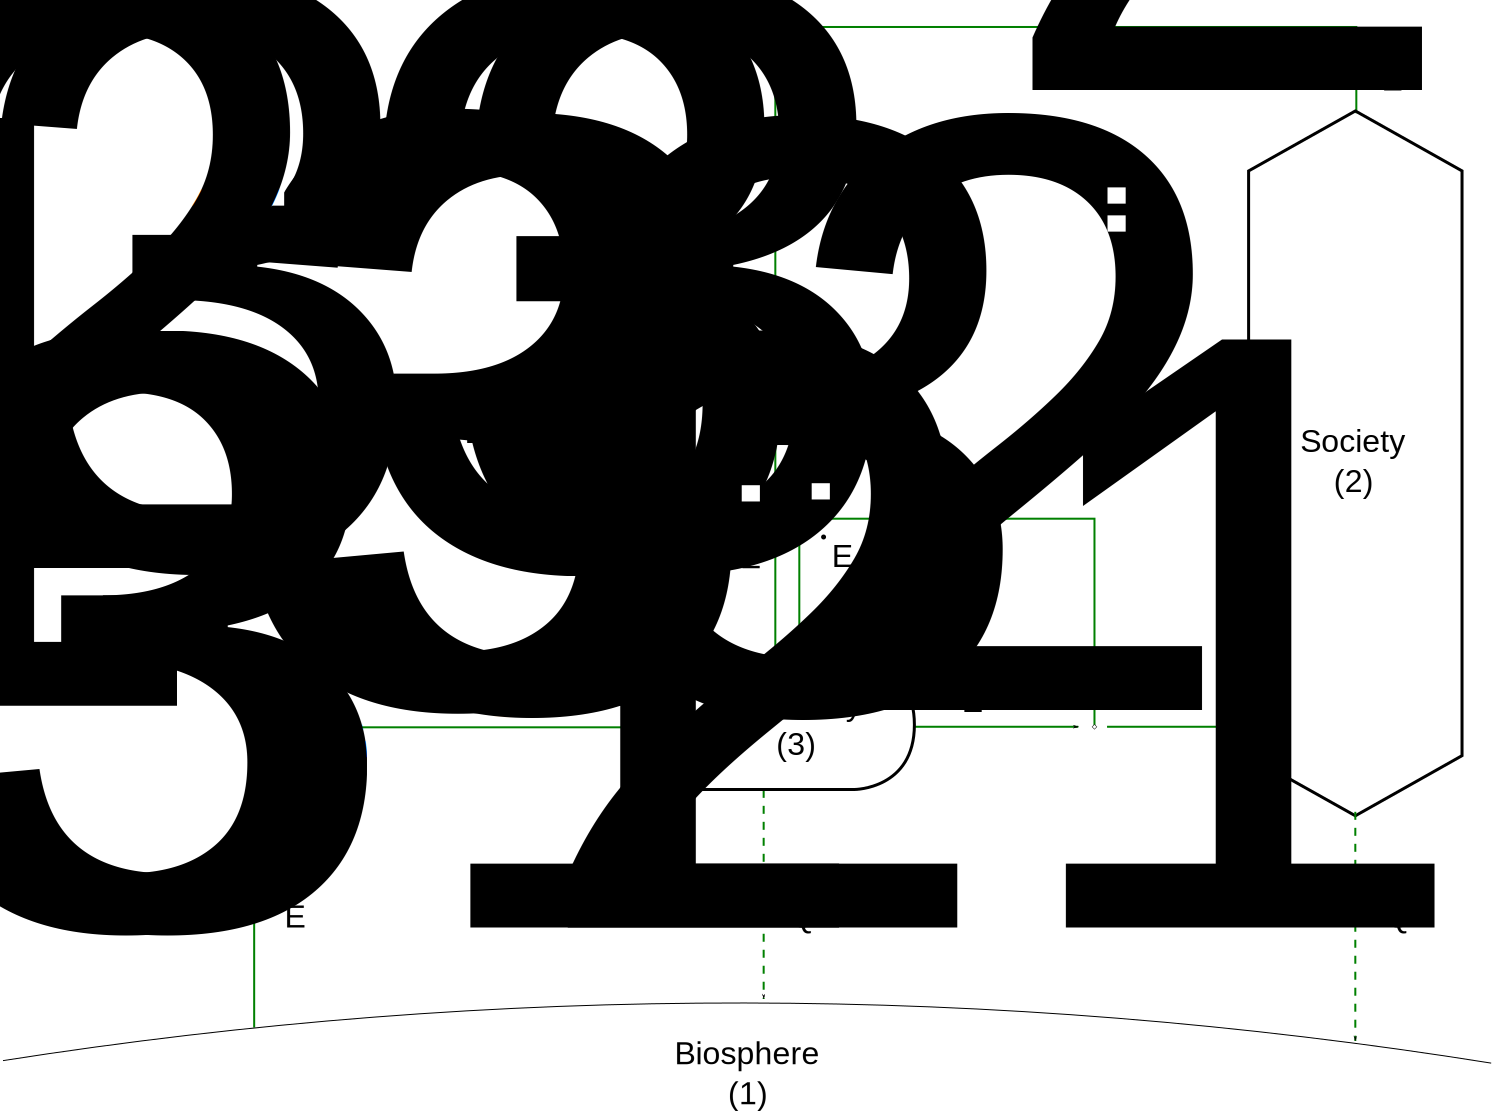
\includegraphics[width=0.8\linewidth]{Part_1/Chapter_Energy/images/2_sector_direct_energy.pdf}
\caption[Direct energy flows for a two-sector economy]{Direct energy flows ($\dot{E}$) for a two-sector economy.}
\label{fig:B_energy}
\end{figure}

The First Law of Thermodynamics
requires that both 
direct energy and 
waste heat
be conserved around each 
entity (1 and 2) as well as around the biosphere (0).

\noindent{}First Law energy accounting around the biosphere (0) and society (1) gives

\begin{equation} \label{eq:CV_E_dot_0}
	\frac{\mathrm{d}E_{0}}{\mathrm{d}t} 	 
	= \dot{Q}_{10} 
	+ \dot{Q}_{20} 
	- \dot{E}_{02},
\end{equation}

\noindent and 

\begin{equation} \label{eq:CV_E_dot_1}
	\frac{\mathrm{d}E_{1}}{\mathrm{d}t} 	 
	= \dot{E}_{11} 
	+ \dot{E}_{21}
	- \dot{E}_{1}
	- \dot{Q}_{10}.
\end{equation}

Note that $\dot{E}_{12}$ represents useful work that people
and draught animals contribute to Production (2). 
Ayres and Warr~\cite{Ayres:2003ec,Warr:2012cg} call this ``muscle work.'' 
$\dot{E}_{11}$ represents the muscle work required for consumption. 
Direct energy (electricity, oil, natural gas, etc.) 
required for consumption by final demand 
is included in $\dot{E}_{21}$.

The First Law around Production (2), 
including the accumulation rate of direct energy in the sector 
$\left(\frac{\mathrm{d}E_{2}}{\mathrm{d}t}\right)$, yields

\begin{equation} \label{eq:CV_E_dot_2}
	\frac{\mathrm{d}E_{2}}{\mathrm{d}t} 
	= \dot{E}_{02} 
	+ \dot{E}_{12}
	+ \dot{E}_{22} 
	- \dot{E}_{2} 
	- \dot{Q}_{20}.
\end{equation}

\noindent It is notable that Production (2) consumes ($\dot{E}_{22}$)
a portion of its gross energy output ($\dot{E}_2$): \emph{it takes energy to make energy}.
The gross direct energy production of the energy sector (2) is 
$\dot{E}_{2}$, and the direct energy consumption of the energy sector (2) is 
$\dot{E}_{12} + \dot{E}_{22}$. 
The net direct energy production by the energy sector (2)
is given by $\dot{E}_{2} - (\dot{E}_{12} + \dot{E}_{22})$.
The \emph{energy return on investment}
($EROI$) of the energy sector (2) is given by

\begin{equation} \label{eq:C-EROI}
	EROI_{2} 
	= \frac{\dot{E}_{2}}{\dot{E}_{12} + \dot{E}_{22}}.
\end{equation}

\noindent{}EROI represents the energy production \emph{per unit} of energy
invested by society in the production process and may
be considered a measure of the ease of obtaining
energy resources from the biosphere.\footnote{Although
	the definition of EROI, as outlined here, 
	is easy to articulate 
	$\left( \mathrm{essentially,} \: \frac{\mathrm{energy~out}}{\mathrm{energy~in}} \right)$,
	the EROI
	calculation involves a multitude of system boundary
	considerations.
	These issues are well covered by both Murphy, et al.~\cite{Murphy2011}
	and Brandt, et al.~\cite{Brandt2011a, Brandt2013} who outline varying
	EROI
	ratios according to what factors are included in the calculation.
	Because we are dealing only with direct energy in this chapter
	(and not upstream energy embodied in materials),
	the EROI
	defined here is EROI$_{2,d}$~\cite[Table~1]{Murphy2011}
	or GER$_{\gamma}$~\cite[Table~1]{Brandt2011},
	where GER stands for \emph{gross energy ratio}
	an equivalent metric to EROI\@.
	Possible implications of declining EROI
	are discussed in more
	detail in Section~\ref{sec:resource_quality_and_irreversibility}.
}

%**** Mik---Add a discussion about system boundaries. ****

Equation~\ref{eq:CV_E_dot_0} can be generalized with a sum as

\begin{equation} \label{eq:CV_E_biosphere_general}
	\frac{\mathrm{d}E_{0}}{\mathrm{d}t} 
	= \sum\limits_{i=1}^n \left( \dot{Q}_{i0} - \dot{E}_{0i} \right),
\end{equation}

\noindent where $n$ is the number of economic sectors in the model
(in this example, $n = 2$).
Similarly, Equations~\ref{eq:CV_E_dot_1}~and~\ref{eq:CV_E_dot_2} 
can generalized with a sum as

\begin{equation} \label{eq:B-CV_E_econ_general}
	\frac{\mathrm{d}E_{j}}{\mathrm{d}t} 
	= \sum\limits_{i=0}^n\dot{E}_{ij} 
	- \dot{E}_{j}  
	- \dot{Q}_{j0},
\end{equation}

\noindent where $j \in [1, n]$.


%%%%%%%%%% Energy: Example C %%%%%%%%%%
\section{Example C: three-sector economy} % chktex 13
\label{sec:C_energy}
%%%%%%%%%%

We can extend Example~B, to include an energy sector (2) 
and a goods and services sector (3), thereby obtaining
a fuller picture of direct energy flows among sectors
(Figure~\ref{fig:C_energy}).

\begin{figure}[!ht]
\centering
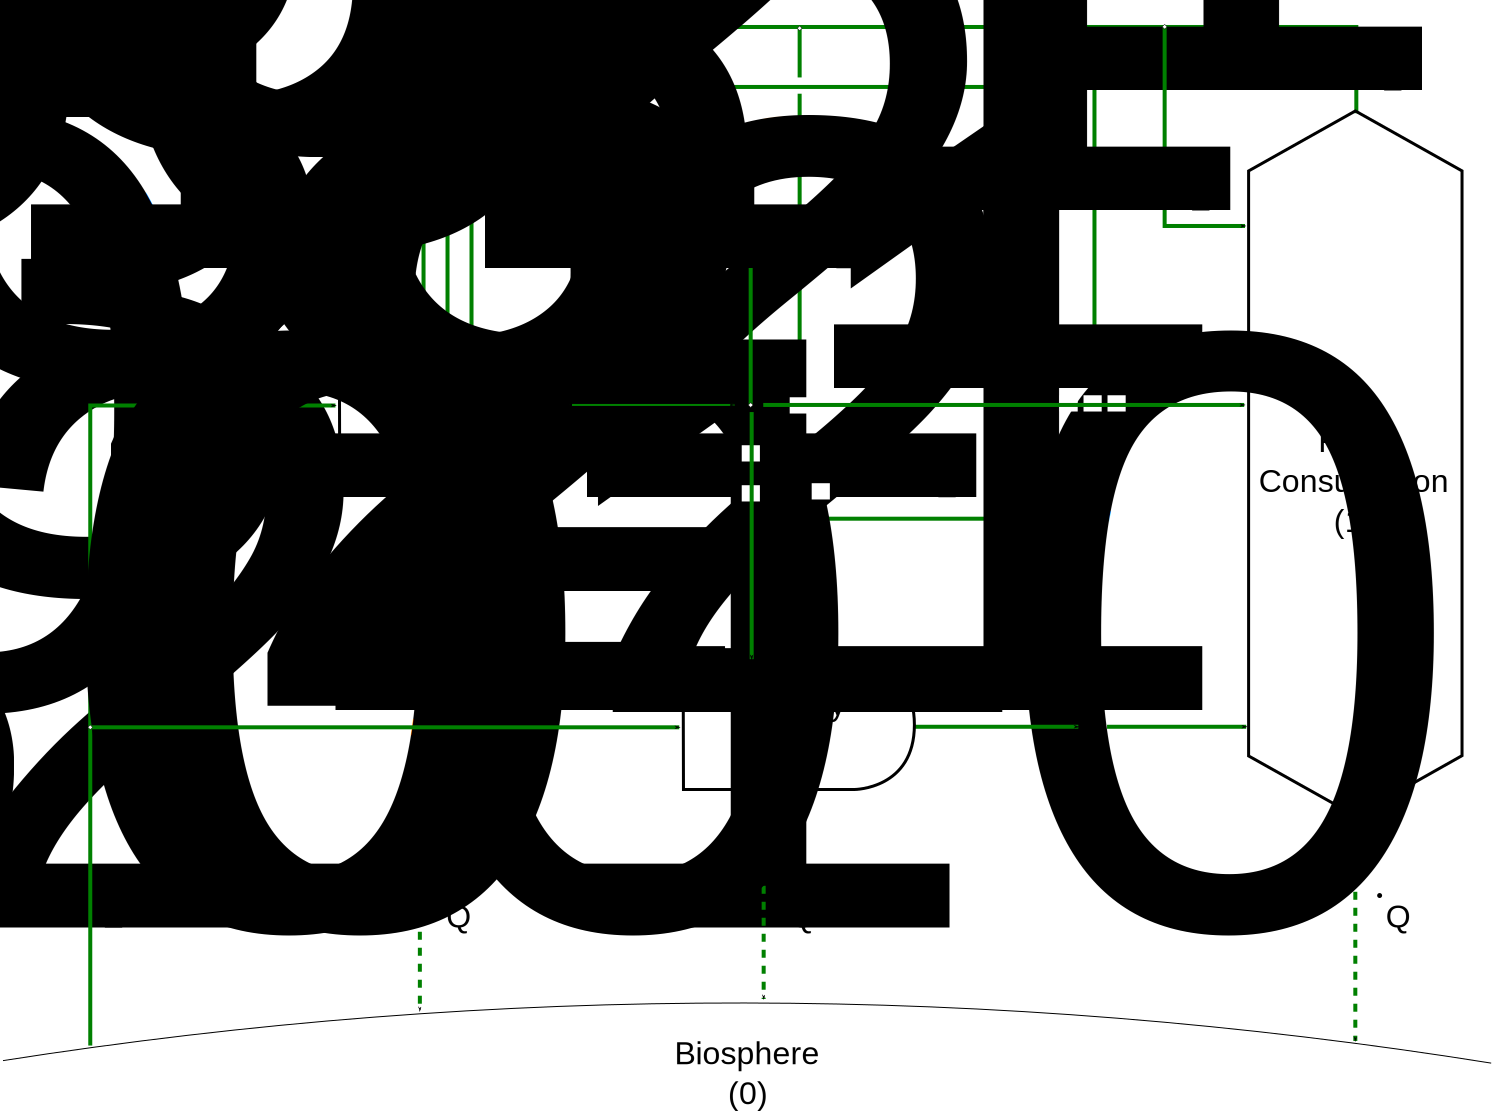
\includegraphics[width=0.8\linewidth]{Part_1/Chapter_Energy/images/3_sector_direct_energy.pdf}
\caption[Direct energy flows for a three-sector economy]{Direct energy flows ($\dot{E}$) for a three-sector economy.}
\label{fig:C_energy}
\end{figure}

The First Law of Thermodynamics around the 
biosphere (0), society (1), and the energy sector (2) gives

\begin{equation} \label{eq:C-CV_E_dot_0}
	\frac{\mathrm{d}E_{0}}{\mathrm{d}t} 	 
	= \dot{Q}_{10} 
	+ \dot{Q}_{20} 
	+ \dot{Q}_{30} 
	- \dot{E}_{02} 
	- \dot{E}_{03},
\end{equation}

\begin{equation} \label{eq:C-CV_E_dot_1}
	\frac{\mathrm{d}E_{1}}{\mathrm{d}t}
	= \dot{E}_{11}
	+ \dot{E}_{21}  
	+ \dot{E}_{31} 
	- \dot{E}_{1}
	- \dot{Q}_{10},
\end{equation}

\noindent and 

\begin{equation} \label{eq:C-CV_E_dot_2}
	\frac{\mathrm{d}E_{2}}{\mathrm{d}t} 	 
	= \dot{E}_{02} 
	+ \dot{E}_{12}
	+ \dot{E}_{22} 
	+ \dot{E}_{32} 
	- \dot{E}_{2} 
	- \dot{Q}_{20}.
\end{equation}

The First Law around the goods and services sector (3) including, 
for now, the accumulation rate of direct energy in the sector 
$\left(\frac{\mathrm{d}E_{3}}{\mathrm{d}t}\right)$ yields

\begin{equation} \label{eq:C-CV_E_dot_3}
	\frac{\mathrm{d}E_{3}}{\mathrm{d}t} 
	= \dot{E}_{03} 
	+ \dot{E}_{13}
	+ \dot{E}_{23} 
	+ \dot{E}_{33} 
	- \dot{E}_3 
	- \dot{Q}_{30}.
\end{equation}

Similar to Example~B, we can generalize 
Equations~\ref{eq:C-CV_E_dot_0}--\ref{eq:C-CV_E_dot_3}
with sums to obtain

\begin{equation} \label{eq:C-CV_E_biosphere_general}
	\frac{\mathrm{d}E_{0}}{\mathrm{d}t} 	 
	= \sum\limits_{i=1}^n \dot{Q}_{i0} - \sum\limits_{i=1}^n \dot{E}_{0i}
\end{equation}

\noindent and

\begin{equation} \label{eq:C-CV_E_econ_general}
	\frac{\mathrm{d}E_{j}}{\mathrm{d}t} 
	= \sum\limits_{i=0}^n\dot{E}_{ij} 
	- \dot{E}_{j}  
	- \dot{Q}_{j0},
\end{equation}

\noindent where $j \in [1, n]$. 
Equations~\ref{eq:C-CV_E_biosphere_general} and 
\ref{eq:C-CV_E_econ_general} are identical to 
Equations~\ref{eq:CV_E_biosphere_general} and 
\ref{eq:B-CV_E_econ_general}, 
indicating that we have successfully generalized 
the model to any number of sectors.

In this economy, the purpose of the goods and services sector (3) 
is to produce goods and provide services, 
it provides no direct energy to society. 
The purpose of the energy sector (2) is to make direct energy ($\dot{E}$) 
available to the economy and society in a useful form.
We may simplify the above equations
by realizing that (a)~$\dot{E}_{3} = \dot{E}_{3i} = 0$, 
because the goods and services sector 
is assumed to produce no direct energy, 
and (b) $\dot{E}_{03} = 0$, 
because the goods and services sector (3) 
receives no direct energy from the biosphere (0), 
except via the energy sector (2).
Thus, several terms in the sums of
Equation~\ref{eq:C-CV_E_econ_general}
will be zero.


%%%%%%%%%% Energy: Auto industry example %%%%%%%%%%
\section{Direct energy in the auto industry}
\label{sec:energy_auto}
%%%%%%%%%%

In this section we discuss inflow of direct energy into the automobile industry
as shown in Figure~\ref{fig:PERKS_energy_auto}.
In 2010, the automobile industry purchased 28 trillion kJ of total energy from all sources. 
Table~\ref{tab:auto_energy} shows the breakdown of energy by source. 

\begin{figure}[!ht]
\centering
\includegraphics[width=0.8\linewidth]{Part_1/Chapter_Energy/images/PERKS_basic_unit_energy_auto_ind.pdf}
\caption[Direct energy flows for the US automobile industry]
{Direct energy flows for the US automobile industry.\cite[Table 7.6]{EIA:2014aa}}
\label{fig:PERKS_energy_auto}
\end{figure}

\begin{table}
\caption[Energy inputs to US auto industry in 2010]{Energy inputs to US auto industry 
(NAICS Code 336111) in 2010.\cite[Table 7.6]{EIA:2014aa}}
\begin{center}
 \begin{tabular}{ r @{\hspace{2em}} l }
\toprule 
Source & Quantity \\
\midrule
Electricity &   $3.0 \times 10^{9}$ kW-hr                    \\
Natural gas &   $1.5 \times 10^{10}$  ft$^{3}$               \\
Other       &   $1.0 \times 10^{12}$  BTU                    \\
\midrule
Total       &   $2.8 \times 10^{13}$ kJ (thermal equivalent) \\
\bottomrule
\end{tabular}
\end{center}
\label{tab:auto_energy}
\end{table}

Total energy use can also be estimated by summing the energy use of the 
underlying detailed processes in manufacturing automobiles. 
Sullivan et al.\ arrive at an estimate of the ``gate-to-gate'' energy
used in the process of creating one automobile (the direct energy used within the
automobile manufacturing process only).\cite{Sullivan2010} 
This estimate can be
mulitplied by the number of vehicles manufactured in a given year 
to obtain total energy use by the 
automobile industry. 
Sullivan estimated a total direct energy use of 34,000 MJ for a generic 1,532 kg vehicle. 
% Using Sullivan's estimate in conjunction with the 19 trillion kJ of total auto industry energy use would suggest that there were
% approximately 560,000 vehicles produced in the US in 2010. (19 million GJ divided by 34 GJ).  That is at least in the ballpark of the estimated 2.7 million actual vehicles produced in 2010.\cite{Motor-Vehicle-Manufacturers-OICA:2014aa}


%%%%%%%%%%  Energy: Summary %%%%%%%%%%
\section{Summary}
\label{sec:energy_summary}
%%%%%%%%%%

In this chapter, we have developed equations, 
assisted by the First Law of Thermodynamics,
that describe the flow of 
direct energy ($\dot{E}$) through economies (Section~\ref{sec:energy_methodology}).
Examples~A--C afforded the opportunity to apply the equations to % chktex 8
model economies with increasing levels of disaggregation
(Sections~\ref{sec:A_energy}--\ref{sec:C_energy}). 
Finally, the energy flows for our running example, the US auto industry,
were discussed in Section~\ref{sec:energy_auto}.

In the next chapter, the direct energy equations developed above will be used to 
develop \emph{embodied} energy accounting equations for Examples~A--C. % chktex 8


\bibliographystyle{unsrt}
\bibliography{../../EROI_review_v2}




% subsection subsection_name (end)


% Always give a unique label
% and use \ref{<label>} for cross-references
% and \cite{<label>} for bibliographic references
% use \sectionmark{}
% to alter or adjust the section heading in the running head
%% Instead of simply listing headings of different levels we recommend to let every heading be followed by at least a short passage of text. Furtheron please use the \LaTeX\ automatism for all your cross-references and citations.

%% Please note that the first line of text that follows a heading is not indented, whereas the first lines of all sequent paragraphs are.

%% Use the standard \verb|equation| environment to typeset your equations, e.g.
%
%% \begin{equation}
%% a \times b = c\;,
%% \end{equation}
%
%% however, for multiline equations we recommend to use the \verb|eqnarray|
%% environment\footnote{In physics texts please activate the class option \texttt{vecphys} to depict your vectors in \textbf{\itshape boldface-italic} type - as is customary for a wide range of physical jects.}.
%% \begin{eqnarray}
%% a \times b = c \nonumber\\
%% \vec{a} \cdot \vec{b}=\vec{c}
%% \label{eq:01}
%% \end{eqnarray}

%% \section{section Heading}
%% \label{sec:2}
%% Instead of simply listing headings of different levels we recommend to let every heading be followed by at least a short passage of text. Furtheron please use the \LaTeX\ automatism for all your cross-references\index{cross-references} and citations\index{citations} as has already been described in Sect.~\ref{sec:2}.

%% \begin{quotation}
%% Please do not use quotation marks when quoting texts! Simply use the \verb|quotation| environment -- it will automatically render Springer's preferred layout.
%% \end{quotation}


%% \section{section Heading}
%% Instead of simply listing headings of different levels we recommend to let every heading be followed by at least a short passage of text. Furtheron please use the \LaTeX\ automatism for all your cross-references and citations as has already been described in Sect.~\ref{sec:2}, see also Fig.~\ref{fig:1}\footnote{If you copy text passages, figures, or tables from other works, you must obtain \textit{permission} from the copyright holder (usually the original publisher). Please enclose the signed permission with the manucript. The sources\index{permission to print} must be acknowledged either in the captions, as footnotes or in a separate section of the book.}

%% Please note that the first line of text that follows a heading is not indented, whereas the first lines of all sequent paragraphs are.

% For figures use
%
%% \begin{figure}[b]
%% \sidecaption
% Use the relevant command for your figure-insertion program
% to insert the figure file.
% For example, with the option graphics use
%% \includegraphics[scale=.65]{figure}
%
% If not, use
%\picplace{5cm}{2cm} % Give the correct figure height and width in cm
%
%% \caption{If the width of the figure is less than 7.8 cm use the \texttt{sidecapion} command to flush the caption on the left side of the page. If the figure is positioned at the top of the page, align the sidecaption with the top of the figure -- to achieve this you simply need to use the optional argument \texttt{[t]} with the \texttt{sidecaption} command}
%% \label{fig:1}       % Give a unique label
%% \end{figure}


%% \paragraph{Paragraph Heading} %
%% Instead of simply listing headings of different levels we recommend to let every heading be followed by at least a short passage of text. Furtheron please use the \LaTeX\ automatism for all your cross-references and citations as has already been described in Sect.~\ref{sec:2}.

%% Please note that the first line of text that follows a heading is not indented, whereas the first lines of all sequent paragraphs are.

%% For typesetting numbered lists we recommend to use the \verb|enumerate| environment -- it will automatically render Springer's preferred layout.

%% \begin{enumerate}
%% \item{Livelihood and survival mobility are oftentimes coutcomes of uneven socioeconomic development.}
%% \begin{enumerate}
%% \item{Livelihood and survival mobility are oftentimes coutcomes of uneven socioeconomic development.}
%% \item{Livelihood and survival mobility are oftentimes coutcomes of uneven socioeconomic development.}
%% \end{enumerate}
%% \item{Livelihood and survival mobility are oftentimes coutcomes of uneven socioeconomic development.}
%% \end{enumerate}


%% \paragraph{paragraph Heading} In order to avoid simply listing headings of different levels we recommend to let every heading be followed by at least a short passage of text. Use the \LaTeX\ automatism for all your cross-references and citations as has already been described in Sect.~\ref{sec:2}, see also Fig.~\ref{fig:2}.

%% Please note that the first line of text that follows a heading is not indented, whereas the first lines of all sequent paragraphs are.

%% For unnumbered list we recommend to use the \verb|itemize| environment -- it will automatically render Springer's preferred layout.

%% \begin{itemize}
%% \item{Livelihood and survival mobility are oftentimes coutcomes of uneven socioeconomic development, cf. Table~\ref{tab:1}.}
%% \begin{itemize}
%% \item{Livelihood and survival mobility are oftentimes coutcomes of uneven socioeconomic development.}
%% \item{Livelihood and survival mobility are oftentimes coutcomes of uneven socioeconomic development.}
%% \end{itemize}
%% \item{Livelihood and survival mobility are oftentimes coutcomes of uneven socioeconomic development.}
%% \end{itemize}

%% \begin{figure}[t]
%% \sidecaption[t]
% Use the relevant command for your figure-insertion program
% to insert the figure file.
% For example, with the option graphics use
%% \includegraphics[scale=.65]{figure}
%
% If not, use
%\picplace{5cm}{2cm} % Give the correct figure height and width in cm
%
%% \caption{Please write your figure caption here}
%% \label{fig:2}       % Give a unique label
%% \end{figure}

%% \runinhead{Run-in Heading Boldface Version} Use the \LaTeX\ automatism for all your cross-references and citations as has already been described in Sect.~\ref{sec:2}.

%% \runinhead{Run-in Heading Italic Version} Use the \LaTeX\ automatism for all your cross-refer\-ences and citations as has already been described in Sect.~\ref{sec:2}\index{paragraph}.
% Use the \index{} command to code your index words
%
% For tables use
%
%% \begin{table}
%% \caption{Please write your table caption here}
%% \label{tab:1}       % Give a unique label
%
% For LaTeX tables use
%
%% \begin{tabular}{p{2cm}p{2.4cm}p{2cm}p{4.9cm}}
%% \hline\noalign{\smallskip}
%% Classes & class & Length & Action Mechanism  \\
%% \noalign{\smallskip}\svhline\noalign{\smallskip}
%% Translation & mRNA$^a$  & 22 (19--25) & Translation repression, mRNA cleavage\\
%% Translation & mRNA cleavage & 21 & mRNA cleavage\\
%% Translation & mRNA  & 21--22 & mRNA cleavage\\
%%Translation & mRNA  & 24--26 & Histone and DNA Modification\\
%%\noalign{\smallskip}\hline\noalign{\smallskip}
%%\end{tabular}
%%$^a$ Table foot note (with superscript)
%%\end{table}
%
%% \section{Section Heading}
%%\label{sec:3}
% Always give a unique label
% and use \ref{<label>} for cross-references
% and \cite{<label>} for bibliographic references
% use \sectionmark{}
% to alter or adjust the section heading in the running head
%% Instead of simply listing headings of different levels we recommend to let every heading be followed by at least a short passage of text. Furtheron please use the \LaTeX\ automatism for all your cross-references and citations as has already been described in Sect.~\ref{sec:2}.

%% Please note that the first line of text that follows a heading is not indented, whereas the first lines of all sequent paragraphs are.

%%If you want to list definitions or the like we recommend to use the Springer-enhanced \verb|description| environment -- it will automatically render Springer's preferred layout.

%%\begin{description}[Type 1]
%%\item[Type 1]{That addresses central themes pertainng to migration, health, and disease. In Sect.~\ref{sec:1}, Wilson discusses the role of human migration in infectious disease distributions and patterns.}
%%\item[Type 2]{That addresses central themes pertainng to migration, health, and disease. In Sect.~\ref{sec:2}, Wilson discusses the role of human migration in infectious disease distributions and patterns.}
%%\end{description}

%%\section{section Heading} %
%% In order to avoid simply listing headings of different levels we recommend to let every heading be followed by at least a short passage of text. Use the \LaTeX\ automatism for all your cross-references and citations citations as has already been described in Sect.~\ref{sec:2}.

%% Please note that the first line of text that follows a heading is not indented, whereas the first lines of all sequent paragraphs are.

%% \begin{svgraybox}
%% If you want to emphasize complete paragraphs of texts we recommend to use the newly defined Springer class option \verb|graybox| and the newly defined environment \verb|svgraybox|. This will produce a 15 percent screened box 'behind' your text.

%% If you want to emphasize complete paragraphs of texts we recommend to use the newly defined Springer class option and environment \verb|svgraybox|. This will produce a 15 percent screened box 'behind' your text.
%% \end{svgraybox}


%% \section{section Heading}
%%Instead of simply listing headings of different levels we recommend to let every heading be followed by at least a short passage of text. Furtheron please use the \LaTeX\ automatism for all your cross-references and citations as has already been described in Sect.~\ref{sec:2}.

%% Please note that the first line of text that follows a heading is not indented, whereas the first lines of all sequent paragraphs are.

%% \begin{theorem}
%% Theorem text goes here.
%% \end{theorem}
%
% or
%
%% \begin{definition}
%% Definition text goes here.
%% \end{definition}

%% \begin{proof}
%\smartqed
%% Proof text goes here.
%% \qed
%% \end{proof}

%%\paragraph{Paragraph Heading} %
%% Instead of simply listing headings of different levels we recommend to let every heading be followed by at least a short passage of text. Furtheron please use the \LaTeX\ automatism for all your cross-references and citations as has already been described in Sect.~\ref{sec:2}.

%% Note that the first line of text that follows a heading is not indented, whereas the first lines of all subsequent paragraphs are.
%
% For built-in environments use
%
%%\begin{theorem}
%%Theorem text goes here.
%%\end{theorem}
%
%%\begin{definition}
%%Definition text goes here.
%%\end{definition}
%
%%\begin{proof}
%%\smartqed
%% Proof text goes here.
%%\qed
%%\end{proof}
%
%% \begin{acknowledgement}
%% If you want to include acknowledgments of assistance and the like at the end of an individual chapter please use the \verb|acknowledgement| environment -- it will automatically render Springer's preferred layout.
%% \end{acknowledgement}
%
%% \section*{Appendix}
%% \addcontentsline{toc}{section}{Appendix}
%
%% When placed at the end of a chapter or contribution (as opposed to at the end of the book), the numbering of tables, figures, and equations in the appendix section continues on from that in the main text. Hence please \textit{do not} use the \verb|appendix| command when writing an appendix at the end of your chapter or contribution. If there is only one the appendix is designated ``Appendix'', or ``Appendix 1'', or ``Appendix 2'', etc. if there is more than one.

%% \begin{equation}
%% a \times b = c
%% \end{equation}
% Problems or Exercises should be sorted chapterwise
%% \section*{Problems}
%% \addcontentsline{toc}{section}{Problems}
%
% Use the following environment.
% Don't forget to label each problem;
% the label is needed for the solutions' environment
%% \begin{prob}
%% \label{prob1}
%% A given problem or Excercise is described here. The
%% problem is described here. The problem is described here.
%% \end{prob}

%% \begin{prob}
%% \label{prob2}
%% \textbf{Problem Heading}\\
%% (a) The first part of the problem is described here.\\
%% (b) The second part of the problem is described here.
%% \end{prob}




%!TEX root = ../../Heun_Dale_Haney_A_dynamic_approach_to_input_output_modeling.tex
%%%%%%%%%%%%%%%%%%%%% chapter.tex %%%%%%%%%%%%%%%%%%%%%%%%%%%%%%%%%
%
% sample chapter
%
% Use this file as a template for your own input.
%
%%%%%%%%%%%%%%%%%%%%%%%% Springer-Verlag %%%%%%%%%%%%%%%%%%%%%%%%%%
%\motto{Use the template \emph{chapter.tex} to style the various elements of your chapter content.}
\motto{One of the main sinks of energy in 
the ``developed'' world is the creation of stuff.
In its natural life cycle, 
stuff passes through three stages. 
First, a new-born stuff is displayed in 
shiny packaging on a shelf in a shop. 
At this stage, stuff is called ``goods.'' 
As soon as the stuff is taken home 
and sheds its packaging, 
it undergoes a transformation from ``good'' 
to its second form, ``clutter.'' 
The clutter lives with its owner for 
a period of months or years. 
During this period, 
the clutter is largely ignored by its owner, 
who is off at the shops buying more goods. 
Eventually, by a miracle of modern alchemy, 
the clutter is transformed into its final form, 
rubbish. **** Should this be ``rubbish.''? ****
To the untrained eye, 
it can be difficult to distinguish this ``rubbish'' 
from the highly desirable ``good'' 
that it used to be. 
Nonetheless, at this stage 
the discerning owner pays the dustman 
to transport the stuff away.\cite[p.88]{Mackay2008}

\hfill---\emph{David MacKay}}

%%%%%%%%%%%%%%%%%%%%%%%%%%%%%%%%%%%%%%%%%%%
%%%%%%%%%% Embodied Energy Flows %%%%%%%%%%
%%%%%%%%%%%%%%%%%%%%%%%%%%%%%%%%%%%%%%%%%%%
\chapter{Embodied energy flows}
% Always give a unique label
\label{chap:embodied_energy}
% use \chaptermark{} to alter or adjust the chapter heading in the running head
\chaptermark{Embodied energy}
%%%%%%%%%%%%%%%%%%%%%%%%%%%%%%%%%%%%%%%%%%%
%%%%%%%%%%%%%%%%%%%%%%%%%%%%%%%%%%%%%%%%%%%
%%%%%%%%%%%%%%%%%%%%%%%%%%%%%%%%%%%%%%%%%%%


\abstract*{[NEED TO ADD ABSTRACT HERE]}

%% \abstract{Each chapter should be preceded by an abstract (10--15 lines long) that summarizes the content. The abstract will appear \textit{online} at \url{www.SpringerLink.com} and be available with unrestricted access. This allows unregistered users to read the abstract as a teaser for the complete chapter. As a general rule the abstracts will not appear in the printed version of your book unless it is the style of your particular book or that of the series to which your book belongs.\newline\indent
%% Please use the 'starred' version of the new Springer \texttt{abstract} command for typesetting the text of the online abstracts (cf. source file of this chapter template \texttt{abstract}) and include them with the source files of your manuscript. Use the plain \texttt{abstract} command if the abstract is also to appear in the printed version of the book.}
%% Use the template \emph{chapter.tex} together with the Springer document class SVMono (monograph-type books) or SVMult (edited books) to style the various elements of your chapter content in the Springer layout.


In Chapter~\ref{chap:direct_energy}, the 
First Law of Thermodynamics\index{First Law of Thermodynamics}
accounted direct energy ($\dot{E}$) flowing among sectors of an economy.
In this chapter, we will adapt the First Law to account  
\emph{embodied} energy\index{embodied energy}\index{energy!embodied|see{embodied energy}}
in the material flows of 
an economy.\footnote{To the authors' knowledge, 
this is the first appearance in the literature 
of a systematic, detailed, and mathematically rigorous derivation 
of embodied energy accounting equations based upon the 
laws of thermodynamics.}

Energy can become ``embodied'' in the output of an economic sector
and within the material in the sector itself.
The energy embodied in the output of an economic sector 
(e.g., energy embodied in the automobiles produced by the automotive sector)
is related to the sum of all direct energy
consumed in the manufacture of its products, 
including all upstream processing stages. 
Embodied energy gives an indication 
of the energy demand created by consumption of goods and services
within an economy.

Energy that becomes embodied in the materials of an economic sector 
(such as the machines, factories, and dealerships 
within the automotive sector itself) is essential for 
the efficient operation of the sector. The amount of energy
embodied in the sector is an indicator of the complexity of
the sector; the amount of energy embodied in an entire economy
can be an indicator of the level of 
economic development\index{economic development}
of the economy.

The purpose of this chapter is to develop a model for 
embodied energy flows within economies. 
With an embodied energy model in hand, we will be positioned
to develop a model for the energy intensity 
of goods and services within an economy 
(Chapter~\ref{chap:intensity}).


%%%%%%%%%% Embodied Energy: Methodology %%%%%%%%%%
\section{Methodology}
\label{sec:embodied_methodology}
%%%%%%%%%%

We begin the derivation of embodied energy accounting
equations by defining the concept of 
\emph{total} energy\index{total energy}\index{energy!total|see{total energy}}. 


%+++++++++ Embodied Energy: Total Energy Accounting ++++++++++
\subsection{Total energy accounting}
\label{sec:total_energy_accounting}
%+++++++++

Total energy ($T$)\nomenclature[T]{$T$}{total energy [J]}
is defined as the sum of 
direct energy\index{direct energy} 
($E$, see Chapter~\ref{chap:direct_energy}) 
and embodied energy ($B$)\nomenclature[B]{$B$}{embodied energy [J]}.

\begin{equation} \label{eq:T_def}
	T \equiv E + B
\end{equation}

The flow rate of total energy 
($\dot{T}$)\nomenclature[T]{$\dot{T}$}{total energy flow rate [W]}
among sectors in 
the economy, the biosphere, and society is the sum of
direct energy ($\dot{E}$) and embodied 
energy ($\dot{B}$)\nomenclature[B]{$\dot{B}$}{embodied energy flow rate [W]}.

\begin{equation} \label{eq:T_dot_def}
	\dot{T} = \dot{E} + \dot{B}
\end{equation}

\noindent Figure~\ref{fig:embodied_single_producer} illustrates
that total energy flows are comprised of
direct energy ($\dot{E}$) and embodied energy ($\dot{B}$). 

\begin{figure}[!ht]
	\centering\
	\includegraphics[width=.9\textwidth]{Part_1/Chapter_Embodied/images/PERKS_basic_unit_embodied_energy_content.pdf}
	\caption[Total energy flows for a single sector]{Total energy flows 
	($\dot{T}$) for a single sector of an economy. 
	For the sake of clarity, 
	direct ($\dot{E}$) and embodied ($\dot{B}$) energy flows
	are shown separately for material inflows from other sectors only.
%	**** I think the red $\dot{B}_{\dot{S}}$ and $\dot{E}_{\dot{S}}$
%	should be changed to $\dot{B}_{\dot{R}}$ and $\dot{E}_{\dot{R}}$. MKH **** MCD - well spotted, Sir! ****
}
\label{fig:embodied_single_producer}
\end{figure}

In some cases, a material flow may include 
either direct energy ($\dot{E}$) 
or embodied energy ($\dot{B}$), exclusive. 
For example, the flow of extracted crude oil from the earth 
consists of direct energy only ($\dot{B} = 0$ and $\dot{T} = \dot{E}$), 
because, in this method, no embodied energy ($B$) is added 
to the crude oil until it reaches the downstream side of the oil rig.
The material produced by a non-energy sector of the economy 
consists of indirect energy only ($\dot{E} \approx 0$, 
and therefore $\dot{T} \approx \dot{B}$), 
because direct energy ($E$) produced by 
a non-energy sector is negligible in this economy. 

In other cases, a material flow may include both direct energy flow
($\dot{E}$) \emph{and} embodied energy flow ($\dot{B}$) components.
For example, the outgoing flow of refined petroleum from the energy sector 
has both a direct energy ($\dot{E}$, the energy content of the oil product, 
usually represented by chemical potential energy) 
and embodied energy ($\dot{B}$, which accounts for the energy 
consumed in upstream processes 
to extract and refine the crude oil).\footnote{Outputs from 
agricultural sectors will be similar: 
both (a) the direct energy component (comprising chemical potential energy) 
and (b) the embodied energy component (representing upstream
energy consumed in food production) will be non-zero.}

Most of the I-O literature~\cite{Bullard1975, Herendeen1978} 
applies the following (and often unstated) assumptions:

\begin{enumerate}
	\item flows of total energy ($\dot{T}$) are 
	\emph{conserved},\footnote{Total energy 
	can be neither created nor destroyed.}

	\item steady state conditions exist 
	(i.e., total energy does not accumulate in economic 
	sectors),\footnote{We will see later how the
	steady-state assumption in the literature 
	can introduce errors into I-O analyses.} and
	
	\item the sum of the signed 
	(input is positive, output is negative) 
	total energy inflows of a sector
	is assigned to the products of the sector (i.e., 
	there is no ``waste'' of total energy).
\end{enumerate}

Like the I-O literature, we assume that total energy is conserved
and never wasted.\footnote{Of course, waste heat exists and is
accounted by the First Law of Thermodynamics. However,
waste heat is ignored when accounting for total energy.}
However, we depart from the I-O literature to allow durability of goods 
as represented by total energy accumulation in economic sectors. 
Steady state, this approach is not. 

Total energy ($T$) may accumulate within an economic sector 
as stocks of direct energy materials 
(piles of coal or tanks of oil) 
but also as energy embodied in stocks of capital goods 
(e.g., machinery or buildings). 
The rate of accumulation of total energy 
in a sector of the economy, the biosphere, 
or society is given by the time derivative of total energy:

\begin{equation} \label{eq:T_accum_def}
	\frac{\mathrm{d}T}{\mathrm{d}t} 
	= \frac{\mathrm{d}E}{\mathrm{d}t} 
	+ \frac{\mathrm{d}B}{\mathrm{d}t}.
\end{equation}

The following equation provides a total energy accounting 
for a sector of the economy, where the $\dot{T}$ terms
are signed: positive for total energy input and negative
for total energy output.

\begin{equation} \label{eq:total_energy_accounting}
		\frac{\mathrm{d}T}{\mathrm{d}t}
		= \sum \dot{T}
\end{equation}

By substituting Equations~\ref{eq:T_dot_def} and
\ref{eq:T_accum_def} into 
Equation~\ref{eq:total_energy_accounting},
we obtain

\begin{equation} \label{eq:total_energy_accounting_details}
	\frac{\mathrm{d}E}{\mathrm{d}t} 
	+ \frac{\mathrm{d}B}{\mathrm{d}t}
	= \sum{\left( \dot{E} 
			+ \dot{B} \right)}.
\end{equation}


%+++++++++ Embodied Energy: Embodied Energy Accounting ++++++++++
\subsection{Embodied energy accounting}
%+++++++++

We note that the definition of total energy 
(Equation~\ref{eq:T_def}) includes direct energy ($E$) 
and embodied energy ($B$) terms. 
On the other hand, the First Law of Thermodynamics 
(Equation~\ref{eq:First_Law_with_accumulation})
includes direct energy ($E$) and waste heat ($Q$) terms. 
The consequence of the foregoing difference is that 
an interesting relationship exists between embodied energy ($B$) 
and waste heat ($Q$), as we shall see below. 

To derive an accounting equation for embodied energy, we substitute the 
First Law of Thermodynamics (Equation~\ref{eq:First_Law_with_accumulation})
into the total energy accounting equation (Equation~\ref{eq:total_energy_accounting_details}).

\begin{equation} \label{eq:embodied_energy_accounting}
	\frac{\mathrm{d}B}{\mathrm{d}t}
	= \sum \dot{B} 
	+ \sum \dot{Q}_{out}
\end{equation}

The waste energy terms ($\dot{Q}_{out}$) 
in Equation~\ref{eq:embodied_energy_accounting}
are \emph{outflows} of energy from the sector. 
The embodied energy 
terms ($\dot{B}$) represent embodied energy of inflows
and outflows of material. Splitting the $\dot{B}$ term
into inflows and outflows and rearranging gives

\begin{equation} \label{eq:embodied_energy_accounting_2}
	\frac{\mathrm{d}B}{\mathrm{d}t}
	= \sum \dot{B}_{in}
	- \sum \dot{B}_{out} 
	+ \sum \dot{Q}_{out}
\end{equation}

In words, the rate of accumulation of embodied energy 
in a sector of the economy 
$\left( \frac{\mathrm{d}B}{\mathrm{d}t} \right)$ 
is equal to the sum of the rates of 
inflow of embodied energy into the sector 
	($\dot{B}_{in}$) 
less the rate of output of embodied energy from the sector 
	($\dot{B}_{out}$) 
\emph{plus} the rate of waste direct energy from the sector 
	($\dot{Q}_{out}$). 
The first two terms on the right side of
Equation~\ref{eq:embodied_energy_accounting_2} are expected: 
accumulation is the difference between inflow and outflow rates. 

Rearranging Equation~\ref{eq:embodied_energy_accounting_2}
yields another version of the embodied energy accounting equation:
one that illuminates issues related to 
stages of growth for an economic sector.

\begin{equation} \label{eq:embodied_energy_accounting_3}
	\frac{\mathrm{d}B}{\mathrm{d}t} 
	+ \sum \dot{B}_{out}
	= \sum \dot{B}_{in}
	+ \sum \dot{Q}_{out}
\end{equation}

\noindent From Equation~\ref{eq:embodied_energy_accounting_3},
we see that incoming embodied energy ($\dot{B}_{in}$) and 
waste heat\footnote{Because we have substituted 
the First Law of Thermodynamics into the total energy accounting equation,
$\dot{Q}_{out}$ becomes a proxy for direct energy consumption by the sector.} 
($\dot{Q}_{out}$) can be used to increase either (a)
the embodied energy within a sector of the economy 
$\left( \frac{\mathrm{d}B}{\mathrm{d}t}  \right)$
or (b) the embodied energy output of a sector of the economy 
($\dot{B}_{out}$), 
depending on decisions by actors 
(firms, households, or the government) 
within the sector. 
If the sector is ``building up'' production capacity, 
much of the incoming embodied energy ($\dot{B}_{in}$)
and direct energy consumption (represented by $\dot{Q}_{out}$)
will be used to increase infrastructure 
(and associated embodied energy, $B$) within the sector, 
and $\frac{\mathrm{d}B}{\mathrm{d}t}$ will be positive.
If, on the other hand, the sector is mature, 
much of the incoming embodied energy ($\dot{B}_{in}$)
and direct energy consumption (represented by $\dot{Q}_{out}$)
will be used for production of goods ($\dot{B}_{out}$).
$\frac{\mathrm{d}B}{\mathrm{d}t}$ will be close to zero.
Equation~\ref{eq:embodied_energy_accounting_2} shows that
an economic sector in decline may experience an outflow 
of embodied energy (via products or depreciation\index{depreciation})
in excess of the sum of 
its embodied energy inflows ($\dot{B}_{in}$)
and direct energy consumption (represented by $\dot{Q}_{out}$),
and $\frac{\mathrm{d}B}{\mathrm{d}t}$ will be negative.

Equations~\ref{eq:embodied_energy_accounting_2}
and~\ref{eq:embodied_energy_accounting_3} 
highlight a contrast between 
the present dynamic analysis and the I-O literature.
The traditional assumption of steady-state conditions 
in economic sectors is tantamount to assuming that
$\frac{\mathrm{d}B}{\mathrm{d}t} = 0$ in 
Equations~\ref{eq:embodied_energy_accounting_2}
and~\ref{eq:embodied_energy_accounting_3}.
That assumption precludes analysis of stages of growth 
and the embodied energy implications thereof.

Equations~\ref{eq:embodied_energy_accounting_2}
and~\ref{eq:embodied_energy_accounting_3} 
are generalized embodied energy accounting equations that we will
see again for Examples~A-C in the sections that follow.


%%%%%%%%%% Embodied Energy: Example A %%%%%%%%%%
\section{Example A: single-sector economy} % chktex 13
%%%%%%%%%%

Figure~\ref{fig:A_total_energy_T_dot} shows the flows 
of total energy ($\dot{T}$) through the single-sector economy.

\begin{figure}[!ht]
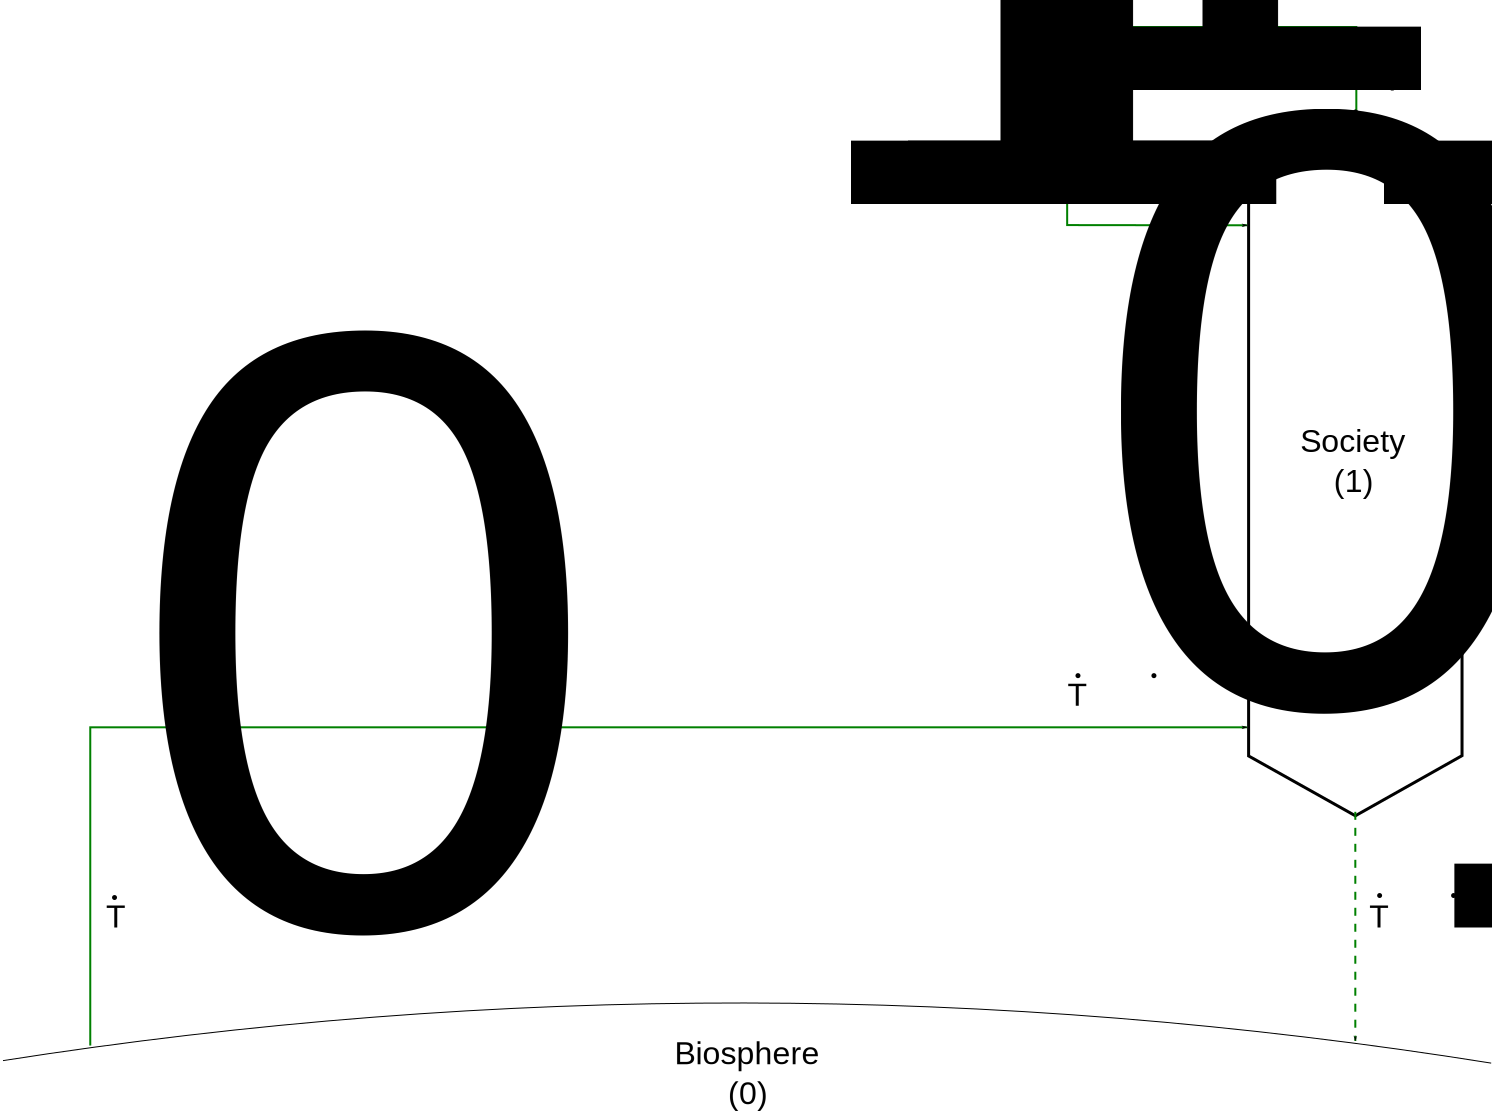
\includegraphics[width=1.0\linewidth]{Part_1/Chapter_Embodied/images/1_sector_embodied_energy.pdf}
\caption[Total energy flows in a one-sector economy]{Total energy flows ($\dot{T}$) in a one-sector economy.}
\label{fig:A_total_energy_T_dot}
\end{figure}

As discussed above, we follow the I-O literature in assuming that 
total energy ($T$) is conserved. 
A total energy accounting around the biosphere (0)
and the single-sector economy (1) gives

\begin{equation} \label{eq:A_T_acct_0}
	\frac{\mathrm{d}T_{0}}{\mathrm{d}t} 
	= \dot{T}_{10} 
	- \dot{T}_{01},
\end{equation}

\noindent and

\begin{equation} \label{eq:A_T_acct_1}
	\frac{\mathrm{d}T_{1}}{\mathrm{d}t} 
	= \dot{T}_{01} 
	+ \dot{T}_{11}
	- \dot{T}_{1}
	- \dot{T}_{10}.
\end{equation}

Substituting Equations~\ref{eq:T_dot_def} and
\ref{eq:T_accum_def} into 
Equations~\ref{eq:A_T_acct_0} and~\ref{eq:A_T_acct_1}
yields

\begin{equation} \label{eq:A_total_energy_0}
	\frac{\mathrm{d}E_{0}}{\mathrm{d}t} 
	+ \frac{\mathrm{d}B_{0}}{\mathrm{d}t} 
	= \dot{E}_{10} 
	+ \dot{B}_{10} 
	- \dot{E}_{01}
	- \dot{B}_{01}
\end{equation}

\noindent and

\begin{equation} \label{eq:A_total_energy_1}
	\frac{\mathrm{d}E_{1}}{\mathrm{d}t} 
	+ \frac{\mathrm{d}B_{1}}{\mathrm{d}t} 
	= \dot{E}_{01} 
	+ \dot{B}_{01} 
	+ \dot{E}_{11}
	+ \dot{B}_{11}
	- \dot{E}_{1}
	- \dot{B}_{1}
	- \dot{E}_{10}
	- \dot{B}_{10}.	
\end{equation}

At this point, we can proceed in two directions.
The first direction, 
simplifying Equations~\ref{eq:A_total_energy_0} 
and~\ref{eq:A_total_energy_1}, 
provides an intuitive result. 
The second direction,
substituting the First Law of Thermodynamics into 
Equations~\ref{eq:A_total_energy_0} 
and~\ref{eq:A_total_energy_1}, 
provides the advantage of cancelling most of the direct energy terms.
We begin with the first approach: simplification.


%+++++++++ Simplified embodied energy ++++++++++
\subsection{Simplification of the embodied energy accounting equation} % (fold)
\label{sec:A_simplified_embodied}
%+++++++++

To simplify Equations~\ref{eq:A_total_energy_0} 
and~\ref{eq:A_total_energy_1},
we first realize that, by definition, no embodied energy flows from 
the earth with extracted material, so $\dot{B}_{01} = 0$
and $\dot{T}_{0} = \dot{E}_{01}$ as shown in Figure~\ref{fig:A_total_energy_T_dot}.
Second, we can assume that direct energy ($E$) does not accumulate
in the economy such that 
$\frac{\mathrm{d}E_0}{\mathrm{d}t} = 0$ and
$\frac{\mathrm{d}E_1}{\mathrm{d}t} = 0$.
Finally, we note that $\dot{E}_{10} = 0$, 
because society does not supply direct energy 
to the biosphere. Thus, Equations~\ref{eq:A_total_energy_0}
and~\ref{eq:A_total_energy_1} become

\begin{equation} \label{eq:A_total_energy_0_simp}
	\frac{\mathrm{d}B_{0}}{\mathrm{d}t} 
	= \dot{B}_{10} 
	- \dot{E}_{01}
\end{equation}

\noindent and

\begin{equation} \label{eq:A_total_energy_1_simp}
	\frac{\mathrm{d}B_{1}}{\mathrm{d}t} 
	= \dot{E}_{01} 
	+ \dot{E}_{11}
	+ \dot{B}_{11}
	- \dot{E}_{1}
	- \dot{B}_{1}
	- \dot{B}_{10}.	
\end{equation}

These equations show that direct energy consumed by a 
sector ($\dot{E}_{01}$) increases the energy embodied within the sector ($B_1$), 
whereas the waste from the sector produces an embodied
energy outflow ($\dot{B}_{10}$) that reduces 
the energy embodied within the sector. 


%+++++++++ First Law embodied energy ++++++++++
\subsection{Substitution of First Law into the embodied energy accounting equation} % (fold)
\label{subsec:A_first_law_embodied}
%+++++++++

The second approach to the derivation of embodied energy
accounting equations is to substitute the First Law
(Equations~\ref{eq:dE_0/dt_single_sector} and~\ref{eq:dE_1/dt_single_sector}) 
into the total energy accounting equations 
(Equations~\ref{eq:A_total_energy_0} and~\ref{eq:A_total_energy_1}). 
\begin{equation} \label{eq:A_dB0/dt}
	\frac{\mathrm{d}B_{0}}{\mathrm{d}t} 
	= \dot{E}_{10}
	+ \dot{B}_{10} 
	- \dot{B}_{01}
	- \dot{Q}_{10}
\end{equation}

\begin{equation} \label{eq:A_dB1/dt}
	\frac{\mathrm{d}B_{1}}{\mathrm{d}t} 
	= \dot{B}_{01} 
	+ \dot{B}_{11}
	- \dot{B}_{1}
	- \dot{B}_{10}
	- \dot{E}_{10}
	+ \dot{Q}_{10}
\end{equation}

This substitution has the advantage of canceling most 
of the direct energy terms from the embodied energy accounting equations.
And, it is no longer necessary to assume that the 
accumulation rate of direct energy 
$\left( \frac{\mathrm{d}E}{\mathrm{d}t} \right)$
is zero, because the 
$\frac{\mathrm{d}E}{\mathrm{d}t}$
term is cancelled by the substitution.

Note that the Equation~\ref{eq:A_dB0/dt} includes the
term $-\dot{Q}_{10}$, which, at first glance,
appears different from 
Equation~\ref{eq:embodied_energy_accounting_2}.\footnote{Equation~\ref{eq:embodied_energy_accounting_2}
has a positive sign for the waste energy term (+ $\dot{Q}_{out}$),
whereas Equation~\ref{eq:A_dB0/dt} has a 
negative sign for the waste energy term ($- \dot{Q}_{10}$).}
However, upon realizing that $\dot{Q}_{10}$ is an \emph{inflow}
of waste energy into the biosphere, we can use $\dot{Q}_{10} = - \dot{Q}_{01}$
to rewrite Equation~\ref{eq:A_dB0/dt} with an \emph{outflow} 
term,

\begin{equation} \label{eq:A_dB0/dt_waste_outflow}
	\frac{\mathrm{d}B_{0}}{\mathrm{d}t} 
	= \dot{E}_{10}
	+ \dot{B}_{10} 
	- \dot{B}_{01}
	+ \dot{Q}_{01},
\end{equation}

\noindent thereby maintining consistency with
Equation~\ref{eq:embodied_energy_accounting_2}.

We can simplify 
Equations~\ref{eq:A_dB0/dt} and~\ref{eq:A_dB1/dt} 
using the assumptions of Section~\ref{sec:A_simplified_embodied} 
(namely, that $\dot{B}_{01} = 0$ and $\dot{E}_{10} = 0$)
to obtain

\begin{equation} \label{eq:A_dB0/dt_simp}
	\frac{\mathrm{d}B_{0}}{\mathrm{d}t} 
	= \dot{B}_{10} 
	- \dot{Q}_{10}
\end{equation}

\noindent and

\begin{equation} \label{eq:A_dB1/dt_simp_prelim}
	\frac{\mathrm{d}B_{1}}{\mathrm{d}t} 
	= \dot{B}_{11}
	- \dot{B}_{1}
	- \dot{B}_{10}
	+ \dot{Q}_{10}.
\end{equation}

\noindent{}The material model of this framework (see Chapter~\ref{chap:materials})
indicates that materials are comprised of 
resources ($R$), 
short-lived materials ($S$), and
capital ($K$).
Thus, we can write 

\begin{equation}
	\frac{\mathrm{d}B_{1}}{\mathrm{d}t} 
	= \frac{\mathrm{d}B_{R,1}}{\mathrm{d}t} 
	+ \frac{\mathrm{d}B_{S,1}}{\mathrm{d}t} 
	+ \frac{\mathrm{d}B_{K,1}}{\mathrm{d}t},
\end{equation}

\noindent{}but neither resources ($R$) nor short-lived
materials ($S$) accumulate in economic sectors at a significant rate.
Thus, 

\begin{equation} \label{eq:A-dBdt_simplification}
	\frac{\mathrm{d}B_{1}}{\mathrm{d}t} 
	= \frac{\mathrm{d}B_{K_{1}}}{\mathrm{d}t}.
\end{equation}

\noindent{}We can substitute Equation~\ref{eq:A-dBdt_simplification}
into Equation~\ref{eq:A_dB1/dt_simp_prelim} to obtain

\begin{equation} \label{eq:A_dB1/dt_simp}
	\frac{\mathrm{d}B_{K,1}}{\mathrm{d}t}
	= \dot{B}_{11}
	- \dot{B}_{1}
	- \dot{B}_{10}
	+ \dot{Q}_{10}.
\end{equation}

\noindent{}Equations~\ref{eq:A_dB0/dt_simp} and~\ref{eq:A_dB1/dt_simp} are 
the embodied energy accounting equations for Example~A.

In Examples~B and C following, we will choose the approach of 
this section, namely substitution of the 
First Law of Thermodynamics into the total energy accounting equation
(instead of simplifying the total energy equation 
as discussed in Section~\ref{sec:A_simplified_embodied}),
because of the benefit of canceling direct energy flow terms ($\dot{E}$). 


%+++++++++ Depreciation ++++++++++
\subsection{Physical depreciation}\index{depreciation}
\label{sec:depreciation_embodied}
%+++++++++

The term $\dot{B}_{10}$ in Equation~\ref{eq:A_dB1/dt_simp}
represents the disposal rate 
of embodied energy from Society (1) to the Biosphere (0). 
Figure~\ref{fig:A_materials} shows that the outgoing material flow
from Society (1) is comprised of 
resources ($\dot{R}_{10}$),
short-lived materials ($\dot{S}_{10}$), and 
capital ($\dot{K}_{10}$). 
Each of these material flows will have associated embodied energy such that

\begin{equation} \label{eq:A-depreciation-of-B}
	\dot{B}_{10}
	= \dot{B}_{\dot{R}_{10}}
	+ \dot{B}_{\dot{S}_{10}}
	+ \dot{B}_{\dot{K}_{10}}.
\end{equation}

The term $\dot{B}_{\dot{K}_{10}}$ represents the energy embodied
in depreciated phyiscal assets.
Physical depreciation\index{depreciation!physical} 
is counted at the moment when material physically departs an economic sector 
and enters the biosphere, presumably a landfill, 
where the material in the wasted assets will decay.
Financial depreciation\index{depreciation!financial}
is usually faster than physical depreciation
according to rates set by accounting rules.
The embodied energy associated with physical depreciation ($\dot{B}_{\dot{K}_{10}}$)
can be represented by a depreciation term such as

\begin{equation} \label{eq:depreciation_term_defined}
	\dot{B}_{\dot{K}_{10}} 
	= \gamma_{B,1} B_{K_{1}},
\end{equation}

\noindent{}where $\gamma_{B}$ represents the depreciation rate 
of embodied energy in units of inverse time (e.g., 1/year) 
with $\gamma_{B} > 0$.\footnote{Note that $\gamma_B$ will, in general,
be different from $\gamma_{K}$ defined in Section~\ref{sec:A_materials}.
$\gamma_{B}$ will equal $\gamma_{K}$ if and only if 
the depreciated capital has an embodied energy content that is 
identical to the average embodied energy content 
of the sector on a per-unit-mass basis.}
The depreciation rate ($\gamma_{B}$) indicates that 
a fraction of the energy embodied in capital stock
is disposed over a period of time (e.g., $\gamma_{B} = 0.05$/year). 
In the absence of other inputs or outputs, 
this depreciation function provides exponential decay 
of embodied energy ($B$) in an economic sector. 
$\gamma_{B}$ is, in general, a function of time.

Equation~\ref{eq:depreciation_term_defined} can be substituted into
Equation~\ref{eq:A-depreciation-of-B} to obtain

\begin{equation} \label{eq:B_10_term}
	\dot{B}_{10}
	= \dot{B}_{\dot{R}_{10}}
	+ \dot{B}_{\dot{S}_{10}}
	+ \gamma_{B,1} B_{K_{1}}.	
\end{equation}

\noindent{}Equation~\ref{eq:B_10_term} 
can be substituted into Equations~\ref{eq:A_dB0/dt_simp}
and~\ref{eq:A_dB1/dt_simp} to obtain 

\begin{equation} \label{eq:A-dB0/dt_with_depreciation_gamma}
	\frac{\mathrm{d}B_{0}}{\mathrm{d}t} 
	= \dot{B}_{\dot{R}_{10}}
	+ \dot{B}_{\dot{S}_{10}}
	+ \gamma_{B,1} B_{K_{1}}
	- \dot{Q}_{10} 
\end{equation}

\noindent{}and

\begin{equation} \label{eq:A-dB1/dt_with_depreciation_gamma}
	\frac{\mathrm{d}B_{K_{1}}}{\mathrm{d}t} 
	= \dot{B}_{11}
	- \dot{B}_{1}
	- \dot{B}_{\dot{R}_{10}}
	- \dot{B}_{\dot{S}_{10}}
	- \gamma_{B,1} B_{K_{1}}
	+ \dot{Q}_{10}.
\end{equation}

\noindent{}Equation~\ref{eq:A-dB1/dt_with_depreciation_gamma} 
indicates that the accumulation rate 
of embodied energy in an economic sector 
$\left( \frac{\mathrm{d}B_{K_{1}}}{\mathrm{d}t} \right)$
is equal to the sum of the embodied energy input to the sector~($\dot{B}_{11}$)
and waste heat from the economic sector~($\dot{Q}_{10}$),
less embodied energy the leaves the sector in its products~($\dot{B}_{1}$), 
less the rate of disposal of embodied energy associated with 
scrap resources~($\dot{B}_{\dot{R}_{10}}$),
short-lived material~($\dot{B}_{\dot{S}_{10}}$), and
depreciated capital stock~($\gamma_{B,1} B_{K_{1}}$).

We turn now to Example~B, a two-sector economy.


%%%%%%%%%% Embodied Energy: Example B %%%%%%%%%%
\section{Example B: two-sector economy} % chktex 13
\label{sec:Embodied_Energy_Example_B}
%%%%%%%%%%

For the two-sector economy of Figures~\ref{fig:B_materials}
and~\ref{fig:B_energy}, we again follow the I-O literature 
by assuming that total energy ($T$) is conserved. 
Figure~\ref{fig:B_total_energy} shows total energy
flows for the two-sector economy.

\begin{figure}[!ht]
\includegraphics[width=0.9\linewidth]{Part_1/Chapter_Embodied/images/2_sector_embodied_energy.pdf}
\caption[Flows of total energy in a two-sector economy.]{Flows of total energy ($\dot{T}$) in a two-sector economy.}
\label{fig:B_total_energy}
\end{figure}

Accounting for accumulation of total energy and using the assumption 
that total energy is conserved, we can write the following equations.

\begin{equation} \label{eq:CV_T_0}
	\frac{\mathrm{d}T_{0}}{\mathrm{d}t} 	 
	= \dot{T}_{10} 
	+ \dot{T}_{20} 
	- \dot{T}_{02},
\end{equation}

\begin{equation} \label{eq:CV_T_1}
	\frac{\mathrm{d}T_{1}}{\mathrm{d}t} 	 
	= \dot{T}_{11}
	+ \dot{T}_{21} 
	- \dot{T}_{1}
	- \dot{T}_{10},
\end{equation}

\noindent and

\begin{equation} \label{eq:CV_T_2}
	\frac{\mathrm{d}T_{2}}{\mathrm{d}t} 	 
	= \dot{T}_{02} 
	+ \dot{T}_{12}
	+ \dot{T}_{22} 
	- \dot{T}_{2} 
	- \dot{T}_{20}.
\end{equation}

Substituting Equations~\ref{eq:T_dot_def} 
and~\ref{eq:T_accum_def} into 
Equations~\ref{eq:CV_T_0} through
\ref{eq:CV_T_2} gives

\begin{equation} \label{eq:CV_dB_0}
	\frac{\mathrm{d}B_{0}}{\mathrm{d}t} 
	+ \frac{\mathrm{d}E_{0}}{\mathrm{d}t} 
	= \dot{E}_{10} 
	+ \dot{B}_{10} 
	+ \dot{E}_{20} 
	+ \dot{B}_{20} 
	- \dot{E}_{02} 
	- \dot{B}_{02},
\end{equation}

\begin{equation} \label{eq:CV_dB_1}
	\frac{\mathrm{d}B_{1}}{\mathrm{d}t} 
	+ \frac{\mathrm{d}E_{1}}{\mathrm{d}t} 
	= \dot{E}_{11}
	+ \dot{B}_{11}
	+ \dot{E}_{21} 
	+ \dot{B}_{21} 
	- \dot{E}_1
	- \dot{B}_1
	- \dot{E}_{10} 
	- \dot{B}_{10},
\end{equation}

\noindent and 

\begin{equation} \label{eq:CV_dB_2}
	\frac{\mathrm{d}B_{2}}{\mathrm{d}t} 
	+ \frac{\mathrm{d}E_{2}}{\mathrm{d}t} 
	= \dot{E}_{02} 
	+ \dot{B}_{02} 
	+ \dot{E}_{12}
	+ \dot{B}_{12}
	+ \dot{E}_{22} 
	+ \dot{B}_{22} 
	- \dot{E}_{2} 
	- \dot{B}_{2} 
	- \dot{E}_{20} 
	- \dot{B}_{20}.
\end{equation}

As in Example~A, we can substitute the First Law of Thermodynamics 
(Equations~\ref{eq:CV_E_dot_0}--\ref{eq:CV_E_dot_2})
into the total energy accounting equations
(Equations~\ref{eq:CV_dB_0}--\ref{eq:CV_dB_2}) 
and employ the assumptions that 
$\dot{E}_{i0} = 0$ and
$\dot{B}_{0j} = 0$ 
to obtain

\begin{equation} \label{eq:B_embodied_energy_accounting_0}
	\frac{\mathrm{d}B_{0}}{\mathrm{d}t} 
	= \dot{B}_{10} 
	+ \dot{B}_{20} 
	- \dot{Q}_{10} 
	- \dot{Q}_{20}, 
\end{equation}

\begin{equation} \label{eq:B_embodied_energy_accounting_1}
	\frac{\mathrm{d}B_{1}}{\mathrm{d}t} 
	= \dot{B}_{11} 
	+ \dot{B}_{21}
	- \dot{B}_{2} 
	- \dot{B}_{10}
	+ \dot{Q}_{10},
\end{equation}

\noindent and

\begin{equation} \label{eq:B_embodied_energy_accounting_2}
	\frac{\mathrm{d}B_2}{\mathrm{d}t} 
	= \dot{B}_{12} 
	+ \dot{B}_{22} 
	- \dot{B}_{2}
	- \dot{B}_{20} 
	+ \dot{Q}_{20}.
\end{equation}

Similar to Example~A, we observe that the accumulation rate 
of embodied energy in the economic sectors (1 and 2) 
is the sum of the rates of waste heat flowing from the sector 
($\dot{Q}_{20}$) and embodied energy into the sector 
($\dot{B}_{12} + \dot{B}_{22}$) 
less the rate of embodied energy leaving the sector 
on its output streams ($\dot{B}_{2} + \dot{B}_{20}$).

Equations~\ref{eq:B_embodied_energy_accounting_0}--\ref{eq:B_embodied_energy_accounting_2}
can be simplified using sums:

\begin{equation} \label{eq:B_embodied_energy_accounting_0_sum}
	\frac{\mathrm{d}B_{0}}{\mathrm{d}t} 
	= \sum\limits_{i=1}^n\dot{B}_{i0} 
	- \sum\limits_{i=1}^n\dot{Q}_{i0} 
\end{equation}

\noindent and

\begin{equation} \label{eq:B_embodied_energy_accounting_12_sum}
	\frac{\mathrm{d}B_{j}}{\mathrm{d}t} 
	= \sum\limits_{i=1}^n\dot{B}_{ij} 
	- \dot{B}_{j}
	- \dot{B}_{j0} 
	+ \dot{Q}_{j0},
\end{equation}

\noindent where $j \in [1, n]$.

As in Example~A, 
we can disaggregate the accumulation and waste embodied energy terms 
and express physical waste of capital stock as depreciation 
in Equations~\ref{eq:B_embodied_energy_accounting_0_sum}
and~\ref{eq:B_embodied_energy_accounting_12_sum}
to obtain

\begin{equation} \label{eq:B_embodied_energy_accounting_0_with_depreciation}
	\frac{\mathrm{d}B_{0}}{\mathrm{d}t} 
	= \sum\limits_{i=1}^n 
		\left( \dot{B}_{\dot{R}_{i0}} 
				+ \dot{B}_{\dot{S}_{i0}} 
				+ \gamma_{B,i} B_{K_{i}} \right)
	- \sum\limits_{i=1}^n\dot{Q}_{i0} 
\end{equation}

\noindent and

\begin{equation} \label{eq:B_embodied_energy_accounting_12_with_depreciation}
	\frac{\mathrm{d}B_{K,j}}{\mathrm{d}t} 
	= \sum\limits_{i=1}^n\dot{B}_{ij} 
	- \dot{B}_{j}
	- \left( \dot{B}_{\dot{R}_{j0}}
		+ \dot{B}_{\dot{S}_{j0}}
		+ \gamma_{B,j} B_{K_{j}} \right)
	+ \dot{Q}_{j0}.
\end{equation}

In the next section, we apply embodied energy accounting to 
Example~C, a three-sector economy.


%%%%%%%%%% Embodied Energy: Example C %%%%%%%%%%
\section{Example C: three-sector economy} % chktex 13
\label{sec:Embodied_Energy_Example_C}
%%%%%%%%%%

Again, we begin with the diagram showing total energy ($\dot{T}$) flows
among the economic sectors of Example~C (Figure~\ref{fig:C_total_energy}).

\begin{figure}[!ht]
\includegraphics[width=1.0\linewidth]{Part_1/Chapter_Embodied/images/3_sector_embodied_energy.pdf}
\caption[Flows of total energy in a three-sector economy.]{Flows of total energy ($\dot{T}$) in a three-sector economy.}
\label{fig:C_total_energy}
\end{figure}

Accounting for accumulation of total energy and 
applying the assumption that total energy is conserved, 
we can write the following equations.
We build from the derivation in Section~\ref{sec:Embodied_Energy_Example_B}
and utilize sums for each equation below.

\begin{equation} \label{eq:C-CV_T_0}
	\frac{\mathrm{d}T_{0}}{\mathrm{d}t} 	 
	= \sum\limits_{i=1}^{n} \dot{T}_{i0}
	- \sum\limits_{j=1}^{n} \dot{T}_{0j}
\end{equation}

\noindent and

\begin{equation} \label{eq:C-CV_T_123}
	\frac{\mathrm{d}T_{j}}{\mathrm{d}t} 	 
	= \sum\limits_{i=0}^{n} \dot{T}_{ij}
	- \dot{T}_{j}
	- \dot{T}_{j0}.
\end{equation}

\noindent where $j \in [1, n]$.

Substituting Equations~\ref{eq:T_dot_def} 
and~\ref{eq:T_accum_def} into 
Equations~\ref{eq:C-CV_T_0} and
\ref{eq:C-CV_T_123} gives

\begin{equation} \label{eq:C-CV_dB_0}
	\frac{\mathrm{d}E_{0}}{\mathrm{d}t}
	+ \frac{\mathrm{d}B_{0}}{\mathrm{d}t} 	 
	= \sum\limits_{i=1}^{n} \dot{E}_{i0}
	+ \sum\limits_{i=1}^{n} \dot{B}_{i0}
	- \sum\limits_{j=1}^{n} \dot{E}_{0j}
	- \sum\limits_{j=1}^{n} \dot{B}_{0j}
\end{equation}

\noindent and

\begin{equation} \label{eq:C-CV_dB_123}
	\frac{\mathrm{d}E_{j}}{\mathrm{d}t}
	+ \frac{\mathrm{d}B_{j}}{\mathrm{d}t} 	 
	= \sum\limits_{i=0}^{n} \dot{E}_{ij}
	+ \sum\limits_{i=0}^{n} \dot{B}_{ij}
	- \dot{E}_{j}
	- \dot{B}_{j}
	- \dot{E}_{j0}
	- \dot{B}_{j0}.
\end{equation}

Substituting the First Law of Thermodynamics 
(Equations~\ref{eq:C-CV_E_biosphere_general} and~\ref{eq:C-CV_E_econ_general}) 
into the total energy accounting equations 
(Equations~\ref{eq:C-CV_dB_0} and~\ref{eq:C-CV_dB_123}) 
and recognizing that $\dot{B}_{0j} = 0$ for $j \in [1, n]$
and $\dot{E}_{i0} = 0$ for $i \in [1, n]$
gives embodied energy accounting equations for Example~C: % chktex 13

\begin{equation} \label{eq:C-embodied_acct_0}
	\frac{\mathrm{d}B_{0}}{\mathrm{d}t} 	 
	= \sum\limits_{i=1}^{n} \dot{B}_{i0}
	- \sum\limits_{i=1}^{n} \dot{Q}_{i0}
\end{equation}

\begin{equation} \label{eq:C-embodied_acct_123}
	\frac{\mathrm{d}B_{j}}{\mathrm{d}t} 	 
	= \sum\limits_{i=0}^{n} \dot{B}_{ij}
	- \dot{B}_{j}
	- \dot{B}_{j0}
	+ \dot{Q}_{j0} 
\end{equation}

As in Example~B, 
we can disaggregate the accumulation and waste embodied energy terms 
and express physical waste of capital stock as depreciation 
in Equations~\ref{eq:C-embodied_acct_0}
and~\ref{eq:C-embodied_acct_123}
to obtain

\begin{equation} \label{eq:C_embodied_energy_accounting_0_with_depreciation}
	\frac{\mathrm{d}B_{0}}{\mathrm{d}t} 
	= \sum\limits_{i=1}^n 
		\left( \dot{B}_{\dot{R}_{i0}} 
				+ \dot{B}_{\dot{S}_{i0}} 
				+ \gamma_{B,i} B_{K_{i}} \right)
	- \sum\limits_{i=1}^n\dot{Q}_{i0} 
\end{equation}

\noindent and

\begin{equation} \label{eq:C_embodied_energy_accounting_123_with_depreciation}
	\frac{\mathrm{d}B_{K_{j}}}{\mathrm{d}t} 
	= \sum\limits_{i=1}^n\dot{B}_{ij} 
	- \dot{B}_{j}
	- \left( \dot{B}_{\dot{R}_{j0}}
		+ \dot{B}_{\dot{S}_{j0}}
		+ \gamma_{B,j} B_{K_{j}} \right)
	+ \dot{Q}_{j0}.
\end{equation}

\noindent which are the same as 
Equations~\ref{eq:B_embodied_energy_accounting_0_with_depreciation}
and~\ref{eq:B_embodied_energy_accounting_12_with_depreciation},
indicating that we have successfully generalized the embodied energy
equations to an arbitrarily-large economy.

To verify the above derivation, 
we sum 
Equations~\ref{eq:C_embodied_energy_accounting_0_with_depreciation} 
and~\ref{eq:C_embodied_energy_accounting_123_with_depreciation} 
for all sectors of the economy $\left( j \in [1,n] \right)$ to obtain

\begin{equation} \label{eq:C_big_sums}
	\begin{split}
		\frac{\mathrm{d}B_{0}}{\mathrm{d}t} 
		+ \sum\limits_{j=1}^n \frac{\mathrm{d}B_{K_{j}}}{\mathrm{d}t} 
		= & 
		 \sum\limits_{i=1}^n 
			\left( \dot{B}_{\dot{R}_{i0}} 
					+ \dot{B}_{\dot{S}_{i0}} 
					+ \gamma_{B,i} B_{K,i} \right)
		- \sum\limits_{i=1}^n \dot{Q}_{i0} \\
		& + \sum\limits_{j=1}^n \sum\limits_{i=1}^n \dot{B}_{ij}
		- \sum\limits_{j=1}^n \dot{B}_{j}	\\
		& - \sum\limits_{j=1}^n
				\left( \dot{B}_{\dot{R}_{j0}}
					+ \dot{B}_{\dot{S}_{j0}}
					+ \gamma_{B,j} B_{K,j} \right)
		+ \sum\limits_{j=1}^n \dot{Q}_{j0}.
	\end{split}
\end{equation}

\noindent{}Using the identities

\begin{equation} \label{eq:B_identity_1}
	\dot{B}_{j}  
	= \sum\limits_{k=1}^n \dot{B}_{jk},
\end{equation} \nomenclature[k]{$k$}{economic sector index}

\noindent{}and

\begin{equation} \label{eq:B_identity_2}
	\sum\limits_{j=1}^n\dot{B}_{j}  
	= \sum\limits_{j=1}^n \sum\limits_{k=1}^n \dot{B}_{jk}
	= \sum\limits_{i=1}^n \sum\limits_{k=1}^n \dot{B}_{ik}
	= \sum\limits_{i=1}^n \sum\limits_{j=1}^n \dot{B}_{ij}
	= \sum\limits_{j=1}^n \sum\limits_{i=1}^n \dot{B}_{ij},
\end{equation}

\noindent{}Equation~\ref{eq:C_big_sums} becomes

\begin{equation} \label{eq:C-B_sums_to_zero}
	\frac{\mathrm{d}B_{0}}{\mathrm{d}t} 
	+ \sum\limits_{j=1}^n \frac{\mathrm{d}B_{j}}{\mathrm{d}t} 
	= 0,
\end{equation}

\noindent{}as expected. The total embodied energy content of the system 
remains constant with respect to time in this model.

We can further simplify the above equations by expressing
the embodied energy of the inflowing capital ($\sum_{i=1}^{n} \dot{B}_{ij}$)
as a fraction ($\alpha_{B,j}$) of the energy embodied in the capital stock ($B_{K_{j}}$)

\begin{equation}
	\alpha_{B,j}
	\equiv \frac{\sum\limits_{i=1}^n\dot{B}_{ij}}{B_{K_{j}}}
\end{equation}

\noindent{}and resource and short-lived material flows as waste

\begin{equation}
	\dot{B}_{waste,j}
	\equiv \dot{B}_{\dot{R}_{j0}}
	+ \dot{B}_{\dot{S}_{j0}}.
\end{equation}

\noindent{}With the above definitions, 
Equation~\ref{eq:C_embodied_energy_accounting_123_with_depreciation}
can be expressed as

\begin{equation} \label{eq:dBdt_with_alpha}
	\frac{\mathrm{d}B_{K_{j}}}{\mathrm{d}t} 
	= (\alpha_{B,j} - \gamma_{B,j}) B_{K_{j}}
	- \dot{B}_{waste,j} 
	- \dot{B}_{j}
	+ \dot{Q}_{j0}.
\end{equation}

With Equation~\ref{eq:dBdt_with_alpha}, we see that
the rate of accumulation of embodied energy in the capital stock of an economic sector
$\left( \frac{\mathrm{d}B_{K_{j}}}{\mathrm{d}t} \right)$
is affected by the balance between the inflow ($\alpha_{B,j}$) 
and depreciation ($\gamma_{B,j}$) rates, the rate of wasting
embodied energy ($\dot{B}_{waste,j}$), 
the rate at which embodied energy leaves with the products 
of the sector ($\dot{B}_{j}$), 
and the waste heat that leaves the sector ($\dot{Q}_{j0}$).


%%%%%%%%%% Embodied Energy: Auto industry example %%%%%%%%%%
\section{Embodied energy in the auto industry}
\label{sec:embodied_energy_auto}
%%%%%%%%%%

% **** Who writes this? **** Mik does! - MCD ****

In this section,
we apply the methodology tracking flows of
total energy to the US auto industry,
as depicted in Figure~\ref{fig:PERKS_embodied_auto}.
As in Section~\ref{sec:materials_auto},
we face difficulties due to lack of data.
We know that some flows will have zero value,
as shown in Figure~\ref{fig:PERKS_embodied_auto}.
For instance, there is zero energy content
(direct or embodied) associated with
flows from the biosphere into the auto industry.
Furthermore,
we may assume that the
resource flows ($\dot{R}$, red in Figure~\ref{fig:PERKS_embodied_auto})
and capital flows ($\dot{K}$, black in Figure~\ref{fig:PERKS_embodied_auto}) 
will have no direct energy ($\dot{E}$)
associated with them.\footnote{Exceptions
to this assumption may be the direct energy content
of rubber, plastic and other petroleum products,
e.g.\ motor oils which are used as resource
inputs to the auto industry.}
Firstly,
because energy products enter the industry 
as short-lived flows~($\dot{S}$, blue in Figure~\ref{fig:PERKS_embodied_auto}) 
and secondly,
because energy products are not stored
as capital within the sector.
In fact,
we can assume that all flows,
other than inputs of short-lived
goods~($\dot{S}$),
will have no direct energy content~($\dot{E}$) 
associated with them.

\begin{figure}[!ht]
\centering
\includegraphics[width=0.8\linewidth]{Part_1/Chapter_Embodied/images/PERKS_basic_unit_embodied_energy_content_auto_ind.pdf}
\caption[Embodied energy flows for the US Automobile Industry]{Embodied energy flows ($\dot{B}$) for the US Automobile Industry using data from XXXX.}
\label{fig:PERKS_embodied_auto}
\end{figure}

Historically, very few estimates of embodied energy of automobiles have been made.
In 1973, Berry and Fels, used a process-based analysis 
(rather an Input-Output analysis),
to find that the energy cost of automobile 
manufacturing\footnote{The ``energy cost'' estimated 
by Berry and Fels is the 
energy embodied in a single automobile. 
The ``energy cost'' (in kW-hr/automobile) multiplied by the 
the production rate (in autmobiles/year) gives the rate of gross embodied
energy outflow in the product stream of the auto sector ($\dot{B}_{\dot{P}_{gross}}$).
A limitation of the process-based approach employed by Berry and Fels
is trucation error for upstream energy demand. 
See Section~\ref{sec:hybrid} for details.
}
in the U.S.\ was 37,275~kW-hr = 134~GJ~(10$^9$~J) 
per vehicle.\cite[Table~2]{Berry:1973vo} 
Of this,
100 GJ was (upstream) energy embodied in the materials~($\dot{B}_{\dot{R}}$)
and the remaining was (direct) energy used within the auto
industry to manufacture,
assemble and transport the automobile. 

Two decades later in 1995, Stodolsky et al.\ estimated the energy consumed in materials and 
manufacturing automobiles to be 79~GJ per vehicle for a conventional automobile and 66~GJ per vehicle
for an aluminum intensive vehicle, both under a maximum-recycling
scenario.\cite[p.11]{Stodolsky1995}. 
Three years later, MacLean and Lave estimated the the embodied energy
for an automobile to be 113.6~MBtu = 120~GJ 
(13 GJ upstream and 107 GJ direct)
per vehicle~\cite[Figure~2]{MacLean1998}, 
which they compare with
contemporaneous estimates from Sullivan of 81~GJ per 
vehicle~\cite{Sullivan1995} and Volkswagen of 62~GJ
per vehicle.~\cite{Schweimer1996}

%**** MCD---discuss variation in estimates (Berry and Fels uncertainty
%10\%) and break out into direct and upstream 
%(Berry and Fels Table 2, MacLean Figure 2). ****
%MCD---I'm not going to discuss variation, 
%but have discussed direct vs. upstream. ****

Estimates of vehicle embodied energy are related 
to contemporary debates on whether 
Electric Vehicles (EVs) reduce CO$_2$ emissions
relative to Internal Combustion Vehicles (ICVs),
insofar as embodied energy includes upstream supply chain energy consumption,
a major contributor to both EV and ICV lifecycle emissions.
Although EVs have no direct emissions during operation,
accounting for the upstream energy consumed in generating electricity, 
the manufacture of batteries, 
and the production of lightweight materials 
(employed to offset the weight of EV battery packs)
leads to significantly increased lifecycle emissions.
Many studies find that negligible or negative emissions
savings are achieved by EVs.\cite{Anair:2012aa, Hawkins2012,zehner2013unclean}


%%%%%%%%%% Embodied Energy: Summary %%%%%%%%%%
\section{Summary}
\label{sec:embodied_energy_summary}
%%%%%%%%%%


\bibliographystyle{unsrt}
\bibliography{../../EROI_review_v2}


% Always give a unique label
% and use \ref{<label>} for cross-references
% and \cite{<label>} for bibliographic references
% use \sectionmark{}
% to alter or adjust the section heading in the running head
%% Instead of simply listing headings of different levels we recommend to let every heading be followed by at least a short passage of text. Furtheron please use the \LaTeX\ automatism for all your cross-references and citations.

%% Please note that the first line of text that follows a heading is not indented, whereas the first lines of all sequent paragraphs are.

%% Use the standard \verb|equation| environment to typeset your equations, e.g.
%
%% \begin{equation}
%% a \times b = c\;,
%% \end{equation}
%
%% however, for multiline equations we recommend to use the \verb|eqnarray|
%% environment\footnote{In physics texts please activate the class option \texttt{vecphys} to depict your vectors in \textbf{\itshape boldface-italic} type - as is customary for a wide range of physical jects.}.
%% \begin{eqnarray}
%% a \times b = c \nonumber\\
%% \vec{a} \cdot \vec{b}=\vec{c}
%% \label{eq:01}
%% \end{eqnarray}

%% \section{section Heading}
%% \label{sec:2}
%% Instead of simply listing headings of different levels we recommend to let every heading be followed by at least a short passage of text. Furtheron please use the \LaTeX\ automatism for all your cross-references\index{cross-references} and citations\index{citations} as has already been described in Sect.~\ref{sec:2}.

%% \begin{quotation}
%% Please do not use quotation marks when quoting texts! Simply use the \verb|quotation| environment -- it will automatically render Springer's preferred layout.
%% \end{quotation}


%% \section{section Heading}
%% Instead of simply listing headings of different levels we recommend to let every heading be followed by at least a short passage of text. Furtheron please use the \LaTeX\ automatism for all your cross-references and citations as has already been described in Sect.~\ref{sec:2}, see also Fig.~\ref{fig:1}\footnote{If you copy text passages, figures, or tables from other works, you must obtain \textit{permission} from the copyright holder (usually the original publisher). Please enclose the signed permission with the manucript. The sources\index{permission to print} must be acknowledged either in the captions, as footnotes or in a separate section of the book.}

%% Please note that the first line of text that follows a heading is not indented, whereas the first lines of all sequent paragraphs are.

% For figures use
%
%% \begin{figure}[b]
%% \sidecaption
% Use the relevant command for your figure-insertion program
% to insert the figure file.
% For example, with the option graphics use
%% \includegraphics[scale=.65]{figure}
%
% If not, use
%\picplace{5cm}{2cm} % Give the correct figure height and width in cm
%
%% \caption{If the width of the figure is less than 7.8 cm use the \texttt{sidecapion} command to flush the caption on the left side of the page. If the figure is positioned at the top of the page, align the sidecaption with the top of the figure -- to achieve this you simply need to use the optional argument \texttt{[t]} with the \texttt{sidecaption} command}
%% \label{fig:1}       % Give a unique label
%% \end{figure}


%% \paragraph{Paragraph Heading} %
%% Instead of simply listing headings of different levels we recommend to let every heading be followed by at least a short passage of text. Furtheron please use the \LaTeX\ automatism for all your cross-references and citations as has already been described in Sect.~\ref{sec:2}.

%% Please note that the first line of text that follows a heading is not indented, whereas the first lines of all sequent paragraphs are.

%% For typesetting numbered lists we recommend to use the \verb|enumerate| environment -- it will automatically render Springer's preferred layout.

%% \begin{enumerate}
%% \item{Livelihood and survival mobility are oftentimes coutcomes of uneven socioeconomic development.}
%% \begin{enumerate}
%% \item{Livelihood and survival mobility are oftentimes coutcomes of uneven socioeconomic development.}
%% \item{Livelihood and survival mobility are oftentimes coutcomes of uneven socioeconomic development.}
%% \end{enumerate}
%% \item{Livelihood and survival mobility are oftentimes coutcomes of uneven socioeconomic development.}
%% \end{enumerate}


%% \paragraph{paragraph Heading} In order to avoid simply listing headings of different levels we recommend to let every heading be followed by at least a short passage of text. Use the \LaTeX\ automatism for all your cross-references and citations as has already been described in Sect.~\ref{sec:2}, see also Fig.~\ref{fig:2}.

%% Please note that the first line of text that follows a heading is not indented, whereas the first lines of all sequent paragraphs are.

%% For unnumbered list we recommend to use the \verb|itemize| environment -- it will automatically render Springer's preferred layout.

%% \begin{itemize}
%% \item{Livelihood and survival mobility are oftentimes coutcomes of uneven socioeconomic development, cf. Table~\ref{tab:1}.}
%% \begin{itemize}
%% \item{Livelihood and survival mobility are oftentimes coutcomes of uneven socioeconomic development.}
%% \item{Livelihood and survival mobility are oftentimes coutcomes of uneven socioeconomic development.}
%% \end{itemize}
%% \item{Livelihood and survival mobility are oftentimes coutcomes of uneven socioeconomic development.}
%% \end{itemize}

%% \begin{figure}[t]
%% \sidecaption[t]
% Use the relevant command for your figure-insertion program
% to insert the figure file.
% For example, with the option graphics use
%% \includegraphics[scale=.65]{figure}
%
% If not, use
%\picplace{5cm}{2cm} % Give the correct figure height and width in cm
%
%% \caption{Please write your figure caption here}
%% \label{fig:2}       % Give a unique label
%% \end{figure}

%% \runinhead{Run-in Heading Boldface Version} Use the \LaTeX\ automatism for all your cross-references and citations as has already been described in Sect.~\ref{sec:2}.

%% \runinhead{Run-in Heading Italic Version} Use the \LaTeX\ automatism for all your cross-refer\-ences and citations as has already been described in Sect.~\ref{sec:2}\index{paragraph}.
% Use the \index{} command to code your index words
%
% For tables use
%
%% \begin{table}
%% \caption{Please write your table caption here}
%% \label{tab:1}       % Give a unique label
%
% For LaTeX tables use
%
%% \begin{tabular}{p{2cm}p{2.4cm}p{2cm}p{4.9cm}}
%% \hline\noalign{\smallskip}
%% Classes & class & Length & Action Mechanism  \\
%% \noalign{\smallskip}\svhline\noalign{\smallskip}
%% Translation & mRNA$^a$  & 22 (19--25) & Translation repression, mRNA cleavage\\
%% Translation & mRNA cleavage & 21 & mRNA cleavage\\
%% Translation & mRNA  & 21--22 & mRNA cleavage\\
%%Translation & mRNA  & 24--26 & Histone and DNA Modification\\
%%\noalign{\smallskip}\hline\noalign{\smallskip}
%%\end{tabular}
%%$^a$ Table foot note (with superscript)
%%\end{table}
%
%% \section{Section Heading}
%%\label{sec:3}
% Always give a unique label
% and use \ref{<label>} for cross-references
% and \cite{<label>} for bibliographic references
% use \sectionmark{}
% to alter or adjust the section heading in the running head
%% Instead of simply listing headings of different levels we recommend to let every heading be followed by at least a short passage of text. Furtheron please use the \LaTeX\ automatism for all your cross-references and citations as has already been described in Sect.~\ref{sec:2}.

%% Please note that the first line of text that follows a heading is not indented, whereas the first lines of all sequent paragraphs are.

%%If you want to list definitions or the like we recommend to use the Springer-enhanced \verb|description| environment -- it will automatically render Springer's preferred layout.

%%\begin{description}[Type 1]
%%\item[Type 1]{That addresses central themes pertainng to migration, health, and disease. In Sect.~\ref{sec:1}, Wilson discusses the role of human migration in infectious disease distributions and patterns.}
%%\item[Type 2]{That addresses central themes pertainng to migration, health, and disease. In Sect.~\ref{sec:2}, Wilson discusses the role of human migration in infectious disease distributions and patterns.}
%%\end{description}

%%\section{section Heading} %
%% In order to avoid simply listing headings of different levels we recommend to let every heading be followed by at least a short passage of text. Use the \LaTeX\ automatism for all your cross-references and citations citations as has already been described in Sect.~\ref{sec:2}.

%% Please note that the first line of text that follows a heading is not indented, whereas the first lines of all sequent paragraphs are.

%% \begin{svgraybox}
%% If you want to emphasize complete paragraphs of texts we recommend to use the newly defined Springer class option \verb|graybox| and the newly defined environment \verb|svgraybox|. This will produce a 15 percent screened box 'behind' your text.

%% If you want to emphasize complete paragraphs of texts we recommend to use the newly defined Springer class option and environment \verb|svgraybox|. This will produce a 15 percent screened box 'behind' your text.
%% \end{svgraybox}


%% \section{section Heading}
%%Instead of simply listing headings of different levels we recommend to let every heading be followed by at least a short passage of text. Furtheron please use the \LaTeX\ automatism for all your cross-references and citations as has already been described in Sect.~\ref{sec:2}.

%% Please note that the first line of text that follows a heading is not indented, whereas the first lines of all sequent paragraphs are.

%% \begin{theorem}
%% Theorem text goes here.
%% \end{theorem}
%
% or
%
%% \begin{definition}
%% Definition text goes here.
%% \end{definition}

%% \begin{proof}
%\smartqed
%% Proof text goes here.
%% \qed
%% \end{proof}

%%\paragraph{Paragraph Heading} %
%% Instead of simply listing headings of different levels we recommend to let every heading be followed by at least a short passage of text. Furtheron please use the \LaTeX\ automatism for all your cross-references and citations as has already been described in Sect.~\ref{sec:2}.

%% Note that the first line of text that follows a heading is not indented, whereas the first lines of all subsequent paragraphs are.
%
% For built-in environments use
%
%%\begin{theorem}
%%Theorem text goes here.
%%\end{theorem}
%
%%\begin{definition}
%%Definition text goes here.
%%\end{definition}
%
%%\begin{proof}
%%\smartqed
%% Proof text goes here.
%%\qed
%%\end{proof}
%
%% \begin{acknowledgement}
%% If you want to include acknowledgments of assistance and the like at the end of an individual chapter please use the \verb|acknowledgement| environment -- it will automatically render Springer's preferred layout.
%% \end{acknowledgement}
%
%% \section*{Appendix}
%% \addcontentsline{toc}{section}{Appendix}
%
%% When placed at the end of a chapter or contribution (as opposed to at the end of the book), the numbering of tables, figures, and equations in the appendix section continues on from that in the main text. Hence please \textit{do not} use the \verb|appendix| command when writing an appendix at the end of your chapter or contribution. If there is only one the appendix is designated ``Appendix'', or ``Appendix 1'', or ``Appendix 2'', etc. if there is more than one.

%% \begin{equation}
%% a \times b = c
%% \end{equation}
% Problems or Exercises should be sorted chapterwise
%% \section*{Problems}
%% \addcontentsline{toc}{section}{Problems}
%
% Use the following environment.
% Don't forget to label each problem;
% the label is needed for the solutions' environment
%% \begin{prob}
%% \label{prob1}
%% A given problem or Excercise is described here. The
%% problem is described here. The problem is described here.
%% \end{prob}

%% \begin{prob}
%% \label{prob2}
%% \textbf{Problem Heading}\\
%% (a) The first part of the problem is described here.\\
%% (b) The second part of the problem is described here.
%% \end{prob}




\part{Economic Value Flows and Energy Intensity}
\label{part:values}

%!TEX root = ../../Heun_Dale_Haney_A_dynamic_approach_to_input_output_modeling.tex
%%%%%%%%%%%%%%%%%%%%% chapter.tex %%%%%%%%%%%%%%%%%%%%%%%%%%%%%%%%%
%
% sample chapter
%
% Use this file as a template for your own input.
%
%%%%%%%%%%%%%%%%%%%%%%%% Springer-Verlag %%%%%%%%%%%%%%%%%%%%%%%%%%
%\motto{Use the template \emph{chapter.tex} to style the various elements of your chapter content.}
\motto{We try to measure what we value. 
We come to value what we measure.~\emph{\cite[p.~2]{Meadows:1998aa}}

\hfill---\emph{Donella Meadows}}

%%%%%%%%%%%%%%%%%%%%%%%%%%%%%%%%%
%%%%%%%%%% Value Flows %%%%%%%%%%
%%%%%%%%%%%%%%%%%%%%%%%%%%%%%%%%%
\chapter{Value flows}
\label{chap:value} % Always give a unique label
% use \chaptermark{}
% to alter or adjust the chapter heading in the running head
\chaptermark{Value}
%%%%%%%%%%%%%%%%%%%%%%%%%%%%%%%%%
%%%%%%%%%%%%%%%%%%%%%%%%%%%%%%%%%
%%%%%%%%%%%%%%%%%%%%%%%%%%%%%%%%%




\abstract*{[NEED TO ADD ABSTRACT HERE]}

%% \abstract{Each chapter should be preceded by an abstract (10--15 lines long) that summarizes the content. The abstract will appear \textit{online} at \url{www.SpringerLink.com} and be available with unrestricted access. This allows unregistered users to read the abstract as a teaser for the complete chapter. As a general rule the abstracts will not appear in the printed version of your book unless it is the style of your particular book or that of the series to which your book belongs.\newline\indent
%% Please use the 'starred' version of the new Springer \texttt{abstract} command for typesetting the text of the online abstracts (cf. source file of this chapter template \texttt{abstract}) and include them with the source files of your manuscript. Use the plain \texttt{abstract} command if the abstract is also to appear in the printed version of the book.}

%% Use the template \emph{chapter.tex} together with the Springer document class SVMono (monograph-type books) or SVMult (edited books) to style the various elements of your chapter content in the Springer layout.


In Chapters~\ref{chap:direct_energy} and~\ref{chap:embodied_energy}, 
we noted that energy is the currency of Thermodynamics,
and we developed accounting equations for flows of 
direct ($\dot{E}$) and embodied ($\dot{B}$) energy through an economy.
In this chapter, we develop a framework for accounting
value flows\index{economic value!flow of} ($\dot{X}$) through economies.
Accounting flows of value is a necessary step along
the path to developing equations (in Chapter~\ref{chap:intensity}) 
that describe the energy intensity of intermediate
and final products within an economy.


%%%%%%%%%% Methodology %%%%%%%%%%
\section{Methodology}
\label{sec:Value_Methodology}
%%%%%%%%%%

**** MCD---do we need some references in this section? ****

We begin by explicitly describing what we mean by value. 
For pragmatic reasons, we follow the standard, neoclassical approach of using the market price at the time of an exchange
 to determine the value of the flows of products (goods, services and capital). The data to estimate these flows is readily available in most developed countries. We note, however, that at this time, 
market values are not ascribed to flows of natural resources and wastes. Thus, a major drawback to using only market transactions is to measure the flows of value is that
important value flows that accompany natural resources and waste to and from
the biosphere are not included. However, at a future date, if values can be
associated with these flows to and from the biosphere, our framework could accomodate these easily.\footnote{As of this printing, 
the System of Environmental-Economic Accounting (SEEA) is in its third revision 
using a process of global consultation. 
This system contains internationally agreed-upon standards that all countries will use to measure
flows to and from the biosphere. 
More information can be found at \url{http://unstats.un.org/unsd/envaccounting/seea.asp}.} ****define subjective theory of value ***
Section~\ref{sec:theory of value} 
contains a discussion of the benefits and limitations of the neoclassical subjective theory of value.



It is important to be clear that despite our focus on material and energy flows through an economy, 
our framework does not assume, nor does it lead to, an energy theory of value. 
Goods and services are valued based on market transactions. 



Because the basic unit of analysis in our framework is the economic sector, 
flows of value within the economy are based on the prices agreed 
upon in the transactions. 
The flows of value that accompany the material and energy flows in and out 
of one sector in an economy are depicted in Figure~\ref{fig:basic_value}. 

\begin{figure}[!ht]
\centering
\includegraphics[width=0.8\linewidth]{Part_2/Chapter_Values/images/PERKS_basic_unit_value_all.pdf}
\caption[Flows of value for a single sector]{Flows of value ($\dot{X}$) 
for a single sector. 
The value flows are associated with each of the different 
material and energy flows outlined in previous chapters.}
\label{fig:basic_value} 
\end{figure}

We denote creation and destruction
of value within a sector using the notion of ``source'' and ``sink.''
In Figure~\ref{fig:basic_value_aggregated}, the open circle, 
``source,'' inside the economic sector represents the value-added,
that is, the value that is created by the economic processes within that sector. 
The flows of value from a value-source are denoted $\dot{X}_{gen}$. 
Similarly, black circles represent the value ``sinks''  where value is destroyed 
by economic  processes or natural disasters. 
The flows of value into the value sinks are denoted $\dot{X}_{dest}$. 
Although we do not define 
the value creation and destruction processes any further (mathematically), 
we discuss what is meant by the
underlying processes in more detail below.


\begin{figure}[!ht]
\centering
\includegraphics[width=0.8\linewidth]{Part_2/Chapter_Values/images/PERKS_basic_unit_value.pdf}
\caption[Aggregated flows of value for a single sector]{Aggregated flows of value ($\dot{X}$) 
for a single sector. 
Distinction is made between value flows that 
enter the sector and are accumulated (i.e.\ capital goods) 
and value flows that are not accumulated. 
Within the sector there is destruction of value $\dot{X}_{dest}$, 
represented by the downward arrow flowing 
into the black sink and generation of value, 
represented by the arrow flowing out of a source. }
\label{fig:basic_value_aggregated} 
\end{figure}



%%%%%%%%%% Example A: single-sector economy %%%%%%%%%%
\section{Example A: single-sector economy} % chktex 13
%%%%%%%%%%

Figure~\ref{fig:A_value} shows flows of value in the single-sector economy.
Following typical assumptions in economic modeling, 
the economy is \emph{completely isolated} from the biosphere
in terms of both material inputs and wastes.
In other words, the value flows of an economy are \emph{independent from}
material inputs and wastes.
Value flows are independent from material inputs,
because raw materials have no economic value 
until they have been removed from the biosphere by the extraction industry.
Value flows are independent from wastes,
because wastes, by definition, have no economic value 
after they leave the economy.

\begin{figure}[!ht]
\centering
\includegraphics[width=0.8\linewidth]{Part_2/Chapter_Values/images/1_sector_value.pdf}
\caption[Flows of value for a one-sector economy]{Flows of value ($\dot{X}$) for a one-sector economy.}
\label{fig:A_value} 
\end{figure}

The contrast between Figures~\ref{fig:A_materials} and~\ref{fig:A_energy}, 
on the one hand, 
and Figure~\ref{fig:A_value}, 
on the other, is striking.  
The picture of material and energy flows in 
Figures~\ref{fig:A_materials} and~\ref{fig:A_energy} 
indicates a dependence upon the biosphere 
that is not reflected in the value flows of Figure~\ref{fig:A_value}.
The isloation of the value flows from the biosphere is a consequence
of the subjective theory of value\index{theory of value!subjective} 
that underpins modern economics.
The biosphere is akin to a third party with no voice 
in determining the value of a transaction:
it is neither buyer nor seller. 

Equation~\ref{eq:A_X_acct_1} describes the accumulation 
of value\index{economic value!accumulation}
($X$)\nomenclature[X]{$X$}{stock of economic value [\$]} in Society (1).

\begin{equation} \label{eq:A_X_acct_1}
	\frac{\mathrm{d}X_{1}}{\mathrm{d}t} 
	= \dot{X}_{11} 
	- \dot{X}_{1}
	+ \dot{X}_{gen,1}
	- \dot{X}_{dest,1}.
\end{equation}
\nomenclature[X]{$\dot{X}$}{economic value flow rate [\$/s]}
\nomenclature[Xgen]{$\dot{X}_{gen}$}{rate of generation of economic value [\$/s]}
\nomenclature[Xdest]{$\dot{X}_{dest}$}{rate of destruction of economic value [\$/s]}

\noindent{} The following subsections discuss the terms in Equation~\ref{eq:A_X_acct_1}.


%+++++++++ Example A: Economic Transactions ++++++++++
\subsection{Economic transactions ($\dot{X}_{11}$ and $\dot{X}_{1}$)}
%+++++++++

The returning arrow in Figure~\ref{fig:A_value} 
represents transactions between 
\begin{itemize}
	\item{buyers (who receive things of value, $\dot{X}_{11}$,
	in exchange for currency) and}
	\item{sellers (who give up things of value, $\dot{X}_{1}$,
	in exchange for currency).}
\end{itemize}

It is interesting to note that when a good is sold for more
than the producer paid for its inputs, 
the seller has created value and sold it into the economy. 
As a consequence, the seller's stock of currency grows,
providing the seller with an increased level of claim 
on value in the economy.

The subjective theory of value\index{theory of value!subjective}
(Section~\ref{sec:Value_Methodology})
posits that buyers and sellers agree on value at the 
time of the transaction.
Thus, $\dot{X}_{1} = \dot{X}_{11}$, and Equation~\ref{eq:A_X_acct_1}
simplifies to

\begin{equation} \label{eq:A_X_acct_2}	
	\frac{\mathrm{d}X_{1}}{\mathrm{d}t}	
	= \dot{X}_{gen,1}
	- \dot{X}_{dest,1},
\end{equation}

\noindent{}indicating that value accumulates in the economy
$\left( \frac{\mathrm{d}X_{1}}{\mathrm{d}t} \right)$
due to value generation ($\dot{X}_{gen,1}$) 
and destruction ($\dot{X}_{dest,1}$) processes only.


%+++++++++ Example A: value generation ++++++++++
\subsection{Value generation ($\dot{X}_{gen}$)}
%+++++++++

\noindent In Equation~\ref{eq:A_X_acct_1}, 
the value generation term ($\dot{X}_{gen}$) is akin to growing apples
in Section~\ref{sec:Materials_Methodology}: 
value is generated, seemingly out of nothing.
But, in fact, value is not created out of nothing. 
Rather, value is created from a variety of factors that have no apparent 
monetary cost to producers, including:

\begin{itemize}
	\item{flow of solar energy\index{solar energy}\index{energy!solar|see{solar energy}}
	into the economy,
	as in the example of growing apples,}
	\item{extraction of resources (e.g., water\index{water}, minerals\index{minerals}, and
	fossil fuels\index{fossil fuels}) or any other unpriced goods from the biosphere,}
	\item{exploitation of the unpriced waste assimilation capacity of the biosphere,}
	\item{utilization of capital stock, labor, and energy to produce products
	that are more valuable than inputs, and}
	\item{application of human ingenuity\index{ingenuity!human} 
	and innovation\index{innovation}, 
	which lead to increasingly efficient production processes.}
\end{itemize}

\noindent{}The subjective theory of value indicates that 
there is no economic value associated with these ``transactions''
that generate value, because no currency is exchanged. 

The above factors indicate that the process of value generation
has both direct and indirect impacts on the biosphere.
The direct impacts are obvious: 
extraction of non-renewable resources from the biosphere, 
at rates greater than their natural accretion,
represents unsustainable overuse of natural capital.
The indirect impacts are less obvious: 
human ingenuity can lead to increased wealth,
leading to increased demand rates for goods and services, 
whose production requires ever-increasing rates 
of unsustainable natural resource extraction.

$\dot{X}_{gen}$ is accounted as ``value added'' to an industry in the BEA tables.
**** Becky: is this correct? 
Becky: look at the BEA tables' definition of ``value added'' to 
see if there is another sentence that can be added for clarification. ****


%+++++++++ Example A: value destruction ++++++++++
\subsection{Value destruction ($\dot{X}_{dest}$)}
%+++++++++

\noindent In Equation~\ref{eq:A_X_acct_1}, 
the value destruction term ($\dot{X}_{dest}$)\index{economic value!destruction of} 
is akin to consuming apples: 
value is destroyed by a process that consumes, 
or otherwise renders unusable, 
previously-valuable things in the economy
(see Section~\ref{sec:Materials_Methodology}).
The factors that lead to value destruction
($\dot{X}_{dest}$) include:

\begin{itemize}
	\item{depreciation\index{depreciation}, usually associated with disposal of 
	materials and equipment to the biosphere at end of life and}
	\item{natural disasters, such as hurricanes and typhoons,
	that destroy equipment and property.}
\end{itemize}

$\dot{X}_{dest}$ is accounted as **** what **** to an industry in the BEA tables.
Is it simply a negative ``value add?''
**** Becky: What do we write here? ****


%+++++++++ Example A: GDP and Stock of Value ++++++++++
\subsection{GDP and the stock of value}
%+++++++++

If Society (1) in Figure~\ref{fig:A_value} represents 
the economy of an entire country, 
$\dot{X}_{1}$ is its gross domestic product (GDP)\index{gross domestic product}
in units of \$/year.
The stock of value, $X_1$, is the total value of everything that 
is accumulated in society.

**** Becky: anything to add to the above sections? ****


%%%%%%%%%% Example B: two-sector economy %%%%%%%%%%
\section{Example B: two-sector economy} % chktex 13
%%%%%%%%%%

Figure~\ref{fig:B_value} shows flows of value ($\dot{X}$) 
within a two-sector economy. 
Again, we note the isloation of value from the biosphere.

\begin{figure}[!ht]
\centering
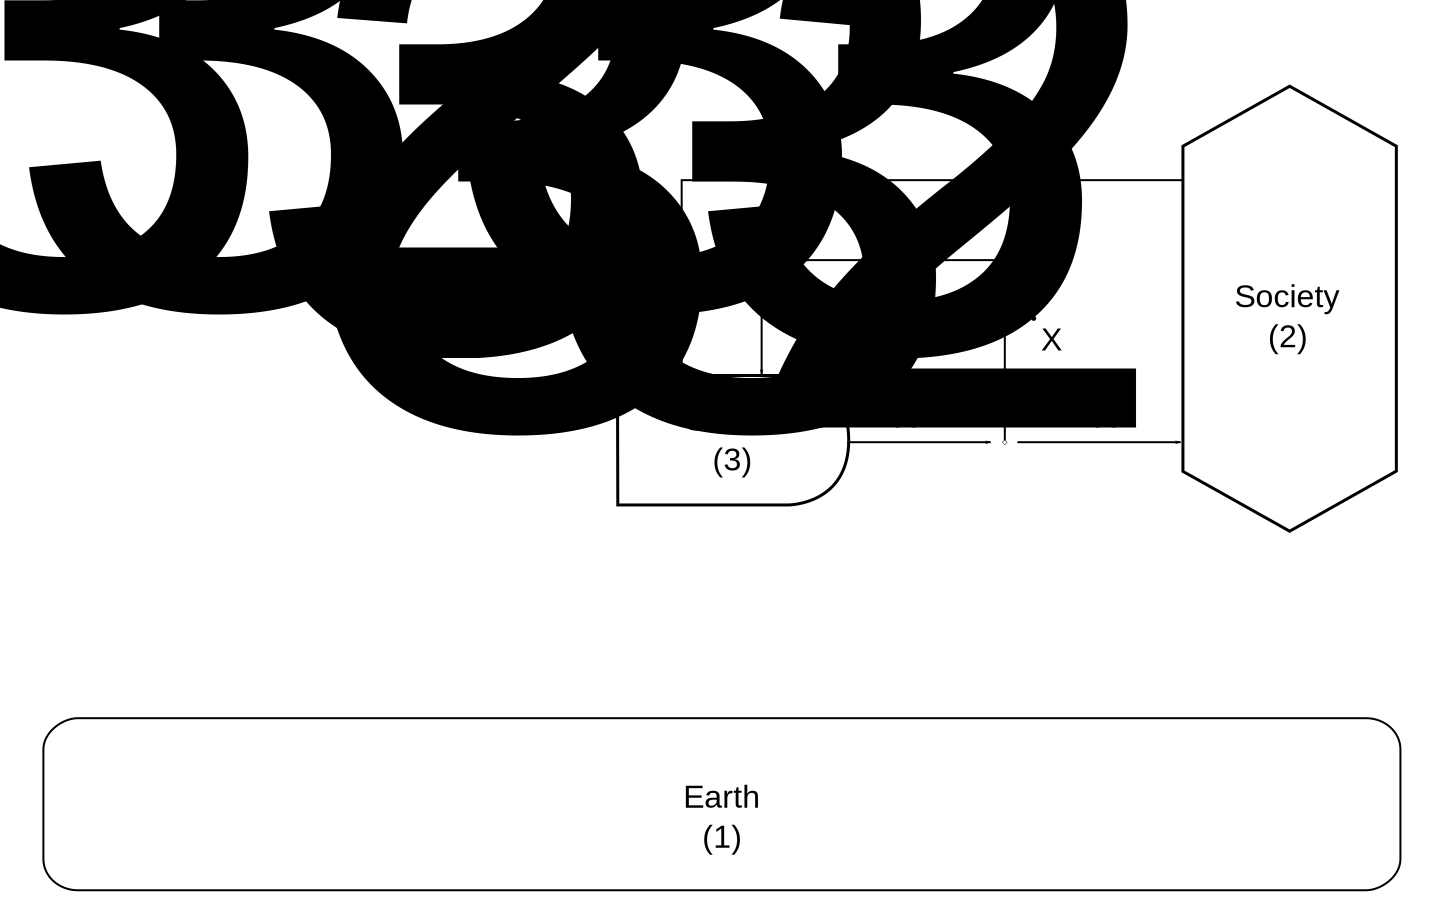
\includegraphics[width=0.8\linewidth]{Part_2/Chapter_Values/images/2_sector_value.pdf}
\caption[Flows of value within a two-sector economy.]{Flows of value ($\dot{X}$) within a two-sector economy.}
\label{fig:B_value}
\end{figure}

We can account for value flows by writing
the following equations:

\begin{equation}\label{eq:B-value-1}
	\frac{\mathrm{d}X_{1}}{\mathrm{d}t}
	= \dot{X}_{11}
	+ \dot{X}_{21}
	- \dot{X}_{1}
	+ \dot{X}_{gen,1}
	- \dot{X}_{dest,1}
\end{equation}

\noindent{}and

\begin{equation}\label{eq:B-value-2}
	\frac{\mathrm{d}X_{2}}{\mathrm{d}t}
	= \dot{X}_{12}
	+ \dot{X}_{22}
	- \dot{X}_{2}
	+ \dot{X}_{gen,2}
	- \dot{X}_{dest,2}.
\end{equation}

Equations~\ref{eq:B-value-1} and~\ref{eq:B-value-2}
can be generalized as

\begin{equation}\label{eq:B-value-generalized}
	\frac{\mathrm{d}X_{j}}{\mathrm{d}t}
	= \sum\limits_{i=1}^n \dot{X}_{ij}
	- \dot{X}_{j}
	+ \dot{X}_{gen,j}
	- \dot{X}_{dest,j},
\end{equation}

\noindent{}where $n$ is the number of sectors in the economy, and $j \in [1, n]$.


%%%%%%%%%% Example C: three-sector economy %%%%%%%%%%
\section{Example C: three-sector economy} % chktex 13
%%%%%%%%%%

Figure~\ref{fig:C_value} shows flows of value ($\dot{X}$) 
within a three-sector economy. 

\begin{figure}[!ht]
\centering
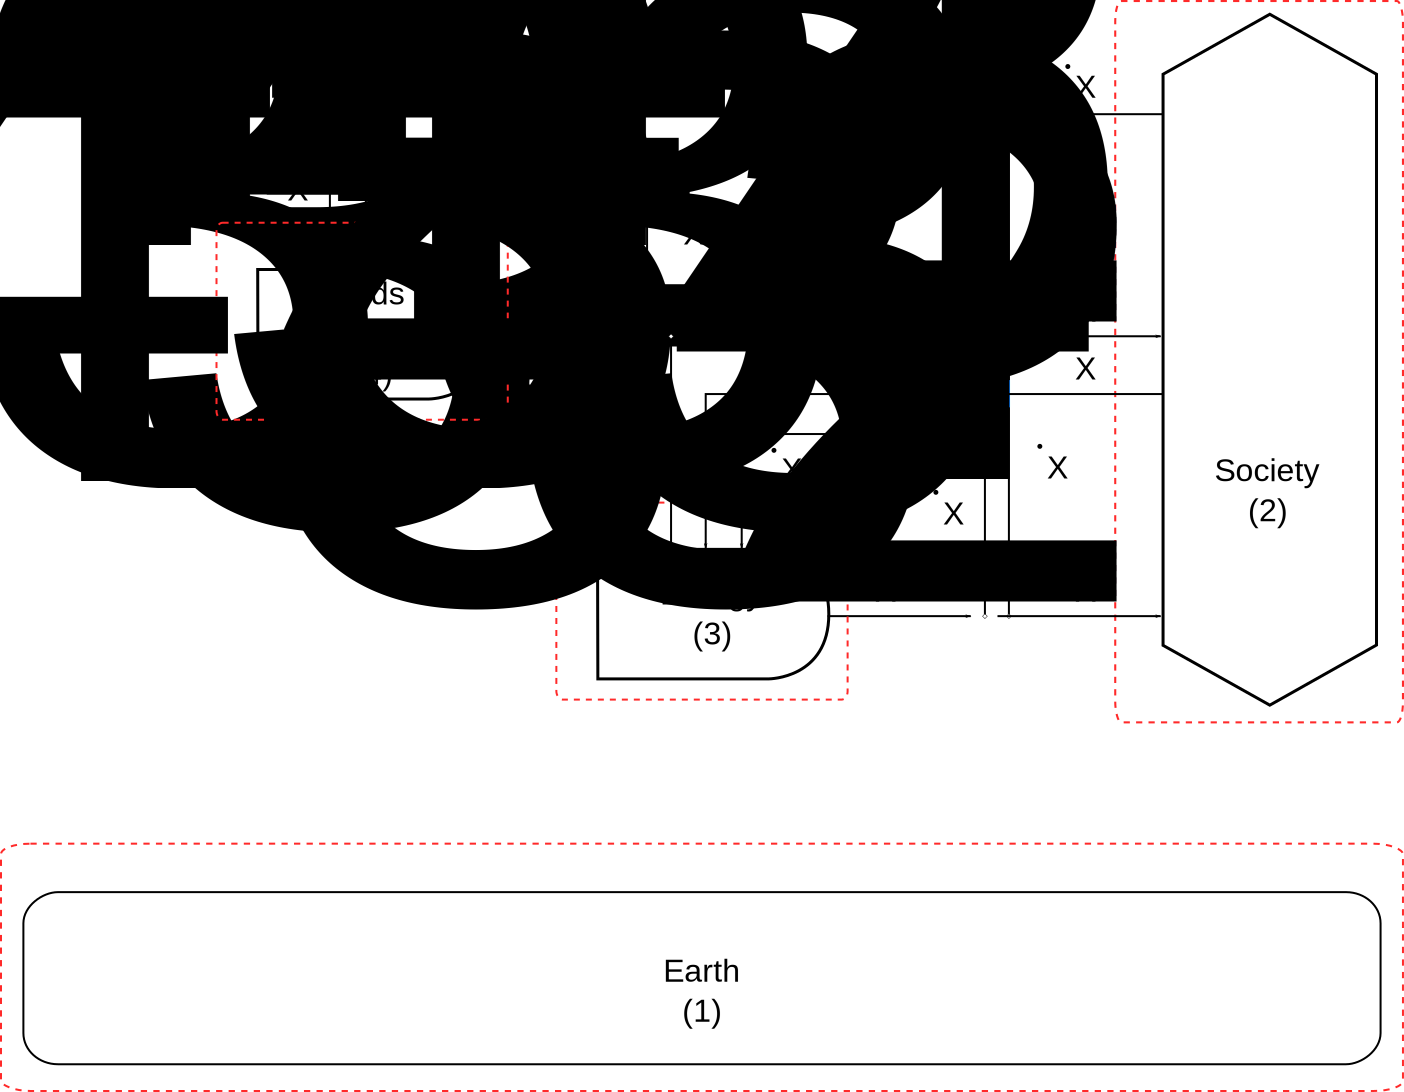
\includegraphics[width=0.8\linewidth]{Part_2/Chapter_Values/images/3_sector_value.pdf}
\caption[Flows of value within a three-sector economy.]{Flows of value ($\dot{X}$) within a three-sector economy.}
\label{fig:C_value}
\end{figure}

The equations representing flows of value in Example~C are:

\begin{equation}\label{eq:C-value-generalized}
	\frac{\mathrm{d}X_{j}}{\mathrm{d}t}
	= \sum\limits_{i=1}^{n} \dot{X}_{ij}
	- \dot{X}_{j}
	+ \dot{X}_{gen,j}
	- \dot{X}_{dest,j},
\end{equation}

\noindent{}where $n$ is the number of sectors in the economy, and $j \in [1, n]$.
Equation~\ref{eq:C-value-generalized} is identical to Equation~\ref{eq:B-value-generalized}.
If we sum the value accounting equations for the entire economy, 
we obtain

\begin{equation}\label{eq:C-value-economy-a}
	\sum\limits_{j=1}^{n} \frac{\mathrm{d}X_{j}}{\mathrm{d}t}
	= \sum\limits_{j=1}^{n} \sum\limits_{i=1}^{n} \dot{X}_{ij}
	- \sum\limits_{j=1}^{n} \dot{X}_{j}
	+ \sum\limits_{j=1}^{n} \dot{X}_{gen,j}
	- \sum\limits_{j=1}^{n} \dot{X}_{dest,j}.
\end{equation}

\noindent{}With the identities

\begin{equation} \label{eq:X_identity_1}
	\dot{X}_{j}  
	= \sum\limits_{k=1}^n \dot{X}_{jk}
\end{equation}

\noindent{}and

\begin{equation} \label{eq:X_identity_2}
	\sum\limits_{j=1}^n\dot{X}_{j}  
	= \sum\limits_{j=1}^n \sum\limits_{k=1}^n \dot{X}_{jk}
	= \sum\limits_{i=1}^n \sum\limits_{k=1}^n \dot{X}_{ik}
	= \sum\limits_{i=1}^n \sum\limits_{j=1}^n \dot{X}_{ij}
	= \sum\limits_{j=1}^n \sum\limits_{i=1}^n \dot{X}_{ij},
\end{equation}

\noindent{}Equation~\ref{eq:C-value-economy-a} becomes

\begin{equation}\label{eq:C-value-economy-b}
	\sum\limits_{j=1}^{n} \frac{\mathrm{d}X_{j}}{\mathrm{d}t}
	= \sum\limits_{j=1}^{n} \dot{X}_{gen,j}
	- \sum\limits_{j=1}^{n} \dot{X}_{dest,j},
\end{equation}

\noindent{}for $j \in [1, n]$, indicating that 
value generation ($\dot{X}_{gen,j}$) 
and destruction ($\dot{X}_{dest,j}$)
are the only mechanisms by which value is accumulated or lost
$\left( \frac{\mathrm{d}X_{j}}{\mathrm{d}t} \right)$
within the economy.


%%%%%%%%%% Value: Auto industry example %%%%%%%%%%
\section{Value in the auto industry}
\label{sec:value_auto}
%%%%%%%%%%
The theoretical model of energy and resource flows through an economy can be empirically estimated using US data available 
from the Bureau of Economic Analysis (BEA), published in their \emph{Survey of Current Business} journal. **** Need citation here. ****
 The two main tables of data needed to estimate dynamic value flows and capital accumulation within the economy 
are the Input-Output accounts (IO) and the Capital Flow Table (CFT). 
 The IO table tracks commodities that are made in one industry and then used in another as intermediate inputs. [put rdot and sdot if appropriate. If transactions include capital flows, then also include kdot.]
The “making” industries related to extraction, refining, and utilities 
mark the entry point for materials extracted from the biosphere into the economy. 
 These three industries (extraction, refining, and utilities) are the first three industries listed in the NAICS (North American Industry Classification System)
 that the BEA uses to track economic information. 
****BRH  add cite (Lawson and et al. 2002, 25). **** 

Using these data, Figure~\ref{fig:PERKS_value_auto_ind} provides estimates 
of value flows for the US auto industry.

\begin{figure}[!ht]
\centering
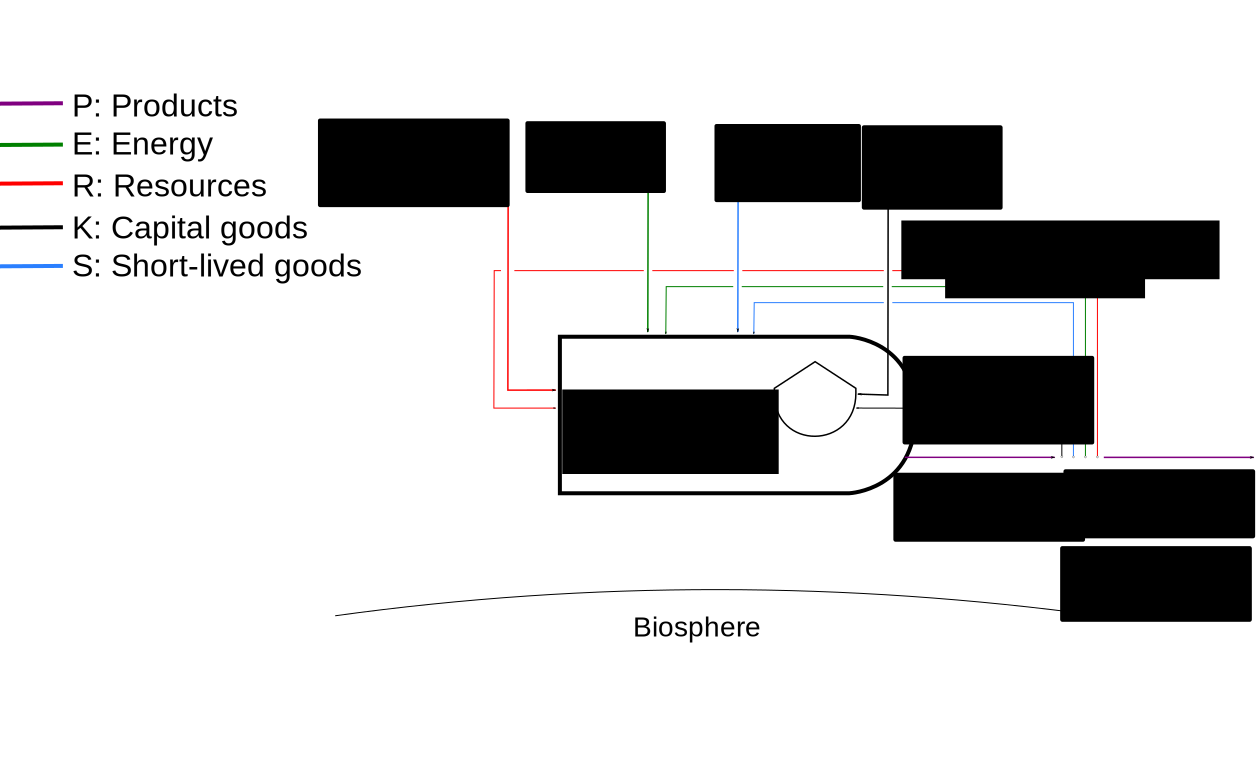
\includegraphics[width=1.0\linewidth]{Part_2/Chapter_Values/images/PERKS_basic_unit_value_auto_ind.pdf}
\caption[Value of material and energy flows into and out of the US automobile industry]{Value of material and energy flows into and out of the US automobile industry (in millions of 2011USD).}
\label{fig:PERKS_value_auto_ind}
\end{figure}

The value of capital investment, “K” in the model is measured  by the ``Capital Flow Table.'' 
This maps the outputs of construction and certain manufacturing industries to all other industries.
****BRH add cite (Bonds and Aylor 1998)****  The ``waste output to the environment''
can be approximated by the value of the commodities that are ``made'' in all industries 
and ``used'' by the ``Waste Management Sector'' (NAICS 56). 
[put \$0 instead of 441---there is a lot, but not all, of waste that 
is routed through the waste industry on its way to the biosphere.]
Using the automotive industry as an example, the KLEM **** define BRH ****S, Input-Output, 
and Capital Flow data could be used to estimate the model as demonstrated in Table~\ref{tab:data}.\footnote{See Appendix~\ref{chap:auto_value_flows} for detailed calculations.}


\begin{table}
\caption[Data Sources for Auto Industry (IOC 3361MV) Example]{Data Sources for Auto Industry (IOC 3361MV) Example.}
\begin{center}
  \begin{tabular}{l r @{\hspace{2em}} l}
   \toprule 
     & 2011 USD &   \\ 
Value Flow & (millions) & Data Source \\
	\midrule
    Resources (other than Energy) & \$207,623            & KLEMS Intermediate Use Estimates 2011 \\
&&\\
    Resources (Energy) &   3,367&   KLEMS Intermediate Use Estimates 2011                \\
&&\\
    Short-lived Goods &   42,005 &   KLEMS Intermediate Use Estimates 2011    \\
    Resources \cr (to/from Auto Industry) &  139,259 &  KLEMS Intermediate Use Estimates 2011     \\
&&\\
    Output to Waste Sector & 441  &  KLEMS Intermediate Use Estimates 2011     \\
&&\\
    Capital &  26,474  &  1997 Capital Flow Table     \\  
&&\\
    Capital (to/from Auto Industry) &  551 & 1997 Capital Flow Table      \\
&&\\
    Gross Economic Output & 467,941  &  The Use of Commodities by Industries \\
&& 1997 Capital Flow Table  \\ 
&&\\
    Net Economic Output & 327,580   &  The Use of Commodities by Industries \\
    \bottomrule
  \end{tabular}

\end{center}
\label{tab:data}
\end{table}

Thus, in contrast to the lack of data for material and energy resource flows through the economy, \emph{dollar values} of material and energy resource flows through the economy are publicly available from the BEA website. 


%%%%%%%%%% Value: Summary %%%%%%%%%%
\section{Summary}
\label{sec:value_summary}
%%%%%%%%%%

\bibliographystyle{unsrt}
\bibliography{../../EROI_review_v2}



% Always give a unique label
% and use \ref{<label>} for cross-references
% and \cite{<label>} for bibliographic references
% use \sectionmark{}
% to alter or adjust the section heading in the running head
%% Instead of simply listing headings of different levels we recommend to let every heading be followed by at least a short passage of text. Furtheron please use the \LaTeX\ automatism for all your cross-references and citations.

%% Please note that the first line of text that follows a heading is not indented, whereas the first lines of all sequent paragraphs are.

%% Use the standard \verb|equation| environment to typeset your equations, e.g.
%
%% \begin{equation}
%% a \times b = c\;,
%% \end{equation}
%
%% however, for multiline equations we recommend to use the \verb|eqnarray|
%% environment\footnote{In physics texts please activate the class option \texttt{vecphys} to depict your vectors in \textbf{\itshape boldface-italic} type - as is customary for a wide range of physical jects.}.
%% \begin{eqnarray}
%% a \times b = c \nonumber\\
%% \vec{a} \cdot \vec{b}=\vec{c}
%% \label{eq:01}
%% \end{eqnarray}

%% \section{section Heading}
%% \label{sec:2}
%% Instead of simply listing headings of different levels we recommend to let every heading be followed by at least a short passage of text. Furtheron please use the \LaTeX\ automatism for all your cross-references\index{cross-references} and citations\index{citations} as has already been described in Sect.~\ref{sec:2}.

%% \begin{quotation}
%% Please do not use quotation marks when quoting texts! Simply use the \verb|quotation| environment -- it will automatically render Springer's preferred layout.
%% \end{quotation}


%% \section{section Heading}
%% Instead of simply listing headings of different levels we recommend to let every heading be followed by at least a short passage of text. Furtheron please use the \LaTeX\ automatism for all your cross-references and citations as has already been described in Sect.~\ref{sec:2}, see also Fig.~\ref{fig:1}\footnote{If you copy text passages, figures, or tables from other works, you must obtain \textit{permission} from the copyright holder (usually the original publisher). Please enclose the signed permission with the manucript. The sources\index{permission to print} must be acknowledged either in the captions, as footnotes or in a separate section of the book.}

%% Please note that the first line of text that follows a heading is not indented, whereas the first lines of all sequent paragraphs are.

% For figures use
%
%% \begin{figure}[b]
%% \sidecaption
% Use the relevant command for your figure-insertion program
% to insert the figure file.
% For example, with the option graphics use
%% \includegraphics[scale=.65]{figure}
%
% If not, use
%\picplace{5cm}{2cm} % Give the correct figure height and width in cm
%
%% \caption{If the width of the figure is less than 7.8 cm use the \texttt{sidecapion} command to flush the caption on the left side of the page. If the figure is positioned at the top of the page, align the sidecaption with the top of the figure -- to achieve this you simply need to use the optional argument \texttt{[t]} with the \texttt{sidecaption} command}
%% \label{fig:1}       % Give a unique label
%% \end{figure}


%% \paragraph{Paragraph Heading} %
%% Instead of simply listing headings of different levels we recommend to let every heading be followed by at least a short passage of text. Furtheron please use the \LaTeX\ automatism for all your cross-references and citations as has already been described in Sect.~\ref{sec:2}.

%% Please note that the first line of text that follows a heading is not indented, whereas the first lines of all sequent paragraphs are.

%% For typesetting numbered lists we recommend to use the \verb|enumerate| environment -- it will automatically render Springer's preferred layout.

%% \begin{enumerate}
%% \item{Livelihood and survival mobility are oftentimes coutcomes of uneven socioeconomic development.}
%% \begin{enumerate}
%% \item{Livelihood and survival mobility are oftentimes coutcomes of uneven socioeconomic development.}
%% \item{Livelihood and survival mobility are oftentimes coutcomes of uneven socioeconomic development.}
%% \end{enumerate}
%% \item{Livelihood and survival mobility are oftentimes coutcomes of uneven socioeconomic development.}
%% \end{enumerate}


%% \paragraph{paragraph Heading} In order to avoid simply listing headings of different levels we recommend to let every heading be followed by at least a short passage of text. Use the \LaTeX\ automatism for all your cross-references and citations as has already been described in Sect.~\ref{sec:2}, see also Fig.~\ref{fig:2}.

%% Please note that the first line of text that follows a heading is not indented, whereas the first lines of all sequent paragraphs are.

%% For unnumbered list we recommend to use the \verb|itemize| environment -- it will automatically render Springer's preferred layout.

%% \begin{itemize}
%% \item{Livelihood and survival mobility are oftentimes coutcomes of uneven socioeconomic development, cf. Table~\ref{tab:1}.}
%% \begin{itemize}
%% \item{Livelihood and survival mobility are oftentimes coutcomes of uneven socioeconomic development.}
%% \item{Livelihood and survival mobility are oftentimes coutcomes of uneven socioeconomic development.}
%% \end{itemize}
%% \item{Livelihood and survival mobility are oftentimes coutcomes of uneven socioeconomic development.}
%% \end{itemize}

%% \begin{figure}[t]
%% \sidecaption[t]
% Use the relevant command for your figure-insertion program
% to insert the figure file.
% For example, with the option graphics use
%% \includegraphics[scale=.65]{figure}
%
% If not, use
%\picplace{5cm}{2cm} % Give the correct figure height and width in cm
%
%% \caption{Please write your figure caption here}
%% \label{fig:2}       % Give a unique label
%% \end{figure}

%% \runinhead{Run-in Heading Boldface Version} Use the \LaTeX\ automatism for all your cross-references and citations as has already been described in Sect.~\ref{sec:2}.

%% \runinhead{Run-in Heading Italic Version} Use the \LaTeX\ automatism for all your cross-refer\-ences and citations as has already been described in Sect.~\ref{sec:2}\index{paragraph}.
% Use the \index{} command to code your index words
%
% For tables use
%
%% \begin{table}
%% \caption{Please write your table caption here}
%% \label{tab:1}       % Give a unique label
%
% For LaTeX tables use
%
%% \begin{tabular}{p{2cm}p{2.4cm}p{2cm}p{4.9cm}}
%% \hline\noalign{\smallskip}
%% Classes & class & Length & Action Mechanism  \\
%% \noalign{\smallskip}\svhline\noalign{\smallskip}
%% Translation & mRNA$^a$  & 22 (19--25) & Translation repression, mRNA cleavage\\
%% Translation & mRNA cleavage & 21 & mRNA cleavage\\
%% Translation & mRNA  & 21--22 & mRNA cleavage\\
%%Translation & mRNA  & 24--26 & Histone and DNA Modification\\
%%\noalign{\smallskip}\hline\noalign{\smallskip}
%%\end{tabular}
%%$^a$ Table foot note (with superscript)
%%\end{table}
%
%% \section{Section Heading}
%%\label{sec:3}
% Always give a unique label
% and use \ref{<label>} for cross-references
% and \cite{<label>} for bibliographic references
% use \sectionmark{}
% to alter or adjust the section heading in the running head
%% Instead of simply listing headings of different levels we recommend to let every heading be followed by at least a short passage of text. Furtheron please use the \LaTeX\ automatism for all your cross-references and citations as has already been described in Sect.~\ref{sec:2}.

%% Please note that the first line of text that follows a heading is not indented, whereas the first lines of all sequent paragraphs are.

%%If you want to list definitions or the like we recommend to use the Springer-enhanced \verb|description| environment -- it will automatically render Springer's preferred layout.

%%\begin{description}[Type 1]
%%\item[Type 1]{That addresses central themes pertainng to migration, health, and disease. In Sect.~\ref{sec:1}, Wilson discusses the role of human migration in infectious disease distributions and patterns.}
%%\item[Type 2]{That addresses central themes pertainng to migration, health, and disease. In Sect.~\ref{sec:2}, Wilson discusses the role of human migration in infectious disease distributions and patterns.}
%%\end{description}

%%\section{section Heading} %
%% In order to avoid simply listing headings of different levels we recommend to let every heading be followed by at least a short passage of text. Use the \LaTeX\ automatism for all your cross-references and citations citations as has already been described in Sect.~\ref{sec:2}.

%% Please note that the first line of text that follows a heading is not indented, whereas the first lines of all sequent paragraphs are.

%% \begin{svgraybox}
%% If you want to emphasize complete paragraphs of texts we recommend to use the newly defined Springer class option \verb|graybox| and the newly defined environment \verb|svgraybox|. This will produce a 15 percent screened box 'behind' your text.

%% If you want to emphasize complete paragraphs of texts we recommend to use the newly defined Springer class option and environment \verb|svgraybox|. This will produce a 15 percent screened box 'behind' your text.
%% \end{svgraybox}


%% \section{section Heading}
%%Instead of simply listing headings of different levels we recommend to let every heading be followed by at least a short passage of text. Furtheron please use the \LaTeX\ automatism for all your cross-references and citations as has already been described in Sect.~\ref{sec:2}.

%% Please note that the first line of text that follows a heading is not indented, whereas the first lines of all sequent paragraphs are.

%% \begin{theorem}
%% Theorem text goes here.
%% \end{theorem}
%
% or
%
%% \begin{definition}
%% Definition text goes here.
%% \end{definition}

%% \begin{proof}
%\smartqed
%% Proof text goes here.
%% \qed
%% \end{proof}

%%\paragraph{Paragraph Heading} %
%% Instead of simply listing headings of different levels we recommend to let every heading be followed by at least a short passage of text. Furtheron please use the \LaTeX\ automatism for all your cross-references and citations as has already been described in Sect.~\ref{sec:2}.

%% Note that the first line of text that follows a heading is not indented, whereas the first lines of all subsequent paragraphs are.
%
% For built-in environments use
%
%%\begin{theorem}
%%Theorem text goes here.
%%\end{theorem}
%
%%\begin{definition}
%%Definition text goes here.
%%\end{definition}
%
%%\begin{proof}
%%\smartqed
%% Proof text goes here.
%%\qed
%%\end{proof}
%
%% \begin{acknowledgement}
%% If you want to include acknowledgments of assistance and the like at the end of an individual chapter please use the \verb|acknowledgement| environment -- it will automatically render Springer's preferred layout.
%% \end{acknowledgement}
%
%% \section*{Appendix}
%% \addcontentsline{toc}{section}{Appendix}
%
%% When placed at the end of a chapter or contribution (as opposed to at the end of the book), the numbering of tables, figures, and equations in the appendix section continues on from that in the main text. Hence please \textit{do not} use the \verb|appendix| command when writing an appendix at the end of your chapter or contribution. If there is only one the appendix is designated ``Appendix'', or ``Appendix 1'', or ``Appendix 2'', etc. if there is more than one.

%% \begin{equation}
%% a \times b = c
%% \end{equation}
% Problems or Exercises should be sorted chapterwise
%% \section*{Problems}
%% \addcontentsline{toc}{section}{Problems}
%
% Use the following environment.
% Don't forget to label each problem;
% the label is needed for the solutions' environment
%% \begin{prob}
%% \label{prob1}
%% A given problem or Excercise is described here. The
%% problem is described here. The problem is described here.
%% \end{prob}

%% \begin{prob}
%% \label{prob2}
%% \textbf{Problem Heading}\\
%% (a) The first part of the problem is described here.\\
%% (b) The second part of the problem is described here.
%% \end{prob}


 

%!TEX root = ../../Heun_Dale_Haney_A_dynamic_approach_to_input_output_modeling.tex
%%%%%%%%%%%%%%%%%%%%% chapter.tex %%%%%%%%%%%%%%%%%%%%%%%%%%%%%%%%%
%
% sample chapter
%
% Use this file as a template for your own input.
%
%%%%%%%%%%%%%%%%%%%%%%%% Springer-Verlag %%%%%%%%%%%%%%%%%%%%%%%%%%
%\motto{Use the template \emph{chapter.tex} to style the various elements of your chapter content.}

%%%%%%%%%%%%%%%%%%%%%%%%%%%%%%%%%%%%%%
%%%%%%%%%% Energy Intensity %%%%%%%%%%
%%%%%%%%%%%%%%%%%%%%%%%%%%%%%%%&&&&%%%
\chapter{Energy intensity}
% Always give a unique label
\label{chap:intensity} 
% use \chaptermark{} to alter or adjust the chapter heading in the running head
\chaptermark{intensity}
%%%%%%%%%%%%%%%%%%%%%%%%%%%%%%%%%%
%%%%%%%%%%%%%%%%%%%%%%%%%%%%%%%%%%
%%%%%%%%%%%%%%%%%%%%%%%%%%%%%%%%%%

\abstract*{[NEED TO ADD ABSTRACT HERE]}

%% \abstract{Each chapter should be preceded by an abstract (10--15 lines long) that summarizes the content. The abstract will appear \textit{online} at \url{www.SpringerLink.com} and be available with unrestricted access. This allows unregistered users to read the abstract as a teaser for the complete chapter. As a general rule the abstracts will not appear in the printed version of your book unless it is the style of your particular book or that of the series to which your book belongs.\newline\indent
%% Please use the 'starred' version of the new Springer \texttt{abstract} command for typesetting the text of the online abstracts (cf. source file of this chapter template \texttt{abstract}) and include them with the source files of your manuscript. Use the plain \texttt{abstract} command if the abstract is also to appear in the printed version of the book.}

%% Use the template \emph{chapter.tex} together with the Springer document class SVMono (monograph-type books) or SVMult (edited books) to style the various elements of your chapter content in the Springer layout.


In Chapters~\ref{chap:direct_energy},~\ref{chap:embodied_energy}, and~\ref{chap:value}, 
we defined flows of direct energy, embodied energy, and value in an economy.
In this chapter, we merge energy and value together to estimate
the energy intensity of economic sectors.


%%%%%%%%%% Methodology %%%%%%%%%%
\section{Methodology}
%%%%%%%%%%

Energy intensity ($\varepsilon$) is the ratio 
of total energy ($\dot{T}$) and value ($\dot{X}$) outflow rates 
from an economic sector, 
such that for the $j^{\mathrm{th}}$ goods and services sector,

\begin{equation} \label{eq:epsilon_output_def_g_and_s}
	\varepsilon_{j} \equiv \frac{\dot{T}_{j}}{\dot{X}_{j}},
\end{equation} \nomenclature[e]{$\varepsilon$}{energy intensity, J/\$}

****** Add more nomenclature from this Chapter *********

\noindent{}and $\varepsilon$ is in units of J/\$. 
For inter-sector flows, we have

\begin{equation} \label{eq:epsilon_transfers_1}
	\varepsilon_{jk} = \frac{\dot{T}_{jk}}{\dot{X}_{jk}}.
\end{equation}

Furthermore, we note that 

\begin{equation} \label{eq:epsilon_equiv_1}
	\varepsilon_{j} = \varepsilon_{jk}
\end{equation}

\noindent{}for all $k$, because the energy intensity 
of sector $j$'s output is independent of its destination ($k$). 
I.e., we assume that all goods produced by a sector 
are produced at the average energy intensity 
of that sector.\footnote{If this approach is unsatisfactory, 
the sector may be divided into sub-sectors 
with different energy intensities.}

We define the input-ouput ratio ($a_{ij}$) that represents the input 
of good $i$ required to produce a unit of output from sector $j$.

\begin{equation} \label{eq:aij_def}
	a_{ij} \equiv \frac{\dot{X}_{ij}}{\dot{X}_{j}}
\end{equation}

Input-output ratios are given in mixed units, 
depending on both the purpose of each sector of the economy 
and the type of input as shown in Figure~\ref{fig:A_matrix_units}.

\begin{figure}[h!]
\centering\
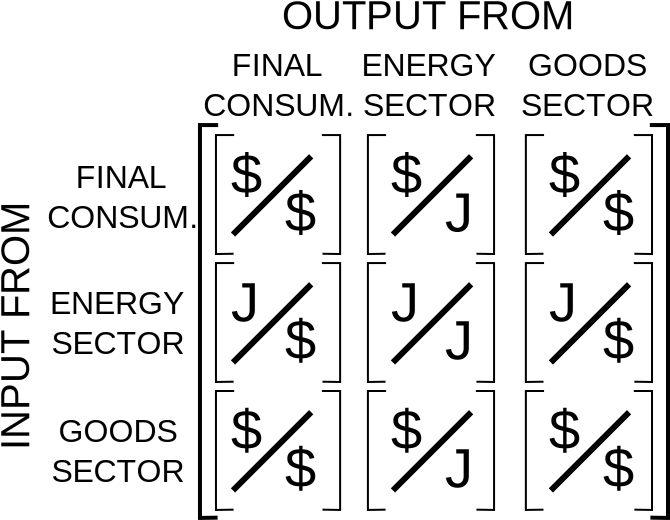
\includegraphics[width=0.4\linewidth]{Part_2/Chapter_Intensity/images/I-O_units.pdf}
\caption{Units for input-output ratios ($a$). **** Mik: Can we turn this
into a matrix where row zero and column zero represent society, 
row and column 1 represents energy, and the rest represent goods and services? ****}
\label{fig:A_matrix_units}
\end{figure}


%%%%%%%%%% Example A %%%%%%%%%%
\section{Example A: single-sector economy} % chktex 13
%%%%%%%%%%

With reference to Figures~\ref{fig:A_energy}, 
\ref{fig:A_total_energy_T_dot}, 
and~\ref{fig:A_value},
the energy intensity ($\varepsilon_{1}$) of a single-sector economy is calculated by

\begin{equation} \label{eq:A-energy_intensity}
	\varepsilon_{1} 
	= \frac{\dot{T}_{1}}{\dot{X}_{1}} 
	= \frac{\dot{T}_{11}}{\dot{X}_{11}}.
\end{equation}

Appendix~\ref{chap:infinite_series} illustrates that the energy 
intensity of a single-sector economy ($\varepsilon_{1}$) 
is comprised of the sum of the infinite recursions
of energy consumed during production of output ($\dot{X}_{1}$).

To estimate energy intensities
when more than one economic sector is involved, 
we move to Examples~B and~C in the following sections.


%%%%%%%%%% Example B %%%%%%%%%%
\section{Example B: two-sector economy} % chktex 13
%%%%%%%%%%

With reference to Figures~\ref{fig:B_energy}, 
\ref{fig:B_total_energy},
and~\ref{fig:B_value}, 
the energy intensity ($\varepsilon_{2}$) 
of the production sector is given by

\begin{equation} \label{eq:single_sector_energy_intensity}
	\varepsilon_{2} 
	= \frac{\dot{T}_{2}}{\dot{X}_{2}} 
	= \frac{\dot{T}_{22}}{\dot{X}_{22}}.
\end{equation}

\noindent{}Thus,

\begin{equation} \label{eq:T_dot_1_single_sector}
	\dot{T}_{2} = \varepsilon_{2}\dot{X}_{2},
\end{equation}

The input-output ratio 
for the production sector's self-use of output ($a_{22}$) is

\begin{equation} \label{eq:io_ratio_single_sector}
	a_{22} = \frac{\dot{X}_{22}}{\dot{X}_{2}},
\end{equation}

\noindent{}thus

\begin{equation} \label{eq:T_dot_11_single_sector}
	\dot{T}_{22} = \varepsilon_{2}a_{22}\dot{X}_{2}.
\end{equation}

Realizing that 
(a) $\frac{\mathrm{d}T_2}{\mathrm{d}t} = \frac{\mathrm{d}B_2}{\mathrm{d}t}$ 
due to $\frac{\mathrm{d}E_2}{\mathrm{d}t} = 0$, because direct energy
does not accumulate within economic sectors and
(b) $\dot{T}_{02} = \dot{E}_{02}$ due to $\dot{B}_{02} = 0$, 
because embodied energy appears only in the \emph{output} of a sector, and
substituting Equations~\ref{eq:T_dot_1_single_sector} 
and~\ref{eq:T_dot_11_single_sector} into Equation~\ref{eq:CV_T_2} gives

\begin{equation} \label{eq:dB1/dt_single_sector_after_substituting_eps_and_a}
	\frac{\mathrm{d}B_{2}}{\mathrm{d}t} 
	= \dot{E}_{02} 
	+ \dot{T}_{12}
	+ \varepsilon_{2}a_{22}\dot{X}_{2} 
	- \varepsilon_{2}\dot{X}_{2} 
	- \gamma_{2}B_{2}.
\end{equation}

To extend Equation~\ref{eq:dB1/dt_single_sector_after_substituting_eps_and_a}
to a matrix formulation, we turn to Example~C.


%%%%%%%%%% Example C %%%%%%%%%%
\section{Example~C: three-sector economy} % chktex 13
\label{sec:C-intensity}
%%%%%%%%%%

The three-sector economy of Example~C affords an opportunity 
to develop a matrix version 
of the total energy accounting equation (\ref{eq:C-CV_T_123})
and to develop an equation that estimates the
energy intensity of economic sectors. 
We begin with a matrix version of the total energy accounting equation.


%+++++++++ Example C: Total energy equation ++++++++++
\subsection{Total energy accounting equation}
%+++++++++

We apply Equation~\ref{eq:C-CV_T_123} to the three-sector
economy shown in 
Figures~\ref{fig:C_energy},~\ref{fig:C_total_energy}, and~\ref{fig:C_value}
to obtain the following total energy accounting equations
for the Energy~(2) and Goods and Services~(3) sectors 
of the three-sector economy:

\begin{equation} \label{eq:C-Total_Energy_Sec_2-a}
	\frac{\mathrm{d}T_{2}}{\mathrm{d}t} 
	= \dot{T}_{02}  
	+ \dot{T}_{12}
	+ \dot{T}_{22}
	+ \dot{T}_{32}
	- \dot{T}_{2}
	- \dot{T}_{20}
\end{equation}

\noindent{}and

\begin{equation} \label{eq:C-Total_Energy_Sec_3-a}
	\frac{\mathrm{d}T_{3}}{\mathrm{d}t} 
	= \dot{T}_{03}  
	+ \dot{T}_{13}
	+ \dot{T}_{23}
	+ \dot{T}_{33}
	- \dot{T}_{3}
	- \dot{T}_{30}.
\end{equation}

\noindent{}Similar to Example~B, we realize that 
(a) $\frac{\mathrm{d}T_i}{\mathrm{d}t} = \frac{\mathrm{d}B_i}{\mathrm{d}t}$ 
due to $\frac{\mathrm{d}E_i}{\mathrm{d}t} = 0$, because direct energy
does not accumulate within economic sectors and
(b) $\dot{T}_{0j} = \dot{E}_{0j}$ due to $\dot{B}_{0j} = 0$, 
because embodied energy appears only in the \emph{output} of a sector, and
we substitute $\dot{T}_{j} = \varepsilon_{j} \dot{X}_{j}$ 
and $\dot{T}_{jk} = \varepsilon_{j} \dot{X}_{jk}$ 
into Equations~\ref{eq:C-Total_Energy_Sec_2-a}
and~\ref{eq:C-Total_Energy_Sec_3-a} to obtain

\begin{equation} \label{eq:C-Total_Energy_Sec_2-b}
	\frac{\mathrm{d}B_{2}}{\mathrm{d}t}
	= \dot{E}_{02}
	+ \dot{T}_{12}
	+ \varepsilon_{2} \dot{X}_{22}
	+ \varepsilon_{3} \dot{X}_{32}
	- \varepsilon_{2} \dot{X}_{2}
	- \gamma_{2} B_{2}
\end{equation}

\noindent{}and

\begin{equation} \label{eq:C-Total_Energy_Sec_3-b}
	\frac{\mathrm{d}B_{3}}{\mathrm{d}t}
	= \dot{E}_{03}
	+ \dot{T}_{13}
	+ \varepsilon_{2} \dot{X}_{23}
	+ \varepsilon_{3} \dot{X}_{33}
	- \varepsilon_{3} \dot{X}_{3}
	- \gamma_{3} B_{3}.
\end{equation}


%%%%%%%%%% Example C: Matrix formulation %%%%%%%%%%
\subsection{Matrix formulation} % chktex 13
\label{sec:C-matrix}
%%%%%%%%%%

\noindent{}Equations~\ref{eq:C-Total_Energy_Sec_2-b} 
and~\ref{eq:C-Total_Energy_Sec_3-b} can be rewritten 
in matrix notation as

\begin{equation} \label{eq:C-Expanded_Matrix_Form}
	\begin{split}
		\begin{Bmatrix}
			\frac{\mathrm{d}B_{2}}{\mathrm{d}t} \\[0.4em] % Adds some vertical space.
			\frac{\mathrm{d}B_{3}}{\mathrm{d}t} 
		\end{Bmatrix}
		=
		\begin{Bmatrix}
			\dot{E}_{02}\\
			\dot{E}_{03}
		\end{Bmatrix}
		& +                                               % & sets alighment tab
		\begin{Bmatrix}
			\dot{T}_{12}\\
			\dot{T}_{13}
		\end{Bmatrix}
		+
		\begin{bmatrix}
			\dot{X}_{22} & \dot{X}_{32}\\
			\dot{X}_{23} & \dot{X}_{33}
		\end{bmatrix}
		\begin{Bmatrix}
			\varepsilon_{2}\\
			\varepsilon_{3}
		\end{Bmatrix} \\                                  % \\ gives line break
		& -                                               % & aligns to previous tab
		\begin{bmatrix}
			\dot{X}_{2} & 0          \\
			0           & \dot{X}_{3}
		\end{bmatrix}
		\begin{Bmatrix}
			\varepsilon_{2}\\
			\varepsilon_{3}
		\end{Bmatrix}
		-
		\begin{bmatrix}
			\gamma_{2} & 0          \\
			0          & \gamma_{3}
		\end{bmatrix}
		\begin{Bmatrix}
			B_{2}\\
			B_{3}
		\end{Bmatrix}		
	\end{split}
\end{equation}

\noindent{}If we define the following matrices and vectors:

\begin{equation} \label{eq:dBdt_vec_def}
	\frac{\mathrm{d}\vec{B}}{\mathrm{d}t} 
	\equiv
	\begin{Bmatrix}	
		\frac{\mathrm{d}B_{2}}{\mathrm{d}t}	\\[0.4em] % Adds some vertical space.
		\frac{\mathrm{d}B_{3}}{\mathrm{d}t}
	\end{Bmatrix},
\end{equation}

\begin{equation} \label{eq:E_vec_def}
	\vec{E}_{0} 
	\equiv
	\begin{Bmatrix}
		\dot{E}_{02} \\
		\dot{E}_{03}
	\end{Bmatrix},
\end{equation}

\begin{equation} \label{eq:T_vec_def}
	\vec{T}_{1} 
	\equiv
	\begin{Bmatrix}
		\dot{T}_{12} \\
		\dot{T}_{13}
	\end{Bmatrix},
\end{equation}

\begin{equation} \label{eq:X_t_matrix_def}
	\vec{X}_{t} 
	\equiv
	\begin{bmatrix}
		\dot{X}_{22} & \dot{X}_{23} \\
		\dot{X}_{32} & \dot{X}_{33}
	\end{bmatrix},
\end{equation}

\begin{equation} \label{eq:eps_vec_def}
	\bm{\varepsilon} 
	\equiv
	\begin{Bmatrix}
		\varepsilon_{2}	\\
		\varepsilon_{3}
	\end{Bmatrix},
\end{equation}

\begin{equation} \label{eq:X_hat_matrix_def}
	\hat{\vec{X}} 
	\equiv
	\delta_{ij} \dot{X}_{j} 
	= 
	\begin{bmatrix}
		\dot{X}_{2}		&	0	  \\
		0				&	\dot{X}_{3}	\\
	\end{bmatrix},
\end{equation}

\begin{equation} \label{eq:gamma_hat_matrix_def}
	\hat{\bm{\gamma}}
	\equiv
	\delta_{ij} \gamma_{j}
	=
	\begin{bmatrix}
		\gamma_{2} & 0         \\
		0          & \gamma_{3}
	\end{bmatrix},
\end{equation}

\noindent{}and

\begin{equation} \label{eq:B_vec_def}
	\vec{B} 
	\equiv
	\begin{Bmatrix}	
		B_{2} \\
		B_{3}
	\end{Bmatrix};
\end{equation}

\noindent{}with the ``Kronecker delta''

\begin{equation}\label{eq:k_delta}
	\delta_{ij} 
	=
	\begin{cases}	
		0	&	\text{if  } i \neq j	\\
		1 	& 	\text{if  } i = j
	\end{cases};
\end{equation}

\noindent{}we can rewrite Equation~\ref{eq:C-Expanded_Matrix_Form}
compactly as

\begin{equation} \label{eq:matrix_leontief_pre_1}
	\frac{\mathrm{d}\vec{B}}{\mathrm{d}t} 
	= \vec{E}_{0}
	+ \vec{T}_{1}
	+ \vec{X}_{t}^{\mathrm{T}}\bm{\varepsilon} 
	- \hat{\vec{X}}\bm{\varepsilon}
	- \hat{\bm{\gamma}}\vec{B}.
\end{equation}

\noindent{}Equation~\ref{eq:matrix_leontief_pre_1} can be simplified to

\begin{equation} \label{eq:matrix_leontief_pre_2}
	\frac{\mathrm{d}\vec{B}}{\mathrm{d}t} 
	= \vec{E}_{0}
	+ \vec{T}_{1}
	+ (\vec{X}_{t}^{\mathrm{T}} - \hat{\vec{X}})\bm{\varepsilon} 
	- \hat{\bm{\gamma}}\vec{B}.
\end{equation}

\noindent{}We can define the input-output matrix ($\vec{A}$) as

\begin{equation} \label{eq:A_matrix_def}
	\vec{A} 
	\equiv
	\begin{bmatrix}
		a_{22} & a_{23}	\\
		a_{32} & a_{33}	
	\end{bmatrix}.
\end{equation}

\noindent{}Appendix~\ref{app:Proof} shows that

\begin{equation} \label{eq:Xdifference1}
	\vec{X}_{t}^{\mathrm{T}} 
	- \hat{\vec{X}} 
	= \hat{\vec{X}} (\vec{A}^{\mathrm{T}} - \vec{I}),
\end{equation}

\noindent{}which allows Equation~\ref{eq:matrix_leontief_pre_2}
to be recast as

\begin{equation} \label{eq:matrix_leontief}
	\frac{\mathrm{d}\vec{B}}{\mathrm{d}t} 
	= \vec{E}_{0}
	+ \vec{T}_{1}
	+ \hat{\vec{X}} (\vec{A}^{\mathrm{T}} - \vec{I})\bm{\varepsilon} 
	- \hat{\bm{\gamma}}\vec{B}.
\end{equation}

\noindent{}Equation~\ref{eq:matrix_leontief} is the matrix version 
of the total energy accounting equation
written in terms of energy intensities ($\bm{\varepsilon}$)
and input-output ratios ($\vec{A}$).
Equation~\ref{eq:C-Expanded_Matrix_Form} applies 
for the three-sector economy of Example~C, 
but the equivalent matrix formulation (Equation~\ref{eq:matrix_leontief}) 
can be extended to any desired level 
of economic and energy sector disaggregation 
by expanding the vectors and matrices in 
Equations~\ref{eq:dBdt_vec_def}--\ref{eq:B_vec_def}
and~\ref{eq:A_matrix_def} to include
all sectors of the economy.\cite{Casler1984,Bullard:1978vd}

Equation~\ref{eq:matrix_leontief} provides a means to 
estimate the embodied energy accumulation rate
in economic sectors $\left(\frac{\mathrm{d}\vec{B}}{\mathrm{d}t}\right)$ 
knowing only 
direct energy inputs to the economy from the biosphere ($\vec{E}_{0}$), 
total energy inputs from society to the economy ($\vec{T}_{1}$),
sector outputs ($\hat{\vec{X}}$), 
sector input-output ratios ($\vec{A}$), 
sector energy intensities ($\bm{\varepsilon}$), 
and sector physical depreciation rates ($\hat{\bm{\gamma}}\vec{B}$). 
In theory, the transaction matrix ($\vec{X}_{t}$) is not required 
if the input-ouput matrix ($\vec{A}$) is known, 
though in practice, 
knowledge of input-output matrix ($\vec{A}$) 
would be derived from the transaction matrix ($\vec{X}_{t}$),
as shown by Equation~\ref{eq:Xdifference1Proof-9}.


%%%%%%%%%% Example C %%%%%%%%%%
\section{Estimating $\bm{\varepsilon}$}
%%%%%%%%%%

Equation~\ref{eq:matrix_leontief} can be rearranged to obtain

\begin{equation} \label{eq:epsilon_derivation_1}
	\hat{\vec{X}} (\vec{A}^{\mathrm{T}} - \vec{I}) \bm{\epsilon}
	= \frac{\mathrm{d}\vec{B}}{\mathrm{d}t}
	+ \hat{\bm{\gamma}} \vec{B}
	- \vec{E}_{0}
	- \vec{T}_{1} 
\end{equation}

\noindent{}and

\begin{equation} \label{eq:epsilon_derivation_2}
	\bm{\epsilon}
	= {\left[ \hat{\vec{X}} (\vec{A}^{\mathrm{T}} - \vec{I}) \right]}^{-1}
		\left[
			\frac{\mathrm{d}\vec{B}}{\mathrm{d}t}
			+ \hat{\bm{\gamma}} \vec{B}
			- \vec{E}_{0}
			- \vec{T}_{1} 
		\right].
\end{equation}

\noindent{}We apply the matrix identity~\cite[Formula 6.2, p. 308]{Beyer:1991vd}

\begin{equation} \label{eq:matrix_identity_Beyer}
	{\left(\vec{A}\vec{B}\vec{C}\right)}^{-1} 
	= \vec{C}^{-1} \vec{B}^{-1} \vec{A}^{-1}
\end{equation}

\noindent{}to the right side of Equation~\ref{eq:epsilon_derivation_2} to obtain

\begin{equation} \label{eq:epsilon_derivation_3}
	\bm{\epsilon}
	= {(\vec{A}^{\mathrm{T}} - \vec{I})}^{-1} {\hat{\vec{X}}}^{-1} 
		\left[
			\frac{\mathrm{d}\vec{B}}{\mathrm{d}t}
			+ \hat{\bm{\gamma}} \vec{B}
			- \vec{E}_{0}
			- \vec{T}_{1} 
		\right].
\end{equation}

\noindent{}Changing signs on the right side 
of Equation~\ref{eq:epsilon_derivation_2} gives

\begin{equation} \label{eq:epsilon_leontief_with_A}
	\bm{\varepsilon} 
	= {(\vec{I} - \vec{A}^{\mathrm{T}})}^{-1}\hat{\vec{X}}^{-1}
		\left[\vec{E}_{0} 
				+ \vec{T}_{1} 
				- \frac{\mathrm{d}\vec{B}}{\mathrm{d}t} 
				- \hat{\bm{\gamma}}\vec{B}
		\right].
\end{equation}

\noindent{}Equation~\ref{eq:epsilon_leontief_with_A} allows estimation 
of the energy intensity 
of economic sectors ($\bm{\varepsilon}$) 
knowing only 
sector input-output ratios ($\vec{A}$), 
sector outputs ($\hat{\vec{X}}$), 
energy input to the economy from the biosphere ($\vec{E}_{0}$), 
total energy input from society to the economy ($\vec{T}_{1}$),
sector embodied energy accumulation rates $\left(\frac{\mathrm{d}\vec{B}}{\mathrm{d}t}\right)$,
and sector physical depreciation rates ($\hat{\bm{\gamma}}\vec{B}$).

Again, the transaction matrix ($\vec{X}_{t}$) is not required 
for estimating the energy intensity of economic sectors ($\bm{\varepsilon}$)
if the input-ouput matrix ($\vec{A}$) is known, 
though in practice, 
knowledge of input-output matrix ($\vec{A}$) 
would be derived from the transaction matrix ($\vec{X}_{t}$),
as shown by Equation~\ref{eq:Xdifference1Proof-9}.


%%%%%%%%%% Intensity: Auto industry example %%%%%%%%%%
\section{Energy intensity of the auto industry}
\label{sec:intensity_auto}
%%%%%%%%%%

***** Becky complete this section. Is there anything to include here? *****

%%%%%%%%%% Intensity: Summary %%%%%%%%%%
\section{Summary}
\label{sec:intensity_summary}
%%%%%%%%%%





\bibliographystyle{unsrt}
\bibliography{../../EROI_review_v2}


% Always give a unique label
% and use \ref{<label>} for cross-references
% and \cite{<label>} for bibliographic references
% use \sectionmark{}
% to alter or adjust the section heading in the running head
%% Instead of simply listing headings of different levels we recommend to let every heading be followed by at least a short passage of text. Furtheron please use the \LaTeX\ automatism for all your cross-references and citations.

%% Please note that the first line of text that follows a heading is not indented, whereas the first lines of all sequent paragraphs are.

%% Use the standard \verb|equation| environment to typeset your equations, e.g.
%
%% \begin{equation}
%% a \times b = c\;,
%% \end{equation}
%
%% however, for multiline equations we recommend to use the \verb|eqnarray|
%% environment\footnote{In physics texts please activate the class option \texttt{vecphys} to depict your vectors in \textbf{\itshape boldface-italic} type - as is customary for a wide range of physical jects.}.
%% \begin{eqnarray}
%% a \times b = c \nonumber\\
%% \vec{a} \cdot \vec{b}=\vec{c}
%% \label{eq:01}
%% \end{eqnarray}

%% \section{section Heading}
%% \label{sec:2}
%% Instead of simply listing headings of different levels we recommend to let every heading be followed by at least a short passage of text. Furtheron please use the \LaTeX\ automatism for all your cross-references\index{cross-references} and citations\index{citations} as has already been described in Sect.~\ref{sec:2}.

%% \begin{quotation}
%% Please do not use quotation marks when quoting texts! Simply use the \verb|quotation| environment -- it will automatically render Springer's preferred layout.
%% \end{quotation}


%% \section{section Heading}
%% Instead of simply listing headings of different levels we recommend to let every heading be followed by at least a short passage of text. Furtheron please use the \LaTeX\ automatism for all your cross-references and citations as has already been described in Sect.~\ref{sec:2}, see also Fig.~\ref{fig:1}\footnote{If you copy text passages, figures, or tables from other works, you must obtain \textit{permission} from the copyright holder (usually the original publisher). Please enclose the signed permission with the manucript. The sources\index{permission to print} must be acknowledged either in the captions, as footnotes or in a separate section of the book.}

%% Please note that the first line of text that follows a heading is not indented, whereas the first lines of all sequent paragraphs are.

% For figures use
%
%% \begin{figure}[b]
%% \sidecaption
% Use the relevant command for your figure-insertion program
% to insert the figure file.
% For example, with the option graphics use
%% \includegraphics[scale=.65]{figure}
%
% If not, use
%\picplace{5cm}{2cm} % Give the correct figure height and width in cm
%
%% \caption{If the width of the figure is less than 7.8 cm use the \texttt{sidecapion} command to flush the caption on the left side of the page. If the figure is positioned at the top of the page, align the sidecaption with the top of the figure -- to achieve this you simply need to use the optional argument \texttt{[t]} with the \texttt{sidecaption} command}
%% \label{fig:1}       % Give a unique label
%% \end{figure}


%% \paragraph{Paragraph Heading} %
%% Instead of simply listing headings of different levels we recommend to let every heading be followed by at least a short passage of text. Furtheron please use the \LaTeX\ automatism for all your cross-references and citations as has already been described in Sect.~\ref{sec:2}.

%% Please note that the first line of text that follows a heading is not indented, whereas the first lines of all sequent paragraphs are.

%% For typesetting numbered lists we recommend to use the \verb|enumerate| environment -- it will automatically render Springer's preferred layout.

%% \begin{enumerate}
%% \item{Livelihood and survival mobility are oftentimes coutcomes of uneven socioeconomic development.}
%% \begin{enumerate}
%% \item{Livelihood and survival mobility are oftentimes coutcomes of uneven socioeconomic development.}
%% \item{Livelihood and survival mobility are oftentimes coutcomes of uneven socioeconomic development.}
%% \end{enumerate}
%% \item{Livelihood and survival mobility are oftentimes coutcomes of uneven socioeconomic development.}
%% \end{enumerate}


%% \paragraph{paragraph Heading} In order to avoid simply listing headings of different levels we recommend to let every heading be followed by at least a short passage of text. Use the \LaTeX\ automatism for all your cross-references and citations as has already been described in Sect.~\ref{sec:2}, see also Fig.~\ref{fig:2}.

%% Please note that the first line of text that follows a heading is not indented, whereas the first lines of all sequent paragraphs are.

%% For unnumbered list we recommend to use the \verb|itemize| environment -- it will automatically render Springer's preferred layout.

%% \begin{itemize}
%% \item{Livelihood and survival mobility are oftentimes coutcomes of uneven socioeconomic development, cf. Table~\ref{tab:1}.}
%% \begin{itemize}
%% \item{Livelihood and survival mobility are oftentimes coutcomes of uneven socioeconomic development.}
%% \item{Livelihood and survival mobility are oftentimes coutcomes of uneven socioeconomic development.}
%% \end{itemize}
%% \item{Livelihood and survival mobility are oftentimes coutcomes of uneven socioeconomic development.}
%% \end{itemize}

%% \begin{figure}[t]
%% \sidecaption[t]
% Use the relevant command for your figure-insertion program
% to insert the figure file.
% For example, with the option graphics use
%% \includegraphics[scale=.65]{figure}
%
% If not, use
%\picplace{5cm}{2cm} % Give the correct figure height and width in cm
%
%% \caption{Please write your figure caption here}
%% \label{fig:2}       % Give a unique label
%% \end{figure}

%% \runinhead{Run-in Heading Boldface Version} Use the \LaTeX\ automatism for all your cross-references and citations as has already been described in Sect.~\ref{sec:2}.

%% \runinhead{Run-in Heading Italic Version} Use the \LaTeX\ automatism for all your cross-refer\-ences and citations as has already been described in Sect.~\ref{sec:2}\index{paragraph}.
% Use the \index{} command to code your index words
%
% For tables use
%
%% \begin{table}
%% \caption{Please write your table caption here}
%% \label{tab:1}       % Give a unique label
%
% For LaTeX tables use
%
%% \begin{tabular}{p{2cm}p{2.4cm}p{2cm}p{4.9cm}}
%% \hline\noalign{\smallskip}
%% Classes & class & Length & Action Mechanism  \\
%% \noalign{\smallskip}\svhline\noalign{\smallskip}
%% Translation & mRNA$^a$  & 22 (19--25) & Translation repression, mRNA cleavage\\
%% Translation & mRNA cleavage & 21 & mRNA cleavage\\
%% Translation & mRNA  & 21--22 & mRNA cleavage\\
%%Translation & mRNA  & 24--26 & Histone and DNA Modification\\
%%\noalign{\smallskip}\hline\noalign{\smallskip}
%%\end{tabular}
%%$^a$ Table foot note (with superscript)
%%\end{table}
%
%% \section{Section Heading}
%%\label{sec:3}
% Always give a unique label
% and use \ref{<label>} for cross-references
% and \cite{<label>} for bibliographic references
% use \sectionmark{}
% to alter or adjust the section heading in the running head
%% Instead of simply listing headings of different levels we recommend to let every heading be followed by at least a short passage of text. Furtheron please use the \LaTeX\ automatism for all your cross-references and citations as has already been described in Sect.~\ref{sec:2}.

%% Please note that the first line of text that follows a heading is not indented, whereas the first lines of all sequent paragraphs are.

%%If you want to list definitions or the like we recommend to use the Springer-enhanced \verb|description| environment -- it will automatically render Springer's preferred layout.

%%\begin{description}[Type 1]
%%\item[Type 1]{That addresses central themes pertainng to migration, health, and disease. In Sect.~\ref{sec:1}, Wilson discusses the role of human migration in infectious disease distributions and patterns.}
%%\item[Type 2]{That addresses central themes pertainng to migration, health, and disease. In Sect.~\ref{sec:2}, Wilson discusses the role of human migration in infectious disease distributions and patterns.}
%%\end{description}

%%\section{section Heading} %
%% In order to avoid simply listing headings of different levels we recommend to let every heading be followed by at least a short passage of text. Use the \LaTeX\ automatism for all your cross-references and citations citations as has already been described in Sect.~\ref{sec:2}.

%% Please note that the first line of text that follows a heading is not indented, whereas the first lines of all sequent paragraphs are.

%% \begin{svgraybox}
%% If you want to emphasize complete paragraphs of texts we recommend to use the newly defined Springer class option \verb|graybox| and the newly defined environment \verb|svgraybox|. This will produce a 15 percent screened box 'behind' your text.

%% If you want to emphasize complete paragraphs of texts we recommend to use the newly defined Springer class option and environment \verb|svgraybox|. This will produce a 15 percent screened box 'behind' your text.
%% \end{svgraybox}


%% \section{section Heading}
%%Instead of simply listing headings of different levels we recommend to let every heading be followed by at least a short passage of text. Furtheron please use the \LaTeX\ automatism for all your cross-references and citations as has already been described in Sect.~\ref{sec:2}.

%% Please note that the first line of text that follows a heading is not indented, whereas the first lines of all sequent paragraphs are.

%% \begin{theorem}
%% Theorem text goes here.
%% \end{theorem}
%
% or
%
%% \begin{definition}
%% Definition text goes here.
%% \end{definition}

%% \begin{proof}
%\smartqed
%% Proof text goes here.
%% \qed
%% \end{proof}

%%\paragraph{Paragraph Heading} %
%% Instead of simply listing headings of different levels we recommend to let every heading be followed by at least a short passage of text. Furtheron please use the \LaTeX\ automatism for all your cross-references and citations as has already been described in Sect.~\ref{sec:2}.

%% Note that the first line of text that follows a heading is not indented, whereas the first lines of all subsequent paragraphs are.
%
% For built-in environments use
%
%%\begin{theorem}
%%Theorem text goes here.
%%\end{theorem}
%
%%\begin{definition}
%%Definition text goes here.
%%\end{definition}
%
%%\begin{proof}
%%\smartqed
%% Proof text goes here.
%%\qed
%%\end{proof}
%
%% \begin{acknowledgement}
%% If you want to include acknowledgments of assistance and the like at the end of an individual chapter please use the \verb|acknowledgement| environment -- it will automatically render Springer's preferred layout.
%% \end{acknowledgement}
%
%% \section*{Appendix}
%% \addcontentsline{toc}{section}{Appendix}
%
%% When placed at the end of a chapter or contribution (as opposed to at the end of the book), the numbering of tables, figures, and equations in the appendix section continues on from that in the main text. Hence please \textit{do not} use the \verb|appendix| command when writing an appendix at the end of your chapter or contribution. If there is only one the appendix is designated ``Appendix'', or ``Appendix 1'', or ``Appendix 2'', etc. if there is more than one.

%% \begin{equation}
%% a \times b = c
%% \end{equation}
% Problems or Exercises should be sorted chapterwise
%% \section*{Problems}
%% \addcontentsline{toc}{section}{Problems}
%
% Use the following environment.
% Don't forget to label each problem;
% the label is needed for the solutions' environment
%% \begin{prob}
%% \label{prob1}
%% A given problem or Excercise is described here. The
%% problem is described here. The problem is described here.
%% \end{prob}

%% \begin{prob}
%% \label{prob2}
%% \textbf{Problem Heading}\\
%% (a) The first part of the problem is described here.\\
%% (b) The second part of the problem is described here.
%% \end{prob}


 

\part{Implications, Issues, and Summary}
\label{part:implications}

%!TEX root = ../../Heun_Dale_Haney_A_dynamic_approach_to_input_output_modeling.tex
%%%%%%%%%%%%%%%%%%%%% chapter.tex %%%%%%%%%%%%%%%%%%%%%%%%%%%%%%%%%
%
% sample chapter
%
% Use this file as a template for your own input.
%
%%%%%%%%%%%%%%%%%%%%%%%% Springer-Verlag %%%%%%%%%%%%%%%%%%%%%%%%%%
%\motto{Use the template \emph{chapter.tex} to style the various elements of your chapter content.}
\motto{You can't control what you don't measure. 

\hfill---\emph{business axiom}}

%%%%%%%%%%%%%%%%%%%%%%%%%%%%%%%%%%
%%%%%%%%%% Implications %%%%%%%%%%
%%%%%%%%%%%%%%%%%%%%%%%%%%%%%%%%%%
\chapter{Implications}
% Always give a unique label
\label{chap:implications}
% use \chaptermark{} to alter or adjust the chapter heading in the running head
\chaptermark{Implications}
%%%%%%%%%%%%%%%%%%%%%%%%%%%%%%%%%%
%%%%%%%%%%%%%%%%%%%%%%%%%%%%%%%%%%
%%%%%%%%%%%%%%%%%%%%%%%%%%%%%%%%%%

\abstract*{[NEED TO ADD ABSTRACT HERE]}

%% \abstract{Each chapter should be preceded by an abstract (10--15 lines long) that summarizes the content. The abstract will appear \textit{online} at \url{www.SpringerLink.com} and be available with unrestricted access. This allows unregistered users to read the abstract as a teaser for the complete chapter. As a general rule the abstracts will not appear in the printed version of your book unless it is the style of your particular book or that of the series to which your book belongs.\newline\indent
%% Please use the 'starred' version of the new Springer \texttt{abstract} command for typesetting the text of the online abstracts (cf. source file of this chapter template \texttt{abstract}) and include them with the source files of your manuscript. Use the plain \texttt{abstract} command if the abstract is also to appear in the printed version of the book.}

%% Use the template \emph{chapter.tex} together with the Springer document class SVMono (monograph-type books) or SVMult (edited books) to style the various elements of your chapter content in the Springer layout.


Several implications can be drawn from the detailed development 
of a framework for materials and energy accounting 
(in Chapters~\ref{chap:materials}--\ref{chap:intensity})
that includes energy input from society to the economy,
embodied energy accumulation, waste material flows, and depreciation.


%%%%%%%%%% Implications for the I-O method %%%%%%%%%%
\section{Implications for the I-O method}
\label{sec:Implications_for_IO}
%%%%%%%%%%

The first set of implications are for the I-O method itself;
specifically, for the process of estimating
the energy intensity of economic output ($\bm{\varepsilon}$).


%%%%%%%%%% I-O implications: estimating epsilon %%%%%%%%%%
\subsection{Estimating $\bm{\varepsilon}$}
\label{sec:estimating_epsilon-implications_chapter}
%%%%%%%%%%

Extension of the Leontief\index{Leontief} 
Input-Output method\index{input-output method}
for energy analysis has allowed energy analysts to estimate 
the energy intensity\index{energy intensity}
of economic products ($\bm{\varepsilon}$). 
As discussed in Section~\ref{sec:Value_Methodology},
we do not take this important result as a license
to declare an intrinsic ``energy theory of value.''
\index{theory of value!energy}
Rather, we belive that energy intensity is an 
important and useful metric that can assess 
the energy performance of economies,
even within the prevailing subjective theory of value
\index{theory of value!subjective}
that underlies modern economics. 
Thus, it is important to consider the assumptions behind
the literature's presentation of the I-O method 
for estimating the energy intensity economic output.

In this manuscript, Equation~\ref{eq:epsilon_leontief_with_A} 
provides a means of estimating the energy intensity of economic sectors:

\begin{equation}
	\bm{\varepsilon} 
	= {(\vec{I} - \vec{A}^{\mathrm{T}})}^{-1}\hat{\vec{X}}^{-1}
		\left[\vec{E}_{0} 
				+ \vec{T}_{1} 
				- \frac{\mathrm{d}\vec{B}_{K}}{\mathrm{d}t} 
				- \vec{B}_{waste}
				- \hat{\bm{\gamma}}_{B}\vec{B}_{K}
		\right].\tag{\ref{eq:epsilon_leontief_with_A}}
\end{equation}

\noindent{}The I-O literature~\cite{Bullard1975,Casler1984}, 
uses a similar, but different, equation. 
In this section, we unpack the (often unstated) assumptions in the literature
and develop an expression that translates
between our analysis and the analysis typically found in the literature. 

We begin by noting that 
flows of capital stock ($\dot{K}$) are not included in the 
standard I-O tables from the
Bureau of Economic Analysis (BEA).\footnote{See
Section~\ref{sec:Data} for a discussion of data needs.}
Historically, only a few energy analysts attempted to include the effect
of capital flows on energy intensity ($\bm{\varepsilon}$). 
Bullard~\cite{Bullard1975} added capital stock purchases as an input
to each economic sector.
Casler~\cite{Casler:1983uy} attempted to correct the BEA's
input-output tables prior to applying the I-O method.
However, the present analysis (based on 
the model of material, energy, and value flows presented 
in Chapters~\ref{chap:materials}--\ref{chap:value})
affords the opportunity
to develop a mathematically-rigorous analysis
of the effects of physical depreciation.

Given that the BEA I-O tables do not include captial flows, 
much of the literature implicitly assumes that 

\begin{equation} \label{eq:a_prime_lit}
	a_{ij}^{'} 
	\equiv \frac{\dot{X}_{ij,\dot{R}} + \dot{X}_{ij,\dot{S}}}
				{\dot{X}_{j,\dot{R}} + \dot{X}_{j,\dot{S}}}.
\end{equation}

\noindent{}Variables written with a ``prime''
(e.g.\ $a^{'}$) indicate definitions and terms as used in the literature.
Comparison between Equations~\ref{eq:aij_def_expanded}
and~\ref{eq:a_prime_lit}
indicates that the literature neglects capital stock flows 
($\dot{X}_{\dot{K}}$).
Thus, the the input-output matrix in the literature
($\vec{A^{'}}$) is

\begin{equation} \label{eq:A_matrix_def_literature}
	\vec{A}^{'} 
	=
	\begin{bmatrix}
		a_{22}^{'} & a_{23}^{'}	\\
		a_{32}^{'} & a_{33}^{'}	
	\end{bmatrix}.
\end{equation}

Furthermore, the literature assumes that production does not include
capital stock (again, due to the fact that the BEA does not include 
capital flows in the standard I-O tables) such that

\begin{equation}
	\hat{\vec{X}}^{'} = \hat{\vec{X}}_{\dot{R}} + \hat{\vec{X}}_{\dot{S}},
\end{equation}

\noindent{}whereas our formulation (Equation~\ref{eq:X_hat_matrix_def})
includes capital flows explicitly:

\begin{equation}
	\hat{\vec{X}} = \hat{\vec{X}}_{\dot{R}} + \hat{\vec{X}}_{\dot{S}} + \hat{\vec{X}}_{\dot{K}}.
\end{equation}

The literature writes Equation~\ref{eq:epsilon_leontief_with_A} as

\begin{equation} \label{eq:epsilon_leontief_with_A_literature}
	\bm{\varepsilon^{'}} 
	= {\left( \vec{I} - {\vec{A}^{'}}^{\mathrm{T}} \right)}^{-1}
	% {    \hat{  \vec{X}  }  }  ^{-1}
	{\left( \hat{\vec{X}}^{'} \right)}^{-1}
	\vec{E}_{0}.
\end{equation}

The differences between Equations~\ref{eq:epsilon_leontief_with_A}
and~\ref{eq:epsilon_leontief_with_A_literature} are clear. 
Most of the literature neglects
\begin{itemize}
	\item{capital flows (by using $\vec{A}^{'}$ and $\hat{\vec{X}}^{'}$
			instead of $\vec{A}$ and $\hat{\vec{X}}$),}
	\item{energy input from society ($\vec{T}_{1}$),}
	\item{accumulation of embodied energy in the economy 
			$\left( \frac{\mathrm{d}\vec{B}_{K}}{\mathrm{d}t} \right)$,}
	\item{the embodied energy of scrap resource	and short-lived material flows 
			($\dot{\vec{B}}_{waste}$) and}
	\item{depreciation $\hat{\bm{\gamma}}_{B} \vec{B}_{K}$}
\end{itemize}

\noindent{}when estimating the energy intensity  
of economic sectors ($\bm{\varepsilon}^{'}$).
In other words, most energy analysts using the input-output method
have, to date, and perhaps unwittingly, assumed 
a developed-world ($\vec{T}_{1} \ll \vec{E}_{0}$),
steady state economy\index{steady-state economy}
$\left( \frac{\mathrm{d}\mathrm{\vec{B}}_{K}}{\mathrm{d}t}  
= \vec{0} \right)$ 
with 
no capital flow (using $\vec{A}^{'}$ and $\hat{\vec{X}}^{'}$),
no waste ($\vec{B}_{waste} = \vec{0}$), and
no depreciation ($\hat{\bm{\gamma}}_{B} = \vec{0}$).

Equations~\ref{eq:epsilon_leontief_with_A} 
and~\ref{eq:epsilon_leontief_with_A_literature}
have one common term, $\vec{E}_{0}$.
We can solve Equation~\ref{eq:epsilon_leontief_with_A_literature}
for $\vec{E}_{0}$ 

\begin{equation}
	\vec{E}_{0}
	= \hat{\vec{X}}^{'} \left( \vec{I} - {\vec{A}^{'}}^\mathrm{T} \right) \bm{\varepsilon^{'}} 
\end{equation}

\noindent{}and substitute into
Equation~\ref{eq:epsilon_leontief_with_A}
to obtain an expression that relates $\bm{\varepsilon}$ 
and $\bm{\varepsilon}^{'}$

\begin{align}
	\bm{\varepsilon}
	=& {\left( \vec{I} - \vec{A}^{\mathrm{T}} \right)}^{-1} \hat{\vec{X}}^{-1}
			\hat{\vec{X}}^{'} \left( \vec{I} - {\vec{A}^{'}}^{\mathrm{T}} \right) 
			\bm{\varepsilon^{'}} 
	& + {\left( \vec{I} - \vec{A}^{\mathrm{T}} \right)}^{-1} \hat{\vec{X}}^{\mathrm{-1}}
	\left[ \vec{T}_{1} - \frac{\mathrm{d}\vec{B}_{K}}{\mathrm{d}t}  
			- \vec{B}_{waste} - \hat{\bm{\gamma}}_{B} \vec{B}_{K} \right].
\end{align}

**** Next, substitute a dB/dt equation with $\alpha$ into the equation. ****

**** Possibly include $\alpha$ below. 
Tie the $\alpha$ term to how Bullard and Herendeen 
simply added capital stock to embodied energy inputs to the sector. ****

The following subsections discuss these assumptions.

**** Ensure that each assumption is covered below. ****



%+++++++++ Negligible energy input from society ++++++++++
\subsubsection{Ignoring capital flows}
%+++++++++



%+++++++++ Negligible energy input from society ++++++++++
\subsubsection{Negligible energy input from society $\left( \vec{T}_{1} = \vec{0} \right)$}
%+++++++++

Energy input from society to the economy ($\vec{T}_{1}$)
is ``muscle work'' supplied by working humans 
and draught animals.\cite{Ayres:2003ec,Ayres:2010ug,Warr:2012cg} 
This muscle work term ($\vec{T}_{1}$) should include
all upstream energy required to make the labor available.\footnote{It is important
to note that $\vec{T}_{1}$ should include all upstream energy,
because at this point in the development of this framework 
for accounting materials, energy, and value,
we are assuming that Final Consumption (Sector 1) is exogenous to the economy 
(Sectors 2 and 3), 
and upstream energy consumption needs to be included manually.
However, in Section~\ref{sec:what_is_endogenous}, we show that Final Consumption
can be endogenized.
Once endogenized, the energy intensity of Final Consumption ($\varepsilon_{1}$) 
will automatically include the upstream energy required to make labor available.
(See Appendix~\ref{chap:infinite_series}.)

It is important to note, too, that labor can have very high energy intensity, 
because $\varepsilon_{1}$ includes the energy required to supply food and transport
to workers.} 
For industrialized economies, muscle work 
is likely to provide only a small fraction
of the energy input from fossil fuels ($\vec{E}_{0}$),
so neglecting $\vec{T}_{1}$ causes negligible error when
estimating energy intensity ($\bm{\varepsilon}$) by
Equation~\ref{eq:epsilon_leontief_with_A_literature}.
However, for some agrarian\index{economy!agrarian} 
and developing economies\index{economy!developing}, 
in which $\vec{T}_{1}$ and $\vec{E}_{0}$ 
could be on the same order of magnitude,
neglecting $\vec{T}_{1}$ could cause errors
in estimates of $\bm{\varepsilon}$.
To the extent that $\vec{T}_{1}$ 
is significant relative to $\vec{E}_{0}$,
Equation~\ref{eq:epsilon_leontief_with_A_literature}
will underpredict the energy intensity of the economy.

Accurate estimation of the energy intensity of economic output ($\bm{\varepsilon}$)
requires independent knowledge of the rate at which society supplies
energy to the economy~($\vec{T}_{1}$). 
Ayres and Warr have estimated human and animal muscle work
input to the economy for a few developed countries.\cite{Ayres:2010ug}
We recommend that more of this work be done 
in the future for many more countries.


%+++++++++ Negligible accumulation of embodied energy ++++++++++
\subsubsection{Negligible accumulation of embodied energy
$\left( \left. \frac{\mathrm{d}\vec{B}_{K}}{\mathrm{d}t} \right|_{\mathrm{other}} = \vec{0} \right)$}
%+++++++++

As discussed in detail below (Section~\ref{sec:implications_for_development}),
the accumulation of embodied energy 
$\left( \left. \frac{\mathrm{d}\vec{B}_{K}}{\mathrm{d}t} \right|_{\mathrm{other}} \right)$
in society and the economy
can be considered a marker of economic ``development.''

% **** 
% Mik says: Daly talks about this in terms 
% of Odum's B/P vs P/B ratios for growing vs.\ steady systems.
% ****

Equation~\ref{eq:epsilon_leontief_depreciation_simplification} 
shows that embodied energy accumulation within economic sectors 
exclusive of depreciation
$\left( \left. \frac{\mathrm{d}\vec{B}_{K}}{\mathrm{d}t} \right|_{\mathrm{other}} \right)$ 
decreases the energy intensity of products~($\bm{\varepsilon}$),
because incoming energy becomes embodied within capital stock rather than products.
Costanza points out that traditional
``input-output methodology does not include capital stocks explicitly, 
since a static equillibrium is assumed.''\cite{Costanza:1980ww}
Comparison with Equation~\ref{eq:epsilon_leontief_with_A_literature}
shows that the method in the literature will overestimate the energy intensity
of economic products ($\bm{\varepsilon}$) when 
$\left. \frac{\mathrm{d}\vec{B}_{K}}{\mathrm{d}t} \right|_{\mathrm{other}} > 0$.

Rapidly growing economies (as measured by GDP), such as China and India today,
are expected to have rather large positive values in the  
$\left. \frac{\mathrm{d}\vec{B}_{K}}{\mathrm{d}t} \right|_{\mathrm{other}}$ vector,
while slowly-growing, industrialized economies, 
such as the United States and the United Kingdom,
are expected to have rather smaller values in the 
$\left. \frac{\mathrm{d}\vec{B}_{K}}{\mathrm{d}t} \right|_{\mathrm{other}}$ vector.
Applying Equation~\ref{eq:epsilon_leontief_with_A_literature} 
(i.e., assuming a steady-state economy\index{economy!steady-state})
will tend to overestimate the energy intensity 
of economic products for rapidly growing economies such as China and India.
The approximate magnitude of mis-estimation remains unknown, because
estimates of the magnitude of
$\left. \frac{\mathrm{d}\vec{B}_{K}}{\mathrm{d}t} \right|_{\mathrm{other}}$
have yet to be made.

Equation~\ref{eq:epsilon_leontief_depreciation_simplification} shows that 
accurate estimation of the energy intensity of economic output ($\bm{\varepsilon}$)
requires \emph{independent} knowledge of the rate 
at which embodied energy accumulates in the capital stock of the economy 
$\left( \left. \frac{\mathrm{d}\vec{B}_{K}}{\mathrm{d}t} \right|_{\mathrm{other}} \right)$,
and all estimates of energy intensity ($\bm{\varepsilon}$) to date have assumed 
$\left. \frac{\mathrm{d}\vec{B}_{K}}{\mathrm{d}t} \right|_{\mathrm{other}} = 0$.\footnote{To 
our knowledge, there are no independent estimates 
of the accumulation rate of embodied energy in the economy
$\left( \left. \frac{\mathrm{d}\vec{B}_{K}}{\mathrm{d}t} \right|_{\mathrm{other}} \right)$.}
Furthermore, Equation~\ref{eq:epsilon_leontief_depreciation_simplification} 
cannot be used to estimate the accumulation rate of energy embodied in 
capital stock by solving for 
$\left( \left. \frac{\mathrm{d}\vec{B}_{K}}{\mathrm{d}t} \right|_{\mathrm{other}} \right)$,
because that approach would require independent knowledge
of the energy intensity of economic sectors ($\bm{\varepsilon}$).
Alternatively, Equation~\ref{eq:C_embodied_energy_accounting_123_with_depreciation} 
could be simplified using the 
methods of Section~\ref{sec:intensity_capital_correction} to obtain

\begin{equation} \label{eq:C_embodied_energy_accounting_123_with_depreciation_simplified}
	\left. \frac{\mathrm{d}B_{K_{j}}}{\mathrm{d}t} \right|_{\mathrm{other}}
	= \sum\limits_{i=1}^n\dot{B}_{ij} 
	- \dot{B}_{j}
	- \dot{B}_{waste,j0}
	+ \dot{Q}_{j0},
\end{equation}

\noindent{}but this approach would require independent knowledge of the 
embodied energy of all inter-sectoral material transfers in the entire economy.

At present, the situation appears to be a catch-22. 
However, a way around the problem may come from application
of bottom-up, process-based methods to the problem 
of estimating the accumulation of embodied energy 
in economic sectors. 
Some steps have been made in this direction.\cite{brandt2013calculating}
But, clearly, further work focused on estimating the relative magnitudes of 
$\left. \frac{\mathrm{d}\vec{B}_{K}}{\mathrm{d}t} \right|_{\mathrm{other}}$,
$\vec{T}_{1}$, and $\vec{B}_{waste}$ 
will benefit energy analysts who utilize the I-O method.


%+++++++++ Negligible embodied energy in waste ++++++++++
\subsubsection{Negligible energy embodied in waste ($\vec{B}_{waste} = 0$)}
%+++++++++

If the energy embodied in waste resources ($\dot{R}$)
and short-lived materials ($\dot{S}$) are ignored,
Equation~\ref{eq:epsilon_leontief_depreciation_simplification}
shows that estimates of the energy intensity of economic products 
($\bm{\varepsilon}$) will be too high.
We are unaware of any estimates of the energy embodied in wasted
material in an economy.  
But, one might develop a metric for the resource material effiency of an 
economic sector ($\eta_{\dot{R}}$)\nomenclature[h]{$\eta_{\dot{R}}$}{resource efficiency [kg/kg]} 
such that

\begin{equation} \label{eq:manufacturing_effiency}
	\eta_{\dot{R},j}
	\equiv \frac{\dot{P}_{j}}{\sum\limits_{i=1}^{n} \dot{R}_{ij}}.
\end{equation}

\noindent{}With the above definition, 
the scrap rate for resources could be expressed as
$(1~-~\eta_{\dot{R}}) \sum\limits_{i=1}^{n} \dot{R}_{ij}$.
Allwood et.\ al.~\cite[p. 193]{allwood2012sustainable} 
used a process-based approach to manufacturing efficiencies
for metals used in manufacturing. 
The data are summarized in Table~\ref{tab:scrap_rates}.

\begin{table}
\caption{Manufacturing efficiencies (Equation~\ref{eq:manufacturing_effiency}) 
for selected manufactured goods.\cite{allwood2012sustainable}}
\begin{center}
\begin{tabular} {r @{\hspace{2em}} l}
	\toprule
	Product & Manufacturing Efficiency [\%] \\
	\midrule
	Steel I-beam             & 90 \\
	Car Door Panel           & 50 \\
	Aluminium Drink Can      & 50 \\
	Aircraft Wing Skin Panel & 10 \\
	\bottomrule
\end{tabular}
\end{center}
\label{tab:scrap_rates}
\end{table}

Furthermore, one could assume that the rate
of short-lived materials ($\dot{S}$) used by a sector could be given as a 
fraction of the resource ($\dot{R}$) use rate such that:

\begin{equation}
	\rho_{\dot{S},j}
	\equiv \frac{\dot{S}_{j0}}{\sum\limits_{i=1}^{n} \dot{R}_{ij}}
	= \frac{\sum\limits_{i=1}^{n} \dot{S}_{ij}}{\sum\limits_{i=1}^{n} \dot{R}_{ij}}.
\end{equation} \nomenclature[r]{$\rho_{\dot{S}}$}{ratio of short-lived material
flow to resource inputs [kg/kg]}

With the above definitions, the waste resource rate from an economic sector
can be given as

\begin{equation}
	\dot{R}_{j0} + \dot{S}_{j0}
	= (1 - \eta_{\dot{R}_{j}} + \rho_{\dot{S},j}) \sum\limits_{i=1}^{n} \dot{R}_{ij}.
\end{equation}

\noindent{}The embodied energy in the waste materials would need to be estimated
from the embodied energy of the incoming resource and short-lived material flows.

However, it could be argued that the embodied energy content 
of waste from the production process should be 
assigned to the products of a sector.\footnote{This approach 
is similar to assigning waste heat energy from an
economic sector to the embodied energy of its products.
See Section~\ref{subsec:A_first_law_embodied} and
Equation~\ref{eq:A_dB1/dt} for a discussion of this approach.}
If so, Equation~\ref{eq:epsilon_leontief_depreciation_simplification}
could be modified as

\begin{equation} \label{eq:epsilon_leontief_without_waste}
	\bm{\varepsilon} 
	= {(\vec{I} - \vec{A}^{\mathrm{T}})}^{-1}\hat{\vec{X}}^{-1}
		\left[\vec{E}_{0} 
				+ \vec{T}_{1} 
				- \left. \frac{\mathrm{d}\vec{B}_{K}}{\mathrm{d}t} \right|_{\mathrm{other}}
		\right],
\end{equation}

\noindent{}and the waste rates are unneeded.

Further work focused on estimating values for 
$\eta_{\dot{R}}$ and $\rho_{\dot{S}}$
and the the energy embodied in waste flows 
will benefit energy analysts who utilize the I-O method.

A second set of implications for the I-O method 
comes from one of the ways that 
the energy intensity vector ($\bm{\varepsilon}$)
is often used: to estimate energy demand from the biosphere ($\vec{E}_{0}$).


%%%%%%%%%% I-O implications: estimating E %%%%%%%%%%
\subsection{Estimating $\vec{E}_{0}$}
%%%%%%%%%%

The assumptions of Equation~\ref{eq:epsilon_leontief_with_A_literature}
may cause another challenge for energy analysts. 
As shown in 
Equation~\ref{eq:epsilon_leontief_depreciation_simplification}
and discussed in Section~\ref{sec:estimating_epsilon-implications_chapter} above, 
the I-O method can be used to estimate energy intensities 
for each sector of the economy ($\bm{\varepsilon}$). 
With $\bm{\varepsilon}$ values in hand,
and assuming that $\bm{\varepsilon}$ is constant with respect to time,
energy analysts have estimated changes in energy demand 
from the biosphere ($\vec{E}_{0}$) 
as the output of economic sectors ($\hat{\vec{X}}$) 
increases or decreases by solving 
Equation~\ref{eq:epsilon_leontief_with_A_literature} 
for $\vec{E}_{0}$:

\begin{equation} \label{eq:Leontief_lit_solved_for_E}
	\vec{E}_{0} 
	= \hat{\vec{X}}(\vec{I} - \vec{A}^{\mathrm{T}})\bm{\varepsilon}.
\end{equation}

When Equation~\ref{eq:epsilon_leontief_with_A_literature}
is modified to account for accumulation of embodied energy 
in the economy 
$\left( \left. \frac{\mathrm{d}\vec{B}_{K}}{\mathrm{d}t} \right|_{\mathrm{other}} \right)$,
waste materials ($\vec{B}_{waste}$), and
energy supplied by society to the economy ($\vec{T}_{1}$),
we see that energy demands ($\vec{E}_{0}$) must be calculated differently. 
Solving Equation~\ref{eq:epsilon_leontief_depreciation_simplification} 
for $\vec{E}_{0}$ gives 

\begin{equation} \label{eq:Leontief_solved_for_E_with_embodied_depreciation}
	\vec{E}_{0} 
	= \hat{\vec{X}}
		(\vec{I} - \vec{A}^{\mathrm{T}})
		\bm{\varepsilon} 
	+ \left. \frac{\mathrm{d}\vec{B}_{K}}{\mathrm{d}t} \right|_{\mathrm{other}}
	+ \vec{B}_{waste}
	- \vec{T}_{1}.
\end{equation}

\noindent{}Comparison of Equations~\ref{eq:Leontief_lit_solved_for_E} 
and~\ref{eq:Leontief_solved_for_E_with_embodied_depreciation}
shows that to the extent that embodied energy accumulation,
exclusive of physical depreciation
$\left( \left. \frac{\mathrm{d}\vec{B}_{K}}{\mathrm{d}t} \right|_{\mathrm{other}} \right)$
is non-zero, estimates of energy demand ($\vec{E}_{0}$) using 
Equation~\ref{eq:Leontief_lit_solved_for_E} are too low. 
If wastes ($\vec{B}_{waste}$) are ignored, 
estimates of energy demand ($\vec{E}_{0}$) using 
Equation~\ref{eq:Leontief_lit_solved_for_E} will be too low. 
And, if energy input from society to the economy ($\vec{T}_{1}$) is significant,
estimates of energy demand ($\vec{E}_{0}$) using 
Equation~\ref{eq:Leontief_lit_solved_for_E} will be too high. 

At this time, the relative magnitudes of $\vec{E}_{0}$,
$\left. \frac{\mathrm{d}\vec{B}_{K}}{\mathrm{d}t} \right|_{\mathrm{other}}$,
$\vec{B}_{waste}$, and $\vec{T}_{1}$ are unknown. 
Further work to clarify these magnitudes will be beneficial
for energy analysts who employ the I-O method.
 

%%%%%%%%%% Implications %%%%%%%%%%
\section{Implications for economic ``development''}
\label{sec:implications_for_development}
%%%%%%%%%%

**** Becky, write a paragraph here about alternative measures of development. 
Discuss Daly's Genuine Progress Indicator (which includes natural capital, Mik to verify)
and Gross National Happiness and other. ****

Economic ``development''\footnote{We choose to use the word ``development'' to
describe expanding economies, despite significant misgivings about the term. 
The unambiguously positive connotations of the words ``development'' and ``developed''
fail to capture the nuances of travel along economic development paths:
there are so many ways in which life experience in ``developed'' countries 
is both better and worse than life in ``developing'' countries.
We hope to convey our misgivings by surrounding these words with quotation marks in this text.}
is usually ``measured''
by Gross Domestic Product\index{Gross Domestic Product} (GDP).
With reference to Figure~\ref{fig:C_value}, $GDP$ is calculated by

\begin{equation} \label{eq:GDP_def}
	GDP
	= \sum\limits_{j=2}^{n} \dot{X}_{j}
\end{equation}

\noindent{}where $n$ is the number of sectors in the economy.
Equation~\ref{eq:GDP_def} clearly shows that 
$GDP$ is a \emph{flow} of value in units of \$/year.

As a given economy moves along its ``development'' path,
sectors within the economy accumulate capital stock 
($K$, typically expressed in units of dollars)
and associated embodied energy 
($B_{K}$, expressed in units of joules).
If we turn this around, 
accumulation of embodied energy in economic sectors and society 
could be considered a \emph{proxy} for ``development.''\footnote{Embodied energy 
as a proxy for development may be overly focused on capital stock, 
therefore one-dimensional, and reductive, 
but GDP and other measures are open to similar criticism.}
Equation~\ref{eq:Dev_Integral_Economy} indicates how accumulated
embodied energy in the capital stock 
of an economy ($\vec{B}_{K}$) could be calculated:

\begin{equation} \label{eq:Dev_Integral_Economy}
	\vec{B}_{K}(t) 
	= \vec{B}_{K}(0) 
	+ \int_{t=0}^{t=t} \frac{\mathrm{d}\vec{B}_{K}}{\mathrm{d}t}\mathrm{d}t,
\end{equation}

\noindent{}where $\vec{B}_{K}$ is given by Equation~\ref{eq:B_vec_def}.
Equation~\ref{eq:Dev_Integral_Economy} clearly shows
that energy embodied energy in capital stock ($\vec{B}_{K}$) 
is a \emph{stock} (in units of joules), not a flow.

The behavior of $\vec{B}_{K}$ with respect to
$\left. \frac{\mathrm{d}\vec{B}_{K}}{\mathrm{d}t} \right|_{\mathrm{other}}$ 
is vitally important. 
As an economy transitions from agrarian to industrialized, 
its capital stock ($K$) and associated embodied energy ($B_{K}$)
grows ever larger. 
The outflow of depreciated capital stock and its associated embodied energy 
will occur at a faster rate, too.
As increasingly large amounts of energy are embodied 
in the capital stock of an economy ($B_{K}$), 
Equation~\ref{eq:matrix_leontief} shows that
increasingly large energy extraction rates ($\vec{E}_{0}$) 
are required to maintain capital stock 
in the sectors of the economy
to offset the effects of depreciation 
($\hat{\bm{\gamma}}_{K} \vec{B}_{K}$),
assuming that $\frac{\mathrm{d}\vec{B}_{K}}{\mathrm{d}t} \ge 0$ 
is desired. 

During a period of rapid industrialization and infrastructure build-out, 
we expect both $GDP$ and energy embodied in the economy ($\vec{B}_{K}$)
to increase.
But, there is no guarantee that $GDP$ and $\vec{B}_{K}$ move 
in the same direction at all times.
Industrialized economies may experience $GDP$ growth while 
the stock of embodied energy in the economy ($\vec{B}_{K}$) remains nearly constant,
because the economy is running circles to overcome the effects of depreciation.
There can be a time lag between movements of GDP and $\vec{B}_{K}$, too.
At the beginning of an economic downturn (defined as prolonged GDP reduction),
capital stock and associated embodied energy ($\vec{B}_{K}$) will remain approximately constant:
GDP moves but $\vec{B}_{K}$ doesn't.
But as the GDP decline continues, 
maintenance flows for capital stock will be reduced
and depreciation will overtake maintenance leading to a decline in $\vec{B}_{K}$. 
If economic decline is associated with significant external 
infrastructure investment (such as occurred in post-colonial Africa),
GDP may decrease 
while the stock of energy embodied in the economy ($\vec{B}_{K}$) increases 
due to foreign aid focused on infrastructure enhancement.
**** We may want a better example here.
Does foreign aid inflows count toward GDP\@?
Did this actually occur for any country in post-colonial Africa? 
--MKH ****

A second possible measure of economic ``development'' is another \emph{stock}, 
wealth:

\begin{equation} \label{eq:Dev_Integral_Wealth}
	X_{j}(t) 
	= X_{j}(0) 
	+ \int_{t=0}^{t=t} \frac{\mathrm{d}X_{j}}{\mathrm{d}t}\mathrm{d}t,
\end{equation}

\noindent{}where $j=1$ for societal wealth 
and $j \in [2,n]$ for corporate wealth, both measured in dollars.
In fact, capital (as represented by energy embodied in infrastructure, $\vec{B}_{K}$) and 
financial resources (as represeted by $X_{2 \ldots n}$) 
are complimentary factors of production for economic processes. 
But, we can go further than linking capital with financial resources.
If capital~($\vec{B}_{K}$) is to be useful, we need financial resources
or currency~($\dot{X}$) to 
\begin{itemize}
	\item{purchase direct energy~($\dot{E}$) to power the capital,
	\item{purchase resources~($\dot{R}$) to feed the capital, and}
	\item{pay workers~(represented 
	by societal energy input to the economy,~$\vec{T}_{1}$) 
	to operate the capital.}
} 
\end{itemize}

Thus, economic growth could be considered a ``fully coupled'' problem:
understanding it requires breadth of knowledge and appreciation for 
interactions among many important factors.
Each of the factors discussed above 
($\dot{X}$, $\vec{B}_{K}$, $\dot{E}$, $\dot{R}$, and $\vec{T}_{1}$)
is necessary, but not sufficient, for economic growth.

Our framework serves highlight to several issues in economic ``growth.'' 
Should it be measured by a stock or a flow? 
Which measure is most appropriate? 
What roles do currency, capital stock, energy, resources, and labor
play in economic processes?
These are overlapping and complementary areas of inquiry.
We encourage further research in all of these areas.


%%%%%%%%%% Implications %%%%%%%%%%
\section{Implications for recycling, reuse, and dematerialization}
\label{sec:recycling}
%%%%%%%%%%

**** Mik: take a shot a rewriting. **** MCD---shot taken! ****

Dematerialization is the idea that economic activity can be unlinked 
from material or energy demands.\cite{FischerKowalski:2011uo} 
One method for dematerializing an economy 
is reuse and recycling of materials from both
short-lived goods
$\left(\vec{B}_{waste}\right)$
and depreciation of 
capital 
stock~$\left(\hat{\bm{\gamma}}_{K}\vec{B}_{K}\right)$
that would otherwise have
been expended to the biosphere.\footnote{Another 
method  of dematerialization is 
substitution away from production of material goods 
and toward information and services
in an economy.}
%**** MCD - I removed the following sentence as I don't agree with it. ****
% The impact of recycling can be seen in the I-O formulation 
% only when depreciation and accumulation terms are included. 

In Chapter~\ref{chap:intensity},
we defined the rate of accumulation 
of embodied energy within the economy
$\left(\frac{\mathrm{d}\vec{B}_{K}}{\mathrm{d}t}\right)$
by the following equation:

\begin{equation}
	\frac{\mathrm{d}\vec{B}_{K}}{\mathrm{d}t} 
	= \vec{E}_{0}
	+ \vec{T}_{1}
	+ \hat{\vec{X}} (\vec{A}^{\mathrm{T}} - \vec{I})\bm{\varepsilon} 
	- \vec{B}_{waste}
	- \hat{\bm{\gamma}}_{K}\vec{B}_{K}\tag{\ref{eq:matrix_leontief}}
\end{equation}

One effect of recycling is to reduce the magnitude 
of the waste 
$\left(\vec{B}_{waste}\right)$
and depreciation 
$\left(\hat{\bm{\gamma}}_{K}\right)$ 
terms,
since for a given level of capital 
stock~$\left(\vec{B}_{K}\right)$
the amount of depreciation to the 
biosphere $\left(\hat{\bm{\gamma}}_{K}\vec{B}_{K}\right)$
will be lower due to the fraction that
is now recycled.
As can be seen by looking at 
Equation~\ref{eq:matrix_leontief},
this indicates that 
recycling of material in an economy, 
by reducing both $\vec{B}_{waste}$ 
and~$\hat{\bm{\gamma}}_{K}$, 
puts \emph{upward} pressure on the accumulation of 
energy embodied in capital stock
$\left(\frac{\mathrm{d}\vec{B}_{K}}{\mathrm{d}t}\right)$.

Recycling has a mixed effect on energy demand ($\vec{E}_{0}$). 
Because recycled materials can displace newly-produced material 
in the economy and society, 
recycling will tend to reduce energy demand ($\vec{E}_{0}$). 
However, recycling processes require energy to operate, 
thereby putting upward pressure on energy demand ($\vec{E}_{0}$). 
If the energetic cost of recycling is lower than that of obtaining materials
from virgin resources, as is the case for many metals, 
e.g.\ aluminum~\cite{Chapman1975}, 
the result is a net reduction of energy demand 
from the biosphere ($\vec{E}_{0}$). 
Berry and Fels found that recycling of the material in automobiles
would result in 12,640 kW-hr of energy reduction per vehicle.\cite[p. 15]{Berry:1973vo}
Therefore recycling will also put \emph{downward} pressure on 
the growth of embodied energy in the economy
$\left(\frac{\mathrm{d}\vec{B}_{K}}{\mathrm{d}t}\right)$. 

If recycling produces a net reduction in energy demand ($\vec{E}_{0}$), 
% i.e.\ if the effect of displaced production dominates over the effect 
% of energy consumed in recycling processes, 
the upward pressure on growth 
$\left(\frac{\mathrm{d}\vec{B}_{K}}{\mathrm{d}t}\right)$ 
from decrease in depreciation 
$\left(\hat{\bm{\gamma}}_{K}\right)$ 
and the downward pressure on growth 
from net reduction in energy demand 
$\left(\vec{E}_{0}\right)$ 
can offset each other.
Under those conditions, 
the accumulation rate of energy embodied in capital stock
$\left(\frac{\mathrm{d}\vec{B}_{K}}{\mathrm{d}t}\right)$ 
will remain near zero 
and total embodied energy 
$(\vec{B}_{K})$ will remain constant. 
In that scenario, 
dematerialization can occur: 
reduced material and energy input ($\vec{E}_{0}$) 
can be accompanied by 
no change in
the growth of the economy
$\left(\frac{\mathrm{d}\vec{B}_{K}}{\mathrm{d}t}\right)$.


%%%%%%%%%% Implications %%%%%%%%%%
\section{Comparison to a steady-state economy}
\label{sec:SSE}
%%%%%%%%%%

As discussed in Chapter~\ref{chap:intro},
the human economy is a subset of the biosphere---a
finite, non-growing system,
\emph{open} to flows of solar energy but \emph{closed}
to material transfers.
**** I thought our argument is that the economy \emph{does}
have material transfers that the traditional economic models 
do not consider. --MKH ****
Because the biosphere is finite in size,
the human economy cannot physically grow indefinitely.
The concept of a non-growing or ``steady-state'' economy
has existed for centuries.
There are a number of different
conditions that may characterize a system as steady-state.
In thermodynamics,
the condition of a zero rate of accumulation
$\left(\frac{\mathrm{d}x}{\mathrm{d}t}\right)$
**** Do you mean that $x$ is economic value? 
If so, use $X$.
If you mean $x$ to be a generic variable, 
why is the footnote necessary? --MKH ****
is normally used to define steady state conditions.\footnote{Or,
more generally,
a change in any property over time
$\left(\frac{\mathrm{d}p}{\mathrm{d}t}\right)$.}
Other conditions that might define a steady-state
economy are:
a constant rate of material through-put,
constant GDP, or constant population.
Our framework,
as outlined here,
can address the first three steady-state conditions.
The fourth condition, constant population, could be
accommodated with some adaptation of the 
framework. 
The issue of human population as part of society's
capital stock is addressed in Section~\ref{sec:people_as_stock}.


%+++++++++++++++++++++++++++++++++++++++++++
%+++++++++ Constant capital stock ++++++++++
%+++++++++++++++++++++++++++++++++++++++++++
\subsection{Constant level of capital stock}

In Chapter~\ref{chap:materials}, 
we introduced Equation~\ref{eq:C_CV_all_b}:

\begin{align}\tag{\ref{eq:C_CV_all_b}}
	- \frac{\mathrm{d}R_{0}}{\mathrm{d}t}										&
	=\sum_{j}\frac{\mathrm{d}K_{j}}{\mathrm{d}t}
	+ \sum_{i,j}\dot{S}_{ij}
	+ \sum_{j}\gamma_{K_{j}}K_{j}.
\end{align}

\noindent{}which indicates that 
the depletion of natural resources in the 
biosphere~$\left(- \frac{\mathrm{d}R_{0}}{\mathrm{d}t}\right)$
by the economy
is used for the purposes of:

\begin{itemize}
	\item{increasing man-made capital stocks
	within the economy~$\left(\frac{\mathrm{d}K_{j}}{\mathrm{d}t}\right)$,}
	\item{providing short-lived goods exchanged within the
	economy~$\left(\dot{S}_{ij}\right)$, and}
	\item{overcoming depreciation of man-made
	capital stocks~$\left(\sum_{j}\gamma_{K_{j}}K_{j}\right)$.}
\end{itemize}

Assuming,
first,
that a steady-state economy exists when the level
of capital stock remains constant
$\left(\sum_{j}\frac{\mathrm{d}K_{j}}{\mathrm{d}t}=0\right)$,\footnote{Note
that the steady-state condition does not preclude expansion
of some sectors of the economy, provided that there is 
equal contraction elsewhere.}
we can see that Equation~\ref{eq:C_CV_all_b}
reduces to:

\begin{align}\label{eq:C_CV_all_c}
	- \frac{\mathrm{d}R_{0}}{\mathrm{d}t}										&
	= \sum_{i,j}\dot{S}_{ij}
	+ \sum_{j}\gamma_{K_{j}}K_{j}.
\end{align}

A number of interesting concepts may be understood in
relation to Equation~\ref{eq:C_CV_all_c}. 
Firstly,
if our steady-state economy is to be supported
sustainably,
then withdrawal of natural resources from the biosphere
$\left(\frac{\mathrm{d}R_{0}}{\mathrm{d}t}\right)$
had better be at some rate lower than the biosphere
can replenish the natural capital stocks. 
In reality, 
$\frac{\mathrm{d}R_{0}}{\mathrm{d}t}$
is really the sum of many different resources
(flora and fauna, water) each of which will have
its own natural rate of regeneration.
As such, 
the sustainability criterion  is a vector of values,
one for each natural resource.

Secondly,
the steady state condition 
$\left(\sum_{j}\frac{\mathrm{d}K_{j}}{\mathrm{d}t}=0\right)$
says nothing about the transfer rates of short-lived goods 
within in the economy $\left(\sum_{i,j}\dot{S}_{ij}\right)$
or the depreciation of capital stock back to the biopshere
$\left(\sum_{j}\gamma_{K_{j}}K_{j}\right)$.
Equation~\ref{eq:C_CV_all_c} indicates that 
the higher the rates of these flows,
the greater the rate of depletion of
natural resources, and the more difficult it will be to
meet the sustainability condition 
(that the withdrawal rate of natural resources from the biosphere
is lower than the biosphere
replenishment rate).
Within industrial society,
the flow of short-lived goods 
(packaging,
paper products,
disposable tableware,
cutlery,
and napkins)
is large,
and, presumably, attaining a sustainable steady-state economy
will be difficult.
This definition of steady state 
$\left(\sum_{j}\frac{\mathrm{d}K_{j}}{\mathrm{d}t}=0\right)$
does not necessarily coincide with sustainability.

As discussed in Chapter~\ref{chap:materials},
the rate of depreciation ($\gamma_{K}$) is inversely
proportional to the average lifetime of capital stock---as
the average lifetime of capital stock decreases,
the rate of depreciation of capital stock increases which
increases the draw on natural resources (by Equation~\ref{eq:C_CV_all_c}).
It is likely that the average lifetime of capital stock has
decreased over the last century, 
due to a decrease in durability of capital stock
(the average table built today is not as durable as the average table
built in the early twentieth century)
and also due to increasing proportions of consumer electronics
with short lifetimes (cell phones, laptops, tablets).
Decreasing lifetime causes higher rates of flow for
replacement materials.
In the absence of extreme recycling of materials,
these large replacement flows place large demands on
natural resources.

Thirdly,
the maintenance flows necessary to overcome
depreciation
$\left(\sum_{j}\gamma_{K_{j}}K_{j}\right)$
are proportional to the magnitude of the capital
stock ($K_{j}$).
As such,
a larger stock of capital requires
greater draw on natural resources and is thus harder
to maintain within any sustainability constraint.
These points emphasize that constant capital stock
(or analogously constant population)
is not a sufficient condition for environmental sustainability.


%++++++++++++++++++++++++++++++++++++++++
%+++++++++ Constant throughput ++++++++++
%++++++++++++++++++++++++++++++++++++++++
\subsection{Constant material throughput}

Herman Daly has placed great emphasis on a steady-state
economy as having a constant rate of material throughput 
\cite{Daly1977, Daly1997}
which, as discussed above, should be below biophysical limits
if sustainability is to be achieved.
This is often referred to as the ``scale'' issue---how 
large is the (currently growing) human economy in relation
to the finite, non-growing biosphere of which it is a sub-system?
Growth of the human economy must either displace other natural
ecosystems (replacing old growth forest for crops)
or deplete natural capital stocks, be they 
renewable (fisheries) or 
non-renewable (fossil fuels).
As shown in Figure~\ref{fig:C_materials},
material throughput is composed of two distinct processes:
exchange of material \emph{from} the biosphere 
\emph{into} the economy (extraction)
and exchange of material \emph{from} the economy
\emph{into} biosphere (waste and depreciation).
We may characterizing constant material throughput
as either constant rate of extraction, constant rate of
waste disposal, or both.
In the language of our framework, we could write:
**** I thought you wanted to use $\frac{\mathrm{d}\dot{R}_{0}}{\mathrm{d}t}$, etc. --MKH ****

\begin{align}\label{eq:const_throughput}
	\frac{\mathrm{d}}{\mathrm{d}t}\left(\dot{R}_{0}\right)		&
	= 0																							\\
	\frac{\mathrm{d}}{\mathrm{d}t}\left(\dot{S}_{0}\right)		&
	= 0																						\\
	\sum\limits_{i}
			\left[
				\frac{\mathrm{d}}{\mathrm{d}t}\left(\dot{R}_{i0}\right)
				+ \frac{\mathrm{d}}{\mathrm{d}t}\left(\dot{S}_{i0}\right)
				+ \frac{\mathrm{d}}{\mathrm{d}t}\left(\dot{K}_{i0}\right)
			\right]																			&
	= 0.
\end{align}

The above equations say nothing about the level 
of man-made capital stock ($K$)
or the flow rate of short-lived goods ($\dot{S}$).
Thus, within the constant throughput constraint,
increasingly effective use of materials could
theoretically allow increasing accumulation
of man-made capital ($K$) 
and increasing flow of short-lived goods ($\dot{S}$)
as society learns to use resources better.
Eventually,
physical limits would entail that capital
stock could no longer be increased.
Presumably,
society would desire that the throughput of
materials would be within levels that could
be sustained by the biosphere,
both at the input side---natural 
resources extracted at rates lower
than natural regeneration rates---and 
at the output side---wastes emitted 
at rates below which
the biosphere can assimilate.


%++++++++++++++++++++++++++++++++++++++++
%+++++++++ Constant GDP ++++++++++
%++++++++++++++++++++++++++++++++++++++++
\subsection{Constant GDP}

The issue of GDP and economic ``development'' 
has already been discussed in 
Section~\ref{sec:implications_for_development}. 
However,
the case of zero growth in GDP was not.
Within our framework,
a condition of constant GDP would be
characterized by the following equation:

\begin{equation}\label{eq:const_GDP}
	\frac{\mathrm{d}}{\mathrm{d}t}\left(GDP\right)
	=	\sum\limits_{j}\frac{\mathrm{d}}{\mathrm{d}t}\left(\dot{X}_{j}\right)
	= 0
\end{equation}

Since,
under the subjective theory of value,
no value is attributed to the flow of materials
to or from the biosphere,
it is unclear what the impact constant GDP would be
on capital stock ($K$)
or material throughput
(extraction and waste disposal).
If we constrained $\dot{R}_{0}$ and
$\dot{S}_{0}$, it is 

**** carry on discussion---MCD ****

**** Becky, can you speak to this? ****

**** Discuss maintenance vs.\ accumulation flows? 
Is this a better place to discuss this issue? Can refer to
Section 6.5 and Odum B/P vs. P/B. ****

%****** Mik: Finish this section. 
%In terms of what a SSE would look like in the I-O framework, 
%at first blush, I would think that dB/dt = 0 is one aspect.  
%Also, with no growth, inflow rates = depreciation rates.  
%The larger that B is for any society, the larger E must be (to overcome depreciation).  
%To minimize E, hyper-recycling is probably useful.  
%Those are at least a place to start. ******
%
%****** In our discussion, 
%we also addressed the attempts at SSE from point of view of society. 
%In order to achieve this goal \emph{without} recycling, 
%the goods and services sector should have to increase extraction to offset decreasing ore grade, 
%the energy sector should have to increase extraction of energy 
%to allow increasing extraction (unless efficiency could make up the gap: unlikely) 
%in which case the SSE would be violated from these two and from the POV of the earth.
%******


\bibliographystyle{unsrt}
\bibliography{../../EROI_review_v2}


% Always give a unique label
% and use \ref{<label>} for cross-references
% and \cite{<label>} for bibliographic references
% use \sectionmark{}
% to alter or adjust the section heading in the running head
%% Instead of simply listing headings of different levels we recommend to let every heading be followed by at least a short passage of text. Furtheron please use the \LaTeX\ automatism for all your cross-references and citations.

%% Please note that the first line of text that follows a heading is not indented, whereas the first lines of all subsequent paragraphs are.

%% Use the standard \verb|equation| environment to typeset your equations, e.g.
%
%% \begin{equation}
%% a \times b = c\;,
%% \end{equation}
%
%% however, for multiline equations we recommend to use the \verb|eqnarray|
%% environment\footnote{In physics texts please activate the class option \texttt{vecphys} to depict your vectors in \textbf{\itshape boldface-italic} type - as is customary for a wide range of physical subjects.}.
%% \begin{eqnarray}
%% a \times b = c \nonumber\\
%% \vec{a} \cdot \vec{b}=\vec{c}
%% \label{eq:01}
%% \end{eqnarray}

%% \subsection{Subsection Heading}
%% \label{subsec:2}
%% Instead of simply listing headings of different levels we recommend to let every heading be followed by at least a short passage of text. Furtheron please use the \LaTeX\ automatism for all your cross-references\index{cross-references} and citations\index{citations} as has already been described in Sect.~\ref{sec:2}.

%% \begin{quotation}
%% Please do not use quotation marks when quoting texts! Simply use the \verb|quotation| environment -- it will automatically render Springer's preferred layout.
%% \end{quotation}


%% \subsubsection{Subsubsection Heading}
%% Instead of simply listing headings of different levels we recommend to let every heading be followed by at least a short passage of text. Furtheron please use the \LaTeX\ automatism for all your cross-references and citations as has already been described in Sect.~\ref{subsec:2}, see also Fig.~\ref{fig:1}\footnote{If you copy text passages, figures, or tables from other works, you must obtain \textit{permission} from the copyright holder (usually the original publisher). Please enclose the signed permission with the manucript. The sources\index{permission to print} must be acknowledged either in the captions, as footnotes or in a separate section of the book.}

%% Please note that the first line of text that follows a heading is not indented, whereas the first lines of all subsequent paragraphs are.

% For figures use
%
%% \begin{figure}[b]
%% \sidecaption
% Use the relevant command for your figure-insertion program
% to insert the figure file.
% For example, with the option graphics use
%% \includegraphics[scale=.65]{figure}
%
% If not, use
%\picplace{5cm}{2cm} % Give the correct figure height and width in cm
%
%% \caption{If the width of the figure is less than 7.8 cm use the \texttt{sidecapion} command to flush the caption on the left side of the page. If the figure is positioned at the top of the page, align the sidecaption with the top of the figure -- to achieve this you simply need to use the optional argument \texttt{[t]} with the \texttt{sidecaption} command}
%% \label{fig:1}       % Give a unique label
%% \end{figure}


%% \paragraph{Paragraph Heading} %
%% Instead of simply listing headings of different levels we recommend to let every heading be followed by at least a short passage of text. Furtheron please use the \LaTeX\ automatism for all your cross-references and citations as has already been described in Sect.~\ref{sec:2}.

%% Please note that the first line of text that follows a heading is not indented, whereas the first lines of all subsequent paragraphs are.

%% For typesetting numbered lists we recommend to use the \verb|enumerate| environment -- it will automatically render Springer's preferred layout.

%% \begin{enumerate}
%% \item{Livelihood and survival mobility are oftentimes coutcomes of uneven socioeconomic development.}
%% \begin{enumerate}
%% \item{Livelihood and survival mobility are oftentimes coutcomes of uneven socioeconomic development.}
%% \item{Livelihood and survival mobility are oftentimes coutcomes of uneven socioeconomic development.}
%% \end{enumerate}
%% \item{Livelihood and survival mobility are oftentimes coutcomes of uneven socioeconomic development.}
%% \end{enumerate}


%% \subparagraph{Subparagraph Heading} In order to avoid simply listing headings of different levels we recommend to let every heading be followed by at least a short passage of text. Use the \LaTeX\ automatism for all your cross-references and citations as has already been described in Sect.~\ref{sec:2}, see also Fig.~\ref{fig:2}.

%% Please note that the first line of text that follows a heading is not indented, whereas the first lines of all subsequent paragraphs are.

%% For unnumbered list we recommend to use the \verb|itemize| environment -- it will automatically render Springer's preferred layout.

%% \begin{itemize}
%% \item{Livelihood and survival mobility are oftentimes coutcomes of uneven socioeconomic development, cf. Table~\ref{tab:1}.}
%% \begin{itemize}
%% \item{Livelihood and survival mobility are oftentimes coutcomes of uneven socioeconomic development.}
%% \item{Livelihood and survival mobility are oftentimes coutcomes of uneven socioeconomic development.}
%% \end{itemize}
%% \item{Livelihood and survival mobility are oftentimes coutcomes of uneven socioeconomic development.}
%% \end{itemize}

%% \begin{figure}[t]
%% \sidecaption[t]
% Use the relevant command for your figure-insertion program
% to insert the figure file.
% For example, with the option graphics use
%% \includegraphics[scale=.65]{figure}
%
% If not, use
%\picplace{5cm}{2cm} % Give the correct figure height and width in cm
%
%% \caption{Please write your figure caption here}
%% \label{fig:2}       % Give a unique label
%% \end{figure}

%% \runinhead{Run-in Heading Boldface Version} Use the \LaTeX\ automatism for all your cross-references and citations as has already been described in Sect.~\ref{sec:2}.

%% \subruninhead{Run-in Heading Italic Version} Use the \LaTeX\ automatism for all your cross-refer\-ences and citations as has already been described in Sect.~\ref{sec:2}\index{paragraph}.
% Use the \index{} command to code your index words
%
% For tables use
%
%% \begin{table}
%% \caption{Please write your table caption here}
%% \label{tab:1}       % Give a unique label
%
% For LaTeX tables use
%
%% \begin{tabular}{p{2cm}p{2.4cm}p{2cm}p{4.9cm}}
%% \hline\noalign{\smallskip}
%% Classes & Subclass & Length & Action Mechanism  \\
%% \noalign{\smallskip}\svhline\noalign{\smallskip}
%% Translation & mRNA$^a$  & 22 (19--25) & Translation repression, mRNA cleavage\\
%% Translation & mRNA cleavage & 21 & mRNA cleavage\\
%% Translation & mRNA  & 21--22 & mRNA cleavage\\
%%Translation & mRNA  & 24--26 & Histone and DNA Modification\\
%%\noalign{\smallskip}\hline\noalign{\smallskip}
%%\end{tabular}
%%$^a$ Table foot note (with superscript)
%%\end{table}
%
%% \section{Section Heading}
%%\label{sec:3}
% Always give a unique label
% and use \ref{<label>} for cross-references
% and \cite{<label>} for bibliographic references
% use \sectionmark{}
% to alter or adjust the section heading in the running head
%% Instead of simply listing headings of different levels we recommend to let every heading be followed by at least a short passage of text. Furtheron please use the \LaTeX\ automatism for all your cross-references and citations as has already been described in Sect.~\ref{sec:2}.

%% Please note that the first line of text that follows a heading is not indented, whereas the first lines of all subsequent paragraphs are.

%%If you want to list definitions or the like we recommend to use the Springer-enhanced \verb|description| environment -- it will automatically render Springer's preferred layout.

%%\begin{description}[Type 1]
%%\item[Type 1]{That addresses central themes pertainng to migration, health, and disease. In Sect.~\ref{sec:1}, Wilson discusses the role of human migration in infectious disease distributions and patterns.}
%%\item[Type 2]{That addresses central themes pertainng to migration, health, and disease. In Sect.~\ref{subsec:2}, Wilson discusses the role of human migration in infectious disease distributions and patterns.}
%%\end{description}

%%\subsection{Subsection Heading} %
%% In order to avoid simply listing headings of different levels we recommend to let every heading be followed by at least a short passage of text. Use the \LaTeX\ automatism for all your cross-references and citations citations as has already been described in Sect.~\ref{sec:2}.

%% Please note that the first line of text that follows a heading is not indented, whereas the first lines of all subsequent paragraphs are.

%% \begin{svgraybox}
%% If you want to emphasize complete paragraphs of texts we recommend to use the newly defined Springer class option \verb|graybox| and the newly defined environment \verb|svgraybox|. This will produce a 15 percent screened box 'behind' your text.

%% If you want to emphasize complete paragraphs of texts we recommend to use the newly defined Springer class option and environment \verb|svgraybox|. This will produce a 15 percent screened box 'behind' your text.
%% \end{svgraybox}


%% \subsubsection{Subsubsection Heading}
%%Instead of simply listing headings of different levels we recommend to let every heading be followed by at least a short passage of text. Furtheron please use the \LaTeX\ automatism for all your cross-references and citations as has already been described in Sect.~\ref{sec:2}.

%% Please note that the first line of text that follows a heading is not indented, whereas the first lines of all subsequent paragraphs are.

%% \begin{theorem}
%% Theorem text goes here.
%% \end{theorem}
%
% or
%
%% \begin{definition}
%% Definition text goes here.
%% \end{definition}

%% \begin{proof}
%\smartqed
%% Proof text goes here.
%% \qed
%% \end{proof}

%%\paragraph{Paragraph Heading} %
%% Instead of simply listing headings of different levels we recommend to let every heading be followed by at least a short passage of text. Furtheron please use the \LaTeX\ automatism for all your cross-references and citations as has already been described in Sect.~\ref{sec:2}.

%% Note that the first line of text that follows a heading is not indented, whereas the first lines of all subsequent paragraphs are.
%
% For built-in environments use
%
%%\begin{theorem}
%%Theorem text goes here.
%%\end{theorem}
%
%%\begin{definition}
%%Definition text goes here.
%%\end{definition}
%
%%\begin{proof}
%%\smartqed
%% Proof text goes here.
%%\qed
%%\end{proof}
%
%% \begin{acknowledgement}
%% If you want to include acknowledgments of assistance and the like at the end of an individual chapter please use the \verb|acknowledgement| environment -- it will automatically render Springer's preferred layout.
%% \end{acknowledgement}
%
%% \section*{Appendix}
%% \addcontentsline{toc}{section}{Appendix}
%
%% When placed at the end of a chapter or contribution (as opposed to at the end of the book), the numbering of tables, figures, and equations in the appendix section continues on from that in the main text. Hence please \textit{do not} use the \verb|appendix| command when writing an appendix at the end of your chapter or contribution. If there is only one the appendix is designated ``Appendix'', or ``Appendix 1'', or ``Appendix 2'', etc. if there is more than one.

%% \begin{equation}
%% a \times b = c
%% \end{equation}
% Problems or Exercises should be sorted chapterwise
%% \section*{Problems}
%% \addcontentsline{toc}{section}{Problems}
%
% Use the following environment.
% Don't forget to label each problem;
% the label is needed for the solutions' environment
%% \begin{prob}
%% \label{prob1}
%% A given problem or Excercise is described here. The
%% problem is described here. The problem is described here.
%% \end{prob}

%% \begin{prob}
%% \label{prob2}
%% \textbf{Problem Heading}\\
%% (a) The first part of the problem is described here.\\
%% (b) The second part of the problem is described here.
%% \end{prob}




%!TEX root = ../../Heun_Dale_Haney_A_dynamic_approach_to_input_output_modeling.tex
%%%%%%%%%%%%%%%%%%%%% chapter.tex %%%%%%%%%%%%%%%%%%%%%%%%%%%%%%%%%
%
% sample chapter
%
% Use this file as a template for your own input.
%
%%%%%%%%%%%%%%%%%%%%%%%% Springer-Verlag %%%%%%%%%%%%%%%%%%%%%%%%%%
%\motto{Use the template \emph{chapter.tex} to style the various elements of your chapter content.}

%%%%%%%%%%%%%%%%%%%%%%%%%%%%%%%%%%%%%%%%%%%%%%%%%%%%%%%
%%%%%%%%%% Conceptual and Theoretical Isseus %%%%%%%%%%
%%%%%%%%%%%%%%%%%%%%%%%%%%%%%%%%%%%%%%%%%%%%%%%%%%%%%%%
\chapter{Unfinished Business: Practical, Methodological, and Theoretical Issues}
% Always give a unique label
\label{chap:unfinished_business}
% use \chaptermark{} to alter or adjust the chapter heading in the running head
\chaptermark{Issues}
%%%%%%%%%%%%%%%%%%%%%%%%%%%%%%%%%%
%%%%%%%%%%%%%%%%%%%%%%%%%%%%%%%%%%
%%%%%%%%%%%%%%%%%%%%%%%%%%%%%%%%%%

\abstract*{[NEED TO ADD ABSTRACT HERE]}

%% \abstract{Each chapter should be preceded by an abstract (10--15 lines long) that summarizes the content. The abstract will appear \textit{online} at \url{www.SpringerLink.com} and be available with unrestricted access. This allows unregistered users to read the abstract as a teaser for the complete chapter. As a general rule the abstracts will not appear in the printed version of your book unless it is the style of your particular book or that of the series to which your book belongs.\newline\indent
%% Please use the 'starred' version of the new Springer \texttt{abstract} command for typesetting the text of the online abstracts (cf. source file of this chapter template \texttt{abstract}) and include them with the source files of your manuscript. Use the plain \texttt{abstract} command if the abstract is also to appear in the printed version of the book.}

%% Use the template \emph{chapter.tex} together with the Springer document class SVMono (monograph-type books) or SVMult (edited books) to style the various elements of your chapter content in the Springer layout.


With any endeavor of this magnitude, 
namely development and comprehensive presentation 
of a framework for economies of the world,
unfinished business is inevitable. 
This chapter discusses several 
practical, methodological, and theoretical issues
that should be addressed in the future.
On a practical level, additional data are needed 
to fully utilize the framework developed herein.
In terms of methodological issues, we encourage that economists of all types
embrace material, energy, embodied energy, and economic value counting 
as a valid method of inquiry for modern economics.
And, there are issues of co-products and the choice of the energy input vector
that need to be addressed.  
Finally, several theoretical issues, including
material and energy quality, 
model boundaries, and 
the Sun
are addressed.
We begin with the topic of data.


%%%%%%%%%% Data %%%%%%%%%%
\section{Data}
\label{sec:Data}
%%%%%%%%%%

In Chapter~\ref{chap:intro}, we noted the importance of ``counting''
materials, energy, and value as each flows through economies.  
Unfortunately, unless data on these flows 
is collected and disseminated routinely, 
such counting is impossible.
At several points in this manuscript,
we have noted the very practical issue of the
need for additional data, information, and analysis.

In particular, Chapter~\ref{chap:intensity} noted the need to collect
data on human and draught animal physical work input to 
sectors of economies, espeically for those economies where 
muscle work is on the same order of magnitude 
as fossil fuel energy input.
Furthermore, the U.S.\ stopped collecting 
satellite account data\index{satellite account data} in 2000. 
Beyond the U.S., few countries collect and disseminate
the kind of data required as inputs to the framework
developed herein.

The adage ``you can't control what you don't measure''
seems appropriate here. 
As the world confronts significant challenges
of material and energy supplies in the coming years,
it will be impossible to make wise decisions about
which materials to use,
which energy sources to develop, and 
which products to incentivize.

Another adage ``we count what we value and we value what we count''
points out that we are not presently valuing highly enough
the important flows of which our economies are comprised.
We add our voices to those encouraging governments and 
institutions to collect high-quality data on material 
and energy flows.
**** Becky, are there references that call for a renewed focus on 
collecting satellite account data? 
We should point to those references here. ****
 
**** Becky: review the above paragraphs.
Can you provide additional context on the decision
to stop collecting this data? ****


%%%%%%%%%% Metabolic Economy Models %%%%%%%%%%
\section{Metaphors and models}
\label{sec:mataphors_and_models}
%%%%%%%%%%

**** Mik: Consider moving this section or a version of this section 
to the introduction when you get back to reviewing the introduction. ****

**** If move to introduction, be sure to refer to it in the Conclusion. ****

**** Becky: Add a paragraph about economic metaphors here. ****

Historically, mainstream economists have used the metaphor of \emph{machine}
to describe economies. 
In fact, much of mathematical economic modeling today 
relies upon mechanistic conceptual foundations whose roots 
are in Newtonian physics\index{Newtonian physics} 
and The Enlightenment\index{Enlightenment, The}.\footnote{The subfield 
of longwave economic growth modeling, in particular, 
uses mechanistic language to describe their equations. 
For example, Jones~\cite[pp. 6 \& 18]{Jones:2001wn} 
refers to the ordinary differential equations 
that describe births, deaths, and the production of ideas
as ``laws of motion.''}
If your metahpor is a machine, it makes sense to analyze economies
with equations that describe machines.
In the mainstream, such equations usually, but not exclusively or restrictively,
are developed assuming that the economic machine is a \emph{closed} system.

In this book, we take the strong position that economies are
better-represented as open, organic metabolisms.
Many ecological economists, 
who are predisposed to view the economy as a metabolism,
reject the use of mechanistic equations 
to describe the economy, in part because such equations often assume a 
machine that operates independently from the biosphere.
Other ecological economists dismiss mainstream economics 
and its mechanistic models out of hand. 
For example, S{\"o}llner pejoratively says 
``The prime example of physics envy and the desire 
to emulate the natural sciences is, of course, 
neoclassical economics which was explicitly and purposefully 
copied from classical mechanics.''~\cite[p. 178]{Sollner:1997wx}

But, it doesn't have to be this way.
We claim that it is not the use of equations 
and mathematical models themselves that is the problem.
Rather, it is the application of such equations 
to an assumed closed system
that is is worthy of criticism.
Thus, our approach herein includes rigorous application of the 
admittedly mechanistic accounting equations 
for materials, energy, embodied energy, and economic value
\emph{under the assumption of} and \emph{including} 
vigorous and necessary interactions between
the economy and the biosphere.

It is our hope that this book will allow

\begin{itemize}
	\item{mainstream economists to see that}
	\begin{itemize}
		\item{the metabolism metaphor is apt because 
		interaction between the economy and the biosphere is 
		what drives economic growth and}
		\item{rigorous mechanistic models can and should include 
		interactions between the biosphere and the economy, and} 
	\end{itemize}
	\item{ecological economists to see that rigorous mathematical modeling
	is an important tool for understanding interactions
	between the economy and the biosphere.}
\end{itemize}

In summary, we encourage both mainstream and ecological economists
to embrace mathematical modeling of 
material, 
energy, 
embodied energy, 
and economic value flows
both within the economy and between the economy and the biosphere
as a valid method of inquiry for modern economics.


%%%%%%%%%% Make-Use %%%%%%%%%%
\section{Co-products}
\label{sec:make-use}\index{co-products}
%%%%%%%%%%

The intersection between our materials, energy, and value accounting framework 
and the I-O literature has been developed under the assumption 
that each economic sector makes a single product ($\dot{P}$).
In particular, the matrix mathematics of Chapter~\ref{chap:intensity}
relies heavily on this assumption 
from the early days of the I-O method.\cite{Bullard:1978vd}
However, the I-O method has been extended 
in the literature to include
co-products for each economic sector.\cite{Costanza:1984tq,Casler1984} 
To do so, both \emph{make} and \emph{use} data are employed.

We decided to leverage the older,
single-product formulation of the I-O method
for the purposes of simplicity. 
The materials, energy, and value accounting framework
presented herein is more easily understood 
without the complexity of the make-use formulation 
of the I-O method.
However, work remains to adapt the materials and energy framework
developed herein to the make-use formulation of the I-O method.


%%%%%%%%%% Metabolic Economy Models %%%%%%%%%%
\section{Are people capital stock?}
\label{sec:people_as_stock}
%%%%%%%%%%

**** Mik: complete this section. ****


%%%%%%%%%% Energy Input Vector %%%%%%%%%%
\section{Choice of energy input vector}
\label{sec:energy_input_vector}
%%%%%%%%%%

**** Mik: please review this section and provide input
about whether I hit the right tone here.
I don't want to be too strident, but I also want to 
be firm. ****

There is discussion in the literature about the $\vec{E}_{0}$
vector and how it should be applied to the economy.
Costanza and Herendeen~\cite{Costanza:1984tq} counted fossil fuel input 
from the biosphere to the economy
at both (a)~the points where direct energy physically enters the economy 
from the biosphere, typically energy-producing sectors 
(called the DIRECT method\index{DIRECT method}) and 
(b)~the points of conversion to useful work, typically all energy \emph{consuming} sectors
(called the DEC method\index{DEC method}, 
Direct Energy Conversion\index{direct energy!conversion|see{DEC methodological}}). 
Costanza and Herendeen justified the Direct Energy Conversion~(DEC) 
approach on both thermodynamic and economic grounds. 
The thermodynamic justification derived from the purpose 
of energy consumption in an economy, 
namely to produce useful work. 
If direct energy flows \emph{through} a sector\index{direct energy!flow-through of}, 
it should not be counted \emph{against} that sector: 
only energy that is converted to useful work \emph{within} 
a sector should be counted against that sector.
The economic justification derives 
from the typical treatment of transportation sectors of the economy.
Costanza and Herendeen note:

\begin{quote}
	The primary energy sectors functions [\emph{sic}] \sout{are}
	like the transportation sectors, 
	which alse~[\emph{sic}] require special treatment in I-O analysis 
	based on the difference between the services they provide 
	and their physical inputs and outputs. 
	If a strictly physical interpretation were applied to the 
	transportation sectors\index{transportation sector}, 
	they would receive almost all goods produced in the whole economy as inputs 
	and redistribute them as output, 
	masking information on transfers of goods between sectors. 
	For this reason, the transportation sectors in I-O analysis 
	are thought of as providing transportation services 
	that are purchased by the producing sector, 
	preserving the connection between the producing and consuming sector 
	but adding a `transportation margin.' 
	For analogous reasons, 
	the primary energy sectors should be thought of as providing a 
	`transportation service' in moving primary energy 
	from nature to the consuming sectors. 
	The DEC energy input vector incorporates this interpretation.\cite[p. 151]{Costanza:1984tq}
\end{quote}

The derivation of the materials, energy, and value framework
presented herein counts energy flows from the biosphere to the economy
at the point of physical inflow to the economy. 
That is, elements of the energy input vector 
($\vec{E}_{0}$) are non-zero only for those sectors 
that receive energy directly from the biosphere. 
So, for example, in Figure~\ref{fig:C_energy} from Example~C, 
$\dot{E}_{03} = 0$ and $\dot{E}_{02} \ge 0$. 
Our approach is equivalent to Costanza's DIRECT method.
We believe that the DIRECT approach is correct and that the DEC method is unwarranted.
Justification for our position comes from the detailed derivation
of the materials, energy, and value framework presented in 
Chapters~\ref{chap:materials}--\ref{chap:value}. 

First, $\vec{E}_{0}$ was defined as a flow 
from the biosphere to economic sectors into which the energy
\emph{physically} flows.
It is inappropriate to route the energy elsewhere.

Second, Costanza and Herendeen's concern~\cite[pp. 130 \& 138]{Costanza:1984tq} 
about flow-through of direct energy is unfounded, 
because direct energy outflows from a sector
are \emph{never} counted against the sector with the DIRECT method.
We see this fact in the following terms:

\begin{itemize}
	\item{$- \dot{E}_{1}$ in Equation~\ref{eq:A_total_energy_1},}
	\item{$- \dot{E}_{j}$ in Equation~\ref{eq:C-CV_dB_123},}
	\item{$- 
	\begin{bmatrix}
		\dot{X}_{2} & 0          \\
		0           & \dot{X}_{3}
	\end{bmatrix}
	\begin{Bmatrix}
		\varepsilon_{2}\\
		\varepsilon_{3}
	\end{Bmatrix}
	$
	in Equation~\ref{eq:C-Expanded_Matrix_Form}, and}
	\item{$- \hat{\vec{X}}\bm{\varepsilon}$ in Equation~\ref{eq:matrix_leontief_pre_1}.}
\end{itemize}

Third, further proof that the DEC approach is unwarranted
comes from equations that show waste heat ($\dot{Q}_{j0}$)
as counting toward the accumulation of embodied energy within an economic sector.
Equation~\ref{eq:A_dB1/dt} of Section~\ref{subsec:A_first_law_embodied}
is an example. 
It is the waste heat ($\dot{Q}_{10}$), i.e.\ the energy \emph{burned within} the sector,
that counts against the sector.
The DIRECT approach \emph{already always} provides the effect that 
Costanza and Herendeen~\cite{Costanza:1984tq} desired from the DEC approach. 

Because the DEC approach is unwarranted, we quoted DIRECT energy intensity values only
when discussing energy intensities in Section~\ref{sec:intensity_auto}.


%%%%%%%%%% Second Law %%%%%%%%%%
\section{Material and energy quality}
\label{sec:material_and_energy_quality}
%%%%%%%%%%

The quality of both materials\index{materials!quality of} 
and energy\index{energy!quality of} play a role in the 
efficiency with which economies process materials into products with energy.
This section touches briefly on both.

%+++++++++ Material Quality ++++++++++
\subsection{Quality of materials}
\label{sec:material_quality}
%+++++++++

**** Mik: Please review and add to this draft section. --Matt ****

Material quality has an effect on our framework in two ways. 
First, in a so-called ``Fourth Law of Thermodynamics''
posited by Georgescu-Roegen, and second, 
in terms of biosphere resource quality.

Georgescu-Roegen proposed a 
Fourth Law of Thermodynamics\index{Fourth Law of Thermodynamics}\index{Thermodynamics!Fourth Law|see{Fourth Law of Thermodynamics}}
which states that ``In a closed system, 
the material entropy must ultimately reach a maximum:'' 
material degrades, just as energy.\cite{GeorgescuRoegen:1977tf}
For example, consumption of coal to produce electricity
results in CO$_2$ and ash that cannot
be reprocessed into coal.
Although material mass is conserved through processes, 
CO$_2$ and ash are significantly less useful than coal,
and Georgescu-Roegen claims that we need a way to account
for the loss of material quality.\footnote{Note that 
Georgescu-Roegen's approach establishes analogies for
\begin{itemize}
	\item{the Law of Conservation of Mass\index{conservation of mass}, 
	in which mass can be neither created nor destroyed and} 
	\item{the First Law of Thermodynamics\index{First Law of Thermodynamics}, 
	in which energy can be neither created nor destroyed,}
\end{itemize}
\noindent{}and
\begin{itemize}
	\item{the Fourth Law of Thermodynamics,\index{Fourth Law of Thermodynamics}
	in which mass quality degrades with use and}
	\item{the Second Law of Thermodynamics,\index{Second Law of Thermodynamics}\index{Thermodynamics!Second Law|see{Second Law of Thermodynamics}} 
	in which energy quality degrades with use.}
\end{itemize}}

Furthermore, initial extraction of easy-to-reach ores 
and fossil fuel resources (coal and oil)
leads, over time, to a reduction in the quality 
of material resources (ore gredes decrease over time) 
**** Mik: do you have a reference for this? ****
and increased energy resources needed to perform extraction.

Further work needs to be done to enfold material quality issues
into the materials accounting framework in Chapter~\ref{chap:materials}.


%+++++++++ Energy Quality ++++++++++
\subsection{Quality of energy}
\label{sec:energy_quality}
%+++++++++

There are several ways to assess the quality of energy.
The Second Law of Thermodynamics provides, among other things,
a framework for discussing the \emph{quality} of energy.
Hammond and Winnett~\cite{Hammond:2009tu} reviewed
the influence of thermodynamics on ecological economics 
and noted the importance of the concept of \emph{exergy},
which combines the First and Second Laws of thermodynamics
to describe the maximum physical work obtainable from an energy source:

\begin{quote}
	[i]n a sense [exergy] represents the thermodynamic `quality' 
	of an energy carrier, 
	and that of the waste heat or energy lost in the reject stream. 
	Electricity, for instance, may be regarded as an energy carrier having a high quality, 
	or exergy, because it can undertake work. 
	In contrast, low temperature hot water, although also an energy source, 
	can only be used for heating purposes. 
	This distinction between energy (strictly enthalpy) and exergy is very important 
	when considering a switch, for example, 
	from traditional internal combustion engines to electric, hybrid, or fuel cell vehicles. 
	Thus, \ldots{} it is important to employ exergy analysis 
	alongside a traditional First Law energy analysis in order to illuminate these issues.
\end{quote}

The quality of energy can be assessed in terms of its economic value, too.
Some energy sources have been shown to be more economically valuable in their use
than others.
And, ``accounting for energy quality reveals a relatively strong relationship 
between energy use and economic output.''~\cite[p. 313]{Cleveland2000}

We recommend that energy quality issues be investigated for inclusion
in the framework developed herein.


%%%%%%%%%% Endogenous %%%%%%%%%%
\section{What is Endogenous?}
\label{sec:what_is_endogenous}
%%%%%%%%%%

There is debate in the literature about whether government\index{government sector} 
and households\index{household sector} 
(so-called ``final consumption'' Figure~\ref{fig:B_materials}) 
should be endogenous to economic models.
This debate is a discussion about the appropriate boundary
for analysis.
Costanza~\cite{Costanza:1980ww} was the first to endogenize government and households, 
because households provide services to the economy (labor) in exchange for wages 
and government provides services to the economy in exchange for taxes, 
both of which require energy. 
Costanza~\cite{Costanza:1980ww} also demonstrated that 
energy intensity\index{energy intensity} results
are a function of boundary (control volume\index{control volume}) selection. 
By including government and households 
as sectors in the model, 
the variation of energy intensity is significantly reduced 
across all sectors of the economy. 

The key energy intensity equation in this book
(Equation~\ref{eq:epsilon_leontief_depreciation_simplification})
was derived under the assumption that ``final consumption''
is exogenous to energy intensity calculation.
However, Equation~\ref{eq:epsilon_leontief_depreciation_simplification}
could be re-derived to endogenize 
``final consumption.''

The total energy\index{total energy} accounting equation for final consumption (1)
in Figure~\ref{fig:C_total_energy} can be written 
analogously to Equations~\ref{eq:C-Total_Energy_Sec_2-b}
and~\ref{eq:C-Total_Energy_Sec_3-b} as

\begin{equation} \label{eq:C-Total_Energy_Sec_1-unfinished}
	\frac{\mathrm{d}B_{K_{1}}}{\mathrm{d}t}
	= \dot{E}_{01}
	+ \varepsilon_{1} \dot{X}_{11}
	+ \varepsilon_{2} \dot{X}_{21}
	+ \varepsilon_{3} \dot{X}_{31}
	- \varepsilon_{1} \dot{X}_{1}
	- \left( \dot{B}_{\dot{R}_{10}} 
							+ \dot{B}_{\dot{S}_{10}}
							+ \gamma_{K,1} B_{K_{1}}
							\right).
\end{equation}

\noindent{}Furthermore, Equations~\ref{eq:C-Total_Energy_Sec_2-b}
and~\ref{eq:C-Total_Energy_Sec_3-b}
can be rewritten as 

\begin{equation} \label{eq:C-Total_Energy_Sec_2-unfinished}
	\frac{\mathrm{d}B_{K_{2}}}{\mathrm{d}t}
	= \dot{E}_{02}
	+ \varepsilon_{1} \dot{X}_{12}
	+ \varepsilon_{2} \dot{X}_{22}
	+ \varepsilon_{3} \dot{X}_{32}
	- \varepsilon_{2} \dot{X}_{2}
	- \left( \dot{B}_{\dot{R}_{20}} 
							+ \dot{B}_{\dot{S}_{20}}
							+ \gamma_{K,2} B_{K_{2}}
							\right)
\end{equation}

\noindent{}and

\begin{equation} \label{eq:C-Total_Energy_Sec_3-unfinished}
	\frac{\mathrm{d}B_{K_{3}}}{\mathrm{d}t}
	= \dot{E}_{03}
	+ \varepsilon_{1} \dot{X}_{13}
	+ \varepsilon_{2} \dot{X}_{23}
	+ \varepsilon_{3} \dot{X}_{33}
	- \varepsilon_{3} \dot{X}_{3}
	- \left( \dot{B}_{\dot{R}_{30}} 
							+ \dot{B}_{\dot{S}_{30}}
							+ \gamma_{K,3} B_{K_{3}}
							\right).
\end{equation}

\noindent{}Following the derivation of Chapter~\ref{chap:intensity},
we can obtain an updated version 
of Equation~\ref{eq:epsilon_leontief_depreciation_simplification}:

\begin{equation} \label{eq:epsilon_leontief_depreciation_simplification_demand_endogenized}
	\bm{\varepsilon} 
	= {(\vec{I} - \vec{A}^{\mathrm{T}})}^{-1}\hat{\vec{X}}^{-1}
		\left[\vec{E}_{0} 
				- \left. \frac{\mathrm{d}\vec{B}_{K}}{\mathrm{d}t} \right|_{\mathrm{other}}
				- \vec{B}_{waste}
		\right],
\end{equation}

\noindent{}wherein 

\begin{itemize}
	\item{the vectors and matrices of Equations~\ref{eq:B_vec_def}--\ref{eq:gamma_hat_matrix_def}
	and~\ref{eq:A_matrix_def} have been extended to include ``final consumption''~(1) and}
	\item{ ``final consumption'' has been endogenized
	(the $\vec{T}_{1}$ term of Equation~\ref{eq:epsilon_leontief_depreciation_simplification}
	has been subsumed into the 
	${(\vec{I} - \vec{A}^{\mathrm{T}})}^{-1}\hat{\vec{X}}^{-1}$
	term of Equation~\ref{eq:epsilon_leontief_depreciation_simplification_demand_endogenized}).}
\end{itemize}

Future work could estimate energy intensity~($\bm{\varepsilon}$) 
using Equations~\ref{eq:epsilon_leontief_depreciation_simplification}
and~\ref{eq:epsilon_leontief_depreciation_simplification_demand_endogenized}
with updated economic data for a wider range of countries.\footnote{Costanza's
analysis~\cite{Costanza:1980ww} was conducted using U.S.\ data for 1963, 1967, and 1972.}
Doing so could provide further insight on Costanza's result~\cite{Costanza:1980ww}
that endogenizing ``final consumption'' reduces variation 
of energy intensity across all sectors of the economy ($\bm{\varepsilon}$).


%%%%%%%%%% The Sun %%%%%%%%%%
\section{What About the Sun?}
%%%%%%%%%%

Costanza~\cite{Costanza:1978vd} included an option to consider 
solar energy\index{solar energy} as an input to the economy, 
thereby significantly increasing the energy intensity 
of agricultural sectors and other sectors 
that depend upon agricultural outputs. 
However later work by Costanza~\cite{Costanza:1984tq,Costanza:1980ww} 
did not include solar input to the economy.
Whether solar input to the economy 
should be considered in a materials, energy, and economic value 
accounting framework is probably dependent upon 
the objectives of the analysis. 

The motivation for this particular book is primarily 
the effects of declining energy resource quality
due to fossil fuel depletion on industrialized economies. 
As such, inclusion of solar flows is probably unnecessary. 
However, expanding the framework to include non-industrialized 
or agrarian societies may require accounting for solar energy flows. 

There are a number of means by which solar flows can be accounted. 
Solar energy flows could be accounted as short-term flows ($\dot{S}$)
for agricultural and forestry sectors, 
as well as 
solar thermal\index{solar thermal energy}\index{energy!solar thermal|see{solar thermal energy}}, 
solar photovoltaic\index{photovoltaic}, 
wind\index{wind energy}, 
ocean thermal\index{ocean thermal energy}\index{energy!ocean thermal|see{ocean themal energy}}, 
hydro\index{hydro energy}\index{energy!hydro|see{hydro energy}}, and
biomass\index{biomass energy}\index{energy!biomass|see{biomass energy}}
renewable energy\index{renewable energy}\index{energy!renewable|see{renewable energy}}
production sectors.
Doing so would not account for longer-term storage
of solar energy used to form fossil fuels, 
but fossil fuels are already accounted by the $\dot{E}_{0}$ vector
in the framework presented in this book.

A different approach that fully integrates solar 
into an energy framework is \emph{emergy}\index{emergy} accounting.
The emergy method counts \emph{all} material flows 
in terms of \emph{em}bodied solar en\emph{ergy}.\cite{Odum1975, Odum1996}
The basic unit of measure is 
the \emph{em}joule which is often given in terms 
of flows of solar energy embodied in 
the energy (or material)---the solar emjoule\index{emjoule}---per unit of resource, 
abbreviated to seJ/J for energy resources, 
or seJ/g for materials. 
As such, even fossil fuels, e.g.\ coal, 
extracted from the earth have an embodied energy 
of around 67,000~seJ/J.\cite{Brown2004} 


\bibliographystyle{unsrt}
\bibliography{../../EROI_review_v2}


% Always give a unique label
% and use \ref{<label>} for cross-references
% and \cite{<label>} for bibliographic references
% use \sectionmark{}
% to alter or adjust the section heading in the running head
%% Instead of simply listing headings of different levels we recommend to let every heading be followed by at least a short passage of text. Furtheron please use the \LaTeX\ automatism for all your cross-references and citations.

%% Please note that the first line of text that follows a heading is not indented, whereas the first lines of all subsequent paragraphs are.

%% Use the standard \verb|equation| environment to typeset your equations, e.g.
%
%% \begin{equation}
%% a \times b = c\;,
%% \end{equation}
%
%% however, for multiline equations we recommend to use the \verb|eqnarray|
%% environment\footnote{In physics texts please activate the class option \texttt{vecphys} to depict your vectors in \textbf{\itshape boldface-italic} type - as is customary for a wide range of physical subjects.}.
%% \begin{eqnarray}
%% a \times b = c \nonumber\\
%% \vec{a} \cdot \vec{b}=\vec{c}
%% \label{eq:01}
%% \end{eqnarray}

%% \subsection{Subsection Heading}
%% \label{subsec:2}
%% Instead of simply listing headings of different levels we recommend to let every heading be followed by at least a short passage of text. Furtheron please use the \LaTeX\ automatism for all your cross-references\index{cross-references} and citations\index{citations} as has already been described in Sect.~\ref{sec:2}.

%% \begin{quotation}
%% Please do not use quotation marks when quoting texts! Simply use the \verb|quotation| environment -- it will automatically render Springer's preferred layout.
%% \end{quotation}


%% \subsubsection{Subsubsection Heading}
%% Instead of simply listing headings of different levels we recommend to let every heading be followed by at least a short passage of text. Furtheron please use the \LaTeX\ automatism for all your cross-references and citations as has already been described in Sect.~\ref{subsec:2}, see also Fig.~\ref{fig:1}\footnote{If you copy text passages, figures, or tables from other works, you must obtain \textit{permission} from the copyright holder (usually the original publisher). Please enclose the signed permission with the manucript. The sources\index{permission to print} must be acknowledged either in the captions, as footnotes or in a separate section of the book.}

%% Please note that the first line of text that follows a heading is not indented, whereas the first lines of all subsequent paragraphs are.

% For figures use
%
%% \begin{figure}[b]
%% \sidecaption
% Use the relevant command for your figure-insertion program
% to insert the figure file.
% For example, with the option graphics use
%% \includegraphics[scale=.65]{figure}
%
% If not, use
%\picplace{5cm}{2cm} % Give the correct figure height and width in cm
%
%% \caption{If the width of the figure is less than 7.8 cm use the \texttt{sidecapion} command to flush the caption on the left side of the page. If the figure is positioned at the top of the page, align the sidecaption with the top of the figure -- to achieve this you simply need to use the optional argument \texttt{[t]} with the \texttt{sidecaption} command}
%% \label{fig:1}       % Give a unique label
%% \end{figure}


%% \paragraph{Paragraph Heading} %
%% Instead of simply listing headings of different levels we recommend to let every heading be followed by at least a short passage of text. Furtheron please use the \LaTeX\ automatism for all your cross-references and citations as has already been described in Sect.~\ref{sec:2}.

%% Please note that the first line of text that follows a heading is not indented, whereas the first lines of all subsequent paragraphs are.

%% For typesetting numbered lists we recommend to use the \verb|enumerate| environment -- it will automatically render Springer's preferred layout.

%% \begin{enumerate}
%% \item{Livelihood and survival mobility are oftentimes coutcomes of uneven socioeconomic development.}
%% \begin{enumerate}
%% \item{Livelihood and survival mobility are oftentimes coutcomes of uneven socioeconomic development.}
%% \item{Livelihood and survival mobility are oftentimes coutcomes of uneven socioeconomic development.}
%% \end{enumerate}
%% \item{Livelihood and survival mobility are oftentimes coutcomes of uneven socioeconomic development.}
%% \end{enumerate}


%% \subparagraph{Subparagraph Heading} In order to avoid simply listing headings of different levels we recommend to let every heading be followed by at least a short passage of text. Use the \LaTeX\ automatism for all your cross-references and citations as has already been described in Sect.~\ref{sec:2}, see also Fig.~\ref{fig:2}.

%% Please note that the first line of text that follows a heading is not indented, whereas the first lines of all subsequent paragraphs are.

%% For unnumbered list we recommend to use the \verb|itemize| environment -- it will automatically render Springer's preferred layout.

%% \begin{itemize}
%% \item{Livelihood and survival mobility are oftentimes coutcomes of uneven socioeconomic development, cf. Table~\ref{tab:1}.}
%% \begin{itemize}
%% \item{Livelihood and survival mobility are oftentimes coutcomes of uneven socioeconomic development.}
%% \item{Livelihood and survival mobility are oftentimes coutcomes of uneven socioeconomic development.}
%% \end{itemize}
%% \item{Livelihood and survival mobility are oftentimes coutcomes of uneven socioeconomic development.}
%% \end{itemize}

%% \begin{figure}[t]
%% \sidecaption[t]
% Use the relevant command for your figure-insertion program
% to insert the figure file.
% For example, with the option graphics use
%% \includegraphics[scale=.65]{figure}
%
% If not, use
%\picplace{5cm}{2cm} % Give the correct figure height and width in cm
%
%% \caption{Please write your figure caption here}
%% \label{fig:2}       % Give a unique label
%% \end{figure}

%% \runinhead{Run-in Heading Boldface Version} Use the \LaTeX\ automatism for all your cross-references and citations as has already been described in Sect.~\ref{sec:2}.

%% \subruninhead{Run-in Heading Italic Version} Use the \LaTeX\ automatism for all your cross-refer\-ences and citations as has already been described in Sect.~\ref{sec:2}\index{paragraph}.
% Use the \index{} command to code your index words
%
% For tables use
%
%% \begin{table}
%% \caption{Please write your table caption here}
%% \label{tab:1}       % Give a unique label
%
% For LaTeX tables use
%
%% \begin{tabular}{p{2cm}p{2.4cm}p{2cm}p{4.9cm}}
%% \hline\noalign{\smallskip}
%% Classes & Subclass & Length & Action Mechanism  \\
%% \noalign{\smallskip}\svhline\noalign{\smallskip}
%% Translation & mRNA$^a$  & 22 (19--25) & Translation repression, mRNA cleavage\\
%% Translation & mRNA cleavage & 21 & mRNA cleavage\\
%% Translation & mRNA  & 21--22 & mRNA cleavage\\
%%Translation & mRNA  & 24--26 & Histone and DNA Modification\\
%%\noalign{\smallskip}\hline\noalign{\smallskip}
%%\end{tabular}
%%$^a$ Table foot note (with superscript)
%%\end{table}
%
%% \section{Section Heading}
%%\label{sec:3}
% Always give a unique label
% and use \ref{<label>} for cross-references
% and \cite{<label>} for bibliographic references
% use \sectionmark{}
% to alter or adjust the section heading in the running head
%% Instead of simply listing headings of different levels we recommend to let every heading be followed by at least a short passage of text. Furtheron please use the \LaTeX\ automatism for all your cross-references and citations as has already been described in Sect.~\ref{sec:2}.

%% Please note that the first line of text that follows a heading is not indented, whereas the first lines of all subsequent paragraphs are.

%%If you want to list definitions or the like we recommend to use the Springer-enhanced \verb|description| environment -- it will automatically render Springer's preferred layout.

%%\begin{description}[Type 1]
%%\item[Type 1]{That addresses central themes pertainng to migration, health, and disease. In Sect.~\ref{sec:1}, Wilson discusses the role of human migration in infectious disease distributions and patterns.}
%%\item[Type 2]{That addresses central themes pertainng to migration, health, and disease. In Sect.~\ref{subsec:2}, Wilson discusses the role of human migration in infectious disease distributions and patterns.}
%%\end{description}

%%\subsection{Subsection Heading} %
%% In order to avoid simply listing headings of different levels we recommend to let every heading be followed by at least a short passage of text. Use the \LaTeX\ automatism for all your cross-references and citations citations as has already been described in Sect.~\ref{sec:2}.

%% Please note that the first line of text that follows a heading is not indented, whereas the first lines of all subsequent paragraphs are.

%% \begin{svgraybox}
%% If you want to emphasize complete paragraphs of texts we recommend to use the newly defined Springer class option \verb|graybox| and the newly defined environment \verb|svgraybox|. This will produce a 15 percent screened box 'behind' your text.

%% If you want to emphasize complete paragraphs of texts we recommend to use the newly defined Springer class option and environment \verb|svgraybox|. This will produce a 15 percent screened box 'behind' your text.
%% \end{svgraybox}


%% \subsubsection{Subsubsection Heading}
%%Instead of simply listing headings of different levels we recommend to let every heading be followed by at least a short passage of text. Furtheron please use the \LaTeX\ automatism for all your cross-references and citations as has already been described in Sect.~\ref{sec:2}.

%% Please note that the first line of text that follows a heading is not indented, whereas the first lines of all subsequent paragraphs are.

%% \begin{theorem}
%% Theorem text goes here.
%% \end{theorem}
%
% or
%
%% \begin{definition}
%% Definition text goes here.
%% \end{definition}

%% \begin{proof}
%\smartqed
%% Proof text goes here.
%% \qed
%% \end{proof}

%%\paragraph{Paragraph Heading} %
%% Instead of simply listing headings of different levels we recommend to let every heading be followed by at least a short passage of text. Furtheron please use the \LaTeX\ automatism for all your cross-references and citations as has already been described in Sect.~\ref{sec:2}.

%% Note that the first line of text that follows a heading is not indented, whereas the first lines of all subsequent paragraphs are.
%
% For built-in environments use
%
%%\begin{theorem}
%%Theorem text goes here.
%%\end{theorem}
%
%%\begin{definition}
%%Definition text goes here.
%%\end{definition}
%
%%\begin{proof}
%%\smartqed
%% Proof text goes here.
%%\qed
%%\end{proof}
%
%% \begin{acknowledgement}
%% If you want to include acknowledgments of assistance and the like at the end of an individual chapter please use the \verb|acknowledgement| environment -- it will automatically render Springer's preferred layout.
%% \end{acknowledgement}
%
%% \section*{Appendix}
%% \addcontentsline{toc}{section}{Appendix}
%
%% When placed at the end of a chapter or contribution (as opposed to at the end of the book), the numbering of tables, figures, and equations in the appendix section continues on from that in the main text. Hence please \textit{do not} use the \verb|appendix| command when writing an appendix at the end of your chapter or contribution. If there is only one the appendix is designated ``Appendix'', or ``Appendix 1'', or ``Appendix 2'', etc. if there is more than one.

%% \begin{equation}
%% a \times b = c
%% \end{equation}
% Problems or Exercises should be sorted chapterwise
%% \section*{Problems}
%% \addcontentsline{toc}{section}{Problems}
%
% Use the following environment.
% Don't forget to label each problem;
% the label is needed for the solutions' environment
%% \begin{prob}
%% \label{prob1}
%% A given problem or Excercise is described here. The
%% problem is described here. The problem is described here.
%% \end{prob}

%% \begin{prob}
%% \label{prob2}
%% \textbf{Problem Heading}\\
%% (a) The first part of the problem is described here.\\
%% (b) The second part of the problem is described here.
%% \end{prob}




%!TEX root = ../../Heun_Dale_Haney_A_dynamic_approach_to_input_output_modeling.tex
%%%%%%%%%%%%%%%%%%%%% chapter.tex %%%%%%%%%%%%%%%%%%%%%%%%%%%%%%%%%
%
% sample chapter
%
% Use this file as a template for your own input.
%
%%%%%%%%%%%%%%%%%%%%%%%% Springer-Verlag %%%%%%%%%%%%%%%%%%%%%%%%%%
%\motto{Use the template \emph{chapter.tex} to style the various elements of your chapter content.}

%%%%%%%%%%%%%%%%%%%%%%%%%%%%%
%%%%%%%%%% Summary %%%%%%%%%%
%%%%%%%%%%%%%%%%%%%%%%%%%%%%%
\chapter{Summary}
% Always give a unique label
\label{chap:summary}
% use \chaptermark{} to alter or adjust the chapter heading in the running head
\chaptermark{Summary}
%%%%%%%%%%%%%%%%%%%%%%%%%%%%%%%%%%
%%%%%%%%%%%%%%%%%%%%%%%%%%%%%%%%%%
%%%%%%%%%%%%%%%%%%%%%%%%%%%%%%%%%%

\abstract*{[NEED TO ADD ABSTRACT HERE]}

%% \abstract{Each chapter should be preceded by an abstract (10--15 lines long) that summarizes the content. The abstract will appear \textit{online} at \url{www.SpringerLink.com} and be available with unrestricted access. This allows unregistered users to read the abstract as a teaser for the complete chapter. As a general rule the abstracts will not appear in the printed version of your book unless it is the style of your particular book or that of the series to which your book belongs.\newline\indent
%% Please use the 'starred' version of the new Springer \texttt{abstract} command for typesetting the text of the online abstracts (cf. source file of this chapter template \texttt{abstract}) and include them with the source files of your manuscript. Use the plain \texttt{abstract} command if the abstract is also to appear in the printed version of the book.}

%% Use the template \emph{chapter.tex} together with the Springer document class SVMono (monograph-type books) or SVMult (edited books) to style the various elements of your chapter content in the Springer layout.


We said at the outset (Chapter~\ref{chap:intro})
that this book would be about counting:
counting materials, counting energy, and counting economic value
as each flows through economies.
Our motivation for counting carefully and well
is mounting evidence that 
scarcity of materials and energy are affecting
the economies of our world, thereby affecting us all.
We should know precisely \emph{how} and \emph{at what rate} 
we are using our material and energy resources today
if we are to address the challenge of future transitions to new materials and 
new energy resources. 
**** Mik: re-work the previous sentence after writing the introduction. ****

When accounting for material flows through economies (Chapter~\ref{chap:materials}),
we found that resources extracted from the biosphere are used for 
(a) build-up of capital stock within society and economic sectros, 
(b) production of short-term material flows among economic sectors, or
(c) overcoming depreciation of capital stock.
When accounting for both materials and energy (Chapter~\ref{chap:direct_energy}),
we noted that the material and energy resources upon which economies depend
are obtained from the biosphere and wastes and depreciated
material return to the biosphere.
In this sense, economies are ``coupled'' to the biosphere
When accounting for embodied energy (Chapter~\ref{chap:embodied_energy}),
we found that the waste heat from each sector 
is \emph{additive to} the embodied energy of the products of the sector.

We used control volume accounting equations 
from thermodynamics to develop our accounting models 
(Chapters~\ref{chap:materials}--\ref{chap:embodied_energy}).
Similar equations are often applied to thermodynamic machines:
engines, refrigerators, heat pumps, and power plants.
Our equations are unabashedly mechanical, 
and, in this regard, we are utilizing (though not embracing) 
mainstream economics' machine metaphor to describe the economy.
And, our mechanistic modeling approach contrasts 
with many ecological economists
who reject, out of hand, the machine metaphor for the economy.

Because economies are coupled to the biosphere,
we applied the accounting equations 
to economies that are \emph{open} to their surroundings. 
Our metaphor for the economy is the organism, 
because organisms also exchange material, energy, and wastes with the biosphere
throughout their lives.
Our use of the metabolic metaphor is anathema to many 
mainstream economists but embraced by many ecological economists.

As we accounted for economic value 
(Chapter~\ref{chap:value}),
we found it necessary to develop careful definitions.
We pragmatically accepted the subjective theory of value espoused 
by mainstream economics, despite our misgivings 
about externalities, intergenerational equity, 
and mis-measurement of economic growth.
Although we emphatically stop short of an ``energy theory of value,'' % chktex 38
we agree with many ecological economists
who find it important to estimate and communicate 
the energy intensity of economic products (Chapter~\ref{chap:intensity}).
With such information, consumers will be able to make
better choices about the products and services they consume.

In Chapter~\ref{chap:implications}, we noted several implications
that our framework brings to previous methods of analyzing 
the interactions among materials, energy, and the economy.
In particular, we need a method of estimating the accumulation rate
of embodied energy in economic sectors and society 
that is \emph{independent from} the top-down, Leontief\index{Leontief}
matrix inversion approach presented in Chapter~\ref{chap:intensity}
if we are to accurately determine
both the rate of accumulation of embodied energy in capital stock
and the energy embodied in economic products.
We pointed to process methods as a possible route 
to obtining this independent information.

Along the way, we noted several items of unfinished business
that are collected in Chapter~\ref{chap:unfinished_business}.
Foremost is the paucity of data
needed to account well for materials, energy, and economic
value flows through our economies.
For example, the U.S.\ no longer maintains the current account data
needed for the analyses presented herein.
And, few other countries have ever collected and disseminated
required national accounts data on material flows that would allow
estimation of the energy intensity of goods.

\vspace{10 mm}

So, in the end, this book is about \emph{more than} counting.
It has become a call-to-arms of sorts for data gathering and analysis.
If we are to successfully navigate the coming transitions
to new materials and energy resources, we simply \emph{must}
understand how we are currently using 
materials and energy.
We can't do so without an improved regime 
of data collection, dissemination, and analysis
about the world's economic metabolism.

And, this book has become an attempt to reconcile 
mainstream and ecological economics. 
We hope that mainstream economists will see that it is 
both possible and essential to account for materials and energy flows
between the economy and the biosphere.
We believe there should be no reason to fear metrics such as energy intensity
that will become increasingly important into the future.

Finally, we hope that ecological economists will see that 
application of mechanistic thermodynamic accounting equations
and careful record-keeping can provide significant
insights on the ways that economies interact
with the biosphere, all the while accepting the 
mainstream subjective theory of value.
If we can find a little common ground, perhaps we can begin
to collect the data and develop the analytical tools, metrics, and knowledge
needed to make wise choices for the future.


% \bibliographystyle{unsrt}
% \bibliography{../../EROI_review_v2}


% Always give a unique label
% and use \ref{<label>} for cross-references
% and \cite{<label>} for bibliographic references
% use \sectionmark{}
% to alter or adjust the section heading in the running head
%% Instead of simply listing headings of different levels we recommend to let every heading be followed by at least a short passage of text. Furtheron please use the \LaTeX\ automatism for all your cross-references and citations.

%% Please note that the first line of text that follows a heading is not indented, whereas the first lines of all subsequent paragraphs are.

%% Use the standard \verb|equation| environment to typeset your equations, e.g.
%
%% \begin{equation}
%% a \times b = c\;,
%% \end{equation}
%
%% however, for multiline equations we recommend to use the \verb|eqnarray|
%% environment\footnote{In physics texts please activate the class option \texttt{vecphys} to depict your vectors in \textbf{\itshape boldface-italic} type - as is customary for a wide range of physical subjects.}.
%% \begin{eqnarray}
%% a \times b = c \nonumber\\
%% \vec{a} \cdot \vec{b}=\vec{c}
%% \label{eq:01}
%% \end{eqnarray}

%% \subsection{Subsection Heading}
%% \label{subsec:2}
%% Instead of simply listing headings of different levels we recommend to let every heading be followed by at least a short passage of text. Furtheron please use the \LaTeX\ automatism for all your cross-references\index{cross-references} and citations\index{citations} as has already been described in Sect.~\ref{sec:2}.

%% \begin{quotation}
%% Please do not use quotation marks when quoting texts! Simply use the \verb|quotation| environment -- it will automatically render Springer's preferred layout.
%% \end{quotation}


%% \subsubsection{Subsubsection Heading}
%% Instead of simply listing headings of different levels we recommend to let every heading be followed by at least a short passage of text. Furtheron please use the \LaTeX\ automatism for all your cross-references and citations as has already been described in Sect.~\ref{subsec:2}, see also Fig.~\ref{fig:1}\footnote{If you copy text passages, figures, or tables from other works, you must obtain \textit{permission} from the copyright holder (usually the original publisher). Please enclose the signed permission with the manucript. The sources\index{permission to print} must be acknowledged either in the captions, as footnotes or in a separate section of the book.}

%% Please note that the first line of text that follows a heading is not indented, whereas the first lines of all subsequent paragraphs are.

% For figures use
%
%% \begin{figure}[b]
%% \sidecaption
% Use the relevant command for your figure-insertion program
% to insert the figure file.
% For example, with the option graphics use
%% \includegraphics[scale=.65]{figure}
%
% If not, use
%\picplace{5cm}{2cm} % Give the correct figure height and width in cm
%
%% \caption{If the width of the figure is less than 7.8 cm use the \texttt{sidecapion} command to flush the caption on the left side of the page. If the figure is positioned at the top of the page, align the sidecaption with the top of the figure -- to achieve this you simply need to use the optional argument \texttt{[t]} with the \texttt{sidecaption} command}
%% \label{fig:1}       % Give a unique label
%% \end{figure}


%% \paragraph{Paragraph Heading} %
%% Instead of simply listing headings of different levels we recommend to let every heading be followed by at least a short passage of text. Furtheron please use the \LaTeX\ automatism for all your cross-references and citations as has already been described in Sect.~\ref{sec:2}.

%% Please note that the first line of text that follows a heading is not indented, whereas the first lines of all subsequent paragraphs are.

%% For typesetting numbered lists we recommend to use the \verb|enumerate| environment -- it will automatically render Springer's preferred layout.

%% \begin{enumerate}
%% \item{Livelihood and survival mobility are oftentimes coutcomes of uneven socioeconomic development.}
%% \begin{enumerate}
%% \item{Livelihood and survival mobility are oftentimes coutcomes of uneven socioeconomic development.}
%% \item{Livelihood and survival mobility are oftentimes coutcomes of uneven socioeconomic development.}
%% \end{enumerate}
%% \item{Livelihood and survival mobility are oftentimes coutcomes of uneven socioeconomic development.}
%% \end{enumerate}


%% \subparagraph{Subparagraph Heading} In order to avoid simply listing headings of different levels we recommend to let every heading be followed by at least a short passage of text. Use the \LaTeX\ automatism for all your cross-references and citations as has already been described in Sect.~\ref{sec:2}, see also Fig.~\ref{fig:2}.

%% Please note that the first line of text that follows a heading is not indented, whereas the first lines of all subsequent paragraphs are.

%% For unnumbered list we recommend to use the \verb|itemize| environment -- it will automatically render Springer's preferred layout.

%% \begin{itemize}
%% \item{Livelihood and survival mobility are oftentimes coutcomes of uneven socioeconomic development, cf. Table~\ref{tab:1}.}
%% \begin{itemize}
%% \item{Livelihood and survival mobility are oftentimes coutcomes of uneven socioeconomic development.}
%% \item{Livelihood and survival mobility are oftentimes coutcomes of uneven socioeconomic development.}
%% \end{itemize}
%% \item{Livelihood and survival mobility are oftentimes coutcomes of uneven socioeconomic development.}
%% \end{itemize}

%% \begin{figure}[t]
%% \sidecaption[t]
% Use the relevant command for your figure-insertion program
% to insert the figure file.
% For example, with the option graphics use
%% \includegraphics[scale=.65]{figure}
%
% If not, use
%\picplace{5cm}{2cm} % Give the correct figure height and width in cm
%
%% \caption{Please write your figure caption here}
%% \label{fig:2}       % Give a unique label
%% \end{figure}

%% \runinhead{Run-in Heading Boldface Version} Use the \LaTeX\ automatism for all your cross-references and citations as has already been described in Sect.~\ref{sec:2}.

%% \subruninhead{Run-in Heading Italic Version} Use the \LaTeX\ automatism for all your cross-refer\-ences and citations as has already been described in Sect.~\ref{sec:2}\index{paragraph}.
% Use the \index{} command to code your index words
%
% For tables use
%
%% \begin{table}
%% \caption{Please write your table caption here}
%% \label{tab:1}       % Give a unique label
%
% For LaTeX tables use
%
%% \begin{tabular}{p{2cm}p{2.4cm}p{2cm}p{4.9cm}}
%% \hline\noalign{\smallskip}
%% Classes & Subclass & Length & Action Mechanism  \\
%% \noalign{\smallskip}\svhline\noalign{\smallskip}
%% Translation & mRNA$^a$  & 22 (19--25) & Translation repression, mRNA cleavage\\
%% Translation & mRNA cleavage & 21 & mRNA cleavage\\
%% Translation & mRNA  & 21--22 & mRNA cleavage\\
%%Translation & mRNA  & 24--26 & Histone and DNA Modification\\
%%\noalign{\smallskip}\hline\noalign{\smallskip}
%%\end{tabular}
%%$^a$ Table foot note (with superscript)
%%\end{table}
%
%% \section{Section Heading}
%%\label{sec:3}
% Always give a unique label
% and use \ref{<label>} for cross-references
% and \cite{<label>} for bibliographic references
% use \sectionmark{}
% to alter or adjust the section heading in the running head
%% Instead of simply listing headings of different levels we recommend to let every heading be followed by at least a short passage of text. Furtheron please use the \LaTeX\ automatism for all your cross-references and citations as has already been described in Sect.~\ref{sec:2}.

%% Please note that the first line of text that follows a heading is not indented, whereas the first lines of all subsequent paragraphs are.

%%If you want to list definitions or the like we recommend to use the Springer-enhanced \verb|description| environment -- it will automatically render Springer's preferred layout.

%%\begin{description}[Type 1]
%%\item[Type 1]{That addresses central themes pertainng to migration, health, and disease. In Sect.~\ref{sec:1}, Wilson discusses the role of human migration in infectious disease distributions and patterns.}
%%\item[Type 2]{That addresses central themes pertainng to migration, health, and disease. In Sect.~\ref{subsec:2}, Wilson discusses the role of human migration in infectious disease distributions and patterns.}
%%\end{description}

%%\subsection{Subsection Heading} %
%% In order to avoid simply listing headings of different levels we recommend to let every heading be followed by at least a short passage of text. Use the \LaTeX\ automatism for all your cross-references and citations citations as has already been described in Sect.~\ref{sec:2}.

%% Please note that the first line of text that follows a heading is not indented, whereas the first lines of all subsequent paragraphs are.

%% \begin{svgraybox}
%% If you want to emphasize complete paragraphs of texts we recommend to use the newly defined Springer class option \verb|graybox| and the newly defined environment \verb|svgraybox|. This will produce a 15 percent screened box 'behind' your text.

%% If you want to emphasize complete paragraphs of texts we recommend to use the newly defined Springer class option and environment \verb|svgraybox|. This will produce a 15 percent screened box 'behind' your text.
%% \end{svgraybox}


%% \subsubsection{Subsubsection Heading}
%%Instead of simply listing headings of different levels we recommend to let every heading be followed by at least a short passage of text. Furtheron please use the \LaTeX\ automatism for all your cross-references and citations as has already been described in Sect.~\ref{sec:2}.

%% Please note that the first line of text that follows a heading is not indented, whereas the first lines of all subsequent paragraphs are.

%% \begin{theorem}
%% Theorem text goes here.
%% \end{theorem}
%
% or
%
%% \begin{definition}
%% Definition text goes here.
%% \end{definition}

%% \begin{proof}
%\smartqed
%% Proof text goes here.
%% \qed
%% \end{proof}

%%\paragraph{Paragraph Heading} %
%% Instead of simply listing headings of different levels we recommend to let every heading be followed by at least a short passage of text. Furtheron please use the \LaTeX\ automatism for all your cross-references and citations as has already been described in Sect.~\ref{sec:2}.

%% Note that the first line of text that follows a heading is not indented, whereas the first lines of all subsequent paragraphs are.
%
% For built-in environments use
%
%%\begin{theorem}
%%Theorem text goes here.
%%\end{theorem}
%
%%\begin{definition}
%%Definition text goes here.
%%\end{definition}
%
%%\begin{proof}
%%\smartqed
%% Proof text goes here.
%%\qed
%%\end{proof}
%
%% \begin{acknowledgement}
%% If you want to include acknowledgments of assistance and the like at the end of an individual chapter please use the \verb|acknowledgement| environment -- it will automatically render Springer's preferred layout.
%% \end{acknowledgement}
%
%% \section*{Appendix}
%% \addcontentsline{toc}{section}{Appendix}
%
%% When placed at the end of a chapter or contribution (as opposed to at the end of the book), the numbering of tables, figures, and equations in the appendix section continues on from that in the main text. Hence please \textit{do not} use the \verb|appendix| command when writing an appendix at the end of your chapter or contribution. If there is only one the appendix is designated ``Appendix'', or ``Appendix 1'', or ``Appendix 2'', etc. if there is more than one.

%% \begin{equation}
%% a \times b = c
%% \end{equation}
% Problems or Exercises should be sorted chapterwise
%% \section*{Problems}
%% \addcontentsline{toc}{section}{Problems}
%
% Use the following environment.
% Don't forget to label each problem;
% the label is needed for the solutions' environment
%% \begin{prob}
%% \label{prob1}
%% A given problem or Excercise is described here. The
%% problem is described here. The problem is described here.
%% \end{prob}

%% \begin{prob}
%% \label{prob2}
%% \textbf{Problem Heading}\\
%% (a) The first part of the problem is described here.\\
%% (b) The second part of the problem is described here.
%% \end{prob}




\appendix

%!TEX root = ../Heun_Dale_Haney_A_dynamic_approach_to_input_output_modeling.tex
%%%%%%%%%%%%%%%%%%%%% chapter.tex %%%%%%%%%%%%%%%%%%%%%%%%%%%%%%%%%
%
% sample chapter
%
% Use this file as a template for your own input.
%
%%%%%%%%%%%%%%%%%%%%%%%% Springer-Verlag %%%%%%%%%%%%%%%%%%%%%%%%%%
%\motto{Use the template \emph{chapter.tex} to style the various elements of your chapter content.}
\chapter{Value flows for the US auto sector}
% Always give a unique label
\label{chap:auto_value_flows} 
% use \chaptermark{} to alter or adjust the chapter heading in the running head
\chaptermark{auto value flows}


This Appendix describes the data and calculations used to estimate the value flows to and from the Auto Industry sector in Chapter~\ref{chap:value}. These data are free and available for download from the Bureau of Economic Affairs (BEA) website
and are described in Table~\ref{tab:data_definitions}. The details of the calculations and assumptions made to calculate 
each of the value flows is described in 
Table~\ref{tab:calculations}. **** BRH The following articles will be references in this Appendix.****

Bonds, Belinda, and Tim Aylor. “Investment in New Structures and Equipment in 1992 by Using Industries.” Survey of Current Business, Bureau of Economic Analysis (December 1998): 26–31.

Fraumeni, Barbara. “The Measurement of Depreciation in the U.S. National Income and Product Accounts.” Survey of Current Business (July 1997). 

http://www.bea.gov/scb/pdf/national/niparel/1997/0797fr.pdf.

Katz, Arnold. “Accounting for Obsolescence: An Evaluation of Current NIPA Practice.” Paper prepared for presentation at The 2008 World Congress on National Accounts for Nations  in Arlington, VA, May 12--17, 2008, May 2008.

Lawson, Ann, and et al. “Benchmark Input-Output Accounts of the United States,  1997.” Survey of Current Business, Bureau of Economic Analysis (December 2002): 19–38.

Okubo, Sumiye, Ann Lawson, and Mark Planting. “Annual Input-Output Accounts of the U.S. Economy, 1996.” Survey of Current Business, Bureau of Economic Analysis (January 2000): 37–86.

Strassner, Erich H., Gabriel W. Medeiros, and George M. Smith. “Annual Industry Accounts: Introducing KLEMS Input Estimates for 1997--2003.” Survey of Current Business 85, no. 9 (September 2005): 31–-65.



\begin{table}
\caption[Data Sources Available from the BEA]{Data Sources Available from the BEA.}
\begin{center}
  \begin{tabular}{l @{\hspace{2em}} p{10cm}}
   \toprule 
    Dataset & Details  \\ 

	\midrule
KLEMS &
(K-capital, L-labor, E-energy, M-materials, and S-purchased services) refers to broad categories of intermediate inputs that are consumed by industries in their production of goods and services.  The detailed estimates of intermediate inputs of an industry are classified into one of three cost categories—energy, materials, and purchased services; the labor cost category equals an industry’s compensation to labor from value added, and the capital cost category equals the industry’s gross operating surplus plus taxes on production and imports less subsidies.  Detailed information on KLEMS can be found in the September 2005 \emph{ Survey of Current Business} article: \url{http://www.bea.gov/scb/pdf/2005/09September/0905\_Industry.pdf}. The 1998--2011 KLEMS tables are located at 
\url{ http://www.bea.gov/industry/more.htm}. That page is located at \url{http:// www.bea.gov}, by clicking on the Industry tab then clicking the link to Annual I-O data, then clicking the link to Underlying detail: Additional data from the Industry Economic Accounts. \\
 & \\
FA & 
Fixed Assets Table. Contains “Use” data for detailed capital investment by asset category: equipment, structure, and software.   *** explain how we came up with the numbers in the figure 5.6

Located at: \url{http://www.bea.gov}, Click on \emph{National} (tab), scroll down to Fixed Assets Tables, click on Interactive Data Tables; scroll down to Detailed Data for Fixed Assets and Consumer Durable Goods. Click on the XLS spreadsheet next to Sec. 2, \#5: Non-Residential Detailed Estimates for Investment.\\
 & \\
Use Table & 
The Use of Commodities by Industries shows the inputs to industry production and the commodities that are consumed by final users. The supplementary make and use tables are modified standard make and use tables. The modifications, or redefinitions, consist of moving the outputs and inputs of some secondary production activities between industries. Redefinitions, which are necessary for the derivation of the requirements tables, are made in cases where the production process for the secondary product is very dissimilar to that for the industry’s primary product. For example, the production process for restaurant services provided in hotels is very different from that of lodging services. Therefore, for the supplementary tables, the output and inputs for these restaurant services are moved or redefined from the hotel industry to the restaurant industry. The tables are located at \url{http://www.bea.gov/industry/io\_annual.htm}. That page is located at \url{http:// www.bea.gov}, by clicking on \emph{ Industry} (tab) then clicking the link to\emph{ Annual I-O data}.\\
    \bottomrule
  \end{tabular}

\end{center}
\label{tab:data_definitions}
\end{table}

\begin{table}
\caption[Data Calculations for Auto Industry (IOC 3361MV) Example]{Data Calculations for Auto Industry (IOC 3361MV) Example.}
\begin{center}
  \begin{tabular}{l r @{\hspace{2em}} p{7cm}}
   \toprule 
     & 2011 USD &   \\ 
Value Flow & (millions) & Data Calculations \\
	\midrule
    Resources \cr (other than Energy) & \$207,623            & KLEMS Intermediate Use Estimates 2011. Total Material Inputs (\$346,882), less those from Motor Vehicles (\$138,077), and Motor Vehicle Bodies, Trailers \& Parts (\$1,182) (IOC 3361 and 336A). Specifically, cell Q107 (less cells Q71 and Q72). \\
&&\\
    Resources (Energy) &   3,367&   KLEMS Intermediate Use Estimates 2011. Specifically, cell Q24.                \\
&&\\
    Short-lived Goods &   42,005 &   KLEMS Intermediate Use Estimates 2011. Total Inputs from Service Sector (\$42,446), less Water (\$123) and Waste (\$381). Specifically, cell Q185 (less Q123 and Q168).    \\
&&\\
    Resources \cr (to/from Auto Industry) &  139,259 &  KLEMS Intermediate Use Estimates 2011. Material resource inputs from Motor Vehicles (\$138,077) and Motor Vehicle Bodies, Trailers \& Parts  (\$1,182) (IOC 3361 and 336A). Specifically, the sum of Cells Q71 and Q72.     \\
&&\\
    Output to Waste Sector & 441  &  KLEMS Intermediate Use Estimates 2011. The sum of Cells Q123 and Q168 from the Water \& Sewage (IOC 2213) and Waste Management Services (IOC 5620).    \\
&&\\
    Capital &  26,474  &  1997 Capital Flow Table. Authors’ calculations: (a) Restricted attention to Motor Vehicle industuries (Industry Codes 3361 and 336A---Columns BL \& BM the original table, ``180$\times$123 Combined''); (b) Adjusted the amounts for inflation by multiplying them by 1.4 (using the ratio of Current Price Indices from 2011/1997, published by the Bureau of Labor Statistics); (c) Separated out the Capital  flows that came from the automobile industry itself, ``self-use.''  These included flows from:  336211 (Motor Vehicle Bodies), 336120 (Heavy Duty Trucks), and 336110 (Automobiles and Light Trucks); (d) combined the totals for the Motor Vehicle and Motor Vehicle Parts Industries.     \\  
&&\\
    Capital (to/from Auto Industry) &  551 & 1997 Capital Flow Table. Capital  flows that came from the automobile industry itself, ``self-use.''  These included flows from:  336211 (Motor Vehicle Bodies), 336120 (Heavy Duty Trucks), and 336110 (Automobiles and Light Trucks)      \\
&&\\
    Gross Economic Output & 467,941  &  The Use of Commodities by Industries \& 1997 Capital Flow Table. The sum of Economic Output Destined for Intermediate (e.g.\ wholesale) and Final (e.g.retail) Uses plus the Capital that was created by the Auto Industry that flowed back into Auto Industry (\$551). ***Question*** What about the Capital that the Auto Industry Created that flowed into other sectors? BRH needs to check this  \\ 
&&\\
    Net Economic Output & 327,580   &  The Use of Commodities by Industries. The sum of Economic Output Destined for Intermediate (e.g.\ wholesale) and Final (e.g.retail) Uses (\$467,896), less Self-Use of Intermediate Output (\$140,316).  \\
    \bottomrule
  \end{tabular}

\end{center}
\label{tab:calculations}
\end{table}

\bibliographystyle{unsrt}
\bibliography{../EROI_review_v2}


% Always give a unique label
% and use \ref{<label>} for cross-references
% and \cite{<label>} for bibliographic references
% use \sectionmark{}
% to alter or adjust the section heading in the running head
%% Instead of simply listing headings of different levels we recommend to let every heading be followed by at least a short passage of text. Furtheron please use the \LaTeX\ automatism for all your cross-references and citations.

%% Please note that the first line of text that follows a heading is not indented, whereas the first lines of all sequent paragraphs are.

%% Use the standard \verb|equation| environment to typeset your equations, e.g.
%
%% \begin{equation}
%% a \times b = c\;,
%% \end{equation}
%
%% however, for multiline equations we recommend to use the \verb|eqnarray|
%% environment\footnote{In physics texts please activate the class option \texttt{vecphys} to depict your vectors in \textbf{\itshape boldface-italic} type - as is customary for a wide range of physical jects.}.
%% \begin{eqnarray}
%% a \times b = c \nonumber\\
%% \vec{a} \cdot \vec{b}=\vec{c}
%% \label{eq:01}
%% \end{eqnarray}

%% \section{section Heading}
%% \label{sec:2}
%% Instead of simply listing headings of different levels we recommend to let every heading be followed by at least a short passage of text. Furtheron please use the \LaTeX\ automatism for all your cross-references\index{cross-references} and citations\index{citations} as has already been described in Sect.~\ref{sec:2}.

%% \begin{quotation}
%% Please do not use quotation marks when quoting texts! Simply use the \verb|quotation| environment -- it will automatically render Springer's preferred layout.
%% \end{quotation}


%% \section{section Heading}
%% Instead of simply listing headings of different levels we recommend to let every heading be followed by at least a short passage of text. Furtheron please use the \LaTeX\ automatism for all your cross-references and citations as has already been described in Sect.~\ref{sec:2}, see also Fig.~\ref{fig:1}\footnote{If you copy text passages, figures, or tables from other works, you must obtain \textit{permission} from the copyright holder (usually the original publisher). Please enclose the signed permission with the manucript. The sources\index{permission to print} must be acknowledged either in the captions, as footnotes or in a separate section of the book.}

%% Please note that the first line of text that follows a heading is not indented, whereas the first lines of all sequent paragraphs are.

% For figures use
%
%% \begin{figure}[b]
%% \sidecaption
% Use the relevant command for your figure-insertion program
% to insert the figure file.
% For example, with the option graphics use
%% \includegraphics[scale=.65]{figure}
%
% If not, use
%\picplace{5cm}{2cm} % Give the correct figure height and width in cm
%
%% \caption{If the width of the figure is less than 7.8 cm use the \texttt{sidecapion} command to flush the caption on the left side of the page. If the figure is positioned at the top of the page, align the sidecaption with the top of the figure -- to achieve this you simply need to use the optional argument \texttt{[t]} with the \texttt{sidecaption} command}
%% \label{fig:1}       % Give a unique label
%% \end{figure}


%% \paragraph{Paragraph Heading} %
%% Instead of simply listing headings of different levels we recommend to let every heading be followed by at least a short passage of text. Furtheron please use the \LaTeX\ automatism for all your cross-references and citations as has already been described in Sect.~\ref{sec:2}.

%% Please note that the first line of text that follows a heading is not indented, whereas the first lines of all sequent paragraphs are.

%% For typesetting numbered lists we recommend to use the \verb|enumerate| environment -- it will automatically render Springer's preferred layout.

%% \begin{enumerate}
%% \item{Livelihood and survival mobility are oftentimes coutcomes of uneven socioeconomic development.}
%% \begin{enumerate}
%% \item{Livelihood and survival mobility are oftentimes coutcomes of uneven socioeconomic development.}
%% \item{Livelihood and survival mobility are oftentimes coutcomes of uneven socioeconomic development.}
%% \end{enumerate}
%% \item{Livelihood and survival mobility are oftentimes coutcomes of uneven socioeconomic development.}
%% \end{enumerate}


%% \paragraph{paragraph Heading} In order to avoid simply listing headings of different levels we recommend to let every heading be followed by at least a short passage of text. Use the \LaTeX\ automatism for all your cross-references and citations as has already been described in Sect.~\ref{sec:2}, see also Fig.~\ref{fig:2}.

%% Please note that the first line of text that follows a heading is not indented, whereas the first lines of all sequent paragraphs are.

%% For unnumbered list we recommend to use the \verb|itemize| environment -- it will automatically render Springer's preferred layout.

%% \begin{itemize}
%% \item{Livelihood and survival mobility are oftentimes coutcomes of uneven socioeconomic development, cf. Table~\ref{tab:1}.}
%% \begin{itemize}
%% \item{Livelihood and survival mobility are oftentimes coutcomes of uneven socioeconomic development.}
%% \item{Livelihood and survival mobility are oftentimes coutcomes of uneven socioeconomic development.}
%% \end{itemize}
%% \item{Livelihood and survival mobility are oftentimes coutcomes of uneven socioeconomic development.}
%% \end{itemize}

%% \begin{figure}[t]
%% \sidecaption[t]
% Use the relevant command for your figure-insertion program
% to insert the figure file.
% For example, with the option graphics use
%% \includegraphics[scale=.65]{figure}
%
% If not, use
%\picplace{5cm}{2cm} % Give the correct figure height and width in cm
%
%% \caption{Please write your figure caption here}
%% \label{fig:2}       % Give a unique label
%% \end{figure}

%% \runinhead{Run-in Heading Boldface Version} Use the \LaTeX\ automatism for all your cross-references and citations as has already been described in Sect.~\ref{sec:2}.

%% \runinhead{Run-in Heading Italic Version} Use the \LaTeX\ automatism for all your cross-refer\-ences and citations as has already been described in Sect.~\ref{sec:2}\index{paragraph}.
% Use the \index{} command to code your index words
%
% For tables use
%
%% \begin{table}
%% \caption{Please write your table caption here}
%% \label{tab:1}       % Give a unique label
%
% For LaTeX tables use
%
%% \begin{tabular}{p{2cm}p{2.4cm}p{2cm}p{4.9cm}}
%% \hline\noalign{\smallskip}
%% Classes & class & Length & Action Mechanism  \\
%% \noalign{\smallskip}\svhline\noalign{\smallskip}
%% Translation & mRNA$^a$  & 22 (19--25) & Translation repression, mRNA cleavage\\
%% Translation & mRNA cleavage & 21 & mRNA cleavage\\
%% Translation & mRNA  & 21--22 & mRNA cleavage\\
%%Translation & mRNA  & 24--26 & Histone and DNA Modification\\
%%\noalign{\smallskip}\hline\noalign{\smallskip}
%%\end{tabular}
%%$^a$ Table foot note (with superscript)
%%\end{table}
%
%% \section{Section Heading}
%%\label{sec:3}
% Always give a unique label
% and use \ref{<label>} for cross-references
% and \cite{<label>} for bibliographic references
% use \sectionmark{}
% to alter or adjust the section heading in the running head
%% Instead of simply listing headings of different levels we recommend to let every heading be followed by at least a short passage of text. Furtheron please use the \LaTeX\ automatism for all your cross-references and citations as has already been described in Sect.~\ref{sec:2}.

%% Please note that the first line of text that follows a heading is not indented, whereas the first lines of all sequent paragraphs are.

%%If you want to list definitions or the like we recommend to use the Springer-enhanced \verb|description| environment -- it will automatically render Springer's preferred layout.

%%\begin{description}[Type 1]
%%\item[Type 1]{That addresses central themes pertainng to migration, health, and disease. In Sect.~\ref{sec:1}, Wilson discusses the role of human migration in infectious disease distributions and patterns.}
%%\item[Type 2]{That addresses central themes pertainng to migration, health, and disease. In Sect.~\ref{sec:2}, Wilson discusses the role of human migration in infectious disease distributions and patterns.}
%%\end{description}

%%\section{section Heading} %
%% In order to avoid simply listing headings of different levels we recommend to let every heading be followed by at least a short passage of text. Use the \LaTeX\ automatism for all your cross-references and citations citations as has already been described in Sect.~\ref{sec:2}.

%% Please note that the first line of text that follows a heading is not indented, whereas the first lines of all sequent paragraphs are.

%% \begin{svgraybox}
%% If you want to emphasize complete paragraphs of texts we recommend to use the newly defined Springer class option \verb|graybox| and the newly defined environment \verb|svgraybox|. This will produce a 15 percent screened box 'behind' your text.

%% If you want to emphasize complete paragraphs of texts we recommend to use the newly defined Springer class option and environment \verb|svgraybox|. This will produce a 15 percent screened box 'behind' your text.
%% \end{svgraybox}


%% \section{section Heading}
%%Instead of simply listing headings of different levels we recommend to let every heading be followed by at least a short passage of text. Furtheron please use the \LaTeX\ automatism for all your cross-references and citations as has already been described in Sect.~\ref{sec:2}.

%% Please note that the first line of text that follows a heading is not indented, whereas the first lines of all sequent paragraphs are.

%% \begin{theorem}
%% Theorem text goes here.
%% \end{theorem}
%
% or
%
%% \begin{definition}
%% Definition text goes here.
%% \end{definition}

%% \begin{proof}
%\smartqed
%% Proof text goes here.
%% \qed
%% \end{proof}

%%\paragraph{Paragraph Heading} %
%% Instead of simply listing headings of different levels we recommend to let every heading be followed by at least a short passage of text. Furtheron please use the \LaTeX\ automatism for all your cross-references and citations as has already been described in Sect.~\ref{sec:2}.

%% Note that the first line of text that follows a heading is not indented, whereas the first lines of all subsequent paragraphs are.
%
% For built-in environments use
%
%%\begin{theorem}
%%Theorem text goes here.
%%\end{theorem}
%
%%\begin{definition}
%%Definition text goes here.
%%\end{definition}
%
%%\begin{proof}
%%\smartqed
%% Proof text goes here.
%%\qed
%%\end{proof}
%
%% \begin{acknowledgement}
%% If you want to include acknowledgments of assistance and the like at the end of an individual chapter please use the \verb|acknowledgement| environment -- it will automatically render Springer's preferred layout.
%% \end{acknowledgement}
%
%% \section*{Appendix}
%% \addcontentsline{toc}{section}{Appendix}
%
%% When placed at the end of a chapter or contribution (as opposed to at the end of the book), the numbering of tables, figures, and equations in the appendix section continues on from that in the main text. Hence please \textit{do not} use the \verb|appendix| command when writing an appendix at the end of your chapter or contribution. If there is only one the appendix is designated ``Appendix'', or ``Appendix 1'', or ``Appendix 2'', etc. if there is more than one.

%% \begin{equation}
%% a \times b = c
%% \end{equation}
% Problems or Exercises should be sorted chapterwise
%% \section*{Problems}
%% \addcontentsline{toc}{section}{Problems}
%
% Use the following environment.
% Don't forget to label each problem;
% the label is needed for the solutions' environment
%% \begin{prob}
%% \label{prob1}
%% A given problem or Excercise is described here. The
%% problem is described here. The problem is described here.
%% \end{prob}

%% \begin{prob}
%% \label{prob2}
%% \textbf{Problem Heading}\\
%% (a) The first part of the problem is described here.\\
%% (b) The second part of the problem is described here.
%% \end{prob}




%!TEX root = ../Heun_Dale_Haney_A_dynamic_approach_to_input_output_modeling.tex
%%%%%%%%%%%%%%%%%%%%% chapter.tex %%%%%%%%%%%%%%%%%%%%%%%%%%%%%%%%%
%
% sample chapter
%
% Use this file as a template for your own input.
%
%%%%%%%%%%%%%%%%%%%%%%%% Springer-Verlag %%%%%%%%%%%%%%%%%%%%%%%%%%
%\motto{Use the template \emph{chapter.tex} to style the various elements of your chapter content.}
\chapter{Infinite series representation of energy intensity}
\label{chap:infinite_series} % Always give a unique label
% use \chaptermark{}
% to alter or adjust the chapter heading in the running head
\chaptermark{infinite series}

The single-sector economy 
of Figures~\ref{fig:A_materials},~\ref{fig:A_energy},~\ref{fig:A_total_energy_T_dot},
and~\ref{fig:A_value}
can be re-drawn as shown in Figure~\ref{fig:single_sector_flows_3}.

\begin{figure}[h!]
\centering\
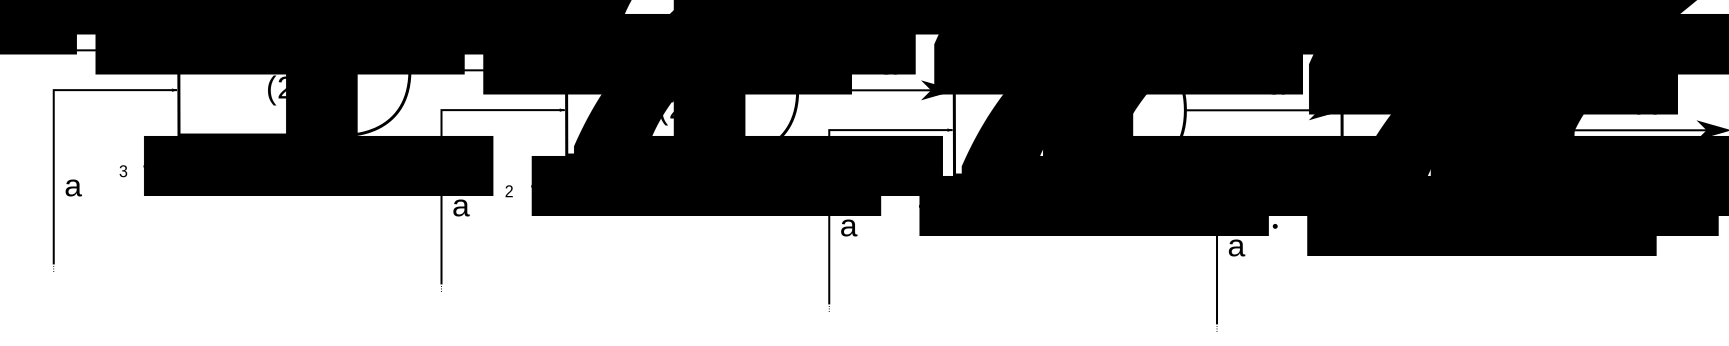
\includegraphics[width=1.0\linewidth]{Appendix_Infinite_Series/images/I-O_Process_Equivalence.pdf}
\caption{Process flows in a single-sector economy. ***** Mik: please update 
to include Biopshere (0), change ``Sector (2)'' to ``Production (1)'', 
and change all subscripts accordingly. ******}
\label{fig:single_sector_flows_3}
\end{figure}

The economy produces output at a rate of $\dot{X}_{1}$, 
but it requires energy from the biosphere 
($\dot{E}_{01} = a_{01}\dot{X}_{1}$) to do so. 
The economy also consumes a fraction 
of its own gross output 
($\dot{X}_{11} = a_{11}\dot{X}_{1}$). 
To produce $a_{11}\dot{X}_{1}$, 
the economy requires an additional $a_{01}a_{11}\dot{X}_{1}$ 
of energy from the biosphere. 
The sum of all direct energy ($\dot{E}$) required for the economy 
to produce at a rate of $\dot{X}_{1}$ is an infinite sum.

\begin{equation} \label{eq:E_dot_demand_SS}
	\dot{E}_{demand,tot} 
	= a_{01}\dot{X}_{1} 
	+ a_{01}a_{11}\dot{X}_{1} 
	+ a_{01}a_{11}^2\dot{X}_{1} 
	+ \ldots
\end{equation}

The energy intensity of the economy ($\varepsilon_{1}$) is 

\begin{equation} \label{eq:epsilon_process_SS_intermediate}
	\varepsilon_{1} 
	= \frac{\dot{E}_{demand,tot}}{\dot{X}_{1}} 
	= a_{01}(1 + a_{11} + a_{11}^2 + \ldots) 
	= a_{01}\sum_{n=0}^{\infty}a_{11}^{n}.
\end{equation}

Realizing that 
$\sum\limits_{n=0}^{\infty}a_{11}^{n} 
= \frac{1}{1-a_{11}}$ 
and 
$a_{01} 
= \frac{\dot{E}_{01}}{\dot{X}_{1}}$ 
(direct energy can be considered the output of the biosphere
in this situation) gives

\begin{equation} \label{eq:epsilon_process_SS}
	\varepsilon_{1} = {(1-a_{11})}^{-1} \dot{X}^{-1} \dot{E}_{01}.
\end{equation}

Neglecting 
accumulation of embodied energy in the economy
$\left( \frac{\mathrm{d}B_{1}}{\mathrm{d}t} = 0 \right)$
and depreciation $\left( \gamma_{1}B_{1} = 0 \right)$,
\index{depreciation}
Equations~\ref{eq:eps3_ss_IO} and~\ref{eq:epsilon_process_SS} are identical, 
indicating that the I-O approach accounts 
for the infinite recursion of energy demand by the economy.
****** Fix this paragraph after editing Chapter 6. *****


\bibliographystyle{unsrt}
\bibliography{../EROI_review_v2}


% Always give a unique label
% and use \ref{<label>} for cross-references
% and \cite{<label>} for bibliographic references
% use \sectionmark{}
% to alter or adjust the section heading in the running head
%% Instead of simply listing headings of different levels we recommend to let every heading be followed by at least a short passage of text. Furtheron please use the \LaTeX\ automatism for all your cross-references and citations.

%% Please note that the first line of text that follows a heading is not indented, whereas the first lines of all sequent paragraphs are.

%% Use the standard \verb|equation| environment to typeset your equations, e.g.
%
%% \begin{equation}
%% a \times b = c\;,
%% \end{equation}
%
%% however, for multiline equations we recommend to use the \verb|eqnarray|
%% environment\footnote{In physics texts please activate the class option \texttt{vecphys} to depict your vectors in \textbf{\itshape boldface-italic} type - as is customary for a wide range of physical jects.}.
%% \begin{eqnarray}
%% a \times b = c \nonumber\\
%% \vec{a} \cdot \vec{b}=\vec{c}
%% \label{eq:01}
%% \end{eqnarray}

%% \section{section Heading}
%% \label{sec:2}
%% Instead of simply listing headings of different levels we recommend to let every heading be followed by at least a short passage of text. Furtheron please use the \LaTeX\ automatism for all your cross-references\index{cross-references} and citations\index{citations} as has already been described in Sect.~\ref{sec:2}.

%% \begin{quotation}
%% Please do not use quotation marks when quoting texts! Simply use the \verb|quotation| environment -- it will automatically render Springer's preferred layout.
%% \end{quotation}


%% \section{section Heading}
%% Instead of simply listing headings of different levels we recommend to let every heading be followed by at least a short passage of text. Furtheron please use the \LaTeX\ automatism for all your cross-references and citations as has already been described in Sect.~\ref{sec:2}, see also Fig.~\ref{fig:1}\footnote{If you copy text passages, figures, or tables from other works, you must obtain \textit{permission} from the copyright holder (usually the original publisher). Please enclose the signed permission with the manucript. The sources\index{permission to print} must be acknowledged either in the captions, as footnotes or in a separate section of the book.}

%% Please note that the first line of text that follows a heading is not indented, whereas the first lines of all sequent paragraphs are.

% For figures use
%
%% \begin{figure}[b]
%% \sidecaption
% Use the relevant command for your figure-insertion program
% to insert the figure file.
% For example, with the option graphics use
%% \includegraphics[scale=.65]{figure}
%
% If not, use
%\picplace{5cm}{2cm} % Give the correct figure height and width in cm
%
%% \caption{If the width of the figure is less than 7.8 cm use the \texttt{sidecapion} command to flush the caption on the left side of the page. If the figure is positioned at the top of the page, align the sidecaption with the top of the figure -- to achieve this you simply need to use the optional argument \texttt{[t]} with the \texttt{sidecaption} command}
%% \label{fig:1}       % Give a unique label
%% \end{figure}


%% \paragraph{Paragraph Heading} %
%% Instead of simply listing headings of different levels we recommend to let every heading be followed by at least a short passage of text. Furtheron please use the \LaTeX\ automatism for all your cross-references and citations as has already been described in Sect.~\ref{sec:2}.

%% Please note that the first line of text that follows a heading is not indented, whereas the first lines of all sequent paragraphs are.

%% For typesetting numbered lists we recommend to use the \verb|enumerate| environment -- it will automatically render Springer's preferred layout.

%% \begin{enumerate}
%% \item{Livelihood and survival mobility are oftentimes coutcomes of uneven socioeconomic development.}
%% \begin{enumerate}
%% \item{Livelihood and survival mobility are oftentimes coutcomes of uneven socioeconomic development.}
%% \item{Livelihood and survival mobility are oftentimes coutcomes of uneven socioeconomic development.}
%% \end{enumerate}
%% \item{Livelihood and survival mobility are oftentimes coutcomes of uneven socioeconomic development.}
%% \end{enumerate}


%% \paragraph{paragraph Heading} In order to avoid simply listing headings of different levels we recommend to let every heading be followed by at least a short passage of text. Use the \LaTeX\ automatism for all your cross-references and citations as has already been described in Sect.~\ref{sec:2}, see also Fig.~\ref{fig:2}.

%% Please note that the first line of text that follows a heading is not indented, whereas the first lines of all sequent paragraphs are.

%% For unnumbered list we recommend to use the \verb|itemize| environment -- it will automatically render Springer's preferred layout.

%% \begin{itemize}
%% \item{Livelihood and survival mobility are oftentimes coutcomes of uneven socioeconomic development, cf. Table~\ref{tab:1}.}
%% \begin{itemize}
%% \item{Livelihood and survival mobility are oftentimes coutcomes of uneven socioeconomic development.}
%% \item{Livelihood and survival mobility are oftentimes coutcomes of uneven socioeconomic development.}
%% \end{itemize}
%% \item{Livelihood and survival mobility are oftentimes coutcomes of uneven socioeconomic development.}
%% \end{itemize}

%% \begin{figure}[t]
%% \sidecaption[t]
% Use the relevant command for your figure-insertion program
% to insert the figure file.
% For example, with the option graphics use
%% \includegraphics[scale=.65]{figure}
%
% If not, use
%\picplace{5cm}{2cm} % Give the correct figure height and width in cm
%
%% \caption{Please write your figure caption here}
%% \label{fig:2}       % Give a unique label
%% \end{figure}

%% \runinhead{Run-in Heading Boldface Version} Use the \LaTeX\ automatism for all your cross-references and citations as has already been described in Sect.~\ref{sec:2}.

%% \runinhead{Run-in Heading Italic Version} Use the \LaTeX\ automatism for all your cross-refer\-ences and citations as has already been described in Sect.~\ref{sec:2}\index{paragraph}.
% Use the \index{} command to code your index words
%
% For tables use
%
%% \begin{table}
%% \caption{Please write your table caption here}
%% \label{tab:1}       % Give a unique label
%
% For LaTeX tables use
%
%% \begin{tabular}{p{2cm}p{2.4cm}p{2cm}p{4.9cm}}
%% \hline\noalign{\smallskip}
%% Classes & class & Length & Action Mechanism  \\
%% \noalign{\smallskip}\svhline\noalign{\smallskip}
%% Translation & mRNA$^a$  & 22 (19--25) & Translation repression, mRNA cleavage\\
%% Translation & mRNA cleavage & 21 & mRNA cleavage\\
%% Translation & mRNA  & 21--22 & mRNA cleavage\\
%%Translation & mRNA  & 24--26 & Histone and DNA Modification\\
%%\noalign{\smallskip}\hline\noalign{\smallskip}
%%\end{tabular}
%%$^a$ Table foot note (with superscript)
%%\end{table}
%
%% \section{Section Heading}
%%\label{sec:3}
% Always give a unique label
% and use \ref{<label>} for cross-references
% and \cite{<label>} for bibliographic references
% use \sectionmark{}
% to alter or adjust the section heading in the running head
%% Instead of simply listing headings of different levels we recommend to let every heading be followed by at least a short passage of text. Furtheron please use the \LaTeX\ automatism for all your cross-references and citations as has already been described in Sect.~\ref{sec:2}.

%% Please note that the first line of text that follows a heading is not indented, whereas the first lines of all sequent paragraphs are.

%%If you want to list definitions or the like we recommend to use the Springer-enhanced \verb|description| environment -- it will automatically render Springer's preferred layout.

%%\begin{description}[Type 1]
%%\item[Type 1]{That addresses central themes pertainng to migration, health, and disease. In Sect.~\ref{sec:1}, Wilson discusses the role of human migration in infectious disease distributions and patterns.}
%%\item[Type 2]{That addresses central themes pertainng to migration, health, and disease. In Sect.~\ref{sec:2}, Wilson discusses the role of human migration in infectious disease distributions and patterns.}
%%\end{description}

%%\section{section Heading} %
%% In order to avoid simply listing headings of different levels we recommend to let every heading be followed by at least a short passage of text. Use the \LaTeX\ automatism for all your cross-references and citations citations as has already been described in Sect.~\ref{sec:2}.

%% Please note that the first line of text that follows a heading is not indented, whereas the first lines of all sequent paragraphs are.

%% \begin{svgraybox}
%% If you want to emphasize complete paragraphs of texts we recommend to use the newly defined Springer class option \verb|graybox| and the newly defined environment \verb|svgraybox|. This will produce a 15 percent screened box 'behind' your text.

%% If you want to emphasize complete paragraphs of texts we recommend to use the newly defined Springer class option and environment \verb|svgraybox|. This will produce a 15 percent screened box 'behind' your text.
%% \end{svgraybox}


%% \section{section Heading}
%%Instead of simply listing headings of different levels we recommend to let every heading be followed by at least a short passage of text. Furtheron please use the \LaTeX\ automatism for all your cross-references and citations as has already been described in Sect.~\ref{sec:2}.

%% Please note that the first line of text that follows a heading is not indented, whereas the first lines of all sequent paragraphs are.

%% \begin{theorem}
%% Theorem text goes here.
%% \end{theorem}
%
% or
%
%% \begin{definition}
%% Definition text goes here.
%% \end{definition}

%% \begin{proof}
%\smartqed
%% Proof text goes here.
%% \qed
%% \end{proof}

%%\paragraph{Paragraph Heading} %
%% Instead of simply listing headings of different levels we recommend to let every heading be followed by at least a short passage of text. Furtheron please use the \LaTeX\ automatism for all your cross-references and citations as has already been described in Sect.~\ref{sec:2}.

%% Note that the first line of text that follows a heading is not indented, whereas the first lines of all subsequent paragraphs are.
%
% For built-in environments use
%
%%\begin{theorem}
%%Theorem text goes here.
%%\end{theorem}
%
%%\begin{definition}
%%Definition text goes here.
%%\end{definition}
%
%%\begin{proof}
%%\smartqed
%% Proof text goes here.
%%\qed
%%\end{proof}
%
%% \begin{acknowledgement}
%% If you want to include acknowledgments of assistance and the like at the end of an individual chapter please use the \verb|acknowledgement| environment -- it will automatically render Springer's preferred layout.
%% \end{acknowledgement}
%
%% \section*{Appendix}
%% \addcontentsline{toc}{section}{Appendix}
%
%% When placed at the end of a chapter or contribution (as opposed to at the end of the book), the numbering of tables, figures, and equations in the appendix section continues on from that in the main text. Hence please \textit{do not} use the \verb|appendix| command when writing an appendix at the end of your chapter or contribution. If there is only one the appendix is designated ``Appendix'', or ``Appendix 1'', or ``Appendix 2'', etc. if there is more than one.

%% \begin{equation}
%% a \times b = c
%% \end{equation}
% Problems or Exercises should be sorted chapterwise
%% \section*{Problems}
%% \addcontentsline{toc}{section}{Problems}
%
% Use the following environment.
% Don't forget to label each problem;
% the label is needed for the solutions' environment
%% \begin{prob}
%% \label{prob1}
%% A given problem or Excercise is described here. The
%% problem is described here. The problem is described here.
%% \end{prob}

%% \begin{prob}
%% \label{prob2}
%% \textbf{Problem Heading}\\
%% (a) The first part of the problem is described here.\\
%% (b) The second part of the problem is described here.
%% \end{prob}




%!TEX root = ../Heun_Dale_Haney_A_dynamic_approach_to_input_output_modeling.tex
%%%%%%%%%%%%%%%%%%%%% appendix.tex %%%%%%%%%%%%%%%%%%%%%%%%%%%%%%%%%
%
% sample appendix
%
% Use this file as a template for your own input.
%
%%%%%%%%%%%%%%%%%%%%%%%% Springer-Verlag %%%%%%%%%%%%%%%%%%%%%%%%%%

%\motto{All's well that ends well}
%%%%%%%%%%%%%%%%%%%%%%%%%%%%%%%%
%%%%%%%%%% Appendix A %%%%%%%%%%
%%%%%%%%%%%%%%%%%%%%%%%%%%%%%%%%
\chapter{Proof of Equation~\ref{eq:Xdifference1} 
and method for estimating the input-output matrix ($\vec{A}$)}
% Always give a unique label
\label{app:Proof} 
% use \chaptermark{} to alter or adjust the chapter heading in the running head
\chaptermark{Appendix A}
%%%%%%%%%%%%%%%%%%%%%%%%%%%%%%%%
%%%%%%%%%%%%%%%%%%%%%%%%%%%%%%%%
%%%%%%%%%%%%%%%%%%%%%%%%%%%%%%%%

%Use the template \emph{appendix.tex} together with the Springer document class SVMono (monograph-type books) or SVMult (edited books) to style appendix of your book in the Springer layout.


We begin with a restatement of Equation~\ref{eq:Xdifference1}.

\begin{equation} \label{eq:Xdifference1Proof-1}
	\vec{X}_{t}^\mathrm{T} 
	- \hat{\vec{X}} 
	= \hat{\vec{X}}(\vec{A}^\mathrm{T} - \vec{I})
\end{equation}

\noindent We expand the matrices to obtain

\begin{equation} \label{eq:Xdifference1Proof-2}
	\begin{bmatrix}
		\dot{X}_{22} & \dot{X}_{32}	\\
		\dot{X}_{23} & \dot{X}_{33}
	\end{bmatrix}
	-
	\begin{bmatrix}
		\dot{X}_{2} & 0	\\
		0           & \dot{X}_{3}
	\end{bmatrix}
	=
	\begin{bmatrix}
		\dot{X}_{2} & 0	\\
		0           & \dot{X}_{3}
	\end{bmatrix}
	\begin{bmatrix}
		a_{22}-1 & a_{32}	\\
		a_{23}   & a_{33}-1
	\end{bmatrix}.
\end{equation}

\noindent Subtracting and multiplying matrices gives

\begin{equation} \label{eq:Xdifference1Proof-3}
	\begin{bmatrix} 	
		\dot{X}_{22} - \dot{X}_{2} & \dot{X}_{32}	\\
		\dot{X}_{23}               & \dot{X}_{33} - \dot{X}_{3}
	\end{bmatrix}
	=
	\begin{bmatrix} 	
		\dot{X}_{2} a_{22} - \dot{X}_{2} & \dot{X}_{2} a_{32}	\\
		\dot{X}_{3} a_{23}               & \dot{X}_{3} a_{33} - \dot{X}_{3}
	\end{bmatrix}.
\end{equation}

\noindent Using $\dot{X}_j a_{ij} = \dot{X}_{ij}$ (see Equation~\ref{eq:aij_def}) gives

\begin{equation} \label{eq:Xdifference1Proof-4}
	\begin{bmatrix} 	
		\dot{X}_{22} - \dot{X}_{2} & \dot{X}_{32}	\\
		\dot{X}_{23}               & \dot{X}_{33} - \dot{X}_{3}
	\end{bmatrix} 
	= 
	\begin{bmatrix} 	
		\dot{X}_{22} - \dot{X}_{2} & \dot{X}_{32}	\\
		\dot{X}_{23}               & \dot{X}_{33} - \dot{X}_{3}
	\end{bmatrix}
\end{equation}

\noindent to complete the proof.

Using Equation~\ref{eq:Xdifference1Proof-1}, 
we can derive an expression for estimating the input-output matrix ($\vec{A}$)
given sector outputs ($\hat{\vec{X}}$) and the transaction matrix ($\vec{X}_{t}$).
Premultiplying Equation~\ref{eq:Xdifference1Proof-1} by $\hat{\vec{X}}^{-1}$ gives

\begin{equation} \label{eq:Xdifference1Proof-5}
	\hat{\vec{X}}^{-1}
	\left( 
		\vec{X}_{t}^\mathrm{T} 
		- \hat{\vec{X}} 
	\right)
	= \vec{A}^\mathrm{T} - \vec{I}
\end{equation}

\noindent{}Further rearranging gives

\begin{equation}\label{eq:Xdifference1Proof-6}
	\vec{A}^\mathrm{T} 
	= \hat{\vec{X}}^{-1}
	\left( 
		\vec{X}_{t}^\mathrm{T} 
		- \hat{\vec{X}} 
	\right)
	+ \vec{I},
\end{equation}

\begin{equation}\label{eq:Xdifference1Proof-7}
	\vec{A}^\mathrm{T} 
	= \hat{\vec{X}}^{-1} \vec{X}_{t}^\mathrm{T} 
	- \hat{\vec{X}}^{-1} \hat{\vec{X}}
	+ \vec{I},	
\end{equation}

\begin{equation}\label{eq:Xdifference1Proof-8}
	\vec{A}^\mathrm{T} 
	= \hat{\vec{X}}^{-1} \vec{X}_{t}^\mathrm{T} 
	- \vec{I}
	+ \vec{I},	
\end{equation}

\begin{equation}\label{eq:Xdifference1Proof-9}
	\vec{A}^\mathrm{T} 
	= \hat{\vec{X}}^{-1} 
	\vec{X}_{t}^\mathrm{T},
\end{equation}

\noindent{}and

\begin{equation}\label{eq:Xdifference1Proof-10}
	\vec{A} 
	= \vec{X}_{t}
	\left( {\hat{\vec{X}}^{-1}} \right) ^\mathrm{T}.
\end{equation}

\noindent{}Realizing that $\hat{\vec{X}}$ and $\hat{\vec{X}}^{-1}$
are diagonal matrices gives

\begin{equation}\label{eq:Xdifference1Proof-11}
	\vec{A} 
	= \vec{X}_{t}
	\hat{\vec{X}}^{-1},
\end{equation}

\noindent{}which is an unsurprising result 
given the definition of the input-output ratio ($a$) in Equation~\ref{eq:aij_def}.

Equation~\ref{eq:Xdifference1Proof-11} provides a method 
of estimating the input-output matrix~($\vec{A}$) using
sector outputs~($\hat{\vec{X}}$) and the transaction matrix~($\vec{X}_{t}$).



%\section{Section Heading}
%\label{sec:A1}
%% Always give a unique label
%% and use \ref{<label>} for cross-references
%% and \cite{<label>} for bibliographic references
%% use \sectionmark{}
%% to alter or adjust the section heading in the running head
%Instead of simply listing headings of different levels we recommend to let every heading be followed by at least a short passage of text. Furtheron please use the \LaTeX\ automatism for all your cross-references and citations.
%
%
%\subsection{Subsection Heading}
%\label{sec:A2}
%Instead of simply listing headings of different levels we recommend to let every heading be followed by at least a short passage of text. Furtheron please use the \LaTeX\ automatism for all your cross-references and citations as has already been described in Sect.~\ref{sec:A1}.
%
%For multiline equations we recommend to use the \verb|eqnarray| environment.
%\begin{eqnarray}
%\vec{a}\times\vec{b}=\vec{c} \nonumber\\
%\vec{a}\times\vec{b}=\vec{c}
%\label{eq:A01}
%\end{eqnarray}
%
%\subsubsection{Subsubsection Heading}
%Instead of simply listing headings of different levels we recommend to let every heading be followed by at least a short passage of text. Furtheron please use the \LaTeX\ automatism for all your cross-references and citations as has already been described in Sect.~\ref{sec:A2}.
%
%Please note that the first line of text that follows a heading is not indented, whereas the first lines of all subsequent paragraphs are.
%
%% For figures use
%%
%\begin{figure}[t]
%\sidecaption[t]
%%\centering
%% Use the relevant command for your figure-insertion program
%% to insert the figure file.
%% For example, with the option graphics use
%\includegraphics[scale=.65]{figure}
%%
%% If not, use
%%\picplace{5cm}{2cm} % Give the correct figure height and width in cm
%%
%\caption{Please write your figure caption here}
%\label{fig:A1}       % Give a unique label
%\end{figure}
%
%% For tables use
%%
%\begin{table}
%\caption{Please write your table caption here}
%\label{tab:A1}       % Give a unique label
%%
%% For LaTeX tables use
%%
%\begin{tabular}{p{2cm}p{2.4cm}p{2cm}p{4.9cm}}
%\hline\noalign{\smallskip}
%Classes & Subclass & Length & Action Mechanism  \\
%\noalign{\smallskip}\hline\noalign{\smallskip}
%Translation & mRNA$^a$  & 22 (19--25) & Translation repression, mRNA cleavage\\
%Translation & mRNA cleavage & 21 & mRNA cleavage\\
%Translation & mRNA  & 21--22 & mRNA cleavage\\
%Translation & mRNA  & 24--26 & Histone and DNA Modification\\
%\noalign{\smallskip}\hline\noalign{\smallskip}
%\end{tabular}
%$^a$ Table foot note (with superscript)
%\end{table}
%%


%!TEX root = ../Heun_Dale_Haney_A_dynamic_approach_to_input_output_modeling.tex
%%%%%%%%%%%%%%%%%%%%% appendix.tex %%%%%%%%%%%%%%%%%%%%%%%%%%%%%%%%%
%
% sample appendix
%
% Use this file as a template for your own input.
%
%%%%%%%%%%%%%%%%%%%%%%%% Springer-Verlag %%%%%%%%%%%%%%%%%%%%%%%%%%

%\motto{All's well that ends well}
%%%%%%%%%%%%%%%%%%%%%%%%%%%%%%%%
%%%%%%%%%% Appendix A %%%%%%%%%%
%%%%%%%%%%%%%%%%%%%%%%%%%%%%%%%%
\chapter{Estimating the input-output matrix ($\vec{A}$)}
% Always give a unique label
\label{chap:Estimating_A} 
% use \chaptermark{} to alter or adjust the chapter heading in the running head
\chaptermark{estimating $\vec{A}$}
%%%%%%%%%%%%%%%%%%%%%%%%%%%%%%%%
%%%%%%%%%%%%%%%%%%%%%%%%%%%%%%%%
%%%%%%%%%%%%%%%%%%%%%%%%%%%%%%%%

%Use the template \emph{appendix.tex} together with the Springer document class SVMono (monograph-type books) or SVMult (edited books) to style appendix of your book in the Springer layout.

Using Equation~\ref{eq:Xdifference1} (which is proved in Appendix~\ref{app:Proof}), 
we can derive an expression for estimating the input-output matrix ($\vec{A}$)
given sector outputs ($\hat{\vec{X}}$) and the transaction matrix ($\vec{X}_{t}$).
Premultiplying Equation~\ref{eq:Xdifference1} by $\hat{\vec{X}}^{-1}$ gives

\begin{equation} \label{eq:Xdifference1Proof-5}
	\hat{\vec{X}}^{-1}
	\left( 
		\vec{X}_{t}^\mathrm{T} 
		- \hat{\vec{X}} 
	\right)
	= \vec{A}^\mathrm{T} - \vec{I}
\end{equation}

\noindent{}Further rearranging gives

\begin{equation}\label{eq:Xdifference1Proof-6}
	\vec{A}^\mathrm{T} 
	= \hat{\vec{X}}^{-1}
	\left( 
		\vec{X}_{t}^\mathrm{T} 
		- \hat{\vec{X}} 
	\right)
	+ \vec{I},
\end{equation}

\begin{equation}\label{eq:Xdifference1Proof-7}
	\vec{A}^\mathrm{T} 
	= \hat{\vec{X}}^{-1} \vec{X}_{t}^\mathrm{T} 
	- \hat{\vec{X}}^{-1} \hat{\vec{X}}
	+ \vec{I},	
\end{equation}

\begin{equation}\label{eq:Xdifference1Proof-8}
	\vec{A}^\mathrm{T} 
	= \hat{\vec{X}}^{-1} \vec{X}_{t}^\mathrm{T} 
	- \vec{I}
	+ \vec{I},	
\end{equation}

\begin{equation}\label{eq:Xdifference1Proof-9}
	\vec{A}^\mathrm{T} 
	= \hat{\vec{X}}^{-1} 
	\vec{X}_{t}^\mathrm{T},
\end{equation}

\noindent{}and

\begin{equation}\label{eq:Xdifference1Proof-10}
	\vec{A} 
	= \vec{X}_{t}
	{\left( {\hat{\vec{X}}^{-1}} \right)}^\mathrm{T}.
\end{equation}

\noindent{}Realizing that $\hat{\vec{X}}$ and $\hat{\vec{X}}^{-1}$
are diagonal matrices gives

\begin{equation}\label{eq:Estimating_A_matrix} 
	\vec{A} 
	= \vec{X}_{t}
	\hat{\vec{X}}^{-1},
\end{equation}

\noindent{}Expanding the matrices of Equation~\ref{eq:Estimating_A_matrix} gives

\begin{equation}
	\vec{A}
	=
	\begin{bmatrix}
		\dot{X}_{11} & \dot{X}_{12} & \cdots \\
		\dot{X}_{21} & \dot{X}_{22} & \cdots \\
		\vdots       & \vdots       & \ddots
	\end{bmatrix}
	\begin{bmatrix}
		1/\dot{X}_{1} & 0             & \cdots \\
		0             & 1/\dot{X}_{2} & \cdots \\
		\vdots        & \vdots        & \ddots
	\end{bmatrix}
\end{equation}

\noindent{}and

\begin{equation}
	\vec{A}
	\equiv
	\begin{bmatrix}
		a_{11} & a_{12} & \cdots \\
		a_{21} & a_{22} & \cdots \\
		\vdots & \vdots & \ddots
	\end{bmatrix}
	=
	\begin{bmatrix}
		\frac{\dot{X}_{11}}{\dot{X}_{1}} & \frac{\dot{X}_{12}}{\dot{X}_{2}} & \cdots \\
		\frac{\dot{X}_{21}}{\dot{X}_{1}} & \frac{\dot{X}_{22}}{\dot{X}_{2}} & \cdots \\
		\vdots       & \vdots       & \ddots
	\end{bmatrix},
\end{equation}

\noindent{}as expected
given the definition of the input-output ratio ($a$) 
in Equation~\ref{eq:aij_def}

\begin{equation*}
	a_{ij} 
	\equiv \frac{\dot{X}_{ij}}{\dot{X}_{j}}.
\end{equation*}

Equation~\ref{eq:Estimating_A_matrix} provides a method 
of estimating the input-output matrix~($\vec{A}$) using
the transaction matrix~($\vec{X}_{t}$)
and sector outputs~($\hat{\vec{X}}$).



%\section{Section Heading}
%\label{sec:A1}
%% Always give a unique label
%% and use \ref{<label>} for cross-references
%% and \cite{<label>} for bibliographic references
%% use \sectionmark{}
%% to alter or adjust the section heading in the running head
%Instead of simply listing headings of different levels we recommend to let every heading be followed by at least a short passage of text. Furtheron please use the \LaTeX\ automatism for all your cross-references and citations.
%
%
%\subsection{Subsection Heading}
%\label{sec:A2}
%Instead of simply listing headings of different levels we recommend to let every heading be followed by at least a short passage of text. Furtheron please use the \LaTeX\ automatism for all your cross-references and citations as has already been described in Sect.~\ref{sec:A1}.
%
%For multiline equations we recommend to use the \verb|eqnarray| environment.
%\begin{eqnarray}
%\vec{a}\times\vec{b}=\vec{c} \nonumber\\
%\vec{a}\times\vec{b}=\vec{c}
%\label{eq:A01}
%\end{eqnarray}
%
%\subsubsection{Subsubsection Heading}
%Instead of simply listing headings of different levels we recommend to let every heading be followed by at least a short passage of text. Furtheron please use the \LaTeX\ automatism for all your cross-references and citations as has already been described in Sect.~\ref{sec:A2}.
%
%Please note that the first line of text that follows a heading is not indented, whereas the first lines of all subsequent paragraphs are.
%
%% For figures use
%%
%\begin{figure}[t]
%\sidecaption[t]
%%\centering
%% Use the relevant command for your figure-insertion program
%% to insert the figure file.
%% For example, with the option graphics use
%\includegraphics[scale=.65]{figure}
%%
%% If not, use
%%\picplace{5cm}{2cm} % Give the correct figure height and width in cm
%%
%\caption{Please write your figure caption here}
%\label{fig:A1}       % Give a unique label
%\end{figure}
%
%% For tables use
%%
%\begin{table}
%\caption{Please write your table caption here}
%\label{tab:A1}       % Give a unique label
%%
%% For LaTeX tables use
%%
%\begin{tabular}{p{2cm}p{2.4cm}p{2cm}p{4.9cm}}
%\hline\noalign{\smallskip}
%Classes & Subclass & Length & Action Mechanism  \\
%\noalign{\smallskip}\hline\noalign{\smallskip}
%Translation & mRNA$^a$  & 22 (19--25) & Translation repression, mRNA cleavage\\
%Translation & mRNA cleavage & 21 & mRNA cleavage\\
%Translation & mRNA  & 21--22 & mRNA cleavage\\
%Translation & mRNA  & 24--26 & Histone and DNA Modification\\
%\noalign{\smallskip}\hline\noalign{\smallskip}
%\end{tabular}
%$^a$ Table foot note (with superscript)
%\end{table}
%%


%!TEX root = ../Heun_Dale_Haney_A_dynamic_approach_to_input_output_modeling.tex
%%%%%%%%%%%%%%%%%%%%% chapter.tex %%%%%%%%%%%%%%%%%%%%%%%%%%%%%%%%%
%
% sample chapter
%
% Use this file as a template for your own input.
%
%%%%%%%%%%%%%%%%%%%%%%%% Springer-Verlag %%%%%%%%%%%%%%%%%%%%%%%%%%
%\motto{Use the template \emph{chapter.tex} to style the various elements of your chapter content.}
\chapter{Column vs.\ row vectors in energy intensity equations}
% Always give a unique label
\label{chap:Casler} 
% use \chaptermark{} to alter or adjust the chapter heading in the running head
\chaptermark{column and row vectors}


In this manuscript, we choose to define 
energy intensity ($\bm{\varepsilon}$) and 
energy input ($\vec{E}_{0}$~and~$\vec{T}_{1}$)
as a column vectors (see Equations~\ref{eq:eps_vec_def},~\ref{eq:E_vec_def}, 
and~\ref{eq:T_vec_def}, respectively),
because it natural to solve a system of equations
for a column vector rather than a row vector.
And, Equation~\ref{eq:C-Expanded_Matrix_Form} could not
be written as neatly if $\bm{\varepsilon}$ and $\vec{E}_{0}$
were row vectors.

In contrast, the I-O literature (see, 
e.g.,~\cite{Casler1984}~and~\cite{Bullard:1978vd})
defines energy intensity and energy input
as row vectors. 
The row vs.\ column difference is manifest in the appearance 
of the energy intensity matrix equation.

To demonstrate that our column vector formulation is equivalent 
to the literature's row vector formulation,
this appendix derives a column vector version of the energy intensity equation
that is often found in the literature.
The point of comparison is Casler~\cite{Casler1984}.
Casler's~\cite{Casler1984} energy intensity (Equation 6)
was derived from row vectors 
as\footnote{Equation~\ref{eq:Casler6-converted} is written according
to the variable conventions in this manuscript.
The literal Equation~6 in Casler~\cite{Casler1984} is
$
\varepsilon
= E \hat{X}^{-1} {(I - A)}^{-1}.
$
}

\begin{equation} \label{eq:Casler6-converted}
	\bm{\varepsilon}
	= \vec{E} 
		\hat{\vec{X}}^{-1}
		{(\vec{I} - \vec{A})}^{-1}.
\end{equation}

We begin with Equations~3 and~4 from Casler~\cite{Casler1984},
converted to overdot notation for rates.

\begin{equation} \label{eq:Casler-3}
	\varepsilon_{1} \dot{X}_{11}
	+ \varepsilon_{2} \dot{X}_{21}
	= \varepsilon_{1} \dot{X}_{1}
\end{equation}

\begin{equation} \label{eq:Casler-4}
	\varepsilon_{1} \dot{X}_{12}
	+ \varepsilon_{2} \dot{X}_{22}
	+ \dot{E}_{02}
	= \varepsilon_{2} \dot{X}_{2}
\end{equation}

\noindent{}Adding an $\dot{E}_{01}$ term\footnote{Note that 
$\dot{E}_{01} = 0$ for Casler~\cite{Casler1984}, 
so $\dot{E}_{0}$ can be included without changing Equation~\ref{eq:Casler-3}.} 
and utilizing matrix notation with column vectors 
(instead of row vectors) gives

\begin{equation} \label{eq:Casler34-matrix}
	\begin{bmatrix}
		\dot{X}_{11} & \dot{X}_{21} \\
		\dot{X}_{12} & \dot{X}_{22}
	\end{bmatrix}
	\begin{Bmatrix}
		\varepsilon_{1} \\
		\varepsilon_{2}
	\end{Bmatrix}
	+
	\begin{Bmatrix}
		\dot{E}_{01} \\
		\dot{E}_{02}
	\end{Bmatrix}
	=
	\begin{bmatrix}
		\dot{X}_{1} & 0 \\
		0           & \dot{X}_{2}
	\end{bmatrix}
	\begin{Bmatrix}
		\varepsilon_{1} \\
		\varepsilon_{2}
	\end{Bmatrix}.
\end{equation}

\noindent{}Substituting $\dot{X}_{ij} = a_{ij} \dot{X}_{j}$ (from 
Equation~\ref{eq:aij_def}) gives

\begin{equation} \label{eq:Casler34-matrix-with-a}
	\begin{bmatrix}
		a_{11} \dot{X}_{1} & a_{21} \dot{X}_{1} \\
		a_{12} \dot{X}_{2} & a_{22} \dot{X}_{2}
	\end{bmatrix}
	\begin{Bmatrix}
		\varepsilon_{1} \\
		\varepsilon_{2}
	\end{Bmatrix}
	+
	\begin{Bmatrix}
		\dot{E}_{01} \\
		\dot{E}_{02}
	\end{Bmatrix}
	=
	\begin{bmatrix}
		\dot{X}_{1} & 0 \\
		0           & \dot{X}_{2}
	\end{bmatrix}
	\begin{Bmatrix}
		\varepsilon_{1} \\
		\varepsilon_{2}
	\end{Bmatrix}.
\end{equation}

\noindent{}Expanding Equation~\ref{eq:Casler34-matrix-with-a} gives

\begin{equation} \label{eq:Casler34-matrix-expanded}
	\begin{bmatrix}
		\dot{X}_{1} & 0 \\
		0           & \dot{X}_{2}
	\end{bmatrix}
	\begin{bmatrix}
		a_{11} & a_{21} \\
		a_{12} & a_{22}
	\end{bmatrix}
	\begin{Bmatrix}
		\varepsilon_{1} \\
		\varepsilon_{2}
	\end{Bmatrix}
	+
	\begin{Bmatrix}
		\dot{E}_{01} \\
		\dot{E}_{02}
	\end{Bmatrix}
	=
	\begin{bmatrix}
		\dot{X}_{1} & 0 \\
		0           & \dot{X}_{2}
	\end{bmatrix}
	\begin{Bmatrix}
		\varepsilon_{1} \\
		\varepsilon_{2}
	\end{Bmatrix}.
\end{equation}

\noindent{}With the definitions of $\hat{\vec{X}}$,
$\vec{A}$, $\bm{\varepsilon}$, and $\vec{E}_{0}$
from Equations~\ref{eq:X_hat_matrix_def},
\ref{eq:A_matrix_def},~\ref{eq:E_vec_def}, 
and~\ref{eq:eps_vec_def}, respectively,
we can rewrite Equation~\ref{eq:Casler34-matrix-expanded} as

\begin{equation}
	\hat{\vec{X}} \vec{A}^{\mathrm{T}} \bm{\varepsilon}
	+ \vec{E}_{0}
	= \hat{\vec{X}} \bm{\varepsilon}.
\end{equation}

\noindent{}Solving for $\bm{\varepsilon}$ gives

\begin{equation} \label{eq:Casler6-column-vector}
	\bm{\varepsilon}
	= {(\vec{I} - \vec{A}^{\mathrm{T}})}^{-1} 
		\hat{\vec{X}}^{-1} 
		\vec{E}_{0}.
\end{equation}

The differences between Equations~\ref{eq:Casler6-converted}
and~\ref{eq:Casler6-column-vector} are due to the choice 
of row vectors (for Equation~\ref{eq:Casler6-converted})
or column vectors (for Equation~\ref{eq:Casler6-column-vector}) only.
Note that Equation~\ref{eq:Casler6-column-vector} is similar
to Equation~\ref{eq:epsilon_leontief_with_A}.
A detailed discussion of the differences 
between Equations~\ref{eq:Casler6-column-vector} and~\ref{eq:epsilon_leontief_with_A}
can be found in Section~\ref{sec:Implications_for_IO}.


\bibliographystyle{unsrt}
\bibliography{../EROI_review_v2}


% Always give a unique label
% and use \ref{<label>} for cross-references
% and \cite{<label>} for bibliographic references
% use \sectionmark{}
% to alter or adjust the section heading in the running head
%% Instead of simply listing headings of different levels we recommend to let every heading be followed by at least a short passage of text. Furtheron please use the \LaTeX\ automatism for all your cross-references and citations.

%% Please note that the first line of text that follows a heading is not indented, whereas the first lines of all sequent paragraphs are.

%% Use the standard \verb|equation| environment to typeset your equations, e.g.
%
%% \begin{equation}
%% a \times b = c\;,
%% \end{equation}
%
%% however, for multiline equations we recommend to use the \verb|eqnarray|
%% environment\footnote{In physics texts please activate the class option \texttt{vecphys} to depict your vectors in \textbf{\itshape boldface-italic} type - as is customary for a wide range of physical jects.}.
%% \begin{eqnarray}
%% a \times b = c \nonumber\\
%% \vec{a} \cdot \vec{b}=\vec{c}
%% \label{eq:01}
%% \end{eqnarray}

%% \section{section Heading}
%% \label{sec:2}
%% Instead of simply listing headings of different levels we recommend to let every heading be followed by at least a short passage of text. Furtheron please use the \LaTeX\ automatism for all your cross-references\index{cross-references} and citations\index{citations} as has already been described in Sect.~\ref{sec:2}.

%% \begin{quotation}
%% Please do not use quotation marks when quoting texts! Simply use the \verb|quotation| environment -- it will automatically render Springer's preferred layout.
%% \end{quotation}


%% \section{section Heading}
%% Instead of simply listing headings of different levels we recommend to let every heading be followed by at least a short passage of text. Furtheron please use the \LaTeX\ automatism for all your cross-references and citations as has already been described in Sect.~\ref{sec:2}, see also Fig.~\ref{fig:1}\footnote{If you copy text passages, figures, or tables from other works, you must obtain \textit{permission} from the copyright holder (usually the original publisher). Please enclose the signed permission with the manucript. The sources\index{permission to print} must be acknowledged either in the captions, as footnotes or in a separate section of the book.}

%% Please note that the first line of text that follows a heading is not indented, whereas the first lines of all sequent paragraphs are.

% For figures use
%
%% \begin{figure}[b]
%% \sidecaption
% Use the relevant command for your figure-insertion program
% to insert the figure file.
% For example, with the option graphics use
%% \includegraphics[scale=.65]{figure}
%
% If not, use
%\picplace{5cm}{2cm} % Give the correct figure height and width in cm
%
%% \caption{If the width of the figure is less than 7.8 cm use the \texttt{sidecapion} command to flush the caption on the left side of the page. If the figure is positioned at the top of the page, align the sidecaption with the top of the figure -- to achieve this you simply need to use the optional argument \texttt{[t]} with the \texttt{sidecaption} command}
%% \label{fig:1}       % Give a unique label
%% \end{figure}


%% \paragraph{Paragraph Heading} %
%% Instead of simply listing headings of different levels we recommend to let every heading be followed by at least a short passage of text. Furtheron please use the \LaTeX\ automatism for all your cross-references and citations as has already been described in Sect.~\ref{sec:2}.

%% Please note that the first line of text that follows a heading is not indented, whereas the first lines of all sequent paragraphs are.

%% For typesetting numbered lists we recommend to use the \verb|enumerate| environment -- it will automatically render Springer's preferred layout.

%% \begin{enumerate}
%% \item{Livelihood and survival mobility are oftentimes coutcomes of uneven socioeconomic development.}
%% \begin{enumerate}
%% \item{Livelihood and survival mobility are oftentimes coutcomes of uneven socioeconomic development.}
%% \item{Livelihood and survival mobility are oftentimes coutcomes of uneven socioeconomic development.}
%% \end{enumerate}
%% \item{Livelihood and survival mobility are oftentimes coutcomes of uneven socioeconomic development.}
%% \end{enumerate}


%% \paragraph{paragraph Heading} In order to avoid simply listing headings of different levels we recommend to let every heading be followed by at least a short passage of text. Use the \LaTeX\ automatism for all your cross-references and citations as has already been described in Sect.~\ref{sec:2}, see also Fig.~\ref{fig:2}.

%% Please note that the first line of text that follows a heading is not indented, whereas the first lines of all sequent paragraphs are.

%% For unnumbered list we recommend to use the \verb|itemize| environment -- it will automatically render Springer's preferred layout.

%% \begin{itemize}
%% \item{Livelihood and survival mobility are oftentimes coutcomes of uneven socioeconomic development, cf. Table~\ref{tab:1}.}
%% \begin{itemize}
%% \item{Livelihood and survival mobility are oftentimes coutcomes of uneven socioeconomic development.}
%% \item{Livelihood and survival mobility are oftentimes coutcomes of uneven socioeconomic development.}
%% \end{itemize}
%% \item{Livelihood and survival mobility are oftentimes coutcomes of uneven socioeconomic development.}
%% \end{itemize}

%% \begin{figure}[t]
%% \sidecaption[t]
% Use the relevant command for your figure-insertion program
% to insert the figure file.
% For example, with the option graphics use
%% \includegraphics[scale=.65]{figure}
%
% If not, use
%\picplace{5cm}{2cm} % Give the correct figure height and width in cm
%
%% \caption{Please write your figure caption here}
%% \label{fig:2}       % Give a unique label
%% \end{figure}

%% \runinhead{Run-in Heading Boldface Version} Use the \LaTeX\ automatism for all your cross-references and citations as has already been described in Sect.~\ref{sec:2}.

%% \runinhead{Run-in Heading Italic Version} Use the \LaTeX\ automatism for all your cross-refer\-ences and citations as has already been described in Sect.~\ref{sec:2}\index{paragraph}.
% Use the \index{} command to code your index words
%
% For tables use
%
%% \begin{table}
%% \caption{Please write your table caption here}
%% \label{tab:1}       % Give a unique label
%
% For LaTeX tables use
%
%% \begin{tabular}{p{2cm}p{2.4cm}p{2cm}p{4.9cm}}
%% \hline\noalign{\smallskip}
%% Classes & class & Length & Action Mechanism  \\
%% \noalign{\smallskip}\svhline\noalign{\smallskip}
%% Translation & mRNA$^a$  & 22 (19--25) & Translation repression, mRNA cleavage\\
%% Translation & mRNA cleavage & 21 & mRNA cleavage\\
%% Translation & mRNA  & 21--22 & mRNA cleavage\\
%%Translation & mRNA  & 24--26 & Histone and DNA Modification\\
%%\noalign{\smallskip}\hline\noalign{\smallskip}
%%\end{tabular}
%%$^a$ Table foot note (with superscript)
%%\end{table}
%
%% \section{Section Heading}
%%\label{sec:3}
% Always give a unique label
% and use \ref{<label>} for cross-references
% and \cite{<label>} for bibliographic references
% use \sectionmark{}
% to alter or adjust the section heading in the running head
%% Instead of simply listing headings of different levels we recommend to let every heading be followed by at least a short passage of text. Furtheron please use the \LaTeX\ automatism for all your cross-references and citations as has already been described in Sect.~\ref{sec:2}.

%% Please note that the first line of text that follows a heading is not indented, whereas the first lines of all sequent paragraphs are.

%%If you want to list definitions or the like we recommend to use the Springer-enhanced \verb|description| environment -- it will automatically render Springer's preferred layout.

%%\begin{description}[Type 1]
%%\item[Type 1]{That addresses central themes pertainng to migration, health, and disease. In Sect.~\ref{sec:1}, Wilson discusses the role of human migration in infectious disease distributions and patterns.}
%%\item[Type 2]{That addresses central themes pertainng to migration, health, and disease. In Sect.~\ref{sec:2}, Wilson discusses the role of human migration in infectious disease distributions and patterns.}
%%\end{description}

%%\section{section Heading} %
%% In order to avoid simply listing headings of different levels we recommend to let every heading be followed by at least a short passage of text. Use the \LaTeX\ automatism for all your cross-references and citations citations as has already been described in Sect.~\ref{sec:2}.

%% Please note that the first line of text that follows a heading is not indented, whereas the first lines of all sequent paragraphs are.

%% \begin{svgraybox}
%% If you want to emphasize complete paragraphs of texts we recommend to use the newly defined Springer class option \verb|graybox| and the newly defined environment \verb|svgraybox|. This will produce a 15 percent screened box 'behind' your text.

%% If you want to emphasize complete paragraphs of texts we recommend to use the newly defined Springer class option and environment \verb|svgraybox|. This will produce a 15 percent screened box 'behind' your text.
%% \end{svgraybox}


%% \section{section Heading}
%%Instead of simply listing headings of different levels we recommend to let every heading be followed by at least a short passage of text. Furtheron please use the \LaTeX\ automatism for all your cross-references and citations as has already been described in Sect.~\ref{sec:2}.

%% Please note that the first line of text that follows a heading is not indented, whereas the first lines of all sequent paragraphs are.

%% \begin{theorem}
%% Theorem text goes here.
%% \end{theorem}
%
% or
%
%% \begin{definition}
%% Definition text goes here.
%% \end{definition}

%% \begin{proof}
%\smartqed
%% Proof text goes here.
%% \qed
%% \end{proof}

%%\paragraph{Paragraph Heading} %
%% Instead of simply listing headings of different levels we recommend to let every heading be followed by at least a short passage of text. Furtheron please use the \LaTeX\ automatism for all your cross-references and citations as has already been described in Sect.~\ref{sec:2}.

%% Note that the first line of text that follows a heading is not indented, whereas the first lines of all subsequent paragraphs are.
%
% For built-in environments use
%
%%\begin{theorem}
%%Theorem text goes here.
%%\end{theorem}
%
%%\begin{definition}
%%Definition text goes here.
%%\end{definition}
%
%%\begin{proof}
%%\smartqed
%% Proof text goes here.
%%\qed
%%\end{proof}
%
%% \begin{acknowledgement}
%% If you want to include acknowledgments of assistance and the like at the end of an individual chapter please use the \verb|acknowledgement| environment -- it will automatically render Springer's preferred layout.
%% \end{acknowledgement}
%
%% \section*{Appendix}
%% \addcontentsline{toc}{section}{Appendix}
%
%% When placed at the end of a chapter or contribution (as opposed to at the end of the book), the numbering of tables, figures, and equations in the appendix section continues on from that in the main text. Hence please \textit{do not} use the \verb|appendix| command when writing an appendix at the end of your chapter or contribution. If there is only one the appendix is designated ``Appendix'', or ``Appendix 1'', or ``Appendix 2'', etc. if there is more than one.

%% \begin{equation}
%% a \times b = c
%% \end{equation}
% Problems or Exercises should be sorted chapterwise
%% \section*{Problems}
%% \addcontentsline{toc}{section}{Problems}
%
% Use the following environment.
% Don't forget to label each problem;
% the label is needed for the solutions' environment
%% \begin{prob}
%% \label{prob1}
%% A given problem or Excercise is described here. The
%% problem is described here. The problem is described here.
%% \end{prob}

%% \begin{prob}
%% \label{prob2}
%% \textbf{Problem Heading}\\
%% (a) The first part of the problem is described here.\\
%% (b) The second part of the problem is described here.
%% \end{prob}





\backmatter%%%%%%%%%%%%%%%%%%%%%%%%%%%%%%%%%%%%%%%%%%%%%%%%%%%%%%%
%%!TEX root = ../Heun_Dale_Haney_A_dynamic_approach_to_input_output_modeling.tex

%%%%%%%%%%%%%%%%%%%%%%%%%%%%%%%%%%%%%%%%%%%%%%%%%%%%%%%%%%%%%%%%%%%
%%%%%%%%%%%%%%%%%%%%%%%%%%%%%%%%%%%%%%%%%%%%%%%%%%%%%%%%%%%%%%%%%%%
% This file contins information for the acronym section.
% Acronyms is built with the glossaries package.
%%%%%%%%%%%%%%%%%%%%%%%%%%%%%%%%%%%%%%%%%%%%%%%%%%%%%%%%%%%%%%%%%%%
%%%%%%%%%%%%%%%%%%%%%%%%%%%%%%%%%%%%%%%%%%%%%%%%%%%%%%%%%%%%%%%%%%%

% Define the glossary database for the nomenclature section
\newglossary{glossary}{gloin}{gloout}{Glossary}

%%%%%%%%%%%%%%%%%%%%%%%%%%%%%%%%%%%%%
% Provide Glossary entries.
%
% Fields of the glossary entries are:
%    key: the unnamed argument right after \newglossaryentry{_key_}{params}.
%         Convention: Let's adopt the convention that ALL keys are ALL lower-case 
%                     and prefixed by "glo:". This prevents conflicts with the Index.
%    name: how the symbol will appear in the Glossary
%    description: the description of the term.
%    sort: how the entry will be sorted in the Index. If omitted, name is used.
%%%%%%%%%%%%%%%%%%%%%%%%%%%%%%%%%%%%%
\newglossaryentry{glo:nea}{type = glossary, 
								name = NEA,
								description = Net Energy Analysis
								}


%\include{solutions}
\printindex{}

%%%%%%%%%%%%%%%%%%%%%%%%%%%%%%%%%%%%%%%%%%%%%%%%%%%%%%%%%%%%%%%%%%%%%%

\end{document}